\documentclass[twoside]{book}

% Packages required by doxygen
\usepackage{fixltx2e}
\usepackage{calc}
\usepackage{doxygen}
\usepackage[export]{adjustbox} % also loads graphicx
\usepackage{graphicx}
\usepackage[utf8]{inputenc}
\usepackage{makeidx}
\usepackage{multicol}
\usepackage{multirow}
\PassOptionsToPackage{warn}{textcomp}
\usepackage{textcomp}
\usepackage[nointegrals]{wasysym}
\usepackage[table]{xcolor}

% Font selection
\usepackage[T1]{fontenc}
\usepackage[scaled=.90]{helvet}
\usepackage{courier}
\usepackage{amssymb}
\usepackage{sectsty}
\renewcommand{\familydefault}{\sfdefault}
\allsectionsfont{%
  \fontseries{bc}\selectfont%
  \color{darkgray}%
}
\renewcommand{\DoxyLabelFont}{%
  \fontseries{bc}\selectfont%
  \color{darkgray}%
}
\newcommand{\+}{\discretionary{\mbox{\scriptsize$\hookleftarrow$}}{}{}}

% Page & text layout
\usepackage{geometry}
\geometry{%
  a4paper,%
  top=2.5cm,%
  bottom=2.5cm,%
  left=2.5cm,%
  right=2.5cm%
}
\tolerance=750
\hfuzz=15pt
\hbadness=750
\setlength{\emergencystretch}{15pt}
\setlength{\parindent}{0cm}
\setlength{\parskip}{3ex plus 2ex minus 2ex}
\makeatletter
\renewcommand{\paragraph}{%
  \@startsection{paragraph}{4}{0ex}{-1.0ex}{1.0ex}{%
    \normalfont\normalsize\bfseries\SS@parafont%
  }%
}
\renewcommand{\subparagraph}{%
  \@startsection{subparagraph}{5}{0ex}{-1.0ex}{1.0ex}{%
    \normalfont\normalsize\bfseries\SS@subparafont%
  }%
}
\makeatother

% Headers & footers
\usepackage{fancyhdr}
\pagestyle{fancyplain}
\fancyhead[LE]{\fancyplain{}{\bfseries\thepage}}
\fancyhead[CE]{\fancyplain{}{}}
\fancyhead[RE]{\fancyplain{}{\bfseries\leftmark}}
\fancyhead[LO]{\fancyplain{}{\bfseries\rightmark}}
\fancyhead[CO]{\fancyplain{}{}}
\fancyhead[RO]{\fancyplain{}{\bfseries\thepage}}
\fancyfoot[LE]{\fancyplain{}{}}
\fancyfoot[CE]{\fancyplain{}{}}
\fancyfoot[RE]{\fancyplain{}{\bfseries\scriptsize Generated by Doxygen }}
\fancyfoot[LO]{\fancyplain{}{\bfseries\scriptsize Generated by Doxygen }}
\fancyfoot[CO]{\fancyplain{}{}}
\fancyfoot[RO]{\fancyplain{}{}}
\renewcommand{\footrulewidth}{0.4pt}
\renewcommand{\chaptermark}[1]{%
  \markboth{#1}{}%
}
\renewcommand{\sectionmark}[1]{%
  \markright{\thesection\ #1}%
}

% Indices & bibliography
\usepackage{natbib}
\usepackage[titles]{tocloft}
\setcounter{tocdepth}{3}
\setcounter{secnumdepth}{5}
\makeindex

% Hyperlinks (required, but should be loaded last)
\usepackage{ifpdf}
\ifpdf
  \usepackage[pdftex,pagebackref=true]{hyperref}
\else
  \usepackage[ps2pdf,pagebackref=true]{hyperref}
\fi
\hypersetup{%
  colorlinks=true,%
  linkcolor=blue,%
  citecolor=blue,%
  unicode%
}

% Custom commands
\newcommand{\clearemptydoublepage}{%
  \newpage{\pagestyle{empty}\cleardoublepage}%
}

\usepackage{caption}
\captionsetup{labelsep=space,justification=centering,font={bf},singlelinecheck=off,skip=4pt,position=top}

%===== C O N T E N T S =====

\begin{document}

% Titlepage & ToC
\hypersetup{pageanchor=false,
             bookmarksnumbered=true,
             pdfencoding=unicode
            }
\pagenumbering{alph}
\begin{titlepage}
\vspace*{7cm}
\begin{center}%
{\Large project1 }\\
\vspace*{1cm}
{\large Generated by Doxygen 1.8.14}\\
\end{center}
\end{titlepage}
\clearemptydoublepage
\pagenumbering{roman}
\tableofcontents
\clearemptydoublepage
\pagenumbering{arabic}
\hypersetup{pageanchor=true}

%--- Begin generated contents ---
\chapter{Hierarchical Index}
\section{Class Hierarchy}
This inheritance list is sorted roughly, but not completely, alphabetically\+:\begin{DoxyCompactList}
\item \contentsline{section}{package\+I\+H\+M.\+Fusee}{\pageref{classpackage_i_h_m_1_1_fusee}}{}
\item \contentsline{section}{package\+I\+H\+M.\+I\+H\+M\+Principale}{\pageref{classpackage_i_h_m_1_1_i_h_m_principale}}{}
\item G\+Data\+Panel\+Abstract\begin{DoxyCompactList}
\item \contentsline{section}{package\+I\+H\+M.\+Wid\+T\+J\+Data\+Panel}{\pageref{classpackage_i_h_m_1_1_wid_t_j_data_panel}}{}
\end{DoxyCompactList}
\item G\+Listener\begin{DoxyCompactList}
\item \contentsline{section}{package\+I\+H\+M.\+Wid\+Stab}{\pageref{classpackage_i_h_m_1_1_wid_stab}}{}
\item \contentsline{section}{package\+I\+H\+M.\+Wid\+Traj}{\pageref{classpackage_i_h_m_1_1_wid_traj}}{}
\end{DoxyCompactList}
\item G\+Main\+Frame\+Abstract\begin{DoxyCompactList}
\item \contentsline{section}{package\+I\+H\+M.\+Wid\+TJ}{\pageref{classpackage_i_h_m_1_1_wid_t_j}}{}
\end{DoxyCompactList}
\item G\+Panel\begin{DoxyCompactList}
\item \contentsline{section}{package\+I\+H\+M.\+Wid\+Sauv}{\pageref{classpackage_i_h_m_1_1_wid_sauv}}{}
\item \contentsline{section}{package\+I\+H\+M.\+Wid\+Stab}{\pageref{classpackage_i_h_m_1_1_wid_stab}}{}
\item \contentsline{section}{package\+I\+H\+M.\+Wid\+Traj}{\pageref{classpackage_i_h_m_1_1_wid_traj}}{}
\item \contentsline{section}{package\+I\+H\+M.\+Wid\+Vol}{\pageref{classpackage_i_h_m_1_1_wid_vol}}{}
\end{DoxyCompactList}
\item G\+Read\+Write\begin{DoxyCompactList}
\item \contentsline{section}{package\+I\+H\+M.\+Wid\+Stab}{\pageref{classpackage_i_h_m_1_1_wid_stab}}{}
\item \contentsline{section}{package\+I\+H\+M.\+Wid\+Traj}{\pageref{classpackage_i_h_m_1_1_wid_traj}}{}
\end{DoxyCompactList}
\end{DoxyCompactList}

\chapter{Class Index}
\section{Class List}
Here are the classes, structs, unions and interfaces with brief descriptions\+:\begin{DoxyCompactList}
\item\contentsline{section}{\mbox{\hyperlink{classpackage_i_h_m_1_1_fusee}{package\+I\+H\+M.\+Fusee}} }{\pageref{classpackage_i_h_m_1_1_fusee}}{}
\item\contentsline{section}{\mbox{\hyperlink{classpackage_i_h_m_1_1_i_h_m_principale}{package\+I\+H\+M.\+I\+H\+M\+Principale}} }{\pageref{classpackage_i_h_m_1_1_i_h_m_principale}}{}
\item\contentsline{section}{\mbox{\hyperlink{classpackage_i_h_m_1_1_wid_sauv}{package\+I\+H\+M.\+Wid\+Sauv}} }{\pageref{classpackage_i_h_m_1_1_wid_sauv}}{}
\item\contentsline{section}{\mbox{\hyperlink{classpackage_i_h_m_1_1_wid_stab}{package\+I\+H\+M.\+Wid\+Stab}} }{\pageref{classpackage_i_h_m_1_1_wid_stab}}{}
\item\contentsline{section}{\mbox{\hyperlink{classpackage_i_h_m_1_1_wid_t_j}{package\+I\+H\+M.\+Wid\+TJ}} }{\pageref{classpackage_i_h_m_1_1_wid_t_j}}{}
\item\contentsline{section}{\mbox{\hyperlink{classpackage_i_h_m_1_1_wid_t_j_data_panel}{package\+I\+H\+M.\+Wid\+T\+J\+Data\+Panel}} }{\pageref{classpackage_i_h_m_1_1_wid_t_j_data_panel}}{}
\item\contentsline{section}{\mbox{\hyperlink{classpackage_i_h_m_1_1_wid_traj}{package\+I\+H\+M.\+Wid\+Traj}} \\*G\+Plot\+Panel plot1 = new G\+Plot\+Panel(\char`\"{}1er titre\char`\"{}, \char`\"{}2�me titre\char`\"{}, \char`\"{}3�me titre\char`\"{}, 3); }{\pageref{classpackage_i_h_m_1_1_wid_traj}}{}
\item\contentsline{section}{\mbox{\hyperlink{classpackage_i_h_m_1_1_wid_vol}{package\+I\+H\+M.\+Wid\+Vol}} }{\pageref{classpackage_i_h_m_1_1_wid_vol}}{}
\end{DoxyCompactList}

\chapter{Class Documentation}
\hypertarget{classpackage_i_h_m_1_1_fusee}{}\section{package\+I\+H\+M.\+Fusee Class Reference}
\label{classpackage_i_h_m_1_1_fusee}\index{package\+I\+H\+M.\+Fusee@{package\+I\+H\+M.\+Fusee}}
\subsection*{Public Member Functions}
\begin{DoxyCompactItemize}
\item 
void \mbox{\hyperlink{classpackage_i_h_m_1_1_fusee_a565696aea0d2c2d6de0c1e97df4a0595}{set\+Type\+Fusee}} (int p\+Type\+Fusee)
\begin{DoxyCompactList}\small\item\em dur�e totale du vol (en s) \end{DoxyCompactList}\item 
void \mbox{\hyperlink{classpackage_i_h_m_1_1_fusee_aeee79c2de1bf0fe1f65afbe112437cb9}{set\+Nom\+Moteur}} (String p\+Moteur)
\item 
void \mbox{\hyperlink{classpackage_i_h_m_1_1_fusee_a3c255fb77f49e09df344b04881a91af0}{set\+Long}} (double p\+Long)
\item 
void \mbox{\hyperlink{classpackage_i_h_m_1_1_fusee_aa85cf8517f671cd62c3a4a4f5afbda78}{set\+X\+Propu\+Ref}} (double p\+X\+Propu\+Ref)
\item 
void \mbox{\hyperlink{classpackage_i_h_m_1_1_fusee_a99fd69516f079c4726a5a69d2cd26264}{set\+Long\+Ogive}} (double p\+Long\+Og)
\item 
void \mbox{\hyperlink{classpackage_i_h_m_1_1_fusee_a7bd7ff5fdfb52d094a47ab4dc6868e85}{set\+D\+Ogive}} (double p\+D\+Og)
\item 
void \mbox{\hyperlink{classpackage_i_h_m_1_1_fusee_a8b46ca6157234a62c23ca2d23b5ed5f4}{set\+Type\+Ogive}} (int p\+Type\+Ogive)
\item 
void \mbox{\hyperlink{classpackage_i_h_m_1_1_fusee_acde45292d46c140cf574cd10f692d2bf}{set\+Emplanture\+Ail}} (double p\+M\+Ail)
\item 
void \mbox{\hyperlink{classpackage_i_h_m_1_1_fusee_a095ad2f563f226e729a17bf173caae0c}{set\+Envergure\+Ail}} (double p\+E\+Ail)
\item 
void \mbox{\hyperlink{classpackage_i_h_m_1_1_fusee_ab2de5bad20509bed7a38a0b2ff90c7e1}{set\+Saumon\+Ail}} (double p\+N\+Ail)
\item 
void \mbox{\hyperlink{classpackage_i_h_m_1_1_fusee_a76788e837a543a6939f3c962251e7301}{setfleche\+Ail}} (double p\+P\+Ail)
\item 
void \mbox{\hyperlink{classpackage_i_h_m_1_1_fusee_a44f18e21695e9398158f114dc2e9e574}{set\+Nombre\+Ail}} (int pD)
\item 
void \mbox{\hyperlink{classpackage_i_h_m_1_1_fusee_a080c5a48b0ba460b993c2f7b9197ffd2}{set\+X\+Ail}} (double p\+X\+Ail)
\item 
void \mbox{\hyperlink{classpackage_i_h_m_1_1_fusee_a60ce8f710340e05a0e04e8592629f207}{set\+Emplanture\+Can}} (double p\+M\+Can)
\item 
void \mbox{\hyperlink{classpackage_i_h_m_1_1_fusee_a5bf57b456ec7544fa37785c1b90cbdb8}{set\+Envergure\+Can}} (double p\+E\+Can)
\item 
void \mbox{\hyperlink{classpackage_i_h_m_1_1_fusee_a64ea7614bc794756aef51d5d7dc87c33}{set\+Saumon\+Can}} (double p\+N\+Can)
\item 
void \mbox{\hyperlink{classpackage_i_h_m_1_1_fusee_a03644d01af83beee8b3ec160b8122792}{set\+Fleche\+Can}} (double p\+P\+Can)
\item 
void \mbox{\hyperlink{classpackage_i_h_m_1_1_fusee_ae44d0433f10fc3f57a94890e0d30b178}{set\+Nombre\+Can}} (int p\+D\+Can)
\item 
void \mbox{\hyperlink{classpackage_i_h_m_1_1_fusee_a74ed85b0387b883c57e28fbdf4922c2e}{set\+X\+Can}} (double p\+X\+Can)
\item 
void \mbox{\hyperlink{classpackage_i_h_m_1_1_fusee_a438fc23f5f692504651ea9befd9d6080}{set\+Envergure\+Masq}} (double p\+Envergure\+Masq)
\item 
void \mbox{\hyperlink{classpackage_i_h_m_1_1_fusee_ab1443ccbef6ceaf2d88b454422d1459f}{set\+LA}} (double p\+LA)
\item 
void \mbox{\hyperlink{classpackage_i_h_m_1_1_fusee_a87b1a260185adb8cc4da48d4e7c21ab2}{set\+D1A}} (double p\+D1A)
\item 
void \mbox{\hyperlink{classpackage_i_h_m_1_1_fusee_a9d8dbc7979eed99685708c96d0408e08}{set\+D2A}} (double p\+D2A)
\item 
void \mbox{\hyperlink{classpackage_i_h_m_1_1_fusee_a8f1fbf01a5e2b23432bf3cb98a1472ae}{set\+XA}} (double p\+XA)
\item 
void \mbox{\hyperlink{classpackage_i_h_m_1_1_fusee_ad118c4ee9278838ed86a9013f27f5209}{set\+LB}} (double p\+LB)
\item 
void \mbox{\hyperlink{classpackage_i_h_m_1_1_fusee_aa323ec5a3bcfead8dbc544a134f7f5ff}{set\+D1B}} (double p\+D1B)
\item 
void \mbox{\hyperlink{classpackage_i_h_m_1_1_fusee_a6d2626133415ca045afa4145cd13f7ae}{set\+D2B}} (double p\+D2B)
\item 
void \mbox{\hyperlink{classpackage_i_h_m_1_1_fusee_a37a8b4800759957ee3285c7a44d44144}{set\+XB}} (double p\+XB)
\item 
void \mbox{\hyperlink{classpackage_i_h_m_1_1_fusee_a6c5ff3b7e6ed0b2b60d505b1b412b644}{set\+X\+C\+G\+Sans\+Moteur}} (double p\+Xcg)
\item 
void \mbox{\hyperlink{classpackage_i_h_m_1_1_fusee_afc93358b04fb82fbd0bd77b9d4cb176c}{set\+Masse\+Sans\+Moteur}} (double p\+Masse)
\item 
void \mbox{\hyperlink{classpackage_i_h_m_1_1_fusee_a3bdf31ee73dc1106750420449e448651}{set\+Nombre\+Transitions}} (int p\+Nb\+Transitions)
\item 
void \mbox{\hyperlink{classpackage_i_h_m_1_1_fusee_a9954e75785e80ddb121a7e50218baaea}{set\+Nombre\+Jeux\+Ail}} (int p\+Nb\+Jeux\+Ail)
\item 
void \mbox{\hyperlink{classpackage_i_h_m_1_1_fusee_a767306a1f843f3152f9fe8875c630db5}{set\+D\+Ref}} (double p\+D\+Ref)
\item 
void \mbox{\hyperlink{classpackage_i_h_m_1_1_fusee_a4911cc2f18095344dbd65c7934fb3c21}{set\+D\+Ail}} (double p\+D\+Ail)
\item 
void \mbox{\hyperlink{classpackage_i_h_m_1_1_fusee_a882069f16bcea633d504abdf12adb784}{set\+D\+Can}} (double p\+D\+Can)
\item 
void \mbox{\hyperlink{classpackage_i_h_m_1_1_fusee_adee696c2be77ba2bb4c50942a529b8aa}{set\+Etat\+Moteur}} (int p\+Etat\+Moteur)
\item 
void \mbox{\hyperlink{classpackage_i_h_m_1_1_fusee_a4932fbd05f898de11de1ada5313f37cb}{set\+Cn\+Ail}} (double p\+Cn\+Ail)
\item 
void \mbox{\hyperlink{classpackage_i_h_m_1_1_fusee_ac6e57258dd09efd5b0e299fa0812ade8}{set\+Cn\+Can}} (double p\+Cn\+Can)
\item 
void \mbox{\hyperlink{classpackage_i_h_m_1_1_fusee_a4f15756423ff03fbeecf763c68384d72}{set\+Cn\+Masq}} (double p\+Cn\+Masq)
\item 
void \mbox{\hyperlink{classpackage_i_h_m_1_1_fusee_a73408b99915edfdee5af928b1c3d52d8}{set\+M\+S\+Min}} (double p\+M\+S\+Min)
\item 
void \mbox{\hyperlink{classpackage_i_h_m_1_1_fusee_a9f238ddf7075ac84479926b56ff34a93}{set\+Ep\+Ail}} (double p\+Ep\+Ail)
\item 
void \mbox{\hyperlink{classpackage_i_h_m_1_1_fusee_a150cfda175a96df36732867427ebb9a7}{set\+Ep\+Can}} (double p\+Ep\+Can)
\item 
void \mbox{\hyperlink{classpackage_i_h_m_1_1_fusee_acbae8e0b1ab85bd7ef477c21093d829b}{set\+Choix\+Depotage}} (int p\+Choix\+Depotage)
\item 
void \mbox{\hyperlink{classpackage_i_h_m_1_1_fusee_a98392042eda567ca22371fb406ce57d8}{set\+Cx}} (double p\+Cx)
\item 
void \mbox{\hyperlink{classpackage_i_h_m_1_1_fusee_af9b328549d361cc5e110d9f4728baa54}{set\+Masse\+Moteur\+Plein}} (double p\+Masse)
\item 
void \mbox{\hyperlink{classpackage_i_h_m_1_1_fusee_a425cd829802d0b1ae1c23a75adf65158}{set\+S\+Ref\+Trainee}} (double p\+S\+Ref)
\item 
void \mbox{\hyperlink{classpackage_i_h_m_1_1_fusee_a8d5576c59efc33927e23e6ab0497a8b7}{set\+L\+Rampe}} (double p\+L\+Rampe)
\item 
void \mbox{\hyperlink{classpackage_i_h_m_1_1_fusee_a4cad2736b162ca0f3fdca9a469636b15}{set\+Beta\+Rampe}} (double p\+Beta\+Rampe)
\item 
void \mbox{\hyperlink{classpackage_i_h_m_1_1_fusee_a32d41073cc48f50691b7b4963a9c1d59}{set\+Alt\+Rampe}} (double p\+Alt\+Rampe)
\item 
void \mbox{\hyperlink{classpackage_i_h_m_1_1_fusee_a9ed5261755af5aaa36967db63e0bab65}{set\+Dim1\+Para1}} (double p\+Dim1\+Para1)
\item 
void \mbox{\hyperlink{classpackage_i_h_m_1_1_fusee_ab98d4e52f22c9b6b2a42aa17b9712cb1}{set\+Dim2\+Para1}} (double p\+Dim2\+Para1)
\item 
void \mbox{\hyperlink{classpackage_i_h_m_1_1_fusee_a1ff71d541b4033aad9fad18ffe946e00}{set\+Dim1\+Para2}} (double p\+Dim1\+Para2)
\item 
void \mbox{\hyperlink{classpackage_i_h_m_1_1_fusee_ad7d5fb59177dba7096636b20899a0217}{set\+Dim2\+Para2}} (double p\+Dim2\+Para2)
\item 
void \mbox{\hyperlink{classpackage_i_h_m_1_1_fusee_a2bffb174db259afdf0bd8c9bd8bcd54c}{set\+Surface\+Para1}} (double p\+Surf\+Para1)
\item 
void \mbox{\hyperlink{classpackage_i_h_m_1_1_fusee_adaedd5ad40ee9db9b1d1953761b35580}{set\+Surface\+Para2}} (double p\+Surf\+Para1)
\item 
void \mbox{\hyperlink{classpackage_i_h_m_1_1_fusee_a8125616eb55dd45142ee7da5c6a59139}{set\+Masse\+Para}} (double p\+Masse\+Para)
\item 
void \mbox{\hyperlink{classpackage_i_h_m_1_1_fusee_a68d93647d284438d1e8bc854e0dede28}{set\+Date\+Para1}} (double p\+Date\+Para)
\item 
void \mbox{\hyperlink{classpackage_i_h_m_1_1_fusee_a641ffd1bcd0dd6992bc522f831462eb8}{set\+Date\+Para2}} (double p\+Date\+Para)
\item 
void \mbox{\hyperlink{classpackage_i_h_m_1_1_fusee_ae4e82628fb8e0d0959e5cc228dadde9d}{set\+Cx\+Para1}} (double p\+Cx\+Para)
\item 
void \mbox{\hyperlink{classpackage_i_h_m_1_1_fusee_a4d66174af42e3ac36e542391dc1f2955}{set\+Cx\+Para2}} (double p\+Cx\+Para)
\item 
void \mbox{\hyperlink{classpackage_i_h_m_1_1_fusee_a05945a894a86d312acfedd2a082ad2e8}{set\+Vit\+Vent\+Para}} (double p\+Vit\+Vent\+Para)
\item 
void \mbox{\hyperlink{classpackage_i_h_m_1_1_fusee_a5b3de7fcfa2b63969b5c51cb0172d517}{set\+Nombre\+Parachutes}} (int p\+Nombre\+Parachutes)
\item 
void \mbox{\hyperlink{classpackage_i_h_m_1_1_fusee_ac5b5249cb12a38209d3a8b5f1770f7bd}{set\+Choix\+Para1}} (int p\+Choix\+Para1)
\item 
void \mbox{\hyperlink{classpackage_i_h_m_1_1_fusee_a267ec95b3ae1a0746cb8f44f3fa7492c}{set\+Alt\+Culmination}} (double p\+Alt\+Culmination)
\item 
void \mbox{\hyperlink{classpackage_i_h_m_1_1_fusee_ad4e7aed5da90790b85a55f449dc369bf}{set\+Inst\+Culmination}} (double p\+Inst\+Culmination)
\item 
void \mbox{\hyperlink{classpackage_i_h_m_1_1_fusee_a5769426d43b950c1aab90616ae88901b}{set\+Vit\+Culmination}} (double p\+Vit\+Culmination)
\item 
void \mbox{\hyperlink{classpackage_i_h_m_1_1_fusee_afc465cf007d83a12e39f9c6d6480c598}{set\+Acc\+Max}} (double p\+Acc\+Max)
\item 
void \mbox{\hyperlink{classpackage_i_h_m_1_1_fusee_accd7cf5c7efadea4cce60020c27df3fa}{set\+M\+Max}} (double p\+M\+Max)
\item 
void \mbox{\hyperlink{classpackage_i_h_m_1_1_fusee_ae1ba33b020a9b44ea688ddb92f6951fa}{set\+Vit\+Sort\+Rampe}} (double p\+Vit\+Sort\+Rampe)
\item 
void \mbox{\hyperlink{classpackage_i_h_m_1_1_fusee_a9194203543c28c7c50b1a029d12dd784}{set\+Alt\+Para}} (double p\+Alt\+Para)
\item 
void \mbox{\hyperlink{classpackage_i_h_m_1_1_fusee_a221471781c00bad553488bd17a896957}{set\+T\+Balist}} (double p\+T\+Balist)
\item 
void \mbox{\hyperlink{classpackage_i_h_m_1_1_fusee_a8fb6a108f0382c97bfa361f9455f20f6}{set\+D\+Vol}} (double p\+D\+Vol)
\item 
void \mbox{\hyperlink{classpackage_i_h_m_1_1_fusee_ab9d6b405e661e93354c9601f4f5af296}{set\+Port\+Balist}} (double p\+Port\+Balist)
\item 
void \mbox{\hyperlink{classpackage_i_h_m_1_1_fusee_a005fe536e830e1823e624314eff9b543}{set\+Vitesse\+Max}} (double p\+Vitesse\+Max)
\item 
void \mbox{\hyperlink{classpackage_i_h_m_1_1_fusee_a09712bc7d39d33d86a7f0e792afe8e81}{set\+Mach\+Max}} (double p\+Mach\+Max)
\item 
void \mbox{\hyperlink{classpackage_i_h_m_1_1_fusee_ab89fbbe48028772ed7edead723202629}{set\+Date\+Vitesse\+Maximale}} (double p\+Date\+Vitesse\+Maximale)
\item 
void \mbox{\hyperlink{classpackage_i_h_m_1_1_fusee_a6184007212fa89f33da93d80d703350e}{set\+Acceleration\+Maximale}} (double p\+Acceleration\+Maximale)
\item 
void \mbox{\hyperlink{classpackage_i_h_m_1_1_fusee_a583bc99f76ddf6c953cf3b30f3107e6b}{set\+Date\+Acceleration\+Maximale}} (double p\+Date\+Acceleration\+Maximale)
\item 
void \mbox{\hyperlink{classpackage_i_h_m_1_1_fusee_a726c750ee19c46330a25cc8b2249e3e5}{set\+Temps\+Fin\+Prop}} (double p\+Temps\+Fin\+Prop)
\item 
void \mbox{\hyperlink{classpackage_i_h_m_1_1_fusee_a27e69a56a97f41a42ab689da8b787d97}{set\+Vitesse\+Sortie\+Rampe}} (double p\+Vitesse\+Sortie\+Rampe)
\item 
void \mbox{\hyperlink{classpackage_i_h_m_1_1_fusee_a96839656a0cb81be493e3ef2a1af2302}{set\+Altitude\+Culmination}} (double p\+Altitude\+Culmination)
\item 
void \mbox{\hyperlink{classpackage_i_h_m_1_1_fusee_a99ac0271424ea4a3d34c2e3c3d843164}{set\+Temps\+Culmination}} (double p\+Temps\+Culmination)
\item 
void \mbox{\hyperlink{classpackage_i_h_m_1_1_fusee_a7101d60099df5944d5967c1a9ae0a4fd}{set\+Vitesse\+Culmination}} (double p\+Vitesse\+Culmination)
\item 
void \mbox{\hyperlink{classpackage_i_h_m_1_1_fusee_a83206f19aecc7c04f17b7cba17572473}{set\+Portee\+Balistique}} (double p\+Portee\+Balistique)
\item 
void \mbox{\hyperlink{classpackage_i_h_m_1_1_fusee_ad93195b0678feb43125f3f2c537f4f69}{set\+Duree\+Vol}} (double p\+Duree\+Vol)
\item 
double \mbox{\hyperlink{classpackage_i_h_m_1_1_fusee_afc0492c0c663001bd7a0369842e988ba}{get\+Portance\+Fusee}} ()
\item 
double \mbox{\hyperlink{classpackage_i_h_m_1_1_fusee_a91878f710e3a177f75f242c2e8a0a129}{get\+M\+S\+Min}} ()
\item 
double \mbox{\hyperlink{classpackage_i_h_m_1_1_fusee_ac4f58a623e42fa4674dcc3b96c4eecc0}{get\+M\+S\+Max}} ()
\item 
double \mbox{\hyperlink{classpackage_i_h_m_1_1_fusee_aae742d9537e9f3f6d72047927221b7cf}{get\+Elancement}} ()
\item 
double \mbox{\hyperlink{classpackage_i_h_m_1_1_fusee_aa6f38f4cd95f564098a2f07535153e2e}{get\+Couple\+Min}} ()
\item 
double \mbox{\hyperlink{classpackage_i_h_m_1_1_fusee_a74a6a156b46d1fc48871201d4de59b00}{get\+Couple\+Max}} ()
\item 
double \mbox{\hyperlink{classpackage_i_h_m_1_1_fusee_ad951fb65e362de81a51886a313b5eccb}{get\+Masse\+Vide}} ()
\item 
double \mbox{\hyperlink{classpackage_i_h_m_1_1_fusee_a0ff2feb9e773be035788c1ad77bcb4b9}{get\+X\+C\+G\+Vide}} ()
\item 
double \mbox{\hyperlink{classpackage_i_h_m_1_1_fusee_a63fd0c6ecd18920dddc6d921d8e2e756}{get\+X\+C\+G\+Plein}} ()
\item 
double \mbox{\hyperlink{classpackage_i_h_m_1_1_fusee_ab62b66735d0bfcd293b916d21cf5e603}{get\+D2B}} ()
\item 
double \mbox{\hyperlink{classpackage_i_h_m_1_1_fusee_a1dc3db02b4bf99f6aca556ba0cee1694}{getf\+Ail}} ()
\item 
double \mbox{\hyperlink{classpackage_i_h_m_1_1_fusee_ac1f22338847cdea9e2eb8460e816483e}{getf\+Can}} ()
\item 
double \mbox{\hyperlink{classpackage_i_h_m_1_1_fusee_a5dc3253e6bcfb9f7c3d8de5db1ad9626}{getf\+Masq}} ()
\item 
double \mbox{\hyperlink{classpackage_i_h_m_1_1_fusee_afca23d0b33bc1a464157c41089d0dd64}{get\+Long\+Tot}} ()
\item 
double \mbox{\hyperlink{classpackage_i_h_m_1_1_fusee_a293775dd64424e3141abf1dac202ed30}{get\+X\+C\+P\+Fusee}} ()
\item 
double \mbox{\hyperlink{classpackage_i_h_m_1_1_fusee_a041b9744320e9542be57dc3213090695}{get\+Masse\+Sans\+Moteur}} ()
\item 
double \mbox{\hyperlink{classpackage_i_h_m_1_1_fusee_a14ed536736006c6483135f0356b7f24a}{get\+Masse\+Plein}} ()
\item 
int \mbox{\hyperlink{classpackage_i_h_m_1_1_fusee_a8ed235088f683570d78ce07490a59d5e}{get\+Choix\+Depotage}} ()
\item 
double \mbox{\hyperlink{classpackage_i_h_m_1_1_fusee_a86af3645420069b63f9ebfdae4ec7895}{get\+S\+Ref\+Trainee}} ()
\item 
double \mbox{\hyperlink{classpackage_i_h_m_1_1_fusee_afa828559ea896bcef215afcfd08bab25}{get\+Altitude\+Culmination}} ()
\item 
double \mbox{\hyperlink{classpackage_i_h_m_1_1_fusee_a4764587470f7deab8f4738bea5ecf067}{get\+Mach\+\_\+max}} ()
\item 
double \mbox{\hyperlink{classpackage_i_h_m_1_1_fusee_a5e292a5c436c8a7d2325f41ca323e0ea}{get\+Date\+Vitesse\+Maximale}} ()
\item 
double \mbox{\hyperlink{classpackage_i_h_m_1_1_fusee_aba5822efc15396d0c978f71777cb187d}{get\+Date\+Acceleration\+Maximale}} ()
\item 
double \mbox{\hyperlink{classpackage_i_h_m_1_1_fusee_ab5ef8a4e7e00ede675f2b8ed78e30505}{get\+Temps\+Fin\+Prop}} ()
\item 
double \mbox{\hyperlink{classpackage_i_h_m_1_1_fusee_a8bee21c341bae021f584ad310b0ff69f}{get\+Vitesse\+Sortie\+Rampe}} ()
\item 
double \mbox{\hyperlink{classpackage_i_h_m_1_1_fusee_a262179da88718476dfa7f9085aed44bf}{get\+Temps\+Culmination}} ()
\item 
double \mbox{\hyperlink{classpackage_i_h_m_1_1_fusee_a95ff15476f93d411cf04fca67f6756b2}{get\+Vitesse\+Culmination}} ()
\item 
double \mbox{\hyperlink{classpackage_i_h_m_1_1_fusee_ae9bc0685a063a007055f8395aacb3b2a}{get\+Portee\+Balistique}} ()
\item 
double \mbox{\hyperlink{classpackage_i_h_m_1_1_fusee_ab693f7b8a6db9d4c7f112a4dd2d094ac}{get\+Duree\+Vol}} ()
\item 
double \mbox{\hyperlink{classpackage_i_h_m_1_1_fusee_a28633a472bfd8c406c8c6d0b53dab006}{get\+Masse\+Para}} ()
\item 
double \mbox{\hyperlink{classpackage_i_h_m_1_1_fusee_ac461ab2a6086285d105ff579f98ffe80}{get\+V\+Para}} ()
\item 
double \mbox{\hyperlink{classpackage_i_h_m_1_1_fusee_a02bc51e970a959aeff2c9b05cce2c564}{get\+V\+Para1}} ()
\item 
double \mbox{\hyperlink{classpackage_i_h_m_1_1_fusee_a92c7ba71a122f2b8d528a097fc0ef6e0}{get\+V\+Para2}} ()
\end{DoxyCompactItemize}
\subsection*{Public Attributes}
\begin{DoxyCompactItemize}
\item 
double \mbox{[}$\,$\mbox{]} \mbox{\hyperlink{classpackage_i_h_m_1_1_fusee_a4af02137cee1c590c23dab2d5d5a48de}{x\+Portee}} = new double \mbox{[}100000\mbox{]}
\begin{DoxyCompactList}\small\item\em S�ries de valeurs pour tracer les trajectoires. \end{DoxyCompactList}\item 
double \mbox{[}$\,$\mbox{]} \mbox{\hyperlink{classpackage_i_h_m_1_1_fusee_ad3e645fa8b4b8f1ded8f9357fe07cdda}{z\+Altitude}} = new double \mbox{[}100000\mbox{]}
\item 
double \mbox{[}$\,$\mbox{]} \mbox{\hyperlink{classpackage_i_h_m_1_1_fusee_a613d1147416316173afcab43b87b7da3}{x\+Portee\+Para}} = new double \mbox{[}2\mbox{]}
\item 
double \mbox{[}$\,$\mbox{]} \mbox{\hyperlink{classpackage_i_h_m_1_1_fusee_a8d678c5b723532709a62fdf5a75f50db}{z\+Altitude\+Para}} = new double \mbox{[}2\mbox{]}
\item 
double \mbox{[}$\,$\mbox{]} \mbox{\hyperlink{classpackage_i_h_m_1_1_fusee_abb5496bb598c4adb7a7635497bcd284d}{x\+Temps}} = new double \mbox{[}100000\mbox{]}
\item 
double \mbox{[}$\,$\mbox{]} \mbox{\hyperlink{classpackage_i_h_m_1_1_fusee_ada42dce510330a82f7a939c2a7e0c508}{x\+Temps\+Para}} = new double \mbox{[}2\mbox{]}
\end{DoxyCompactItemize}
\subsection*{Protected Attributes}
\begin{DoxyCompactItemize}
\item 
int \mbox{\hyperlink{classpackage_i_h_m_1_1_fusee_af3bb20ae94a102a955d632e5cf2c1f89}{type\+Fusee}} = 3
\begin{DoxyCompactList}\small\item\em $\sim$$\sim$$\sim$$\sim$$\sim$$\sim$$\sim$$\sim$$\sim$$\sim$$\sim$$\sim$$\sim$$\sim$$\sim$$\sim$ Donn�es diverses $\sim$$\sim$$\sim$$\sim$$\sim$$\sim$$\sim$$\sim$$\sim$$\sim$$\sim$$\sim$$\sim$$\sim$$\sim$$\sim$// \end{DoxyCompactList}\item 
double \mbox{\hyperlink{classpackage_i_h_m_1_1_fusee_a4709b8ff7c29be33b25f7fdf0476efc0}{long\+Tot}} = 1.\+062
\begin{DoxyCompactList}\small\item\em fus�e \end{DoxyCompactList}\item 
double \mbox{\hyperlink{classpackage_i_h_m_1_1_fusee_a16d5fbc39ba58d63f9ccd5f879ddb9e1}{x\+Propu\+Ref}} = 1.\+08
\begin{DoxyCompactList}\small\item\em Longueur totale de la fus�e (m) \end{DoxyCompactList}\item 
double \mbox{\hyperlink{classpackage_i_h_m_1_1_fusee_acc6de32b989620423dcadf4402227f7b}{long\+Ogive}} = 0.\+27
\begin{DoxyCompactList}\small\item\em ogive; \end{DoxyCompactList}\item 
double \mbox{\hyperlink{classpackage_i_h_m_1_1_fusee_ac229fcd079de1fd95e9370c315aea5dd}{d\+Ogive}} = 0.\+065
\begin{DoxyCompactList}\small\item\em Hauteur de l\textquotesingle{}ogive (m) \end{DoxyCompactList}\item 
int \mbox{\hyperlink{classpackage_i_h_m_1_1_fusee_a20aa05bdbabeb094faee2fa19a7e6111}{type\+Ogive}} = 3
\begin{DoxyCompactList}\small\item\em Diam�tre de l\textquotesingle{}ogive (m) \end{DoxyCompactList}\item 
double \mbox{\hyperlink{classpackage_i_h_m_1_1_fusee_a0c9192eaaef8702aa0db27b11acc4ebf}{emplanture\+Ail}} = 0.\+135
\begin{DoxyCompactList}\small\item\em 0 s\textquotesingle{}il n\textquotesingle{}y a pas d\textquotesingle{}ogive, 1 pour parabolique, 2 pour ogivale et 3 pour conique /jeu d\textquotesingle{}ailerons du bas; \end{DoxyCompactList}\item 
double \mbox{\hyperlink{classpackage_i_h_m_1_1_fusee_ae1d0eee7a4adb182819bdc1c942edcaa}{envergure\+Ail}} = 0.\+090
\begin{DoxyCompactList}\small\item\em Emplanture d\textquotesingle{}un aileron (m) \end{DoxyCompactList}\item 
double \mbox{\hyperlink{classpackage_i_h_m_1_1_fusee_af1969250a310120cb51bd71d5c6b06a0}{saumon\+Ail}} = 0.\+135
\begin{DoxyCompactList}\small\item\em Semi-\/envergure d\textquotesingle{}un aileron (m) \end{DoxyCompactList}\item 
double \mbox{\hyperlink{classpackage_i_h_m_1_1_fusee_a8d1fff9c1c12dfe31ca73f612956a7b9}{fleche\+Ail}} = 0
\begin{DoxyCompactList}\small\item\em Saumon d\textquotesingle{}un aileron (m) \end{DoxyCompactList}\item 
int \mbox{\hyperlink{classpackage_i_h_m_1_1_fusee_a3aafdb2a9cf1cbb1edc479f9252ae812}{nombre\+Ail}} = 4
\begin{DoxyCompactList}\small\item\em Fl�che d\textquotesingle{}un aileron (m) \end{DoxyCompactList}\item 
double \mbox{\hyperlink{classpackage_i_h_m_1_1_fusee_ab6009282fdd9fd632d39a43d0a2a07f1}{x\+Ail}} = 1.\+06
\begin{DoxyCompactList}\small\item\em Nombre d\textquotesingle{}ailerons. \end{DoxyCompactList}\item 
double \mbox{\hyperlink{classpackage_i_h_m_1_1_fusee_a7bdca9e41f4896994d636f72159c614a}{emplanture\+Can}} = 0.\+070
\begin{DoxyCompactList}\small\item\em jeu d\textquotesingle{}ailerons du haut (plans canard) \end{DoxyCompactList}\item 
double \mbox{\hyperlink{classpackage_i_h_m_1_1_fusee_a7f4b7970e1d7a4b8ffeb48b39ad252cb}{envergure\+Can}} = 0.\+032
\begin{DoxyCompactList}\small\item\em Emplanture d\textquotesingle{}un aileron (m) \end{DoxyCompactList}\item 
double \mbox{\hyperlink{classpackage_i_h_m_1_1_fusee_af17316dac7154b07f91cfda506d2b288}{saumon\+Can}} = 0.\+070
\begin{DoxyCompactList}\small\item\em Semi-\/envergure d\textquotesingle{}un aileron (m) \end{DoxyCompactList}\item 
double \mbox{\hyperlink{classpackage_i_h_m_1_1_fusee_a91d8578b7ae2ab03b3d2e437af75ce06}{fleche\+Can}} = 0
\begin{DoxyCompactList}\small\item\em Saumon d\textquotesingle{}un aileron (m) \end{DoxyCompactList}\item 
int \mbox{\hyperlink{classpackage_i_h_m_1_1_fusee_a0adf13f7014e96a28a1caa5a8ad9d012}{nombre\+Can}} = 3
\begin{DoxyCompactList}\small\item\em Fl�che d\textquotesingle{}un aileron (m) \end{DoxyCompactList}\item 
double \mbox{\hyperlink{classpackage_i_h_m_1_1_fusee_ae19cc2b13c142b3c105ca616c0b38b59}{x\+Can}} = 0.\+8
\begin{DoxyCompactList}\small\item\em Nombre d\textquotesingle{}ailerons du bas. \end{DoxyCompactList}\item 
double \mbox{\hyperlink{classpackage_i_h_m_1_1_fusee_accf08548f87bc6bd127151e3cb173523}{emplanture\+Masq}} = 0.\+135
\begin{DoxyCompactList}\small\item\em partie masqu�e des ailerons du bas \end{DoxyCompactList}\item 
double \mbox{\hyperlink{classpackage_i_h_m_1_1_fusee_a1981b0c9948ce6c7579fadcecab0b5bd}{envergure\+Masq}} = 0.\+032
\begin{DoxyCompactList}\small\item\em Emplanture d\textquotesingle{}un aileron (m) elle sera forc�ment �gale � m\+\_\+ail. \end{DoxyCompactList}\item 
double \mbox{\hyperlink{classpackage_i_h_m_1_1_fusee_ab352791b2ce20355769747f7124ed976}{saumon\+Masq}} = 0.\+135
\begin{DoxyCompactList}\small\item\em Envergure d\textquotesingle{}un aileron (m) \end{DoxyCompactList}\item 
double \mbox{\hyperlink{classpackage_i_h_m_1_1_fusee_ae6a33c456ac944f269150091f70276c4}{fleche\+Masq}} = 0
\begin{DoxyCompactList}\small\item\em Saumon d\textquotesingle{}un aileron (m) \end{DoxyCompactList}\item 
int \mbox{\hyperlink{classpackage_i_h_m_1_1_fusee_a36ff0d4f703ca3a8253adcd44f79d4aa}{nombre\+Masq}} = 0
\begin{DoxyCompactList}\small\item\em Fl�che d\textquotesingle{}un aileron (m) \end{DoxyCompactList}\item 
double \mbox{\hyperlink{classpackage_i_h_m_1_1_fusee_a68b55875e8aaf3061abf35c3f50a20e6}{x\+Masq}} = 1.\+06
\begin{DoxyCompactList}\small\item\em Nombre d\textquotesingle{}ailerons du bas. \end{DoxyCompactList}\item 
double \mbox{\hyperlink{classpackage_i_h_m_1_1_fusee_aed3ccea81743bc5c5d38686e4759ec7e}{lA}} = 0.\+021
\begin{DoxyCompactList}\small\item\em transition A \end{DoxyCompactList}\item 
double \mbox{\hyperlink{classpackage_i_h_m_1_1_fusee_a90ef51ca50539bf09382e7ebedf54f42}{d1A}} = 0.\+065
\begin{DoxyCompactList}\small\item\em Longueur de la transition A (m) \end{DoxyCompactList}\item 
double \mbox{\hyperlink{classpackage_i_h_m_1_1_fusee_a00fa7c2880aa823213cb93b3852deb82}{d2A}} = 0.\+052
\begin{DoxyCompactList}\small\item\em Diam�tre avant la transition A (m) \end{DoxyCompactList}\item 
double \mbox{\hyperlink{classpackage_i_h_m_1_1_fusee_a1135cb55d5d246550ed1ad8f9e9f4022}{xA}} = 0.\+4105
\begin{DoxyCompactList}\small\item\em Diam�tre apr�s la transition A (m) \end{DoxyCompactList}\item 
double \mbox{\hyperlink{classpackage_i_h_m_1_1_fusee_aa5afcc439a2e938778299cac0d271661}{lB}} = 0.\+02
\begin{DoxyCompactList}\small\item\em transition B \end{DoxyCompactList}\item 
double \mbox{\hyperlink{classpackage_i_h_m_1_1_fusee_a956373bf9896671b9dd70ee9823d2fab}{d1B}} = 0.\+052
\begin{DoxyCompactList}\small\item\em Longueur de la transition B (m) \end{DoxyCompactList}\item 
double \mbox{\hyperlink{classpackage_i_h_m_1_1_fusee_a6602700cc40fec54fdba0eb4a2392adb}{d2B}} = 0.\+065
\begin{DoxyCompactList}\small\item\em Diam�tre avant la transition B (m) \end{DoxyCompactList}\item 
double \mbox{\hyperlink{classpackage_i_h_m_1_1_fusee_afd074a84b91eb588cf5ca48d23f88ea2}{xB}} = 0.\+6815
\begin{DoxyCompactList}\small\item\em Diam�tre apr�s la transition B (m) \end{DoxyCompactList}\item 
double \mbox{\hyperlink{classpackage_i_h_m_1_1_fusee_a8821b2581e72c5bd07b3868816756e38}{x\+CG}} = 0.\+69
\begin{DoxyCompactList}\small\item\em position du C\+DG \end{DoxyCompactList}\item 
double \mbox{\hyperlink{classpackage_i_h_m_1_1_fusee_a2a7a70867295f4369c8d162489ccbbd4}{masse\+Sans\+Moteur}} = 2.\+5
\begin{DoxyCompactList}\small\item\em Position du CdG de la fus�e sans moteur (m) \end{DoxyCompactList}\item 
int \mbox{\hyperlink{classpackage_i_h_m_1_1_fusee_aea282aa1cdb01e4f90d8206a1e1e8969}{etat\+Moteur}} = 0
\begin{DoxyCompactList}\small\item\em Masse de la fus�e sans moteur (kg) \end{DoxyCompactList}\item 
int \mbox{\hyperlink{classpackage_i_h_m_1_1_fusee_a6e90be62623377910d9246dd60d454d8}{nombre\+Transitions}} = 2
\begin{DoxyCompactList}\small\item\em transitions et bi-\/empennages \end{DoxyCompactList}\item 
int \mbox{\hyperlink{classpackage_i_h_m_1_1_fusee_ab5c6e6ed148cd976973dabc0fddde259}{nombre\+Jeux\+Ail}} = 1
\begin{DoxyCompactList}\small\item\em Nombre de transitions (0, 1 ou 2) \end{DoxyCompactList}\item 
double \mbox{\hyperlink{classpackage_i_h_m_1_1_fusee_a7a485b6d42c3c338d080d1485733e0b2}{cnO}}
\begin{DoxyCompactList}\small\item\em et 3 pour bi-\/empennage � demi-\/masqu� \end{DoxyCompactList}\item 
double \mbox{\hyperlink{classpackage_i_h_m_1_1_fusee_aad33d441fcbbc23b90e48576a284b752}{cnA}}
\begin{DoxyCompactList}\small\item\em portance de l\textquotesingle{}ogive (/rad) \end{DoxyCompactList}\item 
double \mbox{\hyperlink{classpackage_i_h_m_1_1_fusee_a47653f664d1a1442f9b306adf0bf05b1}{cnB}}
\begin{DoxyCompactList}\small\item\em portance de la jupe (/rad) \end{DoxyCompactList}\item 
double \mbox{\hyperlink{classpackage_i_h_m_1_1_fusee_a937aa73e341b3dfc1290d96e04917c5a}{f\+Ail}}
\begin{DoxyCompactList}\small\item\em portance du r�treint (/rad) \end{DoxyCompactList}\item 
double \mbox{\hyperlink{classpackage_i_h_m_1_1_fusee_a6d85299b9c4676375eddee49db9f20c7}{cn\+Ail}}
\begin{DoxyCompactList}\small\item\em ligne de mi-\/corde des ailerons du bas (mm) \end{DoxyCompactList}\item 
double \mbox{\hyperlink{classpackage_i_h_m_1_1_fusee_a71ba907abe08d13f2634ba606907407e}{d\+Ref}}
\begin{DoxyCompactList}\small\item\em portance des ailerons du bas seuls (/rad) \end{DoxyCompactList}\item 
double \mbox{\hyperlink{classpackage_i_h_m_1_1_fusee_aa8a80413e39b8a95b95b8cc556557039}{d\+Ail}} = 0.\+065
\begin{DoxyCompactList}\small\item\em diam�tre de r�f�rence (m) \end{DoxyCompactList}\item 
double \mbox{\hyperlink{classpackage_i_h_m_1_1_fusee_aa4005b41636ebcc8a2365bd4c5aa8734}{cn\+Can}}
\begin{DoxyCompactList}\small\item\em diam�tre de r�f�rence aux ailerons du bas (m) \end{DoxyCompactList}\item 
double \mbox{\hyperlink{classpackage_i_h_m_1_1_fusee_a42017fde1a6ecbcc7ba8e3cdc5e3b64e}{d\+Can}} = 0
\begin{DoxyCompactList}\small\item\em portance des ailerons du haut seuls (/rad) \end{DoxyCompactList}\item 
double \mbox{\hyperlink{classpackage_i_h_m_1_1_fusee_a90275eb863e64f7bc7105296d2b4bc80}{f\+Can}}
\begin{DoxyCompactList}\small\item\em diam�tre de r�f�rence aux ailerons du haut (m) \end{DoxyCompactList}\item 
double \mbox{\hyperlink{classpackage_i_h_m_1_1_fusee_a87b2351bdadf51be552d24ed665796af}{f\+Masq}}
\begin{DoxyCompactList}\small\item\em ligne de mi-\/corde des ailerons du haut (mm) \end{DoxyCompactList}\item 
double \mbox{\hyperlink{classpackage_i_h_m_1_1_fusee_afd312c15d5a2f2a93ccce1fecdaa9375}{cn\+Masq}}
\begin{DoxyCompactList}\small\item\em ligne de mi-\/corde de la partie masqu�e des ailerons du bas (mm) \end{DoxyCompactList}\item 
double \mbox{\hyperlink{classpackage_i_h_m_1_1_fusee_a378ee7cb9f515176b3cf4867fbc28e4a}{cn\+Ai}}
\begin{DoxyCompactList}\small\item\em portance de la partie masqu�e des ailerons du bas (/rad) \end{DoxyCompactList}\item 
double \mbox{\hyperlink{classpackage_i_h_m_1_1_fusee_a5c25ae069ac869372749089af8640003}{x\+C\+P\+Ail}}
\begin{DoxyCompactList}\small\item\em portance des ailerons du bas en 1/2 masqu� (/rad) \end{DoxyCompactList}\item 
double \mbox{\hyperlink{classpackage_i_h_m_1_1_fusee_aed0a3ead82de3046a2a38d6bf485e4ba}{x\+C\+P\+Masq}}
\begin{DoxyCompactList}\small\item\em foyer de portance des ailerons du bas (mm) \end{DoxyCompactList}\item 
double \mbox{\hyperlink{classpackage_i_h_m_1_1_fusee_a6f8cf3c515683ce7744a36f47f76f70f}{x\+C\+P\+Can}}
\begin{DoxyCompactList}\small\item\em foyer de portance de la partie masqu�e des ailerons du bas (mm) \end{DoxyCompactList}\item 
double \mbox{\hyperlink{classpackage_i_h_m_1_1_fusee_a23e85dd5e37f73fbf61f029809a73105}{x\+C\+P\+Tot}}
\begin{DoxyCompactList}\small\item\em foyer de portance des ailerons du haut (mm) \end{DoxyCompactList}\item 
double \mbox{\hyperlink{classpackage_i_h_m_1_1_fusee_a372ae024bf7037ce4f660256425b5eb0}{x\+C\+P\+TransitionA}}
\begin{DoxyCompactList}\small\item\em foyer de portance global des ailerons (mm) \end{DoxyCompactList}\item 
double \mbox{\hyperlink{classpackage_i_h_m_1_1_fusee_ad5fe22638573c0cd70febb869d61a5a5}{x\+C\+P\+TransitionB}}
\begin{DoxyCompactList}\small\item\em foyer de portance de la jupe (mm) \end{DoxyCompactList}\item 
double \mbox{\hyperlink{classpackage_i_h_m_1_1_fusee_a90078b9025aeeeae1f29a361df24586e}{x\+C\+P\+Ogive}}
\begin{DoxyCompactList}\small\item\em foyer de portance du r�treint (mm) \end{DoxyCompactList}\item 
double \mbox{\hyperlink{classpackage_i_h_m_1_1_fusee_a46ac05776f6269ef0b8236907d0cf98f}{x\+C\+P\+Fusee}} = 0.\+679
\begin{DoxyCompactList}\small\item\em foyer de portance de l\textquotesingle{}ogive (mm) \end{DoxyCompactList}\item 
double \mbox{\hyperlink{classpackage_i_h_m_1_1_fusee_ad7b5a250900eb90c33fb6dcae2ec1ccb}{cn}} = 0
\begin{DoxyCompactList}\small\item\em foyer de portance global de la fus�e (m) \end{DoxyCompactList}\item 
double \mbox{\hyperlink{classpackage_i_h_m_1_1_fusee_af8b4302c9b46abfa0f24f7c2eb4817d7}{ms\+Min}} = 0
\begin{DoxyCompactList}\small\item\em Gradient de portance de la fus�e (/rad) \end{DoxyCompactList}\item 
double \mbox{\hyperlink{classpackage_i_h_m_1_1_fusee_a0dd75e3ded435f896583fdc7c5a3b7d2}{ms\+Max}} = 0
\begin{DoxyCompactList}\small\item\em Marge statique minimum (calibre) \end{DoxyCompactList}\item 
double \mbox{\hyperlink{classpackage_i_h_m_1_1_fusee_a7a378f21daae1e0d638fc9a080e2906a}{elancement}} = 0
\begin{DoxyCompactList}\small\item\em Marge statique maximum (calibre) \end{DoxyCompactList}\item 
double \mbox{\hyperlink{classpackage_i_h_m_1_1_fusee_a9d6ea17eefce1ceca4d8532a5239c300}{couple\+Min}} = 0
\begin{DoxyCompactList}\small\item\em Elancement de la fus�e \end{DoxyCompactList}\item 
double \mbox{\hyperlink{classpackage_i_h_m_1_1_fusee_a1562e12b22737fd800973e206a6af8bb}{couple\+Max}} = 0
\begin{DoxyCompactList}\small\item\em Couple minimum. \end{DoxyCompactList}\item 
double \mbox{\hyperlink{classpackage_i_h_m_1_1_fusee_ac3229ff5860c0c18cb8e1f4f208af527}{masse\+Plein}} = 2.\+72
\begin{DoxyCompactList}\small\item\em Couple maximum. \end{DoxyCompactList}\item 
double \mbox{\hyperlink{classpackage_i_h_m_1_1_fusee_a069223231f08e619b41cc201022cfb07}{masse\+Vide}} = 2.\+65
\begin{DoxyCompactList}\small\item\em Masse de la fus�e propulseur plein (kg) \end{DoxyCompactList}\item 
double \mbox{\hyperlink{classpackage_i_h_m_1_1_fusee_a8329cf6ee9f388627cfbb831d3858e5c}{x\+C\+G\+Vide}} = 0.\+69
\begin{DoxyCompactList}\small\item\em Masse de la fus�e propulseur vide (kg) \end{DoxyCompactList}\item 
double \mbox{\hyperlink{classpackage_i_h_m_1_1_fusee_a41fe376967f01a4eac01fb48a2fbf77e}{x\+C\+G\+Plein}} = 0.\+7154
\begin{DoxyCompactList}\small\item\em CdG de la fus�e propulseur vide (m) \end{DoxyCompactList}\item 
double \mbox{\hyperlink{classpackage_i_h_m_1_1_fusee_a6311909c90842c40269bfc5279e1427f}{x\+Propu\+Vide}} = 0
\begin{DoxyCompactList}\small\item\em CdG de la fus�e propulseur plein (m) \end{DoxyCompactList}\item 
double \mbox{\hyperlink{classpackage_i_h_m_1_1_fusee_afd935fb3f22259d176bcce7cc4e64714}{x\+Propu\+Plein}} = 0
\begin{DoxyCompactList}\small\item\em CdG du moteur vide (en mm) \end{DoxyCompactList}\item 
String \mbox{\hyperlink{classpackage_i_h_m_1_1_fusee_adf347d53ae834feefaae708c98e64917}{moteur}} = \char`\"{}Cariacou\char`\"{}
\begin{DoxyCompactList}\small\item\em CdG du moteur plein (en mm) \end{DoxyCompactList}\item 
double \mbox{\hyperlink{classpackage_i_h_m_1_1_fusee_a94c8d9233f6b190ede929bcf0ec18ad7}{cx}} = 0.\+5
\begin{DoxyCompactList}\small\item\em nom du moteur \end{DoxyCompactList}\item 
double \mbox{\hyperlink{classpackage_i_h_m_1_1_fusee_aa0c8dbcbc6351da38087f9f94665c436}{ep\+Ail}} = 0.\+002
\begin{DoxyCompactList}\small\item\em coefficient de tra�n�e de la fus�e (sans unit�) \end{DoxyCompactList}\item 
int \mbox{\hyperlink{classpackage_i_h_m_1_1_fusee_a228bc3494b448365c152f0317b014143}{alignement}} = 1
\begin{DoxyCompactList}\small\item\em Epaisseur d\textquotesingle{}un aileron (en m) \end{DoxyCompactList}\item 
double \mbox{\hyperlink{classpackage_i_h_m_1_1_fusee_a4f85e6a87dea78235d9b7f82c788979b}{ep\+Can}} = 0
\begin{DoxyCompactList}\small\item\em 1 si les deux jeux d\textquotesingle{}ailerons sont align�s et 2 sinon \end{DoxyCompactList}\item 
double \mbox{\hyperlink{classpackage_i_h_m_1_1_fusee_adb15523f30d6d155fd336af12e5282a7}{masse\+Para}} = 2.\+65
\begin{DoxyCompactList}\small\item\em parachute(s) \end{DoxyCompactList}\item 
double \mbox{\hyperlink{classpackage_i_h_m_1_1_fusee_a281e2f397382470b90eec17ab68b6a8f}{nombre\+Parachutes}} = 1
\begin{DoxyCompactList}\small\item\em masse sous parachute (en kg) \end{DoxyCompactList}\item 
double \mbox{\hyperlink{classpackage_i_h_m_1_1_fusee_a26ed32cdc40cb60f1b61fd9e0509e2ec}{vit\+Vent\+Para}} = 10
\begin{DoxyCompactList}\small\item\em Nombre de parachute(s) \end{DoxyCompactList}\item 
int \mbox{\hyperlink{classpackage_i_h_m_1_1_fusee_a39b610cbe0eaacf50a68f50ae23532c4}{choix\+Depotage}} = 4
\begin{DoxyCompactList}\small\item\em vitesse du vent dans le plan horizontal (en m/s) \end{DoxyCompactList}\item 
double \mbox{\hyperlink{classpackage_i_h_m_1_1_fusee_a3fc4934239893e6b1092a93f159429bc}{t\+Para1}} = 7
\begin{DoxyCompactList}\small\item\em parachute 1 \end{DoxyCompactList}\item 
double \mbox{\hyperlink{classpackage_i_h_m_1_1_fusee_adc9f83d9e1baf36dab4a2584cea1c8ec}{cx\+Para1}} = 1
\begin{DoxyCompactList}\small\item\em instant de d�clenchement du parachute (en s) \end{DoxyCompactList}\item 
int \mbox{\hyperlink{classpackage_i_h_m_1_1_fusee_ae2941951a43f33a8d5da8743873ddc85}{choix\+Para1}} = 1
\begin{DoxyCompactList}\small\item\em coefficient de tra�n�e du parachute (sans unit�) \end{DoxyCompactList}\item 
double \mbox{\hyperlink{classpackage_i_h_m_1_1_fusee_a92edea50b2af8ad022858f4aed423225}{dim1\+Para1}} = 0.\+225
\item 
double \mbox{\hyperlink{classpackage_i_h_m_1_1_fusee_a4b2569efd4a0c68b98aa7d176eaac00f}{dim2\+Para1}} = 0.\+050
\begin{DoxyCompactList}\small\item\em dimension 1 du parachute 1 (en m) \end{DoxyCompactList}\item 
double \mbox{\hyperlink{classpackage_i_h_m_1_1_fusee_aa347b98f944995cfeba7ae3a501b4c2b}{surface\+Para1}} = 0.\+1
\begin{DoxyCompactList}\small\item\em dimension 2 du parachute 1 (en m) \end{DoxyCompactList}\item 
double \mbox{\hyperlink{classpackage_i_h_m_1_1_fusee_ab06fa07c321cd0cc9030b78c1a225f39}{v\+Para1}} = 1
\begin{DoxyCompactList}\small\item\em surface du parachute 1 (en m�) \end{DoxyCompactList}\item 
double \mbox{\hyperlink{classpackage_i_h_m_1_1_fusee_aa18951333beec48a590597fd18c88cd4}{t\+Para2}} = 7
\begin{DoxyCompactList}\small\item\em parachute 2 \end{DoxyCompactList}\item 
double \mbox{\hyperlink{classpackage_i_h_m_1_1_fusee_a0e2139211d6ef2923822e7c87c6515ce}{cx\+Para2}} = 1
\begin{DoxyCompactList}\small\item\em instant de d�clenchement du parachute (en s) \end{DoxyCompactList}\item 
int \mbox{\hyperlink{classpackage_i_h_m_1_1_fusee_aff2b8136c3744d5dce159488f9b47e3b}{choix\+Para2}} = 1
\begin{DoxyCompactList}\small\item\em coefficient de tra�n�e du parachute (sans unit�) \end{DoxyCompactList}\item 
double \mbox{\hyperlink{classpackage_i_h_m_1_1_fusee_a9a9e22b114a1cd2777e5f8ba6053fbe0}{dim1\+Para2}} = 0.\+225
\begin{DoxyCompactList}\small\item\em idem ci-\/dessus mais pour le second parachute \end{DoxyCompactList}\item 
double \mbox{\hyperlink{classpackage_i_h_m_1_1_fusee_ab208a62a581c0abe18f3dd5a82cb5e32}{dim2\+Para2}} = 0.\+050
\begin{DoxyCompactList}\small\item\em dimension 1 du parachute 2 (en m) \end{DoxyCompactList}\item 
double \mbox{\hyperlink{classpackage_i_h_m_1_1_fusee_a3f462c45cf0ae3f417995ab73499e1df}{surface\+Para2}} = 0.\+1
\begin{DoxyCompactList}\small\item\em dimension 2 du parachute 2 (en m) \end{DoxyCompactList}\item 
double \mbox{\hyperlink{classpackage_i_h_m_1_1_fusee_af05d51f72d7e8212489fbb8e53242bfc}{v\+Para2}} = 1
\begin{DoxyCompactList}\small\item\em surface du parachute 2 (en m�) \end{DoxyCompactList}\item 
double \mbox{\hyperlink{classpackage_i_h_m_1_1_fusee_a46d5e856ca4d35e9a4d155c6a55412af}{beta\+Rampe}} = 80$\ast$Math.\+PI/180
\begin{DoxyCompactList}\small\item\em rampe \end{DoxyCompactList}\item 
double \mbox{\hyperlink{classpackage_i_h_m_1_1_fusee_a51cf573754dd5110b5c024b47f3edaee}{alt\+Rampe}} = 0
\begin{DoxyCompactList}\small\item\em assiette de la rampe (en rad) \end{DoxyCompactList}\item 
double \mbox{\hyperlink{classpackage_i_h_m_1_1_fusee_a9fbb18991546c17ada56ad7a648b4e35}{l\+Rampe}} = 3
\begin{DoxyCompactList}\small\item\em altitude de la rampe (en m) \end{DoxyCompactList}\item 
double \mbox{\hyperlink{classpackage_i_h_m_1_1_fusee_a15757d4c4d70546435bf7f61b27c7a5a}{t\+Ini}} = 0
\begin{DoxyCompactList}\small\item\em Date d\textquotesingle{}allumage du moteur. \end{DoxyCompactList}\item 
double \mbox{\hyperlink{classpackage_i_h_m_1_1_fusee_a393e078f30a0b531a595657e6f82fcb9}{accel\+X0}} = 0
\begin{DoxyCompactList}\small\item\em autres variables d\textquotesingle{}initialisation \end{DoxyCompactList}\item 
double \mbox{\hyperlink{classpackage_i_h_m_1_1_fusee_aa14b1b46918129fb677aa4e66e6d1da4}{accel\+Z0}} = 0
\begin{DoxyCompactList}\small\item\em acc�l�ration initiale selon x (en m/s�) \end{DoxyCompactList}\item 
double \mbox{\hyperlink{classpackage_i_h_m_1_1_fusee_a3688aa4f5ea62fe4de9dbf636061ecf5}{accel\+X\+Z0}} = 0
\begin{DoxyCompactList}\small\item\em acc�l�ration initiale selon z (en m/s�) \end{DoxyCompactList}\item 
double \mbox{\hyperlink{classpackage_i_h_m_1_1_fusee_ab603fde0cdf8c1de2a45c9d137e12752}{vitesse\+X0}} = 0
\begin{DoxyCompactList}\small\item\em acc�l�ration initiale selon XZ (en m/s�) \end{DoxyCompactList}\item 
double \mbox{\hyperlink{classpackage_i_h_m_1_1_fusee_a07756067b43ccdbc84917954633eb3c3}{vitesse\+Z0}} = 0
\begin{DoxyCompactList}\small\item\em vitesse initiale selon X (en m/s) \end{DoxyCompactList}\item 
double \mbox{\hyperlink{classpackage_i_h_m_1_1_fusee_a1b492f747b76e17925be206a297930b1}{vitesse\+X\+Z0}} = 0
\begin{DoxyCompactList}\small\item\em vitesse initiale selon Z (en m/s) \end{DoxyCompactList}\item 
double \mbox{\hyperlink{classpackage_i_h_m_1_1_fusee_aafbf3b6ca02e73498b625cf0d00be3d8}{position\+X0}} = 0
\begin{DoxyCompactList}\small\item\em vitesse initiale selon XZ (en m/s) \end{DoxyCompactList}\item 
double \mbox{\hyperlink{classpackage_i_h_m_1_1_fusee_aafbdbd08f83b44d4fdebeadba2c3c4d6}{position\+Z0}} = 0
\begin{DoxyCompactList}\small\item\em position initiale selon X (en m) \end{DoxyCompactList}\item 
double \mbox{\hyperlink{classpackage_i_h_m_1_1_fusee_a0178b56cb1229e3cde9b8ac09234d8df}{position\+X\+Z0}} = 0
\begin{DoxyCompactList}\small\item\em position initiale selon Z (en m) \end{DoxyCompactList}\item 
double \mbox{\hyperlink{classpackage_i_h_m_1_1_fusee_aa91c526a1e2cceb007fbd52c0aa05af0}{poussee0}} = 0
\begin{DoxyCompactList}\small\item\em position initiale selon XZ (en m) \end{DoxyCompactList}\item 
double \mbox{\hyperlink{classpackage_i_h_m_1_1_fusee_ab495a308e38721ebb28a8b6e824b1917}{debit0}} = 0
\begin{DoxyCompactList}\small\item\em pouss�e initiale (en N) \end{DoxyCompactList}\item 
double \mbox{\hyperlink{classpackage_i_h_m_1_1_fusee_aed938cc7790e38ffa356cb296d0dbb8c}{s\+Ref\+Trainee}}
\begin{DoxyCompactList}\small\item\em d�bit initial (en kg/s) \end{DoxyCompactList}\item 
double \mbox{\hyperlink{classpackage_i_h_m_1_1_fusee_a54dd030bfbc6210314c8a3d8121adc50}{v\+Para}} = 1
\begin{DoxyCompactList}\small\item\em surface de r�f�rence pour le calcul de la tra�n�e (en m�) \end{DoxyCompactList}\item 
double \mbox{\hyperlink{classpackage_i_h_m_1_1_fusee_a514a0c72e49abfa9afd687cd89232423}{acceleration\+Maximale}} = 0
\item 
double \mbox{\hyperlink{classpackage_i_h_m_1_1_fusee_ab31f5c18eec94eaf00ba9b358822c184}{date\+Acceleration\+Maximale}} = 0
\begin{DoxyCompactList}\small\item\em acc�l�ration maximale (en m/s�) \end{DoxyCompactList}\item 
double \mbox{\hyperlink{classpackage_i_h_m_1_1_fusee_a06f2769bb3a532629b5c980dbfab6aa2}{vitesse\+Sortie\+Rampe}} = 0
\begin{DoxyCompactList}\small\item\em sortie de rampe \end{DoxyCompactList}\item 
double \mbox{\hyperlink{classpackage_i_h_m_1_1_fusee_a81253d9d5eed60a9b904016c87b620ac}{vitesse\+Max}} = 0
\begin{DoxyCompactList}\small\item\em vitesse max \end{DoxyCompactList}\item 
double \mbox{\hyperlink{classpackage_i_h_m_1_1_fusee_a79077aa513a47f803a38b4788245946d}{date\+Vitesse\+Maximale}} = 0
\begin{DoxyCompactList}\small\item\em vitesse maximale (en m/s) \end{DoxyCompactList}\item 
double \mbox{\hyperlink{classpackage_i_h_m_1_1_fusee_a6c93c125e570f9a454f1e94e33802c01}{mach\+Max}} = 0
\begin{DoxyCompactList}\small\item\em instant de la vitesse max (en s) \end{DoxyCompactList}\item 
double \mbox{\hyperlink{classpackage_i_h_m_1_1_fusee_ac9346a118c19d75a845ff03d0e2a3531}{temps\+Fin\+Prop}} = 0
\begin{DoxyCompactList}\small\item\em fin de pouss�e \end{DoxyCompactList}\item 
double \mbox{\hyperlink{classpackage_i_h_m_1_1_fusee_a21c2ca93a957575c1cce038038e55bce}{altitude\+Culmination}} = 0
\begin{DoxyCompactList}\small\item\em culmination \end{DoxyCompactList}\item 
double \mbox{\hyperlink{classpackage_i_h_m_1_1_fusee_af90b195cff6681589bd01aaa6d4782f4}{temps\+Culmination}} = 0
\begin{DoxyCompactList}\small\item\em altitude de la culmination (en m) \end{DoxyCompactList}\item 
double \mbox{\hyperlink{classpackage_i_h_m_1_1_fusee_ade82ba461bb162311763f2701c4cea61}{vitesse\+Culmination}} = 0
\begin{DoxyCompactList}\small\item\em date de la culmination (en s) \end{DoxyCompactList}\item 
double \mbox{\hyperlink{classpackage_i_h_m_1_1_fusee_aae8c1a8d46c2bc344ea2793ad8a68347}{portee\+Balistique}} = 0
\begin{DoxyCompactList}\small\item\em impact balistique \end{DoxyCompactList}\item 
double \mbox{\hyperlink{classpackage_i_h_m_1_1_fusee_a1f2cbd3ecb3647fb11b66ce1a224c739}{t\+Balistique}} = 0
\begin{DoxyCompactList}\small\item\em port�e balistique (en m) \end{DoxyCompactList}\item 
double \mbox{\hyperlink{classpackage_i_h_m_1_1_fusee_aa79c12329ed3f51afc2b056fe373955b}{duree\+Vol\+Sous\+Para}} = 0
\begin{DoxyCompactList}\small\item\em descente sous parachute \end{DoxyCompactList}\item 
double \mbox{\hyperlink{classpackage_i_h_m_1_1_fusee_a7b3bdb88b19df235423b3c2c7e6738fa}{alt\+Para}} = 0
\begin{DoxyCompactList}\small\item\em dur�e de la descente sous parachute (en s) \end{DoxyCompactList}\item 
double \mbox{\hyperlink{classpackage_i_h_m_1_1_fusee_a03369ed11391b7eff66c632fecd584c3}{x0\+Para}} = 0
\begin{DoxyCompactList}\small\item\em altitude de d�clenchement du parachute (en m) \end{DoxyCompactList}\item 
double \mbox{\hyperlink{classpackage_i_h_m_1_1_fusee_a63c721b6964e106c39354428f210ea48}{d\+Vol1}} = 0
\begin{DoxyCompactList}\small\item\em port�e de d�clenchement du parachute (en m) \end{DoxyCompactList}\item 
double \mbox{\hyperlink{classpackage_i_h_m_1_1_fusee_afab74126236cb96f65a25c541931d8f6}{d\+Vol2}} = 0
\begin{DoxyCompactList}\small\item\em dur�e du vol sous le seul parachute 1 (en s) \end{DoxyCompactList}\item 
double \mbox{\hyperlink{classpackage_i_h_m_1_1_fusee_a74134751bc55407dc8e60b3cd96e5820}{d\+Vol\+Para}} = 0
\begin{DoxyCompactList}\small\item\em dur�e du vol sous le seul parachute 2 (en s) \end{DoxyCompactList}\item 
double \mbox{\hyperlink{classpackage_i_h_m_1_1_fusee_ab1d6e4ecb2803692169c2fae2e3b9f1a}{alt\+Para\+Bis}} = 0
\begin{DoxyCompactList}\small\item\em dur�e du vol sous les deux parachutes (en s) \end{DoxyCompactList}\item 
double \mbox{\hyperlink{classpackage_i_h_m_1_1_fusee_ae84c5feb8ebcb7ede227986864d24dce}{deport\+Lateral}} = 0
\begin{DoxyCompactList}\small\item\em altitude de d�clenchement de l\textquotesingle{}autre parachute (en m) \end{DoxyCompactList}\item 
double \mbox{\hyperlink{classpackage_i_h_m_1_1_fusee_aba7cf90d0513aa9cefcc1d204c7ecbd8}{duree\+Vol}} = 0
\begin{DoxyCompactList}\small\item\em fin du vol \end{DoxyCompactList}\end{DoxyCompactItemize}


\subsection{Member Function Documentation}
\mbox{\Hypertarget{classpackage_i_h_m_1_1_fusee_afa828559ea896bcef215afcfd08bab25}\label{classpackage_i_h_m_1_1_fusee_afa828559ea896bcef215afcfd08bab25}} 
\index{package\+I\+H\+M\+::\+Fusee@{package\+I\+H\+M\+::\+Fusee}!get\+Altitude\+Culmination@{get\+Altitude\+Culmination}}
\index{get\+Altitude\+Culmination@{get\+Altitude\+Culmination}!package\+I\+H\+M\+::\+Fusee@{package\+I\+H\+M\+::\+Fusee}}
\subsubsection{\texorpdfstring{get\+Altitude\+Culmination()}{getAltitudeCulmination()}}
{\footnotesize\ttfamily double package\+I\+H\+M.\+Fusee.\+get\+Altitude\+Culmination (\begin{DoxyParamCaption}{ }\end{DoxyParamCaption})}

\mbox{\Hypertarget{classpackage_i_h_m_1_1_fusee_a8ed235088f683570d78ce07490a59d5e}\label{classpackage_i_h_m_1_1_fusee_a8ed235088f683570d78ce07490a59d5e}} 
\index{package\+I\+H\+M\+::\+Fusee@{package\+I\+H\+M\+::\+Fusee}!get\+Choix\+Depotage@{get\+Choix\+Depotage}}
\index{get\+Choix\+Depotage@{get\+Choix\+Depotage}!package\+I\+H\+M\+::\+Fusee@{package\+I\+H\+M\+::\+Fusee}}
\subsubsection{\texorpdfstring{get\+Choix\+Depotage()}{getChoixDepotage()}}
{\footnotesize\ttfamily int package\+I\+H\+M.\+Fusee.\+get\+Choix\+Depotage (\begin{DoxyParamCaption}{ }\end{DoxyParamCaption})}

\mbox{\Hypertarget{classpackage_i_h_m_1_1_fusee_a74a6a156b46d1fc48871201d4de59b00}\label{classpackage_i_h_m_1_1_fusee_a74a6a156b46d1fc48871201d4de59b00}} 
\index{package\+I\+H\+M\+::\+Fusee@{package\+I\+H\+M\+::\+Fusee}!get\+Couple\+Max@{get\+Couple\+Max}}
\index{get\+Couple\+Max@{get\+Couple\+Max}!package\+I\+H\+M\+::\+Fusee@{package\+I\+H\+M\+::\+Fusee}}
\subsubsection{\texorpdfstring{get\+Couple\+Max()}{getCoupleMax()}}
{\footnotesize\ttfamily double package\+I\+H\+M.\+Fusee.\+get\+Couple\+Max (\begin{DoxyParamCaption}{ }\end{DoxyParamCaption})}

Here is the caller graph for this function\+:
\nopagebreak
\begin{figure}[H]
\begin{center}
\leavevmode
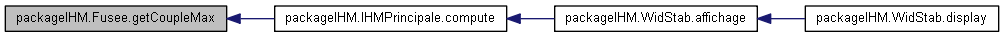
\includegraphics[width=350pt]{classpackage_i_h_m_1_1_fusee_a74a6a156b46d1fc48871201d4de59b00_icgraph}
\end{center}
\end{figure}
\mbox{\Hypertarget{classpackage_i_h_m_1_1_fusee_aa6f38f4cd95f564098a2f07535153e2e}\label{classpackage_i_h_m_1_1_fusee_aa6f38f4cd95f564098a2f07535153e2e}} 
\index{package\+I\+H\+M\+::\+Fusee@{package\+I\+H\+M\+::\+Fusee}!get\+Couple\+Min@{get\+Couple\+Min}}
\index{get\+Couple\+Min@{get\+Couple\+Min}!package\+I\+H\+M\+::\+Fusee@{package\+I\+H\+M\+::\+Fusee}}
\subsubsection{\texorpdfstring{get\+Couple\+Min()}{getCoupleMin()}}
{\footnotesize\ttfamily double package\+I\+H\+M.\+Fusee.\+get\+Couple\+Min (\begin{DoxyParamCaption}{ }\end{DoxyParamCaption})}

Here is the caller graph for this function\+:
\nopagebreak
\begin{figure}[H]
\begin{center}
\leavevmode
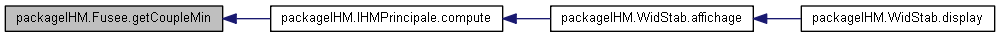
\includegraphics[width=350pt]{classpackage_i_h_m_1_1_fusee_aa6f38f4cd95f564098a2f07535153e2e_icgraph}
\end{center}
\end{figure}
\mbox{\Hypertarget{classpackage_i_h_m_1_1_fusee_ab62b66735d0bfcd293b916d21cf5e603}\label{classpackage_i_h_m_1_1_fusee_ab62b66735d0bfcd293b916d21cf5e603}} 
\index{package\+I\+H\+M\+::\+Fusee@{package\+I\+H\+M\+::\+Fusee}!get\+D2B@{get\+D2B}}
\index{get\+D2B@{get\+D2B}!package\+I\+H\+M\+::\+Fusee@{package\+I\+H\+M\+::\+Fusee}}
\subsubsection{\texorpdfstring{get\+D2\+B()}{getD2B()}}
{\footnotesize\ttfamily double package\+I\+H\+M.\+Fusee.\+get\+D2B (\begin{DoxyParamCaption}{ }\end{DoxyParamCaption})}

\mbox{\Hypertarget{classpackage_i_h_m_1_1_fusee_aba5822efc15396d0c978f71777cb187d}\label{classpackage_i_h_m_1_1_fusee_aba5822efc15396d0c978f71777cb187d}} 
\index{package\+I\+H\+M\+::\+Fusee@{package\+I\+H\+M\+::\+Fusee}!get\+Date\+Acceleration\+Maximale@{get\+Date\+Acceleration\+Maximale}}
\index{get\+Date\+Acceleration\+Maximale@{get\+Date\+Acceleration\+Maximale}!package\+I\+H\+M\+::\+Fusee@{package\+I\+H\+M\+::\+Fusee}}
\subsubsection{\texorpdfstring{get\+Date\+Acceleration\+Maximale()}{getDateAccelerationMaximale()}}
{\footnotesize\ttfamily double package\+I\+H\+M.\+Fusee.\+get\+Date\+Acceleration\+Maximale (\begin{DoxyParamCaption}{ }\end{DoxyParamCaption})}

\mbox{\Hypertarget{classpackage_i_h_m_1_1_fusee_a5e292a5c436c8a7d2325f41ca323e0ea}\label{classpackage_i_h_m_1_1_fusee_a5e292a5c436c8a7d2325f41ca323e0ea}} 
\index{package\+I\+H\+M\+::\+Fusee@{package\+I\+H\+M\+::\+Fusee}!get\+Date\+Vitesse\+Maximale@{get\+Date\+Vitesse\+Maximale}}
\index{get\+Date\+Vitesse\+Maximale@{get\+Date\+Vitesse\+Maximale}!package\+I\+H\+M\+::\+Fusee@{package\+I\+H\+M\+::\+Fusee}}
\subsubsection{\texorpdfstring{get\+Date\+Vitesse\+Maximale()}{getDateVitesseMaximale()}}
{\footnotesize\ttfamily double package\+I\+H\+M.\+Fusee.\+get\+Date\+Vitesse\+Maximale (\begin{DoxyParamCaption}{ }\end{DoxyParamCaption})}

\mbox{\Hypertarget{classpackage_i_h_m_1_1_fusee_ab693f7b8a6db9d4c7f112a4dd2d094ac}\label{classpackage_i_h_m_1_1_fusee_ab693f7b8a6db9d4c7f112a4dd2d094ac}} 
\index{package\+I\+H\+M\+::\+Fusee@{package\+I\+H\+M\+::\+Fusee}!get\+Duree\+Vol@{get\+Duree\+Vol}}
\index{get\+Duree\+Vol@{get\+Duree\+Vol}!package\+I\+H\+M\+::\+Fusee@{package\+I\+H\+M\+::\+Fusee}}
\subsubsection{\texorpdfstring{get\+Duree\+Vol()}{getDureeVol()}}
{\footnotesize\ttfamily double package\+I\+H\+M.\+Fusee.\+get\+Duree\+Vol (\begin{DoxyParamCaption}{ }\end{DoxyParamCaption})}

\mbox{\Hypertarget{classpackage_i_h_m_1_1_fusee_aae742d9537e9f3f6d72047927221b7cf}\label{classpackage_i_h_m_1_1_fusee_aae742d9537e9f3f6d72047927221b7cf}} 
\index{package\+I\+H\+M\+::\+Fusee@{package\+I\+H\+M\+::\+Fusee}!get\+Elancement@{get\+Elancement}}
\index{get\+Elancement@{get\+Elancement}!package\+I\+H\+M\+::\+Fusee@{package\+I\+H\+M\+::\+Fusee}}
\subsubsection{\texorpdfstring{get\+Elancement()}{getElancement()}}
{\footnotesize\ttfamily double package\+I\+H\+M.\+Fusee.\+get\+Elancement (\begin{DoxyParamCaption}{ }\end{DoxyParamCaption})}

Here is the caller graph for this function\+:
\nopagebreak
\begin{figure}[H]
\begin{center}
\leavevmode
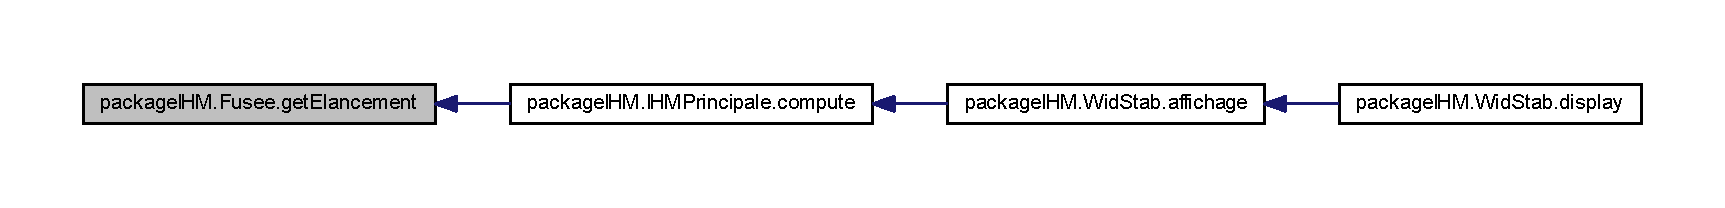
\includegraphics[width=350pt]{classpackage_i_h_m_1_1_fusee_aae742d9537e9f3f6d72047927221b7cf_icgraph}
\end{center}
\end{figure}
\mbox{\Hypertarget{classpackage_i_h_m_1_1_fusee_a1dc3db02b4bf99f6aca556ba0cee1694}\label{classpackage_i_h_m_1_1_fusee_a1dc3db02b4bf99f6aca556ba0cee1694}} 
\index{package\+I\+H\+M\+::\+Fusee@{package\+I\+H\+M\+::\+Fusee}!getf\+Ail@{getf\+Ail}}
\index{getf\+Ail@{getf\+Ail}!package\+I\+H\+M\+::\+Fusee@{package\+I\+H\+M\+::\+Fusee}}
\subsubsection{\texorpdfstring{getf\+Ail()}{getfAil()}}
{\footnotesize\ttfamily double package\+I\+H\+M.\+Fusee.\+getf\+Ail (\begin{DoxyParamCaption}{ }\end{DoxyParamCaption})}

\mbox{\Hypertarget{classpackage_i_h_m_1_1_fusee_ac1f22338847cdea9e2eb8460e816483e}\label{classpackage_i_h_m_1_1_fusee_ac1f22338847cdea9e2eb8460e816483e}} 
\index{package\+I\+H\+M\+::\+Fusee@{package\+I\+H\+M\+::\+Fusee}!getf\+Can@{getf\+Can}}
\index{getf\+Can@{getf\+Can}!package\+I\+H\+M\+::\+Fusee@{package\+I\+H\+M\+::\+Fusee}}
\subsubsection{\texorpdfstring{getf\+Can()}{getfCan()}}
{\footnotesize\ttfamily double package\+I\+H\+M.\+Fusee.\+getf\+Can (\begin{DoxyParamCaption}{ }\end{DoxyParamCaption})}

\mbox{\Hypertarget{classpackage_i_h_m_1_1_fusee_a5dc3253e6bcfb9f7c3d8de5db1ad9626}\label{classpackage_i_h_m_1_1_fusee_a5dc3253e6bcfb9f7c3d8de5db1ad9626}} 
\index{package\+I\+H\+M\+::\+Fusee@{package\+I\+H\+M\+::\+Fusee}!getf\+Masq@{getf\+Masq}}
\index{getf\+Masq@{getf\+Masq}!package\+I\+H\+M\+::\+Fusee@{package\+I\+H\+M\+::\+Fusee}}
\subsubsection{\texorpdfstring{getf\+Masq()}{getfMasq()}}
{\footnotesize\ttfamily double package\+I\+H\+M.\+Fusee.\+getf\+Masq (\begin{DoxyParamCaption}{ }\end{DoxyParamCaption})}

\mbox{\Hypertarget{classpackage_i_h_m_1_1_fusee_afca23d0b33bc1a464157c41089d0dd64}\label{classpackage_i_h_m_1_1_fusee_afca23d0b33bc1a464157c41089d0dd64}} 
\index{package\+I\+H\+M\+::\+Fusee@{package\+I\+H\+M\+::\+Fusee}!get\+Long\+Tot@{get\+Long\+Tot}}
\index{get\+Long\+Tot@{get\+Long\+Tot}!package\+I\+H\+M\+::\+Fusee@{package\+I\+H\+M\+::\+Fusee}}
\subsubsection{\texorpdfstring{get\+Long\+Tot()}{getLongTot()}}
{\footnotesize\ttfamily double package\+I\+H\+M.\+Fusee.\+get\+Long\+Tot (\begin{DoxyParamCaption}{ }\end{DoxyParamCaption})}

\mbox{\Hypertarget{classpackage_i_h_m_1_1_fusee_a4764587470f7deab8f4738bea5ecf067}\label{classpackage_i_h_m_1_1_fusee_a4764587470f7deab8f4738bea5ecf067}} 
\index{package\+I\+H\+M\+::\+Fusee@{package\+I\+H\+M\+::\+Fusee}!get\+Mach\+\_\+max@{get\+Mach\+\_\+max}}
\index{get\+Mach\+\_\+max@{get\+Mach\+\_\+max}!package\+I\+H\+M\+::\+Fusee@{package\+I\+H\+M\+::\+Fusee}}
\subsubsection{\texorpdfstring{get\+Mach\+\_\+max()}{getMach\_max()}}
{\footnotesize\ttfamily double package\+I\+H\+M.\+Fusee.\+get\+Mach\+\_\+max (\begin{DoxyParamCaption}{ }\end{DoxyParamCaption})}

\mbox{\Hypertarget{classpackage_i_h_m_1_1_fusee_a28633a472bfd8c406c8c6d0b53dab006}\label{classpackage_i_h_m_1_1_fusee_a28633a472bfd8c406c8c6d0b53dab006}} 
\index{package\+I\+H\+M\+::\+Fusee@{package\+I\+H\+M\+::\+Fusee}!get\+Masse\+Para@{get\+Masse\+Para}}
\index{get\+Masse\+Para@{get\+Masse\+Para}!package\+I\+H\+M\+::\+Fusee@{package\+I\+H\+M\+::\+Fusee}}
\subsubsection{\texorpdfstring{get\+Masse\+Para()}{getMassePara()}}
{\footnotesize\ttfamily double package\+I\+H\+M.\+Fusee.\+get\+Masse\+Para (\begin{DoxyParamCaption}{ }\end{DoxyParamCaption})}

Here is the caller graph for this function\+:
\nopagebreak
\begin{figure}[H]
\begin{center}
\leavevmode
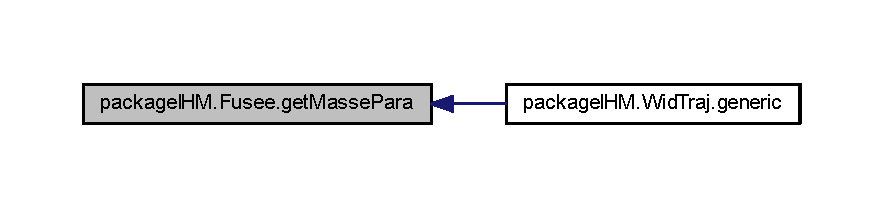
\includegraphics[width=350pt]{classpackage_i_h_m_1_1_fusee_a28633a472bfd8c406c8c6d0b53dab006_icgraph}
\end{center}
\end{figure}
\mbox{\Hypertarget{classpackage_i_h_m_1_1_fusee_a14ed536736006c6483135f0356b7f24a}\label{classpackage_i_h_m_1_1_fusee_a14ed536736006c6483135f0356b7f24a}} 
\index{package\+I\+H\+M\+::\+Fusee@{package\+I\+H\+M\+::\+Fusee}!get\+Masse\+Plein@{get\+Masse\+Plein}}
\index{get\+Masse\+Plein@{get\+Masse\+Plein}!package\+I\+H\+M\+::\+Fusee@{package\+I\+H\+M\+::\+Fusee}}
\subsubsection{\texorpdfstring{get\+Masse\+Plein()}{getMassePlein()}}
{\footnotesize\ttfamily double package\+I\+H\+M.\+Fusee.\+get\+Masse\+Plein (\begin{DoxyParamCaption}{ }\end{DoxyParamCaption})}

Here is the caller graph for this function\+:
\nopagebreak
\begin{figure}[H]
\begin{center}
\leavevmode
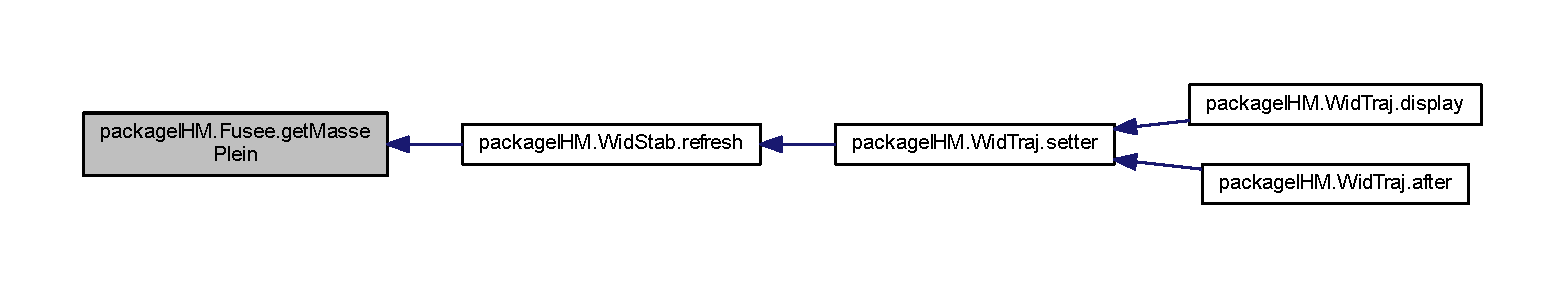
\includegraphics[width=350pt]{classpackage_i_h_m_1_1_fusee_a14ed536736006c6483135f0356b7f24a_icgraph}
\end{center}
\end{figure}
\mbox{\Hypertarget{classpackage_i_h_m_1_1_fusee_a041b9744320e9542be57dc3213090695}\label{classpackage_i_h_m_1_1_fusee_a041b9744320e9542be57dc3213090695}} 
\index{package\+I\+H\+M\+::\+Fusee@{package\+I\+H\+M\+::\+Fusee}!get\+Masse\+Sans\+Moteur@{get\+Masse\+Sans\+Moteur}}
\index{get\+Masse\+Sans\+Moteur@{get\+Masse\+Sans\+Moteur}!package\+I\+H\+M\+::\+Fusee@{package\+I\+H\+M\+::\+Fusee}}
\subsubsection{\texorpdfstring{get\+Masse\+Sans\+Moteur()}{getMasseSansMoteur()}}
{\footnotesize\ttfamily double package\+I\+H\+M.\+Fusee.\+get\+Masse\+Sans\+Moteur (\begin{DoxyParamCaption}{ }\end{DoxyParamCaption})}

Getters of the input data of the trajectory Here is the caller graph for this function\+:
\nopagebreak
\begin{figure}[H]
\begin{center}
\leavevmode
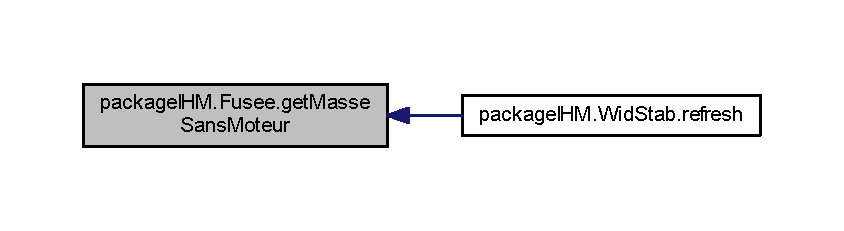
\includegraphics[width=350pt]{classpackage_i_h_m_1_1_fusee_a041b9744320e9542be57dc3213090695_icgraph}
\end{center}
\end{figure}
\mbox{\Hypertarget{classpackage_i_h_m_1_1_fusee_ad951fb65e362de81a51886a313b5eccb}\label{classpackage_i_h_m_1_1_fusee_ad951fb65e362de81a51886a313b5eccb}} 
\index{package\+I\+H\+M\+::\+Fusee@{package\+I\+H\+M\+::\+Fusee}!get\+Masse\+Vide@{get\+Masse\+Vide}}
\index{get\+Masse\+Vide@{get\+Masse\+Vide}!package\+I\+H\+M\+::\+Fusee@{package\+I\+H\+M\+::\+Fusee}}
\subsubsection{\texorpdfstring{get\+Masse\+Vide()}{getMasseVide()}}
{\footnotesize\ttfamily double package\+I\+H\+M.\+Fusee.\+get\+Masse\+Vide (\begin{DoxyParamCaption}{ }\end{DoxyParamCaption})}

Here is the caller graph for this function\+:
\nopagebreak
\begin{figure}[H]
\begin{center}
\leavevmode
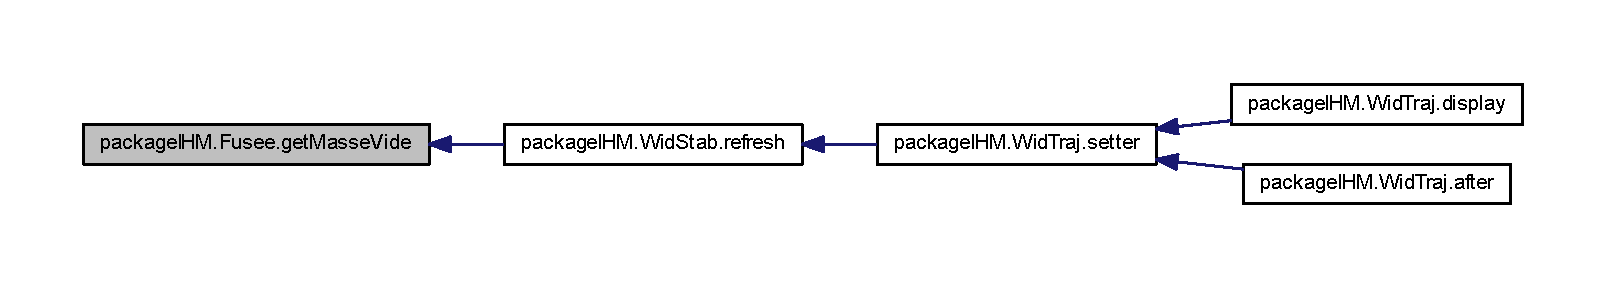
\includegraphics[width=350pt]{classpackage_i_h_m_1_1_fusee_ad951fb65e362de81a51886a313b5eccb_icgraph}
\end{center}
\end{figure}
\mbox{\Hypertarget{classpackage_i_h_m_1_1_fusee_ac4f58a623e42fa4674dcc3b96c4eecc0}\label{classpackage_i_h_m_1_1_fusee_ac4f58a623e42fa4674dcc3b96c4eecc0}} 
\index{package\+I\+H\+M\+::\+Fusee@{package\+I\+H\+M\+::\+Fusee}!get\+M\+S\+Max@{get\+M\+S\+Max}}
\index{get\+M\+S\+Max@{get\+M\+S\+Max}!package\+I\+H\+M\+::\+Fusee@{package\+I\+H\+M\+::\+Fusee}}
\subsubsection{\texorpdfstring{get\+M\+S\+Max()}{getMSMax()}}
{\footnotesize\ttfamily double package\+I\+H\+M.\+Fusee.\+get\+M\+S\+Max (\begin{DoxyParamCaption}{ }\end{DoxyParamCaption})}

Here is the caller graph for this function\+:
\nopagebreak
\begin{figure}[H]
\begin{center}
\leavevmode
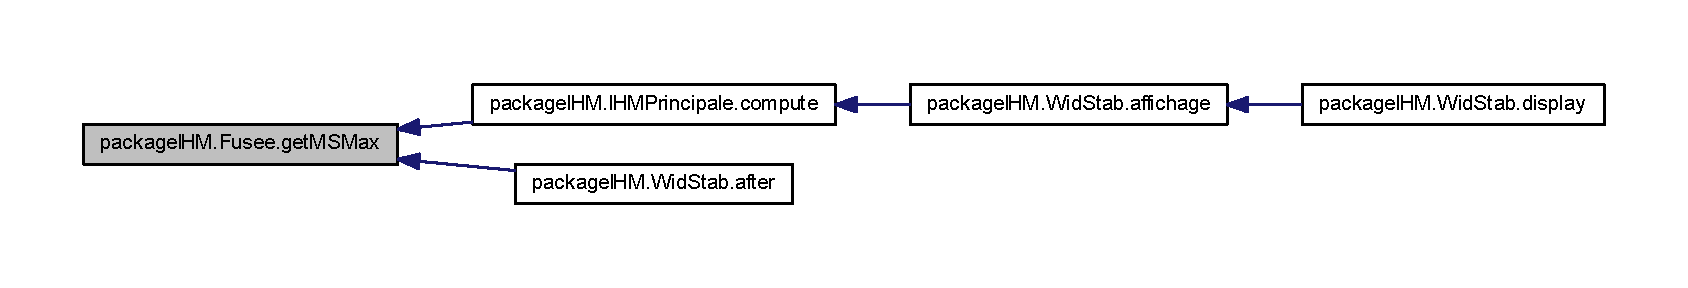
\includegraphics[width=350pt]{classpackage_i_h_m_1_1_fusee_ac4f58a623e42fa4674dcc3b96c4eecc0_icgraph}
\end{center}
\end{figure}
\mbox{\Hypertarget{classpackage_i_h_m_1_1_fusee_a91878f710e3a177f75f242c2e8a0a129}\label{classpackage_i_h_m_1_1_fusee_a91878f710e3a177f75f242c2e8a0a129}} 
\index{package\+I\+H\+M\+::\+Fusee@{package\+I\+H\+M\+::\+Fusee}!get\+M\+S\+Min@{get\+M\+S\+Min}}
\index{get\+M\+S\+Min@{get\+M\+S\+Min}!package\+I\+H\+M\+::\+Fusee@{package\+I\+H\+M\+::\+Fusee}}
\subsubsection{\texorpdfstring{get\+M\+S\+Min()}{getMSMin()}}
{\footnotesize\ttfamily double package\+I\+H\+M.\+Fusee.\+get\+M\+S\+Min (\begin{DoxyParamCaption}{ }\end{DoxyParamCaption})}

Here is the caller graph for this function\+:
\nopagebreak
\begin{figure}[H]
\begin{center}
\leavevmode
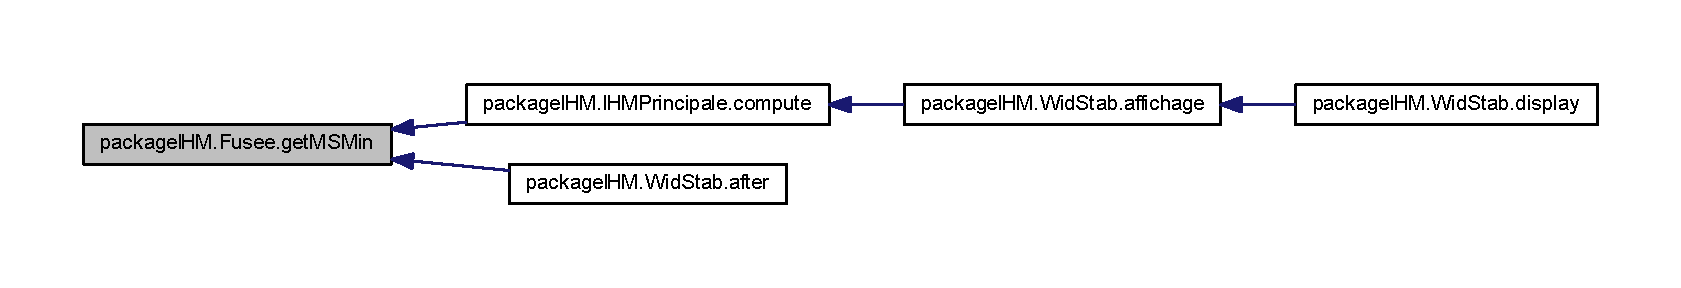
\includegraphics[width=350pt]{classpackage_i_h_m_1_1_fusee_a91878f710e3a177f75f242c2e8a0a129_icgraph}
\end{center}
\end{figure}
\mbox{\Hypertarget{classpackage_i_h_m_1_1_fusee_afc0492c0c663001bd7a0369842e988ba}\label{classpackage_i_h_m_1_1_fusee_afc0492c0c663001bd7a0369842e988ba}} 
\index{package\+I\+H\+M\+::\+Fusee@{package\+I\+H\+M\+::\+Fusee}!get\+Portance\+Fusee@{get\+Portance\+Fusee}}
\index{get\+Portance\+Fusee@{get\+Portance\+Fusee}!package\+I\+H\+M\+::\+Fusee@{package\+I\+H\+M\+::\+Fusee}}
\subsubsection{\texorpdfstring{get\+Portance\+Fusee()}{getPortanceFusee()}}
{\footnotesize\ttfamily double package\+I\+H\+M.\+Fusee.\+get\+Portance\+Fusee (\begin{DoxyParamCaption}{ }\end{DoxyParamCaption})}

Getters of the input data of the stability Getters of the output data of the stability Here is the caller graph for this function\+:
\nopagebreak
\begin{figure}[H]
\begin{center}
\leavevmode
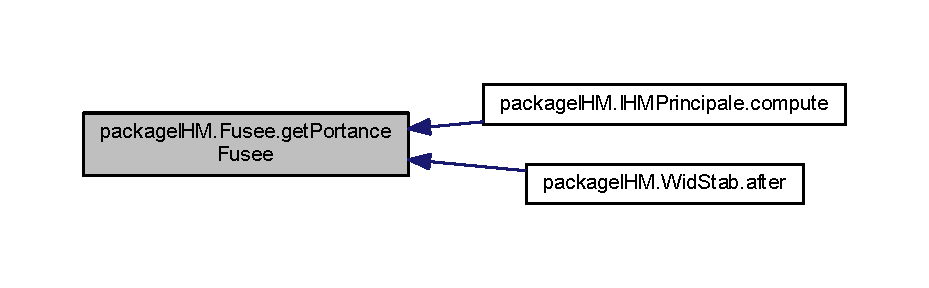
\includegraphics[width=350pt]{classpackage_i_h_m_1_1_fusee_afc0492c0c663001bd7a0369842e988ba_icgraph}
\end{center}
\end{figure}
\mbox{\Hypertarget{classpackage_i_h_m_1_1_fusee_ae9bc0685a063a007055f8395aacb3b2a}\label{classpackage_i_h_m_1_1_fusee_ae9bc0685a063a007055f8395aacb3b2a}} 
\index{package\+I\+H\+M\+::\+Fusee@{package\+I\+H\+M\+::\+Fusee}!get\+Portee\+Balistique@{get\+Portee\+Balistique}}
\index{get\+Portee\+Balistique@{get\+Portee\+Balistique}!package\+I\+H\+M\+::\+Fusee@{package\+I\+H\+M\+::\+Fusee}}
\subsubsection{\texorpdfstring{get\+Portee\+Balistique()}{getPorteeBalistique()}}
{\footnotesize\ttfamily double package\+I\+H\+M.\+Fusee.\+get\+Portee\+Balistique (\begin{DoxyParamCaption}{ }\end{DoxyParamCaption})}

\mbox{\Hypertarget{classpackage_i_h_m_1_1_fusee_a86af3645420069b63f9ebfdae4ec7895}\label{classpackage_i_h_m_1_1_fusee_a86af3645420069b63f9ebfdae4ec7895}} 
\index{package\+I\+H\+M\+::\+Fusee@{package\+I\+H\+M\+::\+Fusee}!get\+S\+Ref\+Trainee@{get\+S\+Ref\+Trainee}}
\index{get\+S\+Ref\+Trainee@{get\+S\+Ref\+Trainee}!package\+I\+H\+M\+::\+Fusee@{package\+I\+H\+M\+::\+Fusee}}
\subsubsection{\texorpdfstring{get\+S\+Ref\+Trainee()}{getSRefTrainee()}}
{\footnotesize\ttfamily double package\+I\+H\+M.\+Fusee.\+get\+S\+Ref\+Trainee (\begin{DoxyParamCaption}{ }\end{DoxyParamCaption})}

Getters of the output data of the trajectory Here is the caller graph for this function\+:
\nopagebreak
\begin{figure}[H]
\begin{center}
\leavevmode
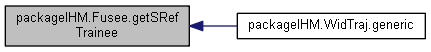
\includegraphics[width=350pt]{classpackage_i_h_m_1_1_fusee_a86af3645420069b63f9ebfdae4ec7895_icgraph}
\end{center}
\end{figure}
\mbox{\Hypertarget{classpackage_i_h_m_1_1_fusee_a262179da88718476dfa7f9085aed44bf}\label{classpackage_i_h_m_1_1_fusee_a262179da88718476dfa7f9085aed44bf}} 
\index{package\+I\+H\+M\+::\+Fusee@{package\+I\+H\+M\+::\+Fusee}!get\+Temps\+Culmination@{get\+Temps\+Culmination}}
\index{get\+Temps\+Culmination@{get\+Temps\+Culmination}!package\+I\+H\+M\+::\+Fusee@{package\+I\+H\+M\+::\+Fusee}}
\subsubsection{\texorpdfstring{get\+Temps\+Culmination()}{getTempsCulmination()}}
{\footnotesize\ttfamily double package\+I\+H\+M.\+Fusee.\+get\+Temps\+Culmination (\begin{DoxyParamCaption}{ }\end{DoxyParamCaption})}

\mbox{\Hypertarget{classpackage_i_h_m_1_1_fusee_ab5ef8a4e7e00ede675f2b8ed78e30505}\label{classpackage_i_h_m_1_1_fusee_ab5ef8a4e7e00ede675f2b8ed78e30505}} 
\index{package\+I\+H\+M\+::\+Fusee@{package\+I\+H\+M\+::\+Fusee}!get\+Temps\+Fin\+Prop@{get\+Temps\+Fin\+Prop}}
\index{get\+Temps\+Fin\+Prop@{get\+Temps\+Fin\+Prop}!package\+I\+H\+M\+::\+Fusee@{package\+I\+H\+M\+::\+Fusee}}
\subsubsection{\texorpdfstring{get\+Temps\+Fin\+Prop()}{getTempsFinProp()}}
{\footnotesize\ttfamily double package\+I\+H\+M.\+Fusee.\+get\+Temps\+Fin\+Prop (\begin{DoxyParamCaption}{ }\end{DoxyParamCaption})}

\mbox{\Hypertarget{classpackage_i_h_m_1_1_fusee_a95ff15476f93d411cf04fca67f6756b2}\label{classpackage_i_h_m_1_1_fusee_a95ff15476f93d411cf04fca67f6756b2}} 
\index{package\+I\+H\+M\+::\+Fusee@{package\+I\+H\+M\+::\+Fusee}!get\+Vitesse\+Culmination@{get\+Vitesse\+Culmination}}
\index{get\+Vitesse\+Culmination@{get\+Vitesse\+Culmination}!package\+I\+H\+M\+::\+Fusee@{package\+I\+H\+M\+::\+Fusee}}
\subsubsection{\texorpdfstring{get\+Vitesse\+Culmination()}{getVitesseCulmination()}}
{\footnotesize\ttfamily double package\+I\+H\+M.\+Fusee.\+get\+Vitesse\+Culmination (\begin{DoxyParamCaption}{ }\end{DoxyParamCaption})}

\mbox{\Hypertarget{classpackage_i_h_m_1_1_fusee_a8bee21c341bae021f584ad310b0ff69f}\label{classpackage_i_h_m_1_1_fusee_a8bee21c341bae021f584ad310b0ff69f}} 
\index{package\+I\+H\+M\+::\+Fusee@{package\+I\+H\+M\+::\+Fusee}!get\+Vitesse\+Sortie\+Rampe@{get\+Vitesse\+Sortie\+Rampe}}
\index{get\+Vitesse\+Sortie\+Rampe@{get\+Vitesse\+Sortie\+Rampe}!package\+I\+H\+M\+::\+Fusee@{package\+I\+H\+M\+::\+Fusee}}
\subsubsection{\texorpdfstring{get\+Vitesse\+Sortie\+Rampe()}{getVitesseSortieRampe()}}
{\footnotesize\ttfamily double package\+I\+H\+M.\+Fusee.\+get\+Vitesse\+Sortie\+Rampe (\begin{DoxyParamCaption}{ }\end{DoxyParamCaption})}

\mbox{\Hypertarget{classpackage_i_h_m_1_1_fusee_ac461ab2a6086285d105ff579f98ffe80}\label{classpackage_i_h_m_1_1_fusee_ac461ab2a6086285d105ff579f98ffe80}} 
\index{package\+I\+H\+M\+::\+Fusee@{package\+I\+H\+M\+::\+Fusee}!get\+V\+Para@{get\+V\+Para}}
\index{get\+V\+Para@{get\+V\+Para}!package\+I\+H\+M\+::\+Fusee@{package\+I\+H\+M\+::\+Fusee}}
\subsubsection{\texorpdfstring{get\+V\+Para()}{getVPara()}}
{\footnotesize\ttfamily double package\+I\+H\+M.\+Fusee.\+get\+V\+Para (\begin{DoxyParamCaption}{ }\end{DoxyParamCaption})}

Here is the caller graph for this function\+:
\nopagebreak
\begin{figure}[H]
\begin{center}
\leavevmode
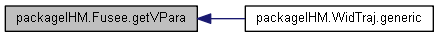
\includegraphics[width=350pt]{classpackage_i_h_m_1_1_fusee_ac461ab2a6086285d105ff579f98ffe80_icgraph}
\end{center}
\end{figure}
\mbox{\Hypertarget{classpackage_i_h_m_1_1_fusee_a02bc51e970a959aeff2c9b05cce2c564}\label{classpackage_i_h_m_1_1_fusee_a02bc51e970a959aeff2c9b05cce2c564}} 
\index{package\+I\+H\+M\+::\+Fusee@{package\+I\+H\+M\+::\+Fusee}!get\+V\+Para1@{get\+V\+Para1}}
\index{get\+V\+Para1@{get\+V\+Para1}!package\+I\+H\+M\+::\+Fusee@{package\+I\+H\+M\+::\+Fusee}}
\subsubsection{\texorpdfstring{get\+V\+Para1()}{getVPara1()}}
{\footnotesize\ttfamily double package\+I\+H\+M.\+Fusee.\+get\+V\+Para1 (\begin{DoxyParamCaption}{ }\end{DoxyParamCaption})}

Here is the caller graph for this function\+:
\nopagebreak
\begin{figure}[H]
\begin{center}
\leavevmode
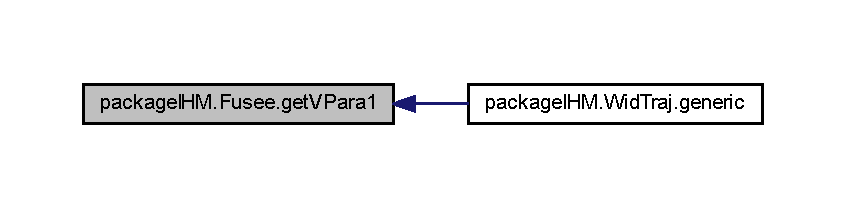
\includegraphics[width=350pt]{classpackage_i_h_m_1_1_fusee_a02bc51e970a959aeff2c9b05cce2c564_icgraph}
\end{center}
\end{figure}
\mbox{\Hypertarget{classpackage_i_h_m_1_1_fusee_a92c7ba71a122f2b8d528a097fc0ef6e0}\label{classpackage_i_h_m_1_1_fusee_a92c7ba71a122f2b8d528a097fc0ef6e0}} 
\index{package\+I\+H\+M\+::\+Fusee@{package\+I\+H\+M\+::\+Fusee}!get\+V\+Para2@{get\+V\+Para2}}
\index{get\+V\+Para2@{get\+V\+Para2}!package\+I\+H\+M\+::\+Fusee@{package\+I\+H\+M\+::\+Fusee}}
\subsubsection{\texorpdfstring{get\+V\+Para2()}{getVPara2()}}
{\footnotesize\ttfamily double package\+I\+H\+M.\+Fusee.\+get\+V\+Para2 (\begin{DoxyParamCaption}{ }\end{DoxyParamCaption})}

Here is the caller graph for this function\+:
\nopagebreak
\begin{figure}[H]
\begin{center}
\leavevmode
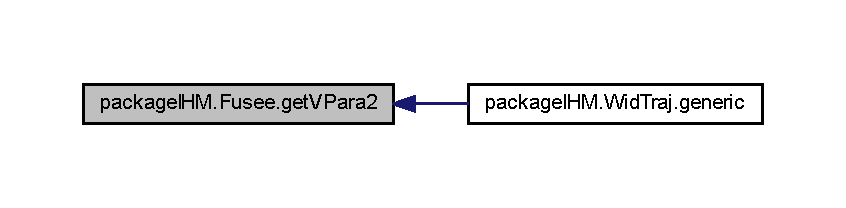
\includegraphics[width=350pt]{classpackage_i_h_m_1_1_fusee_a92c7ba71a122f2b8d528a097fc0ef6e0_icgraph}
\end{center}
\end{figure}
\mbox{\Hypertarget{classpackage_i_h_m_1_1_fusee_a63fd0c6ecd18920dddc6d921d8e2e756}\label{classpackage_i_h_m_1_1_fusee_a63fd0c6ecd18920dddc6d921d8e2e756}} 
\index{package\+I\+H\+M\+::\+Fusee@{package\+I\+H\+M\+::\+Fusee}!get\+X\+C\+G\+Plein@{get\+X\+C\+G\+Plein}}
\index{get\+X\+C\+G\+Plein@{get\+X\+C\+G\+Plein}!package\+I\+H\+M\+::\+Fusee@{package\+I\+H\+M\+::\+Fusee}}
\subsubsection{\texorpdfstring{get\+X\+C\+G\+Plein()}{getXCGPlein()}}
{\footnotesize\ttfamily double package\+I\+H\+M.\+Fusee.\+get\+X\+C\+G\+Plein (\begin{DoxyParamCaption}{ }\end{DoxyParamCaption})}

Here is the caller graph for this function\+:
\nopagebreak
\begin{figure}[H]
\begin{center}
\leavevmode
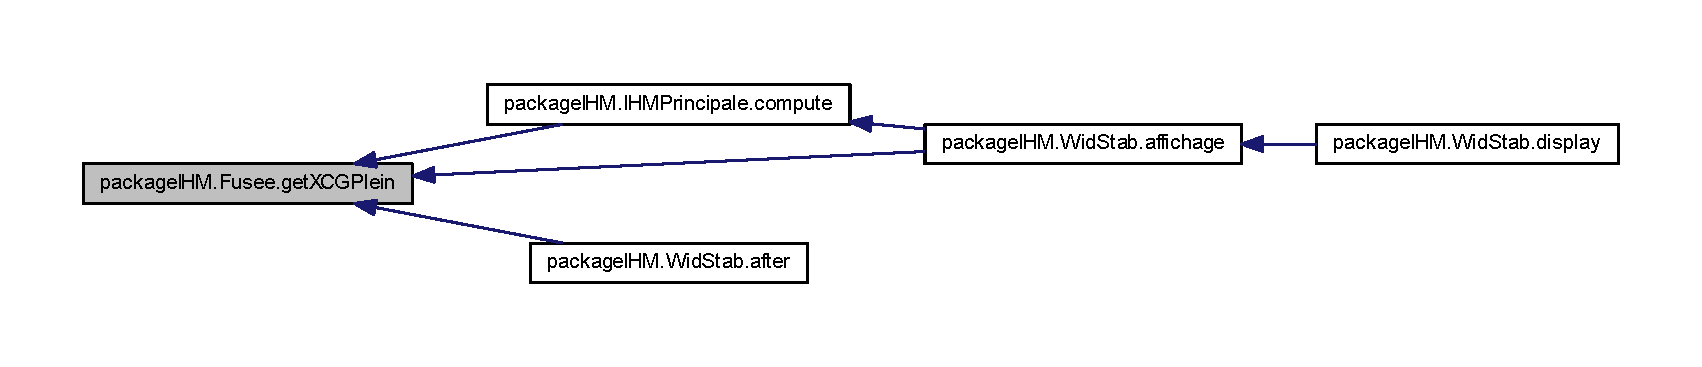
\includegraphics[width=350pt]{classpackage_i_h_m_1_1_fusee_a63fd0c6ecd18920dddc6d921d8e2e756_icgraph}
\end{center}
\end{figure}
\mbox{\Hypertarget{classpackage_i_h_m_1_1_fusee_a0ff2feb9e773be035788c1ad77bcb4b9}\label{classpackage_i_h_m_1_1_fusee_a0ff2feb9e773be035788c1ad77bcb4b9}} 
\index{package\+I\+H\+M\+::\+Fusee@{package\+I\+H\+M\+::\+Fusee}!get\+X\+C\+G\+Vide@{get\+X\+C\+G\+Vide}}
\index{get\+X\+C\+G\+Vide@{get\+X\+C\+G\+Vide}!package\+I\+H\+M\+::\+Fusee@{package\+I\+H\+M\+::\+Fusee}}
\subsubsection{\texorpdfstring{get\+X\+C\+G\+Vide()}{getXCGVide()}}
{\footnotesize\ttfamily double package\+I\+H\+M.\+Fusee.\+get\+X\+C\+G\+Vide (\begin{DoxyParamCaption}{ }\end{DoxyParamCaption})}

Here is the caller graph for this function\+:
\nopagebreak
\begin{figure}[H]
\begin{center}
\leavevmode
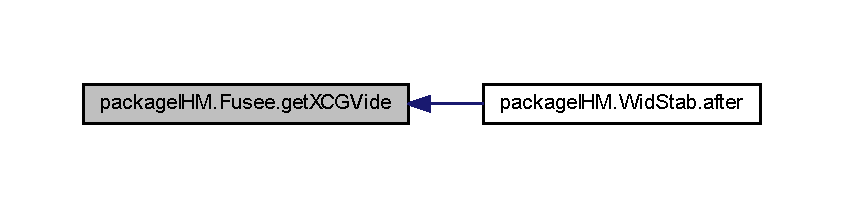
\includegraphics[width=350pt]{classpackage_i_h_m_1_1_fusee_a0ff2feb9e773be035788c1ad77bcb4b9_icgraph}
\end{center}
\end{figure}
\mbox{\Hypertarget{classpackage_i_h_m_1_1_fusee_a293775dd64424e3141abf1dac202ed30}\label{classpackage_i_h_m_1_1_fusee_a293775dd64424e3141abf1dac202ed30}} 
\index{package\+I\+H\+M\+::\+Fusee@{package\+I\+H\+M\+::\+Fusee}!get\+X\+C\+P\+Fusee@{get\+X\+C\+P\+Fusee}}
\index{get\+X\+C\+P\+Fusee@{get\+X\+C\+P\+Fusee}!package\+I\+H\+M\+::\+Fusee@{package\+I\+H\+M\+::\+Fusee}}
\subsubsection{\texorpdfstring{get\+X\+C\+P\+Fusee()}{getXCPFusee()}}
{\footnotesize\ttfamily double package\+I\+H\+M.\+Fusee.\+get\+X\+C\+P\+Fusee (\begin{DoxyParamCaption}{ }\end{DoxyParamCaption})}

Here is the caller graph for this function\+:
\nopagebreak
\begin{figure}[H]
\begin{center}
\leavevmode
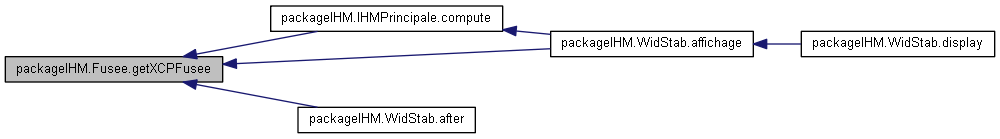
\includegraphics[width=350pt]{classpackage_i_h_m_1_1_fusee_a293775dd64424e3141abf1dac202ed30_icgraph}
\end{center}
\end{figure}
\mbox{\Hypertarget{classpackage_i_h_m_1_1_fusee_a6184007212fa89f33da93d80d703350e}\label{classpackage_i_h_m_1_1_fusee_a6184007212fa89f33da93d80d703350e}} 
\index{package\+I\+H\+M\+::\+Fusee@{package\+I\+H\+M\+::\+Fusee}!set\+Acceleration\+Maximale@{set\+Acceleration\+Maximale}}
\index{set\+Acceleration\+Maximale@{set\+Acceleration\+Maximale}!package\+I\+H\+M\+::\+Fusee@{package\+I\+H\+M\+::\+Fusee}}
\subsubsection{\texorpdfstring{set\+Acceleration\+Maximale()}{setAccelerationMaximale()}}
{\footnotesize\ttfamily void package\+I\+H\+M.\+Fusee.\+set\+Acceleration\+Maximale (\begin{DoxyParamCaption}\item[{double}]{p\+Acceleration\+Maximale }\end{DoxyParamCaption})}

\mbox{\Hypertarget{classpackage_i_h_m_1_1_fusee_afc465cf007d83a12e39f9c6d6480c598}\label{classpackage_i_h_m_1_1_fusee_afc465cf007d83a12e39f9c6d6480c598}} 
\index{package\+I\+H\+M\+::\+Fusee@{package\+I\+H\+M\+::\+Fusee}!set\+Acc\+Max@{set\+Acc\+Max}}
\index{set\+Acc\+Max@{set\+Acc\+Max}!package\+I\+H\+M\+::\+Fusee@{package\+I\+H\+M\+::\+Fusee}}
\subsubsection{\texorpdfstring{set\+Acc\+Max()}{setAccMax()}}
{\footnotesize\ttfamily void package\+I\+H\+M.\+Fusee.\+set\+Acc\+Max (\begin{DoxyParamCaption}\item[{double}]{p\+Acc\+Max }\end{DoxyParamCaption})}

\mbox{\Hypertarget{classpackage_i_h_m_1_1_fusee_a267ec95b3ae1a0746cb8f44f3fa7492c}\label{classpackage_i_h_m_1_1_fusee_a267ec95b3ae1a0746cb8f44f3fa7492c}} 
\index{package\+I\+H\+M\+::\+Fusee@{package\+I\+H\+M\+::\+Fusee}!set\+Alt\+Culmination@{set\+Alt\+Culmination}}
\index{set\+Alt\+Culmination@{set\+Alt\+Culmination}!package\+I\+H\+M\+::\+Fusee@{package\+I\+H\+M\+::\+Fusee}}
\subsubsection{\texorpdfstring{set\+Alt\+Culmination()}{setAltCulmination()}}
{\footnotesize\ttfamily void package\+I\+H\+M.\+Fusee.\+set\+Alt\+Culmination (\begin{DoxyParamCaption}\item[{double}]{p\+Alt\+Culmination }\end{DoxyParamCaption})}

Setters of the output data of the trajectory \mbox{\Hypertarget{classpackage_i_h_m_1_1_fusee_a96839656a0cb81be493e3ef2a1af2302}\label{classpackage_i_h_m_1_1_fusee_a96839656a0cb81be493e3ef2a1af2302}} 
\index{package\+I\+H\+M\+::\+Fusee@{package\+I\+H\+M\+::\+Fusee}!set\+Altitude\+Culmination@{set\+Altitude\+Culmination}}
\index{set\+Altitude\+Culmination@{set\+Altitude\+Culmination}!package\+I\+H\+M\+::\+Fusee@{package\+I\+H\+M\+::\+Fusee}}
\subsubsection{\texorpdfstring{set\+Altitude\+Culmination()}{setAltitudeCulmination()}}
{\footnotesize\ttfamily void package\+I\+H\+M.\+Fusee.\+set\+Altitude\+Culmination (\begin{DoxyParamCaption}\item[{double}]{p\+Altitude\+Culmination }\end{DoxyParamCaption})}

\mbox{\Hypertarget{classpackage_i_h_m_1_1_fusee_a9194203543c28c7c50b1a029d12dd784}\label{classpackage_i_h_m_1_1_fusee_a9194203543c28c7c50b1a029d12dd784}} 
\index{package\+I\+H\+M\+::\+Fusee@{package\+I\+H\+M\+::\+Fusee}!set\+Alt\+Para@{set\+Alt\+Para}}
\index{set\+Alt\+Para@{set\+Alt\+Para}!package\+I\+H\+M\+::\+Fusee@{package\+I\+H\+M\+::\+Fusee}}
\subsubsection{\texorpdfstring{set\+Alt\+Para()}{setAltPara()}}
{\footnotesize\ttfamily void package\+I\+H\+M.\+Fusee.\+set\+Alt\+Para (\begin{DoxyParamCaption}\item[{double}]{p\+Alt\+Para }\end{DoxyParamCaption})}

\mbox{\Hypertarget{classpackage_i_h_m_1_1_fusee_a32d41073cc48f50691b7b4963a9c1d59}\label{classpackage_i_h_m_1_1_fusee_a32d41073cc48f50691b7b4963a9c1d59}} 
\index{package\+I\+H\+M\+::\+Fusee@{package\+I\+H\+M\+::\+Fusee}!set\+Alt\+Rampe@{set\+Alt\+Rampe}}
\index{set\+Alt\+Rampe@{set\+Alt\+Rampe}!package\+I\+H\+M\+::\+Fusee@{package\+I\+H\+M\+::\+Fusee}}
\subsubsection{\texorpdfstring{set\+Alt\+Rampe()}{setAltRampe()}}
{\footnotesize\ttfamily void package\+I\+H\+M.\+Fusee.\+set\+Alt\+Rampe (\begin{DoxyParamCaption}\item[{double}]{p\+Alt\+Rampe }\end{DoxyParamCaption})}

Here is the caller graph for this function\+:
\nopagebreak
\begin{figure}[H]
\begin{center}
\leavevmode
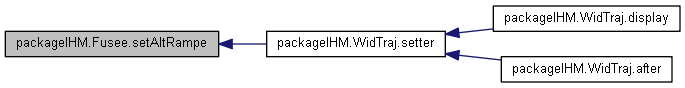
\includegraphics[width=350pt]{classpackage_i_h_m_1_1_fusee_a32d41073cc48f50691b7b4963a9c1d59_icgraph}
\end{center}
\end{figure}
\mbox{\Hypertarget{classpackage_i_h_m_1_1_fusee_a4cad2736b162ca0f3fdca9a469636b15}\label{classpackage_i_h_m_1_1_fusee_a4cad2736b162ca0f3fdca9a469636b15}} 
\index{package\+I\+H\+M\+::\+Fusee@{package\+I\+H\+M\+::\+Fusee}!set\+Beta\+Rampe@{set\+Beta\+Rampe}}
\index{set\+Beta\+Rampe@{set\+Beta\+Rampe}!package\+I\+H\+M\+::\+Fusee@{package\+I\+H\+M\+::\+Fusee}}
\subsubsection{\texorpdfstring{set\+Beta\+Rampe()}{setBetaRampe()}}
{\footnotesize\ttfamily void package\+I\+H\+M.\+Fusee.\+set\+Beta\+Rampe (\begin{DoxyParamCaption}\item[{double}]{p\+Beta\+Rampe }\end{DoxyParamCaption})}

Here is the caller graph for this function\+:
\nopagebreak
\begin{figure}[H]
\begin{center}
\leavevmode
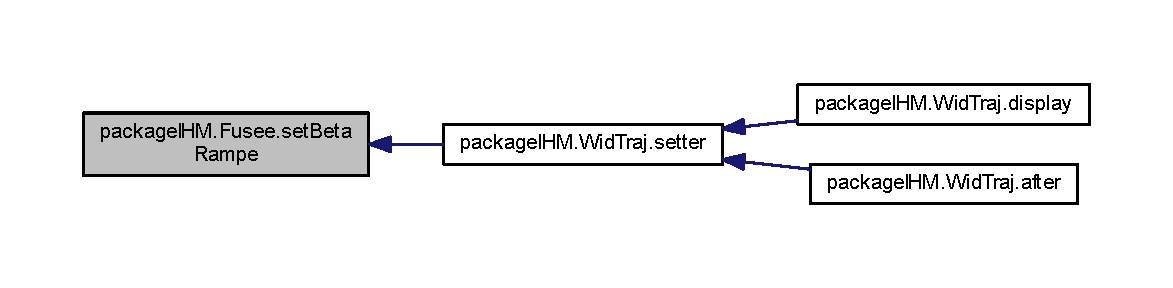
\includegraphics[width=350pt]{classpackage_i_h_m_1_1_fusee_a4cad2736b162ca0f3fdca9a469636b15_icgraph}
\end{center}
\end{figure}
\mbox{\Hypertarget{classpackage_i_h_m_1_1_fusee_acbae8e0b1ab85bd7ef477c21093d829b}\label{classpackage_i_h_m_1_1_fusee_acbae8e0b1ab85bd7ef477c21093d829b}} 
\index{package\+I\+H\+M\+::\+Fusee@{package\+I\+H\+M\+::\+Fusee}!set\+Choix\+Depotage@{set\+Choix\+Depotage}}
\index{set\+Choix\+Depotage@{set\+Choix\+Depotage}!package\+I\+H\+M\+::\+Fusee@{package\+I\+H\+M\+::\+Fusee}}
\subsubsection{\texorpdfstring{set\+Choix\+Depotage()}{setChoixDepotage()}}
{\footnotesize\ttfamily void package\+I\+H\+M.\+Fusee.\+set\+Choix\+Depotage (\begin{DoxyParamCaption}\item[{int}]{p\+Choix\+Depotage }\end{DoxyParamCaption})}

\mbox{\Hypertarget{classpackage_i_h_m_1_1_fusee_ac5b5249cb12a38209d3a8b5f1770f7bd}\label{classpackage_i_h_m_1_1_fusee_ac5b5249cb12a38209d3a8b5f1770f7bd}} 
\index{package\+I\+H\+M\+::\+Fusee@{package\+I\+H\+M\+::\+Fusee}!set\+Choix\+Para1@{set\+Choix\+Para1}}
\index{set\+Choix\+Para1@{set\+Choix\+Para1}!package\+I\+H\+M\+::\+Fusee@{package\+I\+H\+M\+::\+Fusee}}
\subsubsection{\texorpdfstring{set\+Choix\+Para1()}{setChoixPara1()}}
{\footnotesize\ttfamily void package\+I\+H\+M.\+Fusee.\+set\+Choix\+Para1 (\begin{DoxyParamCaption}\item[{int}]{p\+Choix\+Para1 }\end{DoxyParamCaption})}

Here is the caller graph for this function\+:
\nopagebreak
\begin{figure}[H]
\begin{center}
\leavevmode
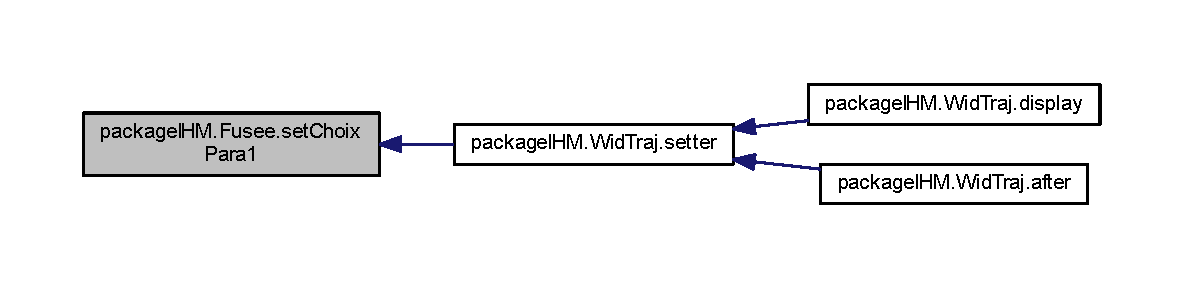
\includegraphics[width=350pt]{classpackage_i_h_m_1_1_fusee_ac5b5249cb12a38209d3a8b5f1770f7bd_icgraph}
\end{center}
\end{figure}
\mbox{\Hypertarget{classpackage_i_h_m_1_1_fusee_a4932fbd05f898de11de1ada5313f37cb}\label{classpackage_i_h_m_1_1_fusee_a4932fbd05f898de11de1ada5313f37cb}} 
\index{package\+I\+H\+M\+::\+Fusee@{package\+I\+H\+M\+::\+Fusee}!set\+Cn\+Ail@{set\+Cn\+Ail}}
\index{set\+Cn\+Ail@{set\+Cn\+Ail}!package\+I\+H\+M\+::\+Fusee@{package\+I\+H\+M\+::\+Fusee}}
\subsubsection{\texorpdfstring{set\+Cn\+Ail()}{setCnAil()}}
{\footnotesize\ttfamily void package\+I\+H\+M.\+Fusee.\+set\+Cn\+Ail (\begin{DoxyParamCaption}\item[{double}]{p\+Cn\+Ail }\end{DoxyParamCaption})}

Setters of the output data for the stability \mbox{\Hypertarget{classpackage_i_h_m_1_1_fusee_ac6e57258dd09efd5b0e299fa0812ade8}\label{classpackage_i_h_m_1_1_fusee_ac6e57258dd09efd5b0e299fa0812ade8}} 
\index{package\+I\+H\+M\+::\+Fusee@{package\+I\+H\+M\+::\+Fusee}!set\+Cn\+Can@{set\+Cn\+Can}}
\index{set\+Cn\+Can@{set\+Cn\+Can}!package\+I\+H\+M\+::\+Fusee@{package\+I\+H\+M\+::\+Fusee}}
\subsubsection{\texorpdfstring{set\+Cn\+Can()}{setCnCan()}}
{\footnotesize\ttfamily void package\+I\+H\+M.\+Fusee.\+set\+Cn\+Can (\begin{DoxyParamCaption}\item[{double}]{p\+Cn\+Can }\end{DoxyParamCaption})}

\mbox{\Hypertarget{classpackage_i_h_m_1_1_fusee_a4f15756423ff03fbeecf763c68384d72}\label{classpackage_i_h_m_1_1_fusee_a4f15756423ff03fbeecf763c68384d72}} 
\index{package\+I\+H\+M\+::\+Fusee@{package\+I\+H\+M\+::\+Fusee}!set\+Cn\+Masq@{set\+Cn\+Masq}}
\index{set\+Cn\+Masq@{set\+Cn\+Masq}!package\+I\+H\+M\+::\+Fusee@{package\+I\+H\+M\+::\+Fusee}}
\subsubsection{\texorpdfstring{set\+Cn\+Masq()}{setCnMasq()}}
{\footnotesize\ttfamily void package\+I\+H\+M.\+Fusee.\+set\+Cn\+Masq (\begin{DoxyParamCaption}\item[{double}]{p\+Cn\+Masq }\end{DoxyParamCaption})}

\mbox{\Hypertarget{classpackage_i_h_m_1_1_fusee_a98392042eda567ca22371fb406ce57d8}\label{classpackage_i_h_m_1_1_fusee_a98392042eda567ca22371fb406ce57d8}} 
\index{package\+I\+H\+M\+::\+Fusee@{package\+I\+H\+M\+::\+Fusee}!set\+Cx@{set\+Cx}}
\index{set\+Cx@{set\+Cx}!package\+I\+H\+M\+::\+Fusee@{package\+I\+H\+M\+::\+Fusee}}
\subsubsection{\texorpdfstring{set\+Cx()}{setCx()}}
{\footnotesize\ttfamily void package\+I\+H\+M.\+Fusee.\+set\+Cx (\begin{DoxyParamCaption}\item[{double}]{p\+Cx }\end{DoxyParamCaption})}

Here is the caller graph for this function\+:
\nopagebreak
\begin{figure}[H]
\begin{center}
\leavevmode
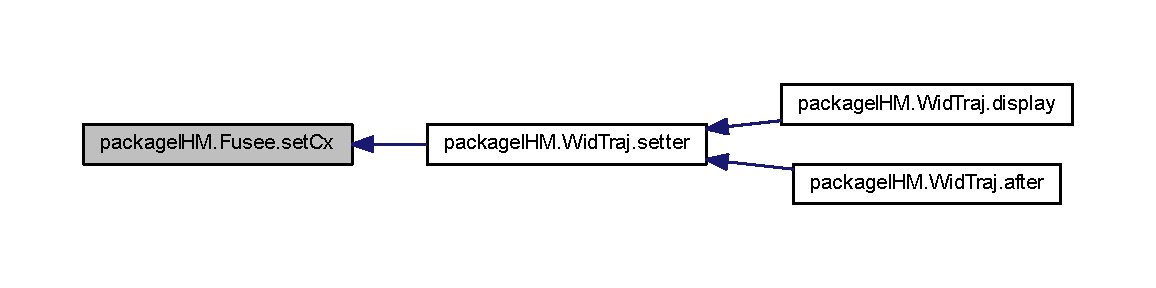
\includegraphics[width=350pt]{classpackage_i_h_m_1_1_fusee_a98392042eda567ca22371fb406ce57d8_icgraph}
\end{center}
\end{figure}
\mbox{\Hypertarget{classpackage_i_h_m_1_1_fusee_ae4e82628fb8e0d0959e5cc228dadde9d}\label{classpackage_i_h_m_1_1_fusee_ae4e82628fb8e0d0959e5cc228dadde9d}} 
\index{package\+I\+H\+M\+::\+Fusee@{package\+I\+H\+M\+::\+Fusee}!set\+Cx\+Para1@{set\+Cx\+Para1}}
\index{set\+Cx\+Para1@{set\+Cx\+Para1}!package\+I\+H\+M\+::\+Fusee@{package\+I\+H\+M\+::\+Fusee}}
\subsubsection{\texorpdfstring{set\+Cx\+Para1()}{setCxPara1()}}
{\footnotesize\ttfamily void package\+I\+H\+M.\+Fusee.\+set\+Cx\+Para1 (\begin{DoxyParamCaption}\item[{double}]{p\+Cx\+Para }\end{DoxyParamCaption})}

Here is the caller graph for this function\+:
\nopagebreak
\begin{figure}[H]
\begin{center}
\leavevmode
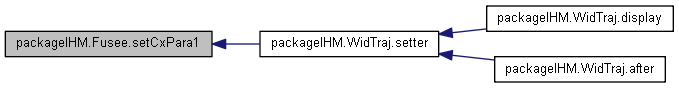
\includegraphics[width=350pt]{classpackage_i_h_m_1_1_fusee_ae4e82628fb8e0d0959e5cc228dadde9d_icgraph}
\end{center}
\end{figure}
\mbox{\Hypertarget{classpackage_i_h_m_1_1_fusee_a4d66174af42e3ac36e542391dc1f2955}\label{classpackage_i_h_m_1_1_fusee_a4d66174af42e3ac36e542391dc1f2955}} 
\index{package\+I\+H\+M\+::\+Fusee@{package\+I\+H\+M\+::\+Fusee}!set\+Cx\+Para2@{set\+Cx\+Para2}}
\index{set\+Cx\+Para2@{set\+Cx\+Para2}!package\+I\+H\+M\+::\+Fusee@{package\+I\+H\+M\+::\+Fusee}}
\subsubsection{\texorpdfstring{set\+Cx\+Para2()}{setCxPara2()}}
{\footnotesize\ttfamily void package\+I\+H\+M.\+Fusee.\+set\+Cx\+Para2 (\begin{DoxyParamCaption}\item[{double}]{p\+Cx\+Para }\end{DoxyParamCaption})}

Here is the caller graph for this function\+:
\nopagebreak
\begin{figure}[H]
\begin{center}
\leavevmode
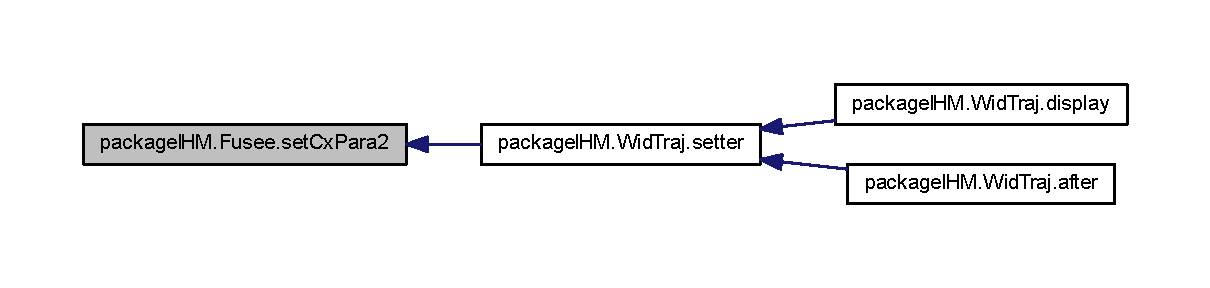
\includegraphics[width=350pt]{classpackage_i_h_m_1_1_fusee_a4d66174af42e3ac36e542391dc1f2955_icgraph}
\end{center}
\end{figure}
\mbox{\Hypertarget{classpackage_i_h_m_1_1_fusee_a87b1a260185adb8cc4da48d4e7c21ab2}\label{classpackage_i_h_m_1_1_fusee_a87b1a260185adb8cc4da48d4e7c21ab2}} 
\index{package\+I\+H\+M\+::\+Fusee@{package\+I\+H\+M\+::\+Fusee}!set\+D1A@{set\+D1A}}
\index{set\+D1A@{set\+D1A}!package\+I\+H\+M\+::\+Fusee@{package\+I\+H\+M\+::\+Fusee}}
\subsubsection{\texorpdfstring{set\+D1\+A()}{setD1A()}}
{\footnotesize\ttfamily void package\+I\+H\+M.\+Fusee.\+set\+D1A (\begin{DoxyParamCaption}\item[{double}]{p\+D1A }\end{DoxyParamCaption})}

Here is the caller graph for this function\+:
\nopagebreak
\begin{figure}[H]
\begin{center}
\leavevmode
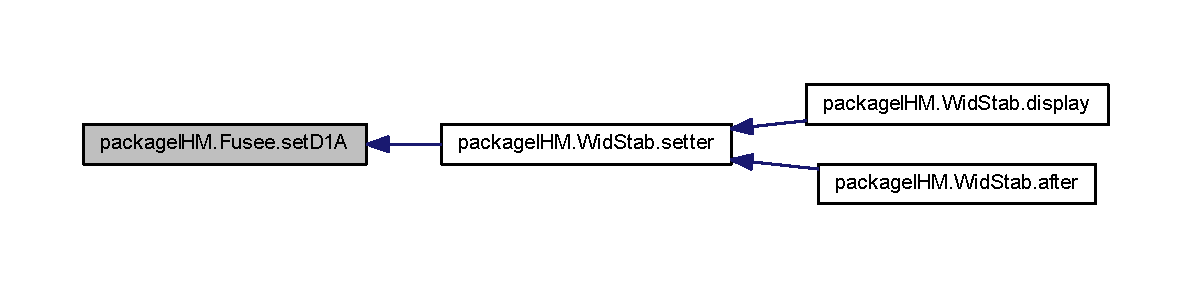
\includegraphics[width=350pt]{classpackage_i_h_m_1_1_fusee_a87b1a260185adb8cc4da48d4e7c21ab2_icgraph}
\end{center}
\end{figure}
\mbox{\Hypertarget{classpackage_i_h_m_1_1_fusee_aa323ec5a3bcfead8dbc544a134f7f5ff}\label{classpackage_i_h_m_1_1_fusee_aa323ec5a3bcfead8dbc544a134f7f5ff}} 
\index{package\+I\+H\+M\+::\+Fusee@{package\+I\+H\+M\+::\+Fusee}!set\+D1B@{set\+D1B}}
\index{set\+D1B@{set\+D1B}!package\+I\+H\+M\+::\+Fusee@{package\+I\+H\+M\+::\+Fusee}}
\subsubsection{\texorpdfstring{set\+D1\+B()}{setD1B()}}
{\footnotesize\ttfamily void package\+I\+H\+M.\+Fusee.\+set\+D1B (\begin{DoxyParamCaption}\item[{double}]{p\+D1B }\end{DoxyParamCaption})}

Here is the caller graph for this function\+:
\nopagebreak
\begin{figure}[H]
\begin{center}
\leavevmode
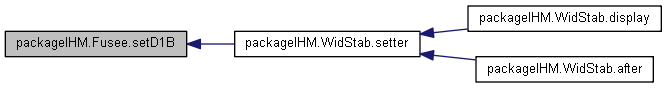
\includegraphics[width=350pt]{classpackage_i_h_m_1_1_fusee_aa323ec5a3bcfead8dbc544a134f7f5ff_icgraph}
\end{center}
\end{figure}
\mbox{\Hypertarget{classpackage_i_h_m_1_1_fusee_a9d8dbc7979eed99685708c96d0408e08}\label{classpackage_i_h_m_1_1_fusee_a9d8dbc7979eed99685708c96d0408e08}} 
\index{package\+I\+H\+M\+::\+Fusee@{package\+I\+H\+M\+::\+Fusee}!set\+D2A@{set\+D2A}}
\index{set\+D2A@{set\+D2A}!package\+I\+H\+M\+::\+Fusee@{package\+I\+H\+M\+::\+Fusee}}
\subsubsection{\texorpdfstring{set\+D2\+A()}{setD2A()}}
{\footnotesize\ttfamily void package\+I\+H\+M.\+Fusee.\+set\+D2A (\begin{DoxyParamCaption}\item[{double}]{p\+D2A }\end{DoxyParamCaption})}

Here is the caller graph for this function\+:
\nopagebreak
\begin{figure}[H]
\begin{center}
\leavevmode
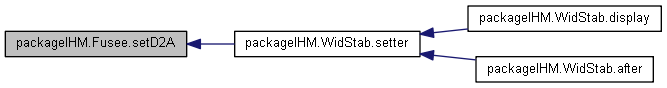
\includegraphics[width=350pt]{classpackage_i_h_m_1_1_fusee_a9d8dbc7979eed99685708c96d0408e08_icgraph}
\end{center}
\end{figure}
\mbox{\Hypertarget{classpackage_i_h_m_1_1_fusee_a6d2626133415ca045afa4145cd13f7ae}\label{classpackage_i_h_m_1_1_fusee_a6d2626133415ca045afa4145cd13f7ae}} 
\index{package\+I\+H\+M\+::\+Fusee@{package\+I\+H\+M\+::\+Fusee}!set\+D2B@{set\+D2B}}
\index{set\+D2B@{set\+D2B}!package\+I\+H\+M\+::\+Fusee@{package\+I\+H\+M\+::\+Fusee}}
\subsubsection{\texorpdfstring{set\+D2\+B()}{setD2B()}}
{\footnotesize\ttfamily void package\+I\+H\+M.\+Fusee.\+set\+D2B (\begin{DoxyParamCaption}\item[{double}]{p\+D2B }\end{DoxyParamCaption})}

Here is the caller graph for this function\+:
\nopagebreak
\begin{figure}[H]
\begin{center}
\leavevmode
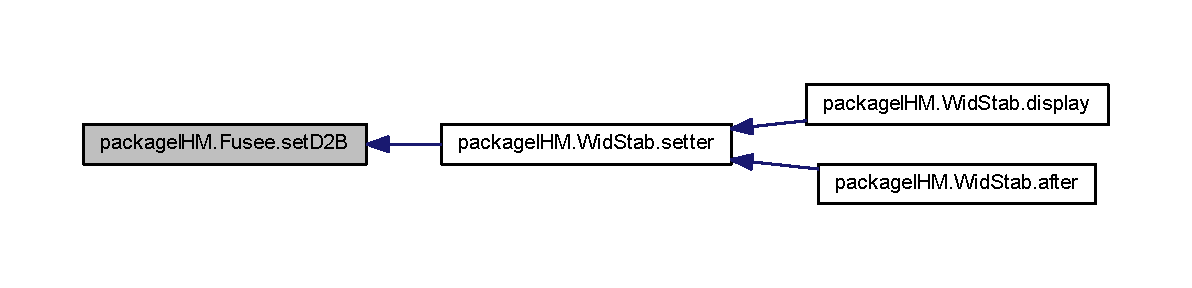
\includegraphics[width=350pt]{classpackage_i_h_m_1_1_fusee_a6d2626133415ca045afa4145cd13f7ae_icgraph}
\end{center}
\end{figure}
\mbox{\Hypertarget{classpackage_i_h_m_1_1_fusee_a4911cc2f18095344dbd65c7934fb3c21}\label{classpackage_i_h_m_1_1_fusee_a4911cc2f18095344dbd65c7934fb3c21}} 
\index{package\+I\+H\+M\+::\+Fusee@{package\+I\+H\+M\+::\+Fusee}!set\+D\+Ail@{set\+D\+Ail}}
\index{set\+D\+Ail@{set\+D\+Ail}!package\+I\+H\+M\+::\+Fusee@{package\+I\+H\+M\+::\+Fusee}}
\subsubsection{\texorpdfstring{set\+D\+Ail()}{setDAil()}}
{\footnotesize\ttfamily void package\+I\+H\+M.\+Fusee.\+set\+D\+Ail (\begin{DoxyParamCaption}\item[{double}]{p\+D\+Ail }\end{DoxyParamCaption})}

Here is the caller graph for this function\+:
\nopagebreak
\begin{figure}[H]
\begin{center}
\leavevmode
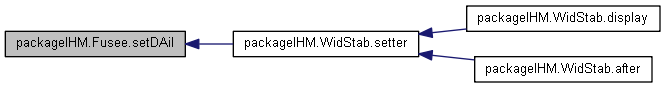
\includegraphics[width=350pt]{classpackage_i_h_m_1_1_fusee_a4911cc2f18095344dbd65c7934fb3c21_icgraph}
\end{center}
\end{figure}
\mbox{\Hypertarget{classpackage_i_h_m_1_1_fusee_a583bc99f76ddf6c953cf3b30f3107e6b}\label{classpackage_i_h_m_1_1_fusee_a583bc99f76ddf6c953cf3b30f3107e6b}} 
\index{package\+I\+H\+M\+::\+Fusee@{package\+I\+H\+M\+::\+Fusee}!set\+Date\+Acceleration\+Maximale@{set\+Date\+Acceleration\+Maximale}}
\index{set\+Date\+Acceleration\+Maximale@{set\+Date\+Acceleration\+Maximale}!package\+I\+H\+M\+::\+Fusee@{package\+I\+H\+M\+::\+Fusee}}
\subsubsection{\texorpdfstring{set\+Date\+Acceleration\+Maximale()}{setDateAccelerationMaximale()}}
{\footnotesize\ttfamily void package\+I\+H\+M.\+Fusee.\+set\+Date\+Acceleration\+Maximale (\begin{DoxyParamCaption}\item[{double}]{p\+Date\+Acceleration\+Maximale }\end{DoxyParamCaption})}

\mbox{\Hypertarget{classpackage_i_h_m_1_1_fusee_a68d93647d284438d1e8bc854e0dede28}\label{classpackage_i_h_m_1_1_fusee_a68d93647d284438d1e8bc854e0dede28}} 
\index{package\+I\+H\+M\+::\+Fusee@{package\+I\+H\+M\+::\+Fusee}!set\+Date\+Para1@{set\+Date\+Para1}}
\index{set\+Date\+Para1@{set\+Date\+Para1}!package\+I\+H\+M\+::\+Fusee@{package\+I\+H\+M\+::\+Fusee}}
\subsubsection{\texorpdfstring{set\+Date\+Para1()}{setDatePara1()}}
{\footnotesize\ttfamily void package\+I\+H\+M.\+Fusee.\+set\+Date\+Para1 (\begin{DoxyParamCaption}\item[{double}]{p\+Date\+Para }\end{DoxyParamCaption})}

Here is the caller graph for this function\+:
\nopagebreak
\begin{figure}[H]
\begin{center}
\leavevmode
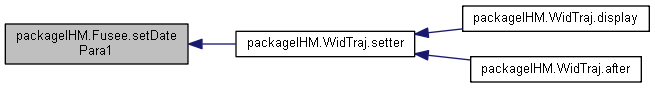
\includegraphics[width=350pt]{classpackage_i_h_m_1_1_fusee_a68d93647d284438d1e8bc854e0dede28_icgraph}
\end{center}
\end{figure}
\mbox{\Hypertarget{classpackage_i_h_m_1_1_fusee_a641ffd1bcd0dd6992bc522f831462eb8}\label{classpackage_i_h_m_1_1_fusee_a641ffd1bcd0dd6992bc522f831462eb8}} 
\index{package\+I\+H\+M\+::\+Fusee@{package\+I\+H\+M\+::\+Fusee}!set\+Date\+Para2@{set\+Date\+Para2}}
\index{set\+Date\+Para2@{set\+Date\+Para2}!package\+I\+H\+M\+::\+Fusee@{package\+I\+H\+M\+::\+Fusee}}
\subsubsection{\texorpdfstring{set\+Date\+Para2()}{setDatePara2()}}
{\footnotesize\ttfamily void package\+I\+H\+M.\+Fusee.\+set\+Date\+Para2 (\begin{DoxyParamCaption}\item[{double}]{p\+Date\+Para }\end{DoxyParamCaption})}

Here is the caller graph for this function\+:
\nopagebreak
\begin{figure}[H]
\begin{center}
\leavevmode
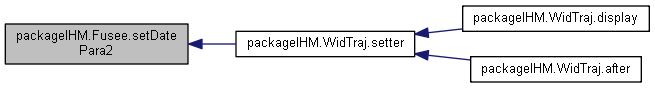
\includegraphics[width=350pt]{classpackage_i_h_m_1_1_fusee_a641ffd1bcd0dd6992bc522f831462eb8_icgraph}
\end{center}
\end{figure}
\mbox{\Hypertarget{classpackage_i_h_m_1_1_fusee_ab89fbbe48028772ed7edead723202629}\label{classpackage_i_h_m_1_1_fusee_ab89fbbe48028772ed7edead723202629}} 
\index{package\+I\+H\+M\+::\+Fusee@{package\+I\+H\+M\+::\+Fusee}!set\+Date\+Vitesse\+Maximale@{set\+Date\+Vitesse\+Maximale}}
\index{set\+Date\+Vitesse\+Maximale@{set\+Date\+Vitesse\+Maximale}!package\+I\+H\+M\+::\+Fusee@{package\+I\+H\+M\+::\+Fusee}}
\subsubsection{\texorpdfstring{set\+Date\+Vitesse\+Maximale()}{setDateVitesseMaximale()}}
{\footnotesize\ttfamily void package\+I\+H\+M.\+Fusee.\+set\+Date\+Vitesse\+Maximale (\begin{DoxyParamCaption}\item[{double}]{p\+Date\+Vitesse\+Maximale }\end{DoxyParamCaption})}

\mbox{\Hypertarget{classpackage_i_h_m_1_1_fusee_a882069f16bcea633d504abdf12adb784}\label{classpackage_i_h_m_1_1_fusee_a882069f16bcea633d504abdf12adb784}} 
\index{package\+I\+H\+M\+::\+Fusee@{package\+I\+H\+M\+::\+Fusee}!set\+D\+Can@{set\+D\+Can}}
\index{set\+D\+Can@{set\+D\+Can}!package\+I\+H\+M\+::\+Fusee@{package\+I\+H\+M\+::\+Fusee}}
\subsubsection{\texorpdfstring{set\+D\+Can()}{setDCan()}}
{\footnotesize\ttfamily void package\+I\+H\+M.\+Fusee.\+set\+D\+Can (\begin{DoxyParamCaption}\item[{double}]{p\+D\+Can }\end{DoxyParamCaption})}

Here is the caller graph for this function\+:
\nopagebreak
\begin{figure}[H]
\begin{center}
\leavevmode
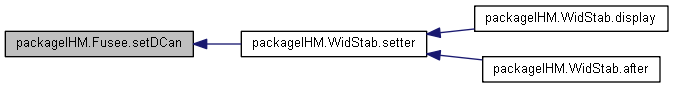
\includegraphics[width=350pt]{classpackage_i_h_m_1_1_fusee_a882069f16bcea633d504abdf12adb784_icgraph}
\end{center}
\end{figure}
\mbox{\Hypertarget{classpackage_i_h_m_1_1_fusee_a9ed5261755af5aaa36967db63e0bab65}\label{classpackage_i_h_m_1_1_fusee_a9ed5261755af5aaa36967db63e0bab65}} 
\index{package\+I\+H\+M\+::\+Fusee@{package\+I\+H\+M\+::\+Fusee}!set\+Dim1\+Para1@{set\+Dim1\+Para1}}
\index{set\+Dim1\+Para1@{set\+Dim1\+Para1}!package\+I\+H\+M\+::\+Fusee@{package\+I\+H\+M\+::\+Fusee}}
\subsubsection{\texorpdfstring{set\+Dim1\+Para1()}{setDim1Para1()}}
{\footnotesize\ttfamily void package\+I\+H\+M.\+Fusee.\+set\+Dim1\+Para1 (\begin{DoxyParamCaption}\item[{double}]{p\+Dim1\+Para1 }\end{DoxyParamCaption})}

Here is the caller graph for this function\+:
\nopagebreak
\begin{figure}[H]
\begin{center}
\leavevmode
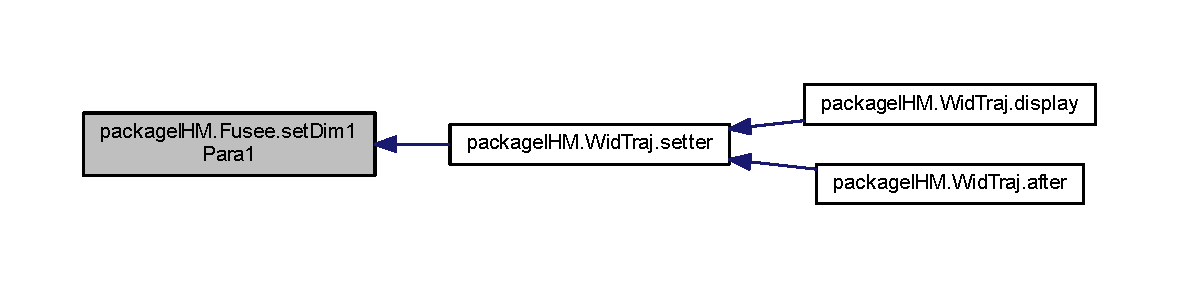
\includegraphics[width=350pt]{classpackage_i_h_m_1_1_fusee_a9ed5261755af5aaa36967db63e0bab65_icgraph}
\end{center}
\end{figure}
\mbox{\Hypertarget{classpackage_i_h_m_1_1_fusee_a1ff71d541b4033aad9fad18ffe946e00}\label{classpackage_i_h_m_1_1_fusee_a1ff71d541b4033aad9fad18ffe946e00}} 
\index{package\+I\+H\+M\+::\+Fusee@{package\+I\+H\+M\+::\+Fusee}!set\+Dim1\+Para2@{set\+Dim1\+Para2}}
\index{set\+Dim1\+Para2@{set\+Dim1\+Para2}!package\+I\+H\+M\+::\+Fusee@{package\+I\+H\+M\+::\+Fusee}}
\subsubsection{\texorpdfstring{set\+Dim1\+Para2()}{setDim1Para2()}}
{\footnotesize\ttfamily void package\+I\+H\+M.\+Fusee.\+set\+Dim1\+Para2 (\begin{DoxyParamCaption}\item[{double}]{p\+Dim1\+Para2 }\end{DoxyParamCaption})}

Here is the caller graph for this function\+:
\nopagebreak
\begin{figure}[H]
\begin{center}
\leavevmode
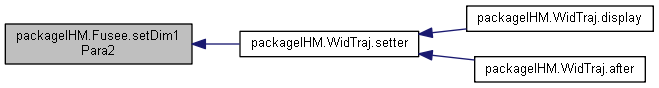
\includegraphics[width=350pt]{classpackage_i_h_m_1_1_fusee_a1ff71d541b4033aad9fad18ffe946e00_icgraph}
\end{center}
\end{figure}
\mbox{\Hypertarget{classpackage_i_h_m_1_1_fusee_ab98d4e52f22c9b6b2a42aa17b9712cb1}\label{classpackage_i_h_m_1_1_fusee_ab98d4e52f22c9b6b2a42aa17b9712cb1}} 
\index{package\+I\+H\+M\+::\+Fusee@{package\+I\+H\+M\+::\+Fusee}!set\+Dim2\+Para1@{set\+Dim2\+Para1}}
\index{set\+Dim2\+Para1@{set\+Dim2\+Para1}!package\+I\+H\+M\+::\+Fusee@{package\+I\+H\+M\+::\+Fusee}}
\subsubsection{\texorpdfstring{set\+Dim2\+Para1()}{setDim2Para1()}}
{\footnotesize\ttfamily void package\+I\+H\+M.\+Fusee.\+set\+Dim2\+Para1 (\begin{DoxyParamCaption}\item[{double}]{p\+Dim2\+Para1 }\end{DoxyParamCaption})}

Here is the caller graph for this function\+:
\nopagebreak
\begin{figure}[H]
\begin{center}
\leavevmode
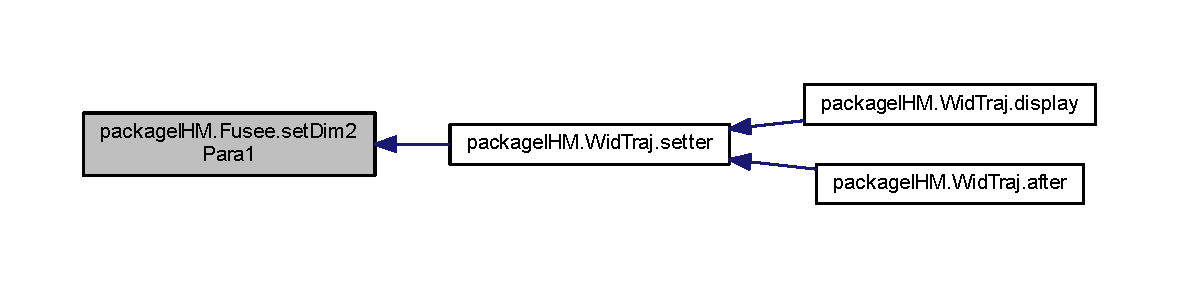
\includegraphics[width=350pt]{classpackage_i_h_m_1_1_fusee_ab98d4e52f22c9b6b2a42aa17b9712cb1_icgraph}
\end{center}
\end{figure}
\mbox{\Hypertarget{classpackage_i_h_m_1_1_fusee_ad7d5fb59177dba7096636b20899a0217}\label{classpackage_i_h_m_1_1_fusee_ad7d5fb59177dba7096636b20899a0217}} 
\index{package\+I\+H\+M\+::\+Fusee@{package\+I\+H\+M\+::\+Fusee}!set\+Dim2\+Para2@{set\+Dim2\+Para2}}
\index{set\+Dim2\+Para2@{set\+Dim2\+Para2}!package\+I\+H\+M\+::\+Fusee@{package\+I\+H\+M\+::\+Fusee}}
\subsubsection{\texorpdfstring{set\+Dim2\+Para2()}{setDim2Para2()}}
{\footnotesize\ttfamily void package\+I\+H\+M.\+Fusee.\+set\+Dim2\+Para2 (\begin{DoxyParamCaption}\item[{double}]{p\+Dim2\+Para2 }\end{DoxyParamCaption})}

Here is the caller graph for this function\+:
\nopagebreak
\begin{figure}[H]
\begin{center}
\leavevmode
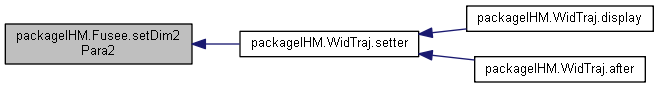
\includegraphics[width=350pt]{classpackage_i_h_m_1_1_fusee_ad7d5fb59177dba7096636b20899a0217_icgraph}
\end{center}
\end{figure}
\mbox{\Hypertarget{classpackage_i_h_m_1_1_fusee_a7bd7ff5fdfb52d094a47ab4dc6868e85}\label{classpackage_i_h_m_1_1_fusee_a7bd7ff5fdfb52d094a47ab4dc6868e85}} 
\index{package\+I\+H\+M\+::\+Fusee@{package\+I\+H\+M\+::\+Fusee}!set\+D\+Ogive@{set\+D\+Ogive}}
\index{set\+D\+Ogive@{set\+D\+Ogive}!package\+I\+H\+M\+::\+Fusee@{package\+I\+H\+M\+::\+Fusee}}
\subsubsection{\texorpdfstring{set\+D\+Ogive()}{setDOgive()}}
{\footnotesize\ttfamily void package\+I\+H\+M.\+Fusee.\+set\+D\+Ogive (\begin{DoxyParamCaption}\item[{double}]{p\+D\+Og }\end{DoxyParamCaption})}

Here is the caller graph for this function\+:
\nopagebreak
\begin{figure}[H]
\begin{center}
\leavevmode
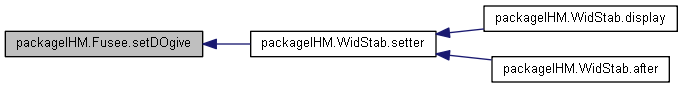
\includegraphics[width=350pt]{classpackage_i_h_m_1_1_fusee_a7bd7ff5fdfb52d094a47ab4dc6868e85_icgraph}
\end{center}
\end{figure}
\mbox{\Hypertarget{classpackage_i_h_m_1_1_fusee_a767306a1f843f3152f9fe8875c630db5}\label{classpackage_i_h_m_1_1_fusee_a767306a1f843f3152f9fe8875c630db5}} 
\index{package\+I\+H\+M\+::\+Fusee@{package\+I\+H\+M\+::\+Fusee}!set\+D\+Ref@{set\+D\+Ref}}
\index{set\+D\+Ref@{set\+D\+Ref}!package\+I\+H\+M\+::\+Fusee@{package\+I\+H\+M\+::\+Fusee}}
\subsubsection{\texorpdfstring{set\+D\+Ref()}{setDRef()}}
{\footnotesize\ttfamily void package\+I\+H\+M.\+Fusee.\+set\+D\+Ref (\begin{DoxyParamCaption}\item[{double}]{p\+D\+Ref }\end{DoxyParamCaption})}

Here is the caller graph for this function\+:
\nopagebreak
\begin{figure}[H]
\begin{center}
\leavevmode
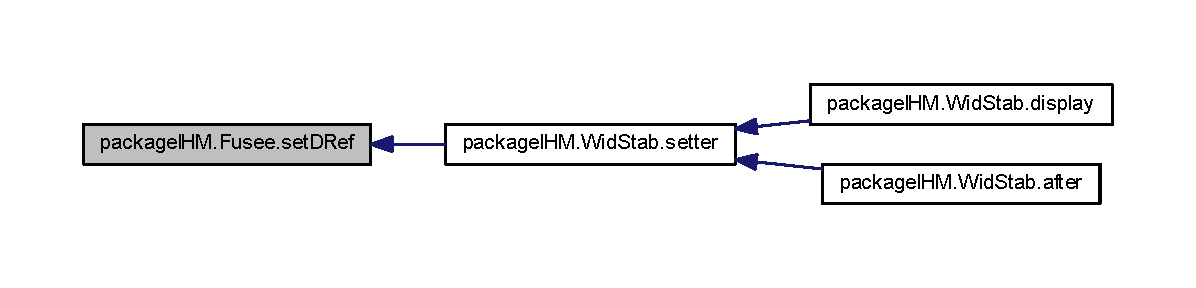
\includegraphics[width=350pt]{classpackage_i_h_m_1_1_fusee_a767306a1f843f3152f9fe8875c630db5_icgraph}
\end{center}
\end{figure}
\mbox{\Hypertarget{classpackage_i_h_m_1_1_fusee_ad93195b0678feb43125f3f2c537f4f69}\label{classpackage_i_h_m_1_1_fusee_ad93195b0678feb43125f3f2c537f4f69}} 
\index{package\+I\+H\+M\+::\+Fusee@{package\+I\+H\+M\+::\+Fusee}!set\+Duree\+Vol@{set\+Duree\+Vol}}
\index{set\+Duree\+Vol@{set\+Duree\+Vol}!package\+I\+H\+M\+::\+Fusee@{package\+I\+H\+M\+::\+Fusee}}
\subsubsection{\texorpdfstring{set\+Duree\+Vol()}{setDureeVol()}}
{\footnotesize\ttfamily void package\+I\+H\+M.\+Fusee.\+set\+Duree\+Vol (\begin{DoxyParamCaption}\item[{double}]{p\+Duree\+Vol }\end{DoxyParamCaption})}

\mbox{\Hypertarget{classpackage_i_h_m_1_1_fusee_a8fb6a108f0382c97bfa361f9455f20f6}\label{classpackage_i_h_m_1_1_fusee_a8fb6a108f0382c97bfa361f9455f20f6}} 
\index{package\+I\+H\+M\+::\+Fusee@{package\+I\+H\+M\+::\+Fusee}!set\+D\+Vol@{set\+D\+Vol}}
\index{set\+D\+Vol@{set\+D\+Vol}!package\+I\+H\+M\+::\+Fusee@{package\+I\+H\+M\+::\+Fusee}}
\subsubsection{\texorpdfstring{set\+D\+Vol()}{setDVol()}}
{\footnotesize\ttfamily void package\+I\+H\+M.\+Fusee.\+set\+D\+Vol (\begin{DoxyParamCaption}\item[{double}]{p\+D\+Vol }\end{DoxyParamCaption})}

\mbox{\Hypertarget{classpackage_i_h_m_1_1_fusee_acde45292d46c140cf574cd10f692d2bf}\label{classpackage_i_h_m_1_1_fusee_acde45292d46c140cf574cd10f692d2bf}} 
\index{package\+I\+H\+M\+::\+Fusee@{package\+I\+H\+M\+::\+Fusee}!set\+Emplanture\+Ail@{set\+Emplanture\+Ail}}
\index{set\+Emplanture\+Ail@{set\+Emplanture\+Ail}!package\+I\+H\+M\+::\+Fusee@{package\+I\+H\+M\+::\+Fusee}}
\subsubsection{\texorpdfstring{set\+Emplanture\+Ail()}{setEmplantureAil()}}
{\footnotesize\ttfamily void package\+I\+H\+M.\+Fusee.\+set\+Emplanture\+Ail (\begin{DoxyParamCaption}\item[{double}]{p\+M\+Ail }\end{DoxyParamCaption})}

Here is the caller graph for this function\+:
\nopagebreak
\begin{figure}[H]
\begin{center}
\leavevmode
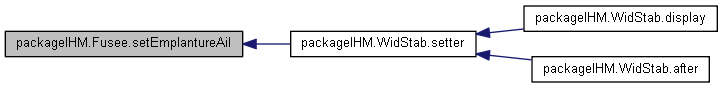
\includegraphics[width=350pt]{classpackage_i_h_m_1_1_fusee_acde45292d46c140cf574cd10f692d2bf_icgraph}
\end{center}
\end{figure}
\mbox{\Hypertarget{classpackage_i_h_m_1_1_fusee_a60ce8f710340e05a0e04e8592629f207}\label{classpackage_i_h_m_1_1_fusee_a60ce8f710340e05a0e04e8592629f207}} 
\index{package\+I\+H\+M\+::\+Fusee@{package\+I\+H\+M\+::\+Fusee}!set\+Emplanture\+Can@{set\+Emplanture\+Can}}
\index{set\+Emplanture\+Can@{set\+Emplanture\+Can}!package\+I\+H\+M\+::\+Fusee@{package\+I\+H\+M\+::\+Fusee}}
\subsubsection{\texorpdfstring{set\+Emplanture\+Can()}{setEmplantureCan()}}
{\footnotesize\ttfamily void package\+I\+H\+M.\+Fusee.\+set\+Emplanture\+Can (\begin{DoxyParamCaption}\item[{double}]{p\+M\+Can }\end{DoxyParamCaption})}

Here is the caller graph for this function\+:
\nopagebreak
\begin{figure}[H]
\begin{center}
\leavevmode
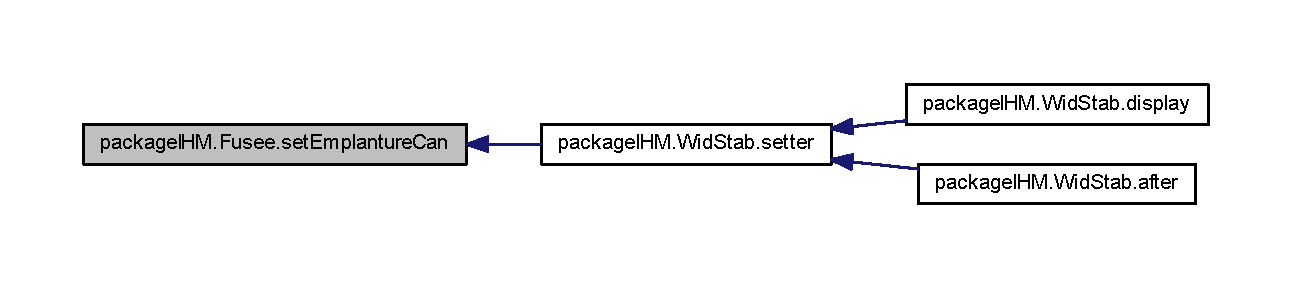
\includegraphics[width=350pt]{classpackage_i_h_m_1_1_fusee_a60ce8f710340e05a0e04e8592629f207_icgraph}
\end{center}
\end{figure}
\mbox{\Hypertarget{classpackage_i_h_m_1_1_fusee_a095ad2f563f226e729a17bf173caae0c}\label{classpackage_i_h_m_1_1_fusee_a095ad2f563f226e729a17bf173caae0c}} 
\index{package\+I\+H\+M\+::\+Fusee@{package\+I\+H\+M\+::\+Fusee}!set\+Envergure\+Ail@{set\+Envergure\+Ail}}
\index{set\+Envergure\+Ail@{set\+Envergure\+Ail}!package\+I\+H\+M\+::\+Fusee@{package\+I\+H\+M\+::\+Fusee}}
\subsubsection{\texorpdfstring{set\+Envergure\+Ail()}{setEnvergureAil()}}
{\footnotesize\ttfamily void package\+I\+H\+M.\+Fusee.\+set\+Envergure\+Ail (\begin{DoxyParamCaption}\item[{double}]{p\+E\+Ail }\end{DoxyParamCaption})}

Here is the caller graph for this function\+:
\nopagebreak
\begin{figure}[H]
\begin{center}
\leavevmode
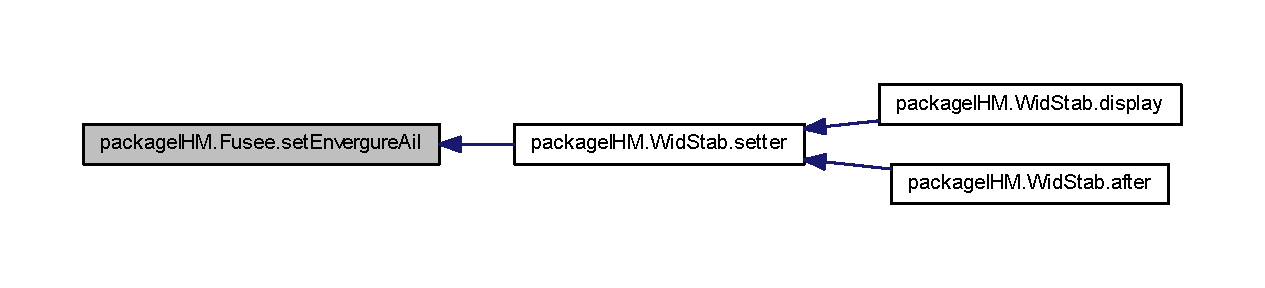
\includegraphics[width=350pt]{classpackage_i_h_m_1_1_fusee_a095ad2f563f226e729a17bf173caae0c_icgraph}
\end{center}
\end{figure}
\mbox{\Hypertarget{classpackage_i_h_m_1_1_fusee_a5bf57b456ec7544fa37785c1b90cbdb8}\label{classpackage_i_h_m_1_1_fusee_a5bf57b456ec7544fa37785c1b90cbdb8}} 
\index{package\+I\+H\+M\+::\+Fusee@{package\+I\+H\+M\+::\+Fusee}!set\+Envergure\+Can@{set\+Envergure\+Can}}
\index{set\+Envergure\+Can@{set\+Envergure\+Can}!package\+I\+H\+M\+::\+Fusee@{package\+I\+H\+M\+::\+Fusee}}
\subsubsection{\texorpdfstring{set\+Envergure\+Can()}{setEnvergureCan()}}
{\footnotesize\ttfamily void package\+I\+H\+M.\+Fusee.\+set\+Envergure\+Can (\begin{DoxyParamCaption}\item[{double}]{p\+E\+Can }\end{DoxyParamCaption})}

Here is the caller graph for this function\+:
\nopagebreak
\begin{figure}[H]
\begin{center}
\leavevmode
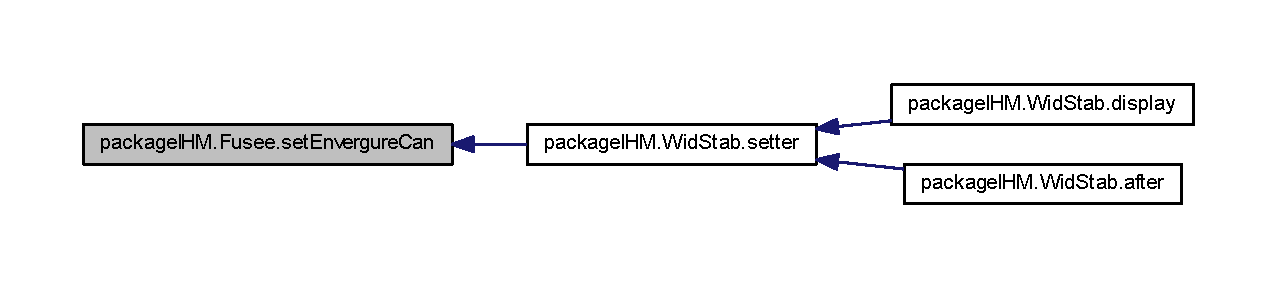
\includegraphics[width=350pt]{classpackage_i_h_m_1_1_fusee_a5bf57b456ec7544fa37785c1b90cbdb8_icgraph}
\end{center}
\end{figure}
\mbox{\Hypertarget{classpackage_i_h_m_1_1_fusee_a438fc23f5f692504651ea9befd9d6080}\label{classpackage_i_h_m_1_1_fusee_a438fc23f5f692504651ea9befd9d6080}} 
\index{package\+I\+H\+M\+::\+Fusee@{package\+I\+H\+M\+::\+Fusee}!set\+Envergure\+Masq@{set\+Envergure\+Masq}}
\index{set\+Envergure\+Masq@{set\+Envergure\+Masq}!package\+I\+H\+M\+::\+Fusee@{package\+I\+H\+M\+::\+Fusee}}
\subsubsection{\texorpdfstring{set\+Envergure\+Masq()}{setEnvergureMasq()}}
{\footnotesize\ttfamily void package\+I\+H\+M.\+Fusee.\+set\+Envergure\+Masq (\begin{DoxyParamCaption}\item[{double}]{p\+Envergure\+Masq }\end{DoxyParamCaption})}

\mbox{\Hypertarget{classpackage_i_h_m_1_1_fusee_a9f238ddf7075ac84479926b56ff34a93}\label{classpackage_i_h_m_1_1_fusee_a9f238ddf7075ac84479926b56ff34a93}} 
\index{package\+I\+H\+M\+::\+Fusee@{package\+I\+H\+M\+::\+Fusee}!set\+Ep\+Ail@{set\+Ep\+Ail}}
\index{set\+Ep\+Ail@{set\+Ep\+Ail}!package\+I\+H\+M\+::\+Fusee@{package\+I\+H\+M\+::\+Fusee}}
\subsubsection{\texorpdfstring{set\+Ep\+Ail()}{setEpAil()}}
{\footnotesize\ttfamily void package\+I\+H\+M.\+Fusee.\+set\+Ep\+Ail (\begin{DoxyParamCaption}\item[{double}]{p\+Ep\+Ail }\end{DoxyParamCaption})}

Setters of the intput data for the trajectory Here is the caller graph for this function\+:
\nopagebreak
\begin{figure}[H]
\begin{center}
\leavevmode
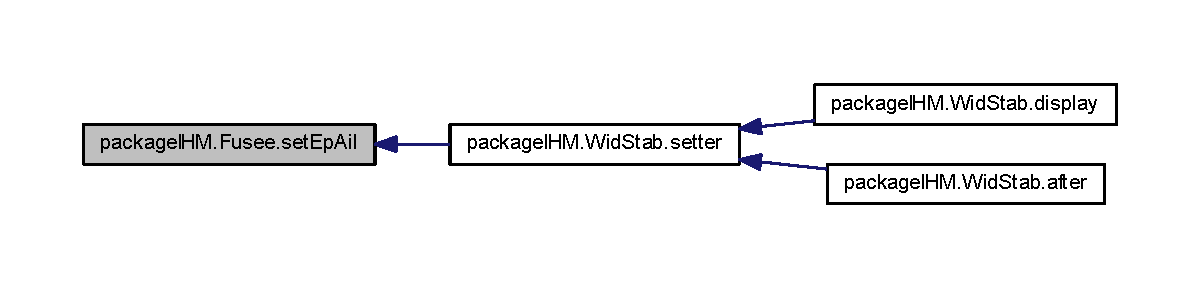
\includegraphics[width=350pt]{classpackage_i_h_m_1_1_fusee_a9f238ddf7075ac84479926b56ff34a93_icgraph}
\end{center}
\end{figure}
\mbox{\Hypertarget{classpackage_i_h_m_1_1_fusee_a150cfda175a96df36732867427ebb9a7}\label{classpackage_i_h_m_1_1_fusee_a150cfda175a96df36732867427ebb9a7}} 
\index{package\+I\+H\+M\+::\+Fusee@{package\+I\+H\+M\+::\+Fusee}!set\+Ep\+Can@{set\+Ep\+Can}}
\index{set\+Ep\+Can@{set\+Ep\+Can}!package\+I\+H\+M\+::\+Fusee@{package\+I\+H\+M\+::\+Fusee}}
\subsubsection{\texorpdfstring{set\+Ep\+Can()}{setEpCan()}}
{\footnotesize\ttfamily void package\+I\+H\+M.\+Fusee.\+set\+Ep\+Can (\begin{DoxyParamCaption}\item[{double}]{p\+Ep\+Can }\end{DoxyParamCaption})}

Here is the caller graph for this function\+:
\nopagebreak
\begin{figure}[H]
\begin{center}
\leavevmode
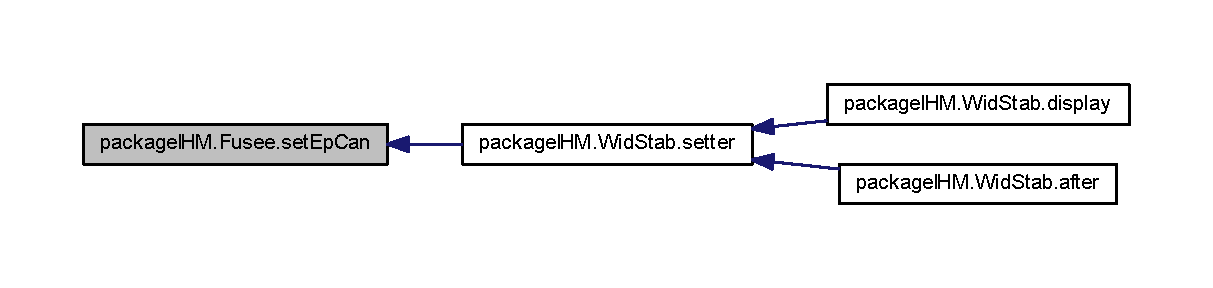
\includegraphics[width=350pt]{classpackage_i_h_m_1_1_fusee_a150cfda175a96df36732867427ebb9a7_icgraph}
\end{center}
\end{figure}
\mbox{\Hypertarget{classpackage_i_h_m_1_1_fusee_adee696c2be77ba2bb4c50942a529b8aa}\label{classpackage_i_h_m_1_1_fusee_adee696c2be77ba2bb4c50942a529b8aa}} 
\index{package\+I\+H\+M\+::\+Fusee@{package\+I\+H\+M\+::\+Fusee}!set\+Etat\+Moteur@{set\+Etat\+Moteur}}
\index{set\+Etat\+Moteur@{set\+Etat\+Moteur}!package\+I\+H\+M\+::\+Fusee@{package\+I\+H\+M\+::\+Fusee}}
\subsubsection{\texorpdfstring{set\+Etat\+Moteur()}{setEtatMoteur()}}
{\footnotesize\ttfamily void package\+I\+H\+M.\+Fusee.\+set\+Etat\+Moteur (\begin{DoxyParamCaption}\item[{int}]{p\+Etat\+Moteur }\end{DoxyParamCaption})}

Here is the caller graph for this function\+:
\nopagebreak
\begin{figure}[H]
\begin{center}
\leavevmode
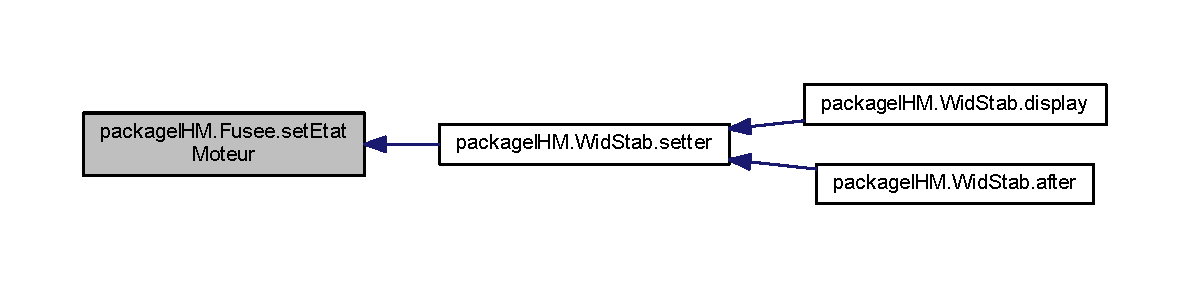
\includegraphics[width=350pt]{classpackage_i_h_m_1_1_fusee_adee696c2be77ba2bb4c50942a529b8aa_icgraph}
\end{center}
\end{figure}
\mbox{\Hypertarget{classpackage_i_h_m_1_1_fusee_a76788e837a543a6939f3c962251e7301}\label{classpackage_i_h_m_1_1_fusee_a76788e837a543a6939f3c962251e7301}} 
\index{package\+I\+H\+M\+::\+Fusee@{package\+I\+H\+M\+::\+Fusee}!setfleche\+Ail@{setfleche\+Ail}}
\index{setfleche\+Ail@{setfleche\+Ail}!package\+I\+H\+M\+::\+Fusee@{package\+I\+H\+M\+::\+Fusee}}
\subsubsection{\texorpdfstring{setfleche\+Ail()}{setflecheAil()}}
{\footnotesize\ttfamily void package\+I\+H\+M.\+Fusee.\+setfleche\+Ail (\begin{DoxyParamCaption}\item[{double}]{p\+P\+Ail }\end{DoxyParamCaption})}

Here is the caller graph for this function\+:
\nopagebreak
\begin{figure}[H]
\begin{center}
\leavevmode
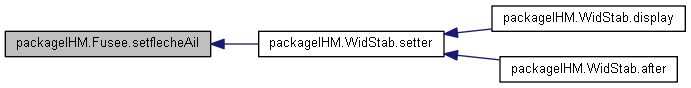
\includegraphics[width=350pt]{classpackage_i_h_m_1_1_fusee_a76788e837a543a6939f3c962251e7301_icgraph}
\end{center}
\end{figure}
\mbox{\Hypertarget{classpackage_i_h_m_1_1_fusee_a03644d01af83beee8b3ec160b8122792}\label{classpackage_i_h_m_1_1_fusee_a03644d01af83beee8b3ec160b8122792}} 
\index{package\+I\+H\+M\+::\+Fusee@{package\+I\+H\+M\+::\+Fusee}!set\+Fleche\+Can@{set\+Fleche\+Can}}
\index{set\+Fleche\+Can@{set\+Fleche\+Can}!package\+I\+H\+M\+::\+Fusee@{package\+I\+H\+M\+::\+Fusee}}
\subsubsection{\texorpdfstring{set\+Fleche\+Can()}{setFlecheCan()}}
{\footnotesize\ttfamily void package\+I\+H\+M.\+Fusee.\+set\+Fleche\+Can (\begin{DoxyParamCaption}\item[{double}]{p\+P\+Can }\end{DoxyParamCaption})}

Here is the caller graph for this function\+:
\nopagebreak
\begin{figure}[H]
\begin{center}
\leavevmode
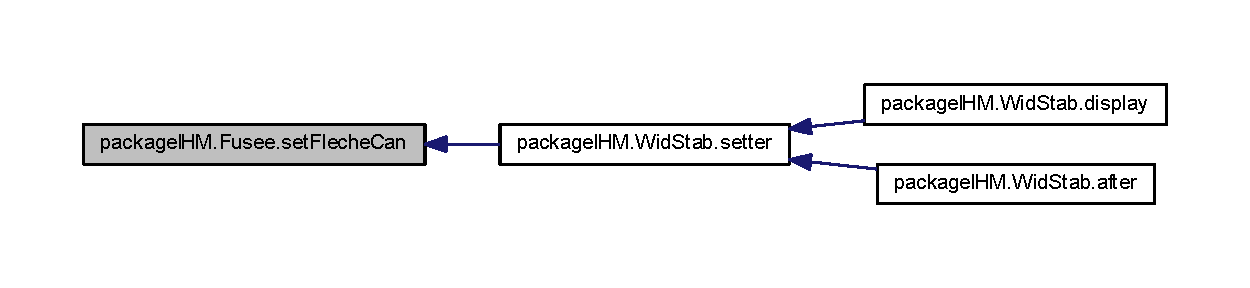
\includegraphics[width=350pt]{classpackage_i_h_m_1_1_fusee_a03644d01af83beee8b3ec160b8122792_icgraph}
\end{center}
\end{figure}
\mbox{\Hypertarget{classpackage_i_h_m_1_1_fusee_ad4e7aed5da90790b85a55f449dc369bf}\label{classpackage_i_h_m_1_1_fusee_ad4e7aed5da90790b85a55f449dc369bf}} 
\index{package\+I\+H\+M\+::\+Fusee@{package\+I\+H\+M\+::\+Fusee}!set\+Inst\+Culmination@{set\+Inst\+Culmination}}
\index{set\+Inst\+Culmination@{set\+Inst\+Culmination}!package\+I\+H\+M\+::\+Fusee@{package\+I\+H\+M\+::\+Fusee}}
\subsubsection{\texorpdfstring{set\+Inst\+Culmination()}{setInstCulmination()}}
{\footnotesize\ttfamily void package\+I\+H\+M.\+Fusee.\+set\+Inst\+Culmination (\begin{DoxyParamCaption}\item[{double}]{p\+Inst\+Culmination }\end{DoxyParamCaption})}

\mbox{\Hypertarget{classpackage_i_h_m_1_1_fusee_ab1443ccbef6ceaf2d88b454422d1459f}\label{classpackage_i_h_m_1_1_fusee_ab1443ccbef6ceaf2d88b454422d1459f}} 
\index{package\+I\+H\+M\+::\+Fusee@{package\+I\+H\+M\+::\+Fusee}!set\+LA@{set\+LA}}
\index{set\+LA@{set\+LA}!package\+I\+H\+M\+::\+Fusee@{package\+I\+H\+M\+::\+Fusee}}
\subsubsection{\texorpdfstring{set\+L\+A()}{setLA()}}
{\footnotesize\ttfamily void package\+I\+H\+M.\+Fusee.\+set\+LA (\begin{DoxyParamCaption}\item[{double}]{p\+LA }\end{DoxyParamCaption})}

Here is the caller graph for this function\+:
\nopagebreak
\begin{figure}[H]
\begin{center}
\leavevmode
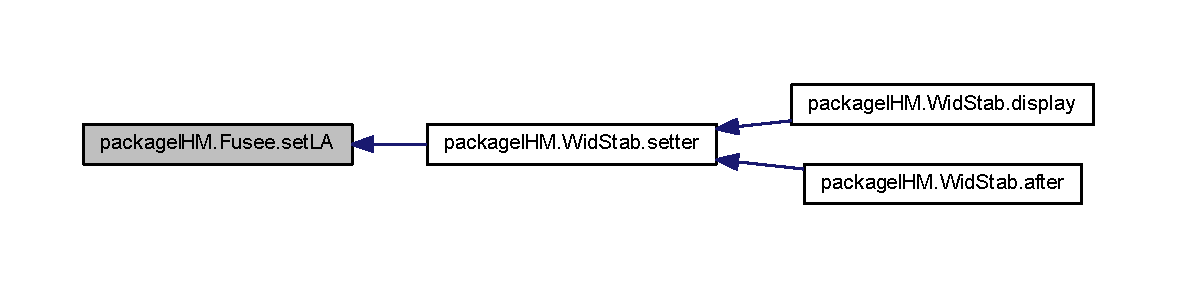
\includegraphics[width=350pt]{classpackage_i_h_m_1_1_fusee_ab1443ccbef6ceaf2d88b454422d1459f_icgraph}
\end{center}
\end{figure}
\mbox{\Hypertarget{classpackage_i_h_m_1_1_fusee_ad118c4ee9278838ed86a9013f27f5209}\label{classpackage_i_h_m_1_1_fusee_ad118c4ee9278838ed86a9013f27f5209}} 
\index{package\+I\+H\+M\+::\+Fusee@{package\+I\+H\+M\+::\+Fusee}!set\+LB@{set\+LB}}
\index{set\+LB@{set\+LB}!package\+I\+H\+M\+::\+Fusee@{package\+I\+H\+M\+::\+Fusee}}
\subsubsection{\texorpdfstring{set\+L\+B()}{setLB()}}
{\footnotesize\ttfamily void package\+I\+H\+M.\+Fusee.\+set\+LB (\begin{DoxyParamCaption}\item[{double}]{p\+LB }\end{DoxyParamCaption})}

Here is the caller graph for this function\+:
\nopagebreak
\begin{figure}[H]
\begin{center}
\leavevmode
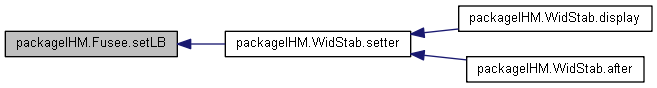
\includegraphics[width=350pt]{classpackage_i_h_m_1_1_fusee_ad118c4ee9278838ed86a9013f27f5209_icgraph}
\end{center}
\end{figure}
\mbox{\Hypertarget{classpackage_i_h_m_1_1_fusee_a3c255fb77f49e09df344b04881a91af0}\label{classpackage_i_h_m_1_1_fusee_a3c255fb77f49e09df344b04881a91af0}} 
\index{package\+I\+H\+M\+::\+Fusee@{package\+I\+H\+M\+::\+Fusee}!set\+Long@{set\+Long}}
\index{set\+Long@{set\+Long}!package\+I\+H\+M\+::\+Fusee@{package\+I\+H\+M\+::\+Fusee}}
\subsubsection{\texorpdfstring{set\+Long()}{setLong()}}
{\footnotesize\ttfamily void package\+I\+H\+M.\+Fusee.\+set\+Long (\begin{DoxyParamCaption}\item[{double}]{p\+Long }\end{DoxyParamCaption})}

Here is the caller graph for this function\+:
\nopagebreak
\begin{figure}[H]
\begin{center}
\leavevmode
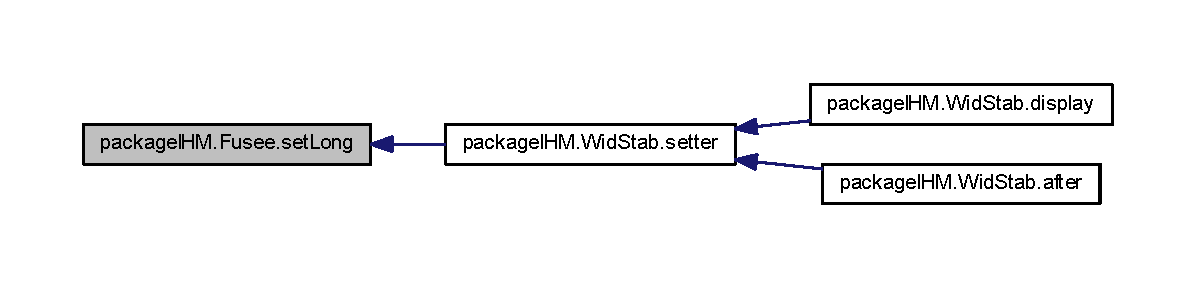
\includegraphics[width=350pt]{classpackage_i_h_m_1_1_fusee_a3c255fb77f49e09df344b04881a91af0_icgraph}
\end{center}
\end{figure}
\mbox{\Hypertarget{classpackage_i_h_m_1_1_fusee_a99fd69516f079c4726a5a69d2cd26264}\label{classpackage_i_h_m_1_1_fusee_a99fd69516f079c4726a5a69d2cd26264}} 
\index{package\+I\+H\+M\+::\+Fusee@{package\+I\+H\+M\+::\+Fusee}!set\+Long\+Ogive@{set\+Long\+Ogive}}
\index{set\+Long\+Ogive@{set\+Long\+Ogive}!package\+I\+H\+M\+::\+Fusee@{package\+I\+H\+M\+::\+Fusee}}
\subsubsection{\texorpdfstring{set\+Long\+Ogive()}{setLongOgive()}}
{\footnotesize\ttfamily void package\+I\+H\+M.\+Fusee.\+set\+Long\+Ogive (\begin{DoxyParamCaption}\item[{double}]{p\+Long\+Og }\end{DoxyParamCaption})}

Here is the caller graph for this function\+:
\nopagebreak
\begin{figure}[H]
\begin{center}
\leavevmode
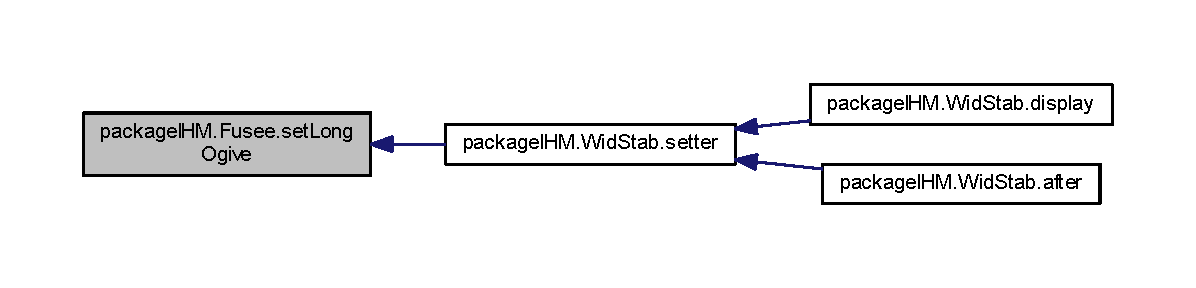
\includegraphics[width=350pt]{classpackage_i_h_m_1_1_fusee_a99fd69516f079c4726a5a69d2cd26264_icgraph}
\end{center}
\end{figure}
\mbox{\Hypertarget{classpackage_i_h_m_1_1_fusee_a8d5576c59efc33927e23e6ab0497a8b7}\label{classpackage_i_h_m_1_1_fusee_a8d5576c59efc33927e23e6ab0497a8b7}} 
\index{package\+I\+H\+M\+::\+Fusee@{package\+I\+H\+M\+::\+Fusee}!set\+L\+Rampe@{set\+L\+Rampe}}
\index{set\+L\+Rampe@{set\+L\+Rampe}!package\+I\+H\+M\+::\+Fusee@{package\+I\+H\+M\+::\+Fusee}}
\subsubsection{\texorpdfstring{set\+L\+Rampe()}{setLRampe()}}
{\footnotesize\ttfamily void package\+I\+H\+M.\+Fusee.\+set\+L\+Rampe (\begin{DoxyParamCaption}\item[{double}]{p\+L\+Rampe }\end{DoxyParamCaption})}

Here is the caller graph for this function\+:
\nopagebreak
\begin{figure}[H]
\begin{center}
\leavevmode
\includegraphics[width=350pt]{classpackage_i_h_m_1_1_fusee_a8d5576c59efc33927e23e6ab0497a8b7_icgraph}
\end{center}
\end{figure}
\mbox{\Hypertarget{classpackage_i_h_m_1_1_fusee_a09712bc7d39d33d86a7f0e792afe8e81}\label{classpackage_i_h_m_1_1_fusee_a09712bc7d39d33d86a7f0e792afe8e81}} 
\index{package\+I\+H\+M\+::\+Fusee@{package\+I\+H\+M\+::\+Fusee}!set\+Mach\+Max@{set\+Mach\+Max}}
\index{set\+Mach\+Max@{set\+Mach\+Max}!package\+I\+H\+M\+::\+Fusee@{package\+I\+H\+M\+::\+Fusee}}
\subsubsection{\texorpdfstring{set\+Mach\+Max()}{setMachMax()}}
{\footnotesize\ttfamily void package\+I\+H\+M.\+Fusee.\+set\+Mach\+Max (\begin{DoxyParamCaption}\item[{double}]{p\+Mach\+Max }\end{DoxyParamCaption})}

\mbox{\Hypertarget{classpackage_i_h_m_1_1_fusee_af9b328549d361cc5e110d9f4728baa54}\label{classpackage_i_h_m_1_1_fusee_af9b328549d361cc5e110d9f4728baa54}} 
\index{package\+I\+H\+M\+::\+Fusee@{package\+I\+H\+M\+::\+Fusee}!set\+Masse\+Moteur\+Plein@{set\+Masse\+Moteur\+Plein}}
\index{set\+Masse\+Moteur\+Plein@{set\+Masse\+Moteur\+Plein}!package\+I\+H\+M\+::\+Fusee@{package\+I\+H\+M\+::\+Fusee}}
\subsubsection{\texorpdfstring{set\+Masse\+Moteur\+Plein()}{setMasseMoteurPlein()}}
{\footnotesize\ttfamily void package\+I\+H\+M.\+Fusee.\+set\+Masse\+Moteur\+Plein (\begin{DoxyParamCaption}\item[{double}]{p\+Masse }\end{DoxyParamCaption})}

Here is the caller graph for this function\+:
\nopagebreak
\begin{figure}[H]
\begin{center}
\leavevmode
\includegraphics[width=350pt]{classpackage_i_h_m_1_1_fusee_af9b328549d361cc5e110d9f4728baa54_icgraph}
\end{center}
\end{figure}
\mbox{\Hypertarget{classpackage_i_h_m_1_1_fusee_a8125616eb55dd45142ee7da5c6a59139}\label{classpackage_i_h_m_1_1_fusee_a8125616eb55dd45142ee7da5c6a59139}} 
\index{package\+I\+H\+M\+::\+Fusee@{package\+I\+H\+M\+::\+Fusee}!set\+Masse\+Para@{set\+Masse\+Para}}
\index{set\+Masse\+Para@{set\+Masse\+Para}!package\+I\+H\+M\+::\+Fusee@{package\+I\+H\+M\+::\+Fusee}}
\subsubsection{\texorpdfstring{set\+Masse\+Para()}{setMassePara()}}
{\footnotesize\ttfamily void package\+I\+H\+M.\+Fusee.\+set\+Masse\+Para (\begin{DoxyParamCaption}\item[{double}]{p\+Masse\+Para }\end{DoxyParamCaption})}

\mbox{\Hypertarget{classpackage_i_h_m_1_1_fusee_afc93358b04fb82fbd0bd77b9d4cb176c}\label{classpackage_i_h_m_1_1_fusee_afc93358b04fb82fbd0bd77b9d4cb176c}} 
\index{package\+I\+H\+M\+::\+Fusee@{package\+I\+H\+M\+::\+Fusee}!set\+Masse\+Sans\+Moteur@{set\+Masse\+Sans\+Moteur}}
\index{set\+Masse\+Sans\+Moteur@{set\+Masse\+Sans\+Moteur}!package\+I\+H\+M\+::\+Fusee@{package\+I\+H\+M\+::\+Fusee}}
\subsubsection{\texorpdfstring{set\+Masse\+Sans\+Moteur()}{setMasseSansMoteur()}}
{\footnotesize\ttfamily void package\+I\+H\+M.\+Fusee.\+set\+Masse\+Sans\+Moteur (\begin{DoxyParamCaption}\item[{double}]{p\+Masse }\end{DoxyParamCaption})}

Here is the caller graph for this function\+:
\nopagebreak
\begin{figure}[H]
\begin{center}
\leavevmode
\includegraphics[width=350pt]{classpackage_i_h_m_1_1_fusee_afc93358b04fb82fbd0bd77b9d4cb176c_icgraph}
\end{center}
\end{figure}
\mbox{\Hypertarget{classpackage_i_h_m_1_1_fusee_accd7cf5c7efadea4cce60020c27df3fa}\label{classpackage_i_h_m_1_1_fusee_accd7cf5c7efadea4cce60020c27df3fa}} 
\index{package\+I\+H\+M\+::\+Fusee@{package\+I\+H\+M\+::\+Fusee}!set\+M\+Max@{set\+M\+Max}}
\index{set\+M\+Max@{set\+M\+Max}!package\+I\+H\+M\+::\+Fusee@{package\+I\+H\+M\+::\+Fusee}}
\subsubsection{\texorpdfstring{set\+M\+Max()}{setMMax()}}
{\footnotesize\ttfamily void package\+I\+H\+M.\+Fusee.\+set\+M\+Max (\begin{DoxyParamCaption}\item[{double}]{p\+M\+Max }\end{DoxyParamCaption})}

\mbox{\Hypertarget{classpackage_i_h_m_1_1_fusee_a73408b99915edfdee5af928b1c3d52d8}\label{classpackage_i_h_m_1_1_fusee_a73408b99915edfdee5af928b1c3d52d8}} 
\index{package\+I\+H\+M\+::\+Fusee@{package\+I\+H\+M\+::\+Fusee}!set\+M\+S\+Min@{set\+M\+S\+Min}}
\index{set\+M\+S\+Min@{set\+M\+S\+Min}!package\+I\+H\+M\+::\+Fusee@{package\+I\+H\+M\+::\+Fusee}}
\subsubsection{\texorpdfstring{set\+M\+S\+Min()}{setMSMin()}}
{\footnotesize\ttfamily void package\+I\+H\+M.\+Fusee.\+set\+M\+S\+Min (\begin{DoxyParamCaption}\item[{double}]{p\+M\+S\+Min }\end{DoxyParamCaption})}

\mbox{\Hypertarget{classpackage_i_h_m_1_1_fusee_a44f18e21695e9398158f114dc2e9e574}\label{classpackage_i_h_m_1_1_fusee_a44f18e21695e9398158f114dc2e9e574}} 
\index{package\+I\+H\+M\+::\+Fusee@{package\+I\+H\+M\+::\+Fusee}!set\+Nombre\+Ail@{set\+Nombre\+Ail}}
\index{set\+Nombre\+Ail@{set\+Nombre\+Ail}!package\+I\+H\+M\+::\+Fusee@{package\+I\+H\+M\+::\+Fusee}}
\subsubsection{\texorpdfstring{set\+Nombre\+Ail()}{setNombreAil()}}
{\footnotesize\ttfamily void package\+I\+H\+M.\+Fusee.\+set\+Nombre\+Ail (\begin{DoxyParamCaption}\item[{int}]{pD }\end{DoxyParamCaption})}

Here is the caller graph for this function\+:
\nopagebreak
\begin{figure}[H]
\begin{center}
\leavevmode
\includegraphics[width=350pt]{classpackage_i_h_m_1_1_fusee_a44f18e21695e9398158f114dc2e9e574_icgraph}
\end{center}
\end{figure}
\mbox{\Hypertarget{classpackage_i_h_m_1_1_fusee_ae44d0433f10fc3f57a94890e0d30b178}\label{classpackage_i_h_m_1_1_fusee_ae44d0433f10fc3f57a94890e0d30b178}} 
\index{package\+I\+H\+M\+::\+Fusee@{package\+I\+H\+M\+::\+Fusee}!set\+Nombre\+Can@{set\+Nombre\+Can}}
\index{set\+Nombre\+Can@{set\+Nombre\+Can}!package\+I\+H\+M\+::\+Fusee@{package\+I\+H\+M\+::\+Fusee}}
\subsubsection{\texorpdfstring{set\+Nombre\+Can()}{setNombreCan()}}
{\footnotesize\ttfamily void package\+I\+H\+M.\+Fusee.\+set\+Nombre\+Can (\begin{DoxyParamCaption}\item[{int}]{p\+D\+Can }\end{DoxyParamCaption})}

Here is the caller graph for this function\+:
\nopagebreak
\begin{figure}[H]
\begin{center}
\leavevmode
\includegraphics[width=350pt]{classpackage_i_h_m_1_1_fusee_ae44d0433f10fc3f57a94890e0d30b178_icgraph}
\end{center}
\end{figure}
\mbox{\Hypertarget{classpackage_i_h_m_1_1_fusee_a9954e75785e80ddb121a7e50218baaea}\label{classpackage_i_h_m_1_1_fusee_a9954e75785e80ddb121a7e50218baaea}} 
\index{package\+I\+H\+M\+::\+Fusee@{package\+I\+H\+M\+::\+Fusee}!set\+Nombre\+Jeux\+Ail@{set\+Nombre\+Jeux\+Ail}}
\index{set\+Nombre\+Jeux\+Ail@{set\+Nombre\+Jeux\+Ail}!package\+I\+H\+M\+::\+Fusee@{package\+I\+H\+M\+::\+Fusee}}
\subsubsection{\texorpdfstring{set\+Nombre\+Jeux\+Ail()}{setNombreJeuxAil()}}
{\footnotesize\ttfamily void package\+I\+H\+M.\+Fusee.\+set\+Nombre\+Jeux\+Ail (\begin{DoxyParamCaption}\item[{int}]{p\+Nb\+Jeux\+Ail }\end{DoxyParamCaption})}

Here is the caller graph for this function\+:
\nopagebreak
\begin{figure}[H]
\begin{center}
\leavevmode
\includegraphics[width=350pt]{classpackage_i_h_m_1_1_fusee_a9954e75785e80ddb121a7e50218baaea_icgraph}
\end{center}
\end{figure}
\mbox{\Hypertarget{classpackage_i_h_m_1_1_fusee_a5b3de7fcfa2b63969b5c51cb0172d517}\label{classpackage_i_h_m_1_1_fusee_a5b3de7fcfa2b63969b5c51cb0172d517}} 
\index{package\+I\+H\+M\+::\+Fusee@{package\+I\+H\+M\+::\+Fusee}!set\+Nombre\+Parachutes@{set\+Nombre\+Parachutes}}
\index{set\+Nombre\+Parachutes@{set\+Nombre\+Parachutes}!package\+I\+H\+M\+::\+Fusee@{package\+I\+H\+M\+::\+Fusee}}
\subsubsection{\texorpdfstring{set\+Nombre\+Parachutes()}{setNombreParachutes()}}
{\footnotesize\ttfamily void package\+I\+H\+M.\+Fusee.\+set\+Nombre\+Parachutes (\begin{DoxyParamCaption}\item[{int}]{p\+Nombre\+Parachutes }\end{DoxyParamCaption})}

Here is the caller graph for this function\+:
\nopagebreak
\begin{figure}[H]
\begin{center}
\leavevmode
\includegraphics[width=350pt]{classpackage_i_h_m_1_1_fusee_a5b3de7fcfa2b63969b5c51cb0172d517_icgraph}
\end{center}
\end{figure}
\mbox{\Hypertarget{classpackage_i_h_m_1_1_fusee_a3bdf31ee73dc1106750420449e448651}\label{classpackage_i_h_m_1_1_fusee_a3bdf31ee73dc1106750420449e448651}} 
\index{package\+I\+H\+M\+::\+Fusee@{package\+I\+H\+M\+::\+Fusee}!set\+Nombre\+Transitions@{set\+Nombre\+Transitions}}
\index{set\+Nombre\+Transitions@{set\+Nombre\+Transitions}!package\+I\+H\+M\+::\+Fusee@{package\+I\+H\+M\+::\+Fusee}}
\subsubsection{\texorpdfstring{set\+Nombre\+Transitions()}{setNombreTransitions()}}
{\footnotesize\ttfamily void package\+I\+H\+M.\+Fusee.\+set\+Nombre\+Transitions (\begin{DoxyParamCaption}\item[{int}]{p\+Nb\+Transitions }\end{DoxyParamCaption})}

Here is the caller graph for this function\+:
\nopagebreak
\begin{figure}[H]
\begin{center}
\leavevmode
\includegraphics[width=350pt]{classpackage_i_h_m_1_1_fusee_a3bdf31ee73dc1106750420449e448651_icgraph}
\end{center}
\end{figure}
\mbox{\Hypertarget{classpackage_i_h_m_1_1_fusee_aeee79c2de1bf0fe1f65afbe112437cb9}\label{classpackage_i_h_m_1_1_fusee_aeee79c2de1bf0fe1f65afbe112437cb9}} 
\index{package\+I\+H\+M\+::\+Fusee@{package\+I\+H\+M\+::\+Fusee}!set\+Nom\+Moteur@{set\+Nom\+Moteur}}
\index{set\+Nom\+Moteur@{set\+Nom\+Moteur}!package\+I\+H\+M\+::\+Fusee@{package\+I\+H\+M\+::\+Fusee}}
\subsubsection{\texorpdfstring{set\+Nom\+Moteur()}{setNomMoteur()}}
{\footnotesize\ttfamily void package\+I\+H\+M.\+Fusee.\+set\+Nom\+Moteur (\begin{DoxyParamCaption}\item[{String}]{p\+Moteur }\end{DoxyParamCaption})}

Here is the caller graph for this function\+:
\nopagebreak
\begin{figure}[H]
\begin{center}
\leavevmode
\includegraphics[width=350pt]{classpackage_i_h_m_1_1_fusee_aeee79c2de1bf0fe1f65afbe112437cb9_icgraph}
\end{center}
\end{figure}
\mbox{\Hypertarget{classpackage_i_h_m_1_1_fusee_ab9d6b405e661e93354c9601f4f5af296}\label{classpackage_i_h_m_1_1_fusee_ab9d6b405e661e93354c9601f4f5af296}} 
\index{package\+I\+H\+M\+::\+Fusee@{package\+I\+H\+M\+::\+Fusee}!set\+Port\+Balist@{set\+Port\+Balist}}
\index{set\+Port\+Balist@{set\+Port\+Balist}!package\+I\+H\+M\+::\+Fusee@{package\+I\+H\+M\+::\+Fusee}}
\subsubsection{\texorpdfstring{set\+Port\+Balist()}{setPortBalist()}}
{\footnotesize\ttfamily void package\+I\+H\+M.\+Fusee.\+set\+Port\+Balist (\begin{DoxyParamCaption}\item[{double}]{p\+Port\+Balist }\end{DoxyParamCaption})}

\mbox{\Hypertarget{classpackage_i_h_m_1_1_fusee_a83206f19aecc7c04f17b7cba17572473}\label{classpackage_i_h_m_1_1_fusee_a83206f19aecc7c04f17b7cba17572473}} 
\index{package\+I\+H\+M\+::\+Fusee@{package\+I\+H\+M\+::\+Fusee}!set\+Portee\+Balistique@{set\+Portee\+Balistique}}
\index{set\+Portee\+Balistique@{set\+Portee\+Balistique}!package\+I\+H\+M\+::\+Fusee@{package\+I\+H\+M\+::\+Fusee}}
\subsubsection{\texorpdfstring{set\+Portee\+Balistique()}{setPorteeBalistique()}}
{\footnotesize\ttfamily void package\+I\+H\+M.\+Fusee.\+set\+Portee\+Balistique (\begin{DoxyParamCaption}\item[{double}]{p\+Portee\+Balistique }\end{DoxyParamCaption})}

\mbox{\Hypertarget{classpackage_i_h_m_1_1_fusee_ab2de5bad20509bed7a38a0b2ff90c7e1}\label{classpackage_i_h_m_1_1_fusee_ab2de5bad20509bed7a38a0b2ff90c7e1}} 
\index{package\+I\+H\+M\+::\+Fusee@{package\+I\+H\+M\+::\+Fusee}!set\+Saumon\+Ail@{set\+Saumon\+Ail}}
\index{set\+Saumon\+Ail@{set\+Saumon\+Ail}!package\+I\+H\+M\+::\+Fusee@{package\+I\+H\+M\+::\+Fusee}}
\subsubsection{\texorpdfstring{set\+Saumon\+Ail()}{setSaumonAil()}}
{\footnotesize\ttfamily void package\+I\+H\+M.\+Fusee.\+set\+Saumon\+Ail (\begin{DoxyParamCaption}\item[{double}]{p\+N\+Ail }\end{DoxyParamCaption})}

Here is the caller graph for this function\+:
\nopagebreak
\begin{figure}[H]
\begin{center}
\leavevmode
\includegraphics[width=350pt]{classpackage_i_h_m_1_1_fusee_ab2de5bad20509bed7a38a0b2ff90c7e1_icgraph}
\end{center}
\end{figure}
\mbox{\Hypertarget{classpackage_i_h_m_1_1_fusee_a64ea7614bc794756aef51d5d7dc87c33}\label{classpackage_i_h_m_1_1_fusee_a64ea7614bc794756aef51d5d7dc87c33}} 
\index{package\+I\+H\+M\+::\+Fusee@{package\+I\+H\+M\+::\+Fusee}!set\+Saumon\+Can@{set\+Saumon\+Can}}
\index{set\+Saumon\+Can@{set\+Saumon\+Can}!package\+I\+H\+M\+::\+Fusee@{package\+I\+H\+M\+::\+Fusee}}
\subsubsection{\texorpdfstring{set\+Saumon\+Can()}{setSaumonCan()}}
{\footnotesize\ttfamily void package\+I\+H\+M.\+Fusee.\+set\+Saumon\+Can (\begin{DoxyParamCaption}\item[{double}]{p\+N\+Can }\end{DoxyParamCaption})}

Here is the caller graph for this function\+:
\nopagebreak
\begin{figure}[H]
\begin{center}
\leavevmode
\includegraphics[width=350pt]{classpackage_i_h_m_1_1_fusee_a64ea7614bc794756aef51d5d7dc87c33_icgraph}
\end{center}
\end{figure}
\mbox{\Hypertarget{classpackage_i_h_m_1_1_fusee_a425cd829802d0b1ae1c23a75adf65158}\label{classpackage_i_h_m_1_1_fusee_a425cd829802d0b1ae1c23a75adf65158}} 
\index{package\+I\+H\+M\+::\+Fusee@{package\+I\+H\+M\+::\+Fusee}!set\+S\+Ref\+Trainee@{set\+S\+Ref\+Trainee}}
\index{set\+S\+Ref\+Trainee@{set\+S\+Ref\+Trainee}!package\+I\+H\+M\+::\+Fusee@{package\+I\+H\+M\+::\+Fusee}}
\subsubsection{\texorpdfstring{set\+S\+Ref\+Trainee()}{setSRefTrainee()}}
{\footnotesize\ttfamily void package\+I\+H\+M.\+Fusee.\+set\+S\+Ref\+Trainee (\begin{DoxyParamCaption}\item[{double}]{p\+S\+Ref }\end{DoxyParamCaption})}

\mbox{\Hypertarget{classpackage_i_h_m_1_1_fusee_a2bffb174db259afdf0bd8c9bd8bcd54c}\label{classpackage_i_h_m_1_1_fusee_a2bffb174db259afdf0bd8c9bd8bcd54c}} 
\index{package\+I\+H\+M\+::\+Fusee@{package\+I\+H\+M\+::\+Fusee}!set\+Surface\+Para1@{set\+Surface\+Para1}}
\index{set\+Surface\+Para1@{set\+Surface\+Para1}!package\+I\+H\+M\+::\+Fusee@{package\+I\+H\+M\+::\+Fusee}}
\subsubsection{\texorpdfstring{set\+Surface\+Para1()}{setSurfacePara1()}}
{\footnotesize\ttfamily void package\+I\+H\+M.\+Fusee.\+set\+Surface\+Para1 (\begin{DoxyParamCaption}\item[{double}]{p\+Surf\+Para1 }\end{DoxyParamCaption})}

public void set\+Surface\+Para(double p\+Surf\+Para) \{ this.\+surface\+Para\+Totale = p\+Surf\+Para; \} Here is the caller graph for this function\+:
\nopagebreak
\begin{figure}[H]
\begin{center}
\leavevmode
\includegraphics[width=350pt]{classpackage_i_h_m_1_1_fusee_a2bffb174db259afdf0bd8c9bd8bcd54c_icgraph}
\end{center}
\end{figure}
\mbox{\Hypertarget{classpackage_i_h_m_1_1_fusee_adaedd5ad40ee9db9b1d1953761b35580}\label{classpackage_i_h_m_1_1_fusee_adaedd5ad40ee9db9b1d1953761b35580}} 
\index{package\+I\+H\+M\+::\+Fusee@{package\+I\+H\+M\+::\+Fusee}!set\+Surface\+Para2@{set\+Surface\+Para2}}
\index{set\+Surface\+Para2@{set\+Surface\+Para2}!package\+I\+H\+M\+::\+Fusee@{package\+I\+H\+M\+::\+Fusee}}
\subsubsection{\texorpdfstring{set\+Surface\+Para2()}{setSurfacePara2()}}
{\footnotesize\ttfamily void package\+I\+H\+M.\+Fusee.\+set\+Surface\+Para2 (\begin{DoxyParamCaption}\item[{double}]{p\+Surf\+Para1 }\end{DoxyParamCaption})}

Here is the caller graph for this function\+:
\nopagebreak
\begin{figure}[H]
\begin{center}
\leavevmode
\includegraphics[width=350pt]{classpackage_i_h_m_1_1_fusee_adaedd5ad40ee9db9b1d1953761b35580_icgraph}
\end{center}
\end{figure}
\mbox{\Hypertarget{classpackage_i_h_m_1_1_fusee_a221471781c00bad553488bd17a896957}\label{classpackage_i_h_m_1_1_fusee_a221471781c00bad553488bd17a896957}} 
\index{package\+I\+H\+M\+::\+Fusee@{package\+I\+H\+M\+::\+Fusee}!set\+T\+Balist@{set\+T\+Balist}}
\index{set\+T\+Balist@{set\+T\+Balist}!package\+I\+H\+M\+::\+Fusee@{package\+I\+H\+M\+::\+Fusee}}
\subsubsection{\texorpdfstring{set\+T\+Balist()}{setTBalist()}}
{\footnotesize\ttfamily void package\+I\+H\+M.\+Fusee.\+set\+T\+Balist (\begin{DoxyParamCaption}\item[{double}]{p\+T\+Balist }\end{DoxyParamCaption})}

\mbox{\Hypertarget{classpackage_i_h_m_1_1_fusee_a99ac0271424ea4a3d34c2e3c3d843164}\label{classpackage_i_h_m_1_1_fusee_a99ac0271424ea4a3d34c2e3c3d843164}} 
\index{package\+I\+H\+M\+::\+Fusee@{package\+I\+H\+M\+::\+Fusee}!set\+Temps\+Culmination@{set\+Temps\+Culmination}}
\index{set\+Temps\+Culmination@{set\+Temps\+Culmination}!package\+I\+H\+M\+::\+Fusee@{package\+I\+H\+M\+::\+Fusee}}
\subsubsection{\texorpdfstring{set\+Temps\+Culmination()}{setTempsCulmination()}}
{\footnotesize\ttfamily void package\+I\+H\+M.\+Fusee.\+set\+Temps\+Culmination (\begin{DoxyParamCaption}\item[{double}]{p\+Temps\+Culmination }\end{DoxyParamCaption})}

\mbox{\Hypertarget{classpackage_i_h_m_1_1_fusee_a726c750ee19c46330a25cc8b2249e3e5}\label{classpackage_i_h_m_1_1_fusee_a726c750ee19c46330a25cc8b2249e3e5}} 
\index{package\+I\+H\+M\+::\+Fusee@{package\+I\+H\+M\+::\+Fusee}!set\+Temps\+Fin\+Prop@{set\+Temps\+Fin\+Prop}}
\index{set\+Temps\+Fin\+Prop@{set\+Temps\+Fin\+Prop}!package\+I\+H\+M\+::\+Fusee@{package\+I\+H\+M\+::\+Fusee}}
\subsubsection{\texorpdfstring{set\+Temps\+Fin\+Prop()}{setTempsFinProp()}}
{\footnotesize\ttfamily void package\+I\+H\+M.\+Fusee.\+set\+Temps\+Fin\+Prop (\begin{DoxyParamCaption}\item[{double}]{p\+Temps\+Fin\+Prop }\end{DoxyParamCaption})}

\mbox{\Hypertarget{classpackage_i_h_m_1_1_fusee_a565696aea0d2c2d6de0c1e97df4a0595}\label{classpackage_i_h_m_1_1_fusee_a565696aea0d2c2d6de0c1e97df4a0595}} 
\index{package\+I\+H\+M\+::\+Fusee@{package\+I\+H\+M\+::\+Fusee}!set\+Type\+Fusee@{set\+Type\+Fusee}}
\index{set\+Type\+Fusee@{set\+Type\+Fusee}!package\+I\+H\+M\+::\+Fusee@{package\+I\+H\+M\+::\+Fusee}}
\subsubsection{\texorpdfstring{set\+Type\+Fusee()}{setTypeFusee()}}
{\footnotesize\ttfamily void package\+I\+H\+M.\+Fusee.\+set\+Type\+Fusee (\begin{DoxyParamCaption}\item[{int}]{p\+Type\+Fusee }\end{DoxyParamCaption})}



dur�e totale du vol (en s) 

Setters of the entry data for the stability considerations Here is the caller graph for this function\+:
\nopagebreak
\begin{figure}[H]
\begin{center}
\leavevmode
\includegraphics[width=350pt]{classpackage_i_h_m_1_1_fusee_a565696aea0d2c2d6de0c1e97df4a0595_icgraph}
\end{center}
\end{figure}
\mbox{\Hypertarget{classpackage_i_h_m_1_1_fusee_a8b46ca6157234a62c23ca2d23b5ed5f4}\label{classpackage_i_h_m_1_1_fusee_a8b46ca6157234a62c23ca2d23b5ed5f4}} 
\index{package\+I\+H\+M\+::\+Fusee@{package\+I\+H\+M\+::\+Fusee}!set\+Type\+Ogive@{set\+Type\+Ogive}}
\index{set\+Type\+Ogive@{set\+Type\+Ogive}!package\+I\+H\+M\+::\+Fusee@{package\+I\+H\+M\+::\+Fusee}}
\subsubsection{\texorpdfstring{set\+Type\+Ogive()}{setTypeOgive()}}
{\footnotesize\ttfamily void package\+I\+H\+M.\+Fusee.\+set\+Type\+Ogive (\begin{DoxyParamCaption}\item[{int}]{p\+Type\+Ogive }\end{DoxyParamCaption})}

Here is the caller graph for this function\+:
\nopagebreak
\begin{figure}[H]
\begin{center}
\leavevmode
\includegraphics[width=350pt]{classpackage_i_h_m_1_1_fusee_a8b46ca6157234a62c23ca2d23b5ed5f4_icgraph}
\end{center}
\end{figure}
\mbox{\Hypertarget{classpackage_i_h_m_1_1_fusee_a5769426d43b950c1aab90616ae88901b}\label{classpackage_i_h_m_1_1_fusee_a5769426d43b950c1aab90616ae88901b}} 
\index{package\+I\+H\+M\+::\+Fusee@{package\+I\+H\+M\+::\+Fusee}!set\+Vit\+Culmination@{set\+Vit\+Culmination}}
\index{set\+Vit\+Culmination@{set\+Vit\+Culmination}!package\+I\+H\+M\+::\+Fusee@{package\+I\+H\+M\+::\+Fusee}}
\subsubsection{\texorpdfstring{set\+Vit\+Culmination()}{setVitCulmination()}}
{\footnotesize\ttfamily void package\+I\+H\+M.\+Fusee.\+set\+Vit\+Culmination (\begin{DoxyParamCaption}\item[{double}]{p\+Vit\+Culmination }\end{DoxyParamCaption})}

\mbox{\Hypertarget{classpackage_i_h_m_1_1_fusee_a7101d60099df5944d5967c1a9ae0a4fd}\label{classpackage_i_h_m_1_1_fusee_a7101d60099df5944d5967c1a9ae0a4fd}} 
\index{package\+I\+H\+M\+::\+Fusee@{package\+I\+H\+M\+::\+Fusee}!set\+Vitesse\+Culmination@{set\+Vitesse\+Culmination}}
\index{set\+Vitesse\+Culmination@{set\+Vitesse\+Culmination}!package\+I\+H\+M\+::\+Fusee@{package\+I\+H\+M\+::\+Fusee}}
\subsubsection{\texorpdfstring{set\+Vitesse\+Culmination()}{setVitesseCulmination()}}
{\footnotesize\ttfamily void package\+I\+H\+M.\+Fusee.\+set\+Vitesse\+Culmination (\begin{DoxyParamCaption}\item[{double}]{p\+Vitesse\+Culmination }\end{DoxyParamCaption})}

\mbox{\Hypertarget{classpackage_i_h_m_1_1_fusee_a005fe536e830e1823e624314eff9b543}\label{classpackage_i_h_m_1_1_fusee_a005fe536e830e1823e624314eff9b543}} 
\index{package\+I\+H\+M\+::\+Fusee@{package\+I\+H\+M\+::\+Fusee}!set\+Vitesse\+Max@{set\+Vitesse\+Max}}
\index{set\+Vitesse\+Max@{set\+Vitesse\+Max}!package\+I\+H\+M\+::\+Fusee@{package\+I\+H\+M\+::\+Fusee}}
\subsubsection{\texorpdfstring{set\+Vitesse\+Max()}{setVitesseMax()}}
{\footnotesize\ttfamily void package\+I\+H\+M.\+Fusee.\+set\+Vitesse\+Max (\begin{DoxyParamCaption}\item[{double}]{p\+Vitesse\+Max }\end{DoxyParamCaption})}

\mbox{\Hypertarget{classpackage_i_h_m_1_1_fusee_a27e69a56a97f41a42ab689da8b787d97}\label{classpackage_i_h_m_1_1_fusee_a27e69a56a97f41a42ab689da8b787d97}} 
\index{package\+I\+H\+M\+::\+Fusee@{package\+I\+H\+M\+::\+Fusee}!set\+Vitesse\+Sortie\+Rampe@{set\+Vitesse\+Sortie\+Rampe}}
\index{set\+Vitesse\+Sortie\+Rampe@{set\+Vitesse\+Sortie\+Rampe}!package\+I\+H\+M\+::\+Fusee@{package\+I\+H\+M\+::\+Fusee}}
\subsubsection{\texorpdfstring{set\+Vitesse\+Sortie\+Rampe()}{setVitesseSortieRampe()}}
{\footnotesize\ttfamily void package\+I\+H\+M.\+Fusee.\+set\+Vitesse\+Sortie\+Rampe (\begin{DoxyParamCaption}\item[{double}]{p\+Vitesse\+Sortie\+Rampe }\end{DoxyParamCaption})}

\mbox{\Hypertarget{classpackage_i_h_m_1_1_fusee_ae1ba33b020a9b44ea688ddb92f6951fa}\label{classpackage_i_h_m_1_1_fusee_ae1ba33b020a9b44ea688ddb92f6951fa}} 
\index{package\+I\+H\+M\+::\+Fusee@{package\+I\+H\+M\+::\+Fusee}!set\+Vit\+Sort\+Rampe@{set\+Vit\+Sort\+Rampe}}
\index{set\+Vit\+Sort\+Rampe@{set\+Vit\+Sort\+Rampe}!package\+I\+H\+M\+::\+Fusee@{package\+I\+H\+M\+::\+Fusee}}
\subsubsection{\texorpdfstring{set\+Vit\+Sort\+Rampe()}{setVitSortRampe()}}
{\footnotesize\ttfamily void package\+I\+H\+M.\+Fusee.\+set\+Vit\+Sort\+Rampe (\begin{DoxyParamCaption}\item[{double}]{p\+Vit\+Sort\+Rampe }\end{DoxyParamCaption})}

\mbox{\Hypertarget{classpackage_i_h_m_1_1_fusee_a05945a894a86d312acfedd2a082ad2e8}\label{classpackage_i_h_m_1_1_fusee_a05945a894a86d312acfedd2a082ad2e8}} 
\index{package\+I\+H\+M\+::\+Fusee@{package\+I\+H\+M\+::\+Fusee}!set\+Vit\+Vent\+Para@{set\+Vit\+Vent\+Para}}
\index{set\+Vit\+Vent\+Para@{set\+Vit\+Vent\+Para}!package\+I\+H\+M\+::\+Fusee@{package\+I\+H\+M\+::\+Fusee}}
\subsubsection{\texorpdfstring{set\+Vit\+Vent\+Para()}{setVitVentPara()}}
{\footnotesize\ttfamily void package\+I\+H\+M.\+Fusee.\+set\+Vit\+Vent\+Para (\begin{DoxyParamCaption}\item[{double}]{p\+Vit\+Vent\+Para }\end{DoxyParamCaption})}

Here is the caller graph for this function\+:
\nopagebreak
\begin{figure}[H]
\begin{center}
\leavevmode
\includegraphics[width=350pt]{classpackage_i_h_m_1_1_fusee_a05945a894a86d312acfedd2a082ad2e8_icgraph}
\end{center}
\end{figure}
\mbox{\Hypertarget{classpackage_i_h_m_1_1_fusee_a8f1fbf01a5e2b23432bf3cb98a1472ae}\label{classpackage_i_h_m_1_1_fusee_a8f1fbf01a5e2b23432bf3cb98a1472ae}} 
\index{package\+I\+H\+M\+::\+Fusee@{package\+I\+H\+M\+::\+Fusee}!set\+XA@{set\+XA}}
\index{set\+XA@{set\+XA}!package\+I\+H\+M\+::\+Fusee@{package\+I\+H\+M\+::\+Fusee}}
\subsubsection{\texorpdfstring{set\+X\+A()}{setXA()}}
{\footnotesize\ttfamily void package\+I\+H\+M.\+Fusee.\+set\+XA (\begin{DoxyParamCaption}\item[{double}]{p\+XA }\end{DoxyParamCaption})}

Here is the caller graph for this function\+:
\nopagebreak
\begin{figure}[H]
\begin{center}
\leavevmode
\includegraphics[width=350pt]{classpackage_i_h_m_1_1_fusee_a8f1fbf01a5e2b23432bf3cb98a1472ae_icgraph}
\end{center}
\end{figure}
\mbox{\Hypertarget{classpackage_i_h_m_1_1_fusee_a080c5a48b0ba460b993c2f7b9197ffd2}\label{classpackage_i_h_m_1_1_fusee_a080c5a48b0ba460b993c2f7b9197ffd2}} 
\index{package\+I\+H\+M\+::\+Fusee@{package\+I\+H\+M\+::\+Fusee}!set\+X\+Ail@{set\+X\+Ail}}
\index{set\+X\+Ail@{set\+X\+Ail}!package\+I\+H\+M\+::\+Fusee@{package\+I\+H\+M\+::\+Fusee}}
\subsubsection{\texorpdfstring{set\+X\+Ail()}{setXAil()}}
{\footnotesize\ttfamily void package\+I\+H\+M.\+Fusee.\+set\+X\+Ail (\begin{DoxyParamCaption}\item[{double}]{p\+X\+Ail }\end{DoxyParamCaption})}

Here is the caller graph for this function\+:
\nopagebreak
\begin{figure}[H]
\begin{center}
\leavevmode
\includegraphics[width=350pt]{classpackage_i_h_m_1_1_fusee_a080c5a48b0ba460b993c2f7b9197ffd2_icgraph}
\end{center}
\end{figure}
\mbox{\Hypertarget{classpackage_i_h_m_1_1_fusee_a37a8b4800759957ee3285c7a44d44144}\label{classpackage_i_h_m_1_1_fusee_a37a8b4800759957ee3285c7a44d44144}} 
\index{package\+I\+H\+M\+::\+Fusee@{package\+I\+H\+M\+::\+Fusee}!set\+XB@{set\+XB}}
\index{set\+XB@{set\+XB}!package\+I\+H\+M\+::\+Fusee@{package\+I\+H\+M\+::\+Fusee}}
\subsubsection{\texorpdfstring{set\+X\+B()}{setXB()}}
{\footnotesize\ttfamily void package\+I\+H\+M.\+Fusee.\+set\+XB (\begin{DoxyParamCaption}\item[{double}]{p\+XB }\end{DoxyParamCaption})}

Here is the caller graph for this function\+:
\nopagebreak
\begin{figure}[H]
\begin{center}
\leavevmode
\includegraphics[width=350pt]{classpackage_i_h_m_1_1_fusee_a37a8b4800759957ee3285c7a44d44144_icgraph}
\end{center}
\end{figure}
\mbox{\Hypertarget{classpackage_i_h_m_1_1_fusee_a74ed85b0387b883c57e28fbdf4922c2e}\label{classpackage_i_h_m_1_1_fusee_a74ed85b0387b883c57e28fbdf4922c2e}} 
\index{package\+I\+H\+M\+::\+Fusee@{package\+I\+H\+M\+::\+Fusee}!set\+X\+Can@{set\+X\+Can}}
\index{set\+X\+Can@{set\+X\+Can}!package\+I\+H\+M\+::\+Fusee@{package\+I\+H\+M\+::\+Fusee}}
\subsubsection{\texorpdfstring{set\+X\+Can()}{setXCan()}}
{\footnotesize\ttfamily void package\+I\+H\+M.\+Fusee.\+set\+X\+Can (\begin{DoxyParamCaption}\item[{double}]{p\+X\+Can }\end{DoxyParamCaption})}

Here is the caller graph for this function\+:
\nopagebreak
\begin{figure}[H]
\begin{center}
\leavevmode
\includegraphics[width=350pt]{classpackage_i_h_m_1_1_fusee_a74ed85b0387b883c57e28fbdf4922c2e_icgraph}
\end{center}
\end{figure}
\mbox{\Hypertarget{classpackage_i_h_m_1_1_fusee_a6c5ff3b7e6ed0b2b60d505b1b412b644}\label{classpackage_i_h_m_1_1_fusee_a6c5ff3b7e6ed0b2b60d505b1b412b644}} 
\index{package\+I\+H\+M\+::\+Fusee@{package\+I\+H\+M\+::\+Fusee}!set\+X\+C\+G\+Sans\+Moteur@{set\+X\+C\+G\+Sans\+Moteur}}
\index{set\+X\+C\+G\+Sans\+Moteur@{set\+X\+C\+G\+Sans\+Moteur}!package\+I\+H\+M\+::\+Fusee@{package\+I\+H\+M\+::\+Fusee}}
\subsubsection{\texorpdfstring{set\+X\+C\+G\+Sans\+Moteur()}{setXCGSansMoteur()}}
{\footnotesize\ttfamily void package\+I\+H\+M.\+Fusee.\+set\+X\+C\+G\+Sans\+Moteur (\begin{DoxyParamCaption}\item[{double}]{p\+Xcg }\end{DoxyParamCaption})}

Here is the caller graph for this function\+:
\nopagebreak
\begin{figure}[H]
\begin{center}
\leavevmode
\includegraphics[width=350pt]{classpackage_i_h_m_1_1_fusee_a6c5ff3b7e6ed0b2b60d505b1b412b644_icgraph}
\end{center}
\end{figure}
\mbox{\Hypertarget{classpackage_i_h_m_1_1_fusee_aa85cf8517f671cd62c3a4a4f5afbda78}\label{classpackage_i_h_m_1_1_fusee_aa85cf8517f671cd62c3a4a4f5afbda78}} 
\index{package\+I\+H\+M\+::\+Fusee@{package\+I\+H\+M\+::\+Fusee}!set\+X\+Propu\+Ref@{set\+X\+Propu\+Ref}}
\index{set\+X\+Propu\+Ref@{set\+X\+Propu\+Ref}!package\+I\+H\+M\+::\+Fusee@{package\+I\+H\+M\+::\+Fusee}}
\subsubsection{\texorpdfstring{set\+X\+Propu\+Ref()}{setXPropuRef()}}
{\footnotesize\ttfamily void package\+I\+H\+M.\+Fusee.\+set\+X\+Propu\+Ref (\begin{DoxyParamCaption}\item[{double}]{p\+X\+Propu\+Ref }\end{DoxyParamCaption})}

Here is the caller graph for this function\+:
\nopagebreak
\begin{figure}[H]
\begin{center}
\leavevmode
\includegraphics[width=350pt]{classpackage_i_h_m_1_1_fusee_aa85cf8517f671cd62c3a4a4f5afbda78_icgraph}
\end{center}
\end{figure}


\subsection{Member Data Documentation}
\mbox{\Hypertarget{classpackage_i_h_m_1_1_fusee_a514a0c72e49abfa9afd687cd89232423}\label{classpackage_i_h_m_1_1_fusee_a514a0c72e49abfa9afd687cd89232423}} 
\index{package\+I\+H\+M\+::\+Fusee@{package\+I\+H\+M\+::\+Fusee}!acceleration\+Maximale@{acceleration\+Maximale}}
\index{acceleration\+Maximale@{acceleration\+Maximale}!package\+I\+H\+M\+::\+Fusee@{package\+I\+H\+M\+::\+Fusee}}
\subsubsection{\texorpdfstring{acceleration\+Maximale}{accelerationMaximale}}
{\footnotesize\ttfamily double package\+I\+H\+M.\+Fusee.\+acceleration\+Maximale = 0\hspace{0.3cm}{\ttfamily [protected]}}

$\sim$$\sim$$\sim$$\sim$$\sim$$\sim$$\sim$$\sim$$\sim$$\sim$ Sorties de calculs de la trajectographie $\sim$$\sim$$\sim$$\sim$$\sim$$\sim$$\sim$$\sim$$\sim$$\sim$ Attributs des �v�nements du vol acc�l�ration max \mbox{\Hypertarget{classpackage_i_h_m_1_1_fusee_a393e078f30a0b531a595657e6f82fcb9}\label{classpackage_i_h_m_1_1_fusee_a393e078f30a0b531a595657e6f82fcb9}} 
\index{package\+I\+H\+M\+::\+Fusee@{package\+I\+H\+M\+::\+Fusee}!accel\+X0@{accel\+X0}}
\index{accel\+X0@{accel\+X0}!package\+I\+H\+M\+::\+Fusee@{package\+I\+H\+M\+::\+Fusee}}
\subsubsection{\texorpdfstring{accel\+X0}{accelX0}}
{\footnotesize\ttfamily double package\+I\+H\+M.\+Fusee.\+accel\+X0 = 0\hspace{0.3cm}{\ttfamily [protected]}}



autres variables d\textquotesingle{}initialisation 

temps (en s) \mbox{\Hypertarget{classpackage_i_h_m_1_1_fusee_a3688aa4f5ea62fe4de9dbf636061ecf5}\label{classpackage_i_h_m_1_1_fusee_a3688aa4f5ea62fe4de9dbf636061ecf5}} 
\index{package\+I\+H\+M\+::\+Fusee@{package\+I\+H\+M\+::\+Fusee}!accel\+X\+Z0@{accel\+X\+Z0}}
\index{accel\+X\+Z0@{accel\+X\+Z0}!package\+I\+H\+M\+::\+Fusee@{package\+I\+H\+M\+::\+Fusee}}
\subsubsection{\texorpdfstring{accel\+X\+Z0}{accelXZ0}}
{\footnotesize\ttfamily double package\+I\+H\+M.\+Fusee.\+accel\+X\+Z0 = 0\hspace{0.3cm}{\ttfamily [protected]}}



acc�l�ration initiale selon z (en m/s�) 

\mbox{\Hypertarget{classpackage_i_h_m_1_1_fusee_aa14b1b46918129fb677aa4e66e6d1da4}\label{classpackage_i_h_m_1_1_fusee_aa14b1b46918129fb677aa4e66e6d1da4}} 
\index{package\+I\+H\+M\+::\+Fusee@{package\+I\+H\+M\+::\+Fusee}!accel\+Z0@{accel\+Z0}}
\index{accel\+Z0@{accel\+Z0}!package\+I\+H\+M\+::\+Fusee@{package\+I\+H\+M\+::\+Fusee}}
\subsubsection{\texorpdfstring{accel\+Z0}{accelZ0}}
{\footnotesize\ttfamily double package\+I\+H\+M.\+Fusee.\+accel\+Z0 = 0\hspace{0.3cm}{\ttfamily [protected]}}



acc�l�ration initiale selon x (en m/s�) 

\mbox{\Hypertarget{classpackage_i_h_m_1_1_fusee_a228bc3494b448365c152f0317b014143}\label{classpackage_i_h_m_1_1_fusee_a228bc3494b448365c152f0317b014143}} 
\index{package\+I\+H\+M\+::\+Fusee@{package\+I\+H\+M\+::\+Fusee}!alignement@{alignement}}
\index{alignement@{alignement}!package\+I\+H\+M\+::\+Fusee@{package\+I\+H\+M\+::\+Fusee}}
\subsubsection{\texorpdfstring{alignement}{alignement}}
{\footnotesize\ttfamily int package\+I\+H\+M.\+Fusee.\+alignement = 1\hspace{0.3cm}{\ttfamily [protected]}}



Epaisseur d\textquotesingle{}un aileron (en m) 

\mbox{\Hypertarget{classpackage_i_h_m_1_1_fusee_a21c2ca93a957575c1cce038038e55bce}\label{classpackage_i_h_m_1_1_fusee_a21c2ca93a957575c1cce038038e55bce}} 
\index{package\+I\+H\+M\+::\+Fusee@{package\+I\+H\+M\+::\+Fusee}!altitude\+Culmination@{altitude\+Culmination}}
\index{altitude\+Culmination@{altitude\+Culmination}!package\+I\+H\+M\+::\+Fusee@{package\+I\+H\+M\+::\+Fusee}}
\subsubsection{\texorpdfstring{altitude\+Culmination}{altitudeCulmination}}
{\footnotesize\ttfamily double package\+I\+H\+M.\+Fusee.\+altitude\+Culmination = 0\hspace{0.3cm}{\ttfamily [protected]}}



culmination 

date de la fin de propu (en s) \mbox{\Hypertarget{classpackage_i_h_m_1_1_fusee_a7b3bdb88b19df235423b3c2c7e6738fa}\label{classpackage_i_h_m_1_1_fusee_a7b3bdb88b19df235423b3c2c7e6738fa}} 
\index{package\+I\+H\+M\+::\+Fusee@{package\+I\+H\+M\+::\+Fusee}!alt\+Para@{alt\+Para}}
\index{alt\+Para@{alt\+Para}!package\+I\+H\+M\+::\+Fusee@{package\+I\+H\+M\+::\+Fusee}}
\subsubsection{\texorpdfstring{alt\+Para}{altPara}}
{\footnotesize\ttfamily double package\+I\+H\+M.\+Fusee.\+alt\+Para = 0\hspace{0.3cm}{\ttfamily [protected]}}



dur�e de la descente sous parachute (en s) 

\mbox{\Hypertarget{classpackage_i_h_m_1_1_fusee_ab1d6e4ecb2803692169c2fae2e3b9f1a}\label{classpackage_i_h_m_1_1_fusee_ab1d6e4ecb2803692169c2fae2e3b9f1a}} 
\index{package\+I\+H\+M\+::\+Fusee@{package\+I\+H\+M\+::\+Fusee}!alt\+Para\+Bis@{alt\+Para\+Bis}}
\index{alt\+Para\+Bis@{alt\+Para\+Bis}!package\+I\+H\+M\+::\+Fusee@{package\+I\+H\+M\+::\+Fusee}}
\subsubsection{\texorpdfstring{alt\+Para\+Bis}{altParaBis}}
{\footnotesize\ttfamily double package\+I\+H\+M.\+Fusee.\+alt\+Para\+Bis = 0\hspace{0.3cm}{\ttfamily [protected]}}



dur�e du vol sous les deux parachutes (en s) 

\mbox{\Hypertarget{classpackage_i_h_m_1_1_fusee_a51cf573754dd5110b5c024b47f3edaee}\label{classpackage_i_h_m_1_1_fusee_a51cf573754dd5110b5c024b47f3edaee}} 
\index{package\+I\+H\+M\+::\+Fusee@{package\+I\+H\+M\+::\+Fusee}!alt\+Rampe@{alt\+Rampe}}
\index{alt\+Rampe@{alt\+Rampe}!package\+I\+H\+M\+::\+Fusee@{package\+I\+H\+M\+::\+Fusee}}
\subsubsection{\texorpdfstring{alt\+Rampe}{altRampe}}
{\footnotesize\ttfamily double package\+I\+H\+M.\+Fusee.\+alt\+Rampe = 0\hspace{0.3cm}{\ttfamily [protected]}}



assiette de la rampe (en rad) 

\mbox{\Hypertarget{classpackage_i_h_m_1_1_fusee_a46d5e856ca4d35e9a4d155c6a55412af}\label{classpackage_i_h_m_1_1_fusee_a46d5e856ca4d35e9a4d155c6a55412af}} 
\index{package\+I\+H\+M\+::\+Fusee@{package\+I\+H\+M\+::\+Fusee}!beta\+Rampe@{beta\+Rampe}}
\index{beta\+Rampe@{beta\+Rampe}!package\+I\+H\+M\+::\+Fusee@{package\+I\+H\+M\+::\+Fusee}}
\subsubsection{\texorpdfstring{beta\+Rampe}{betaRampe}}
{\footnotesize\ttfamily double package\+I\+H\+M.\+Fusee.\+beta\+Rampe = 80$\ast$Math.\+PI/180\hspace{0.3cm}{\ttfamily [protected]}}



rampe 

vitesse de desente sous le parachute 2 seul (en m/s) \mbox{\Hypertarget{classpackage_i_h_m_1_1_fusee_a39b610cbe0eaacf50a68f50ae23532c4}\label{classpackage_i_h_m_1_1_fusee_a39b610cbe0eaacf50a68f50ae23532c4}} 
\index{package\+I\+H\+M\+::\+Fusee@{package\+I\+H\+M\+::\+Fusee}!choix\+Depotage@{choix\+Depotage}}
\index{choix\+Depotage@{choix\+Depotage}!package\+I\+H\+M\+::\+Fusee@{package\+I\+H\+M\+::\+Fusee}}
\subsubsection{\texorpdfstring{choix\+Depotage}{choixDepotage}}
{\footnotesize\ttfamily int package\+I\+H\+M.\+Fusee.\+choix\+Depotage = 4\hspace{0.3cm}{\ttfamily [protected]}}



vitesse du vent dans le plan horizontal (en m/s) 

\mbox{\Hypertarget{classpackage_i_h_m_1_1_fusee_ae2941951a43f33a8d5da8743873ddc85}\label{classpackage_i_h_m_1_1_fusee_ae2941951a43f33a8d5da8743873ddc85}} 
\index{package\+I\+H\+M\+::\+Fusee@{package\+I\+H\+M\+::\+Fusee}!choix\+Para1@{choix\+Para1}}
\index{choix\+Para1@{choix\+Para1}!package\+I\+H\+M\+::\+Fusee@{package\+I\+H\+M\+::\+Fusee}}
\subsubsection{\texorpdfstring{choix\+Para1}{choixPara1}}
{\footnotesize\ttfamily int package\+I\+H\+M.\+Fusee.\+choix\+Para1 = 1\hspace{0.3cm}{\ttfamily [protected]}}



coefficient de tra�n�e du parachute (sans unit�) 

\mbox{\Hypertarget{classpackage_i_h_m_1_1_fusee_aff2b8136c3744d5dce159488f9b47e3b}\label{classpackage_i_h_m_1_1_fusee_aff2b8136c3744d5dce159488f9b47e3b}} 
\index{package\+I\+H\+M\+::\+Fusee@{package\+I\+H\+M\+::\+Fusee}!choix\+Para2@{choix\+Para2}}
\index{choix\+Para2@{choix\+Para2}!package\+I\+H\+M\+::\+Fusee@{package\+I\+H\+M\+::\+Fusee}}
\subsubsection{\texorpdfstring{choix\+Para2}{choixPara2}}
{\footnotesize\ttfamily int package\+I\+H\+M.\+Fusee.\+choix\+Para2 = 1\hspace{0.3cm}{\ttfamily [protected]}}



coefficient de tra�n�e du parachute (sans unit�) 

\mbox{\Hypertarget{classpackage_i_h_m_1_1_fusee_ad7b5a250900eb90c33fb6dcae2ec1ccb}\label{classpackage_i_h_m_1_1_fusee_ad7b5a250900eb90c33fb6dcae2ec1ccb}} 
\index{package\+I\+H\+M\+::\+Fusee@{package\+I\+H\+M\+::\+Fusee}!cn@{cn}}
\index{cn@{cn}!package\+I\+H\+M\+::\+Fusee@{package\+I\+H\+M\+::\+Fusee}}
\subsubsection{\texorpdfstring{cn}{cn}}
{\footnotesize\ttfamily double package\+I\+H\+M.\+Fusee.\+cn = 0\hspace{0.3cm}{\ttfamily [protected]}}



foyer de portance global de la fus�e (m) 

$\sim$$\sim$$\sim$$\sim$$\sim$$\sim$$\sim$$\sim$$\sim$$\sim$$\sim$$\sim$$\sim$$\sim$$\sim$$\sim$ Sorties de calculs de stabilit� $\sim$$\sim$$\sim$$\sim$$\sim$$\sim$$\sim$$\sim$$\sim$$\sim$$\sim$$\sim$$\sim$$\sim$$\sim$$\sim$/// \mbox{\Hypertarget{classpackage_i_h_m_1_1_fusee_aad33d441fcbbc23b90e48576a284b752}\label{classpackage_i_h_m_1_1_fusee_aad33d441fcbbc23b90e48576a284b752}} 
\index{package\+I\+H\+M\+::\+Fusee@{package\+I\+H\+M\+::\+Fusee}!cnA@{cnA}}
\index{cnA@{cnA}!package\+I\+H\+M\+::\+Fusee@{package\+I\+H\+M\+::\+Fusee}}
\subsubsection{\texorpdfstring{cnA}{cnA}}
{\footnotesize\ttfamily double package\+I\+H\+M.\+Fusee.\+cnA\hspace{0.3cm}{\ttfamily [protected]}}



portance de l\textquotesingle{}ogive (/rad) 

\mbox{\Hypertarget{classpackage_i_h_m_1_1_fusee_a378ee7cb9f515176b3cf4867fbc28e4a}\label{classpackage_i_h_m_1_1_fusee_a378ee7cb9f515176b3cf4867fbc28e4a}} 
\index{package\+I\+H\+M\+::\+Fusee@{package\+I\+H\+M\+::\+Fusee}!cn\+Ai@{cn\+Ai}}
\index{cn\+Ai@{cn\+Ai}!package\+I\+H\+M\+::\+Fusee@{package\+I\+H\+M\+::\+Fusee}}
\subsubsection{\texorpdfstring{cn\+Ai}{cnAi}}
{\footnotesize\ttfamily double package\+I\+H\+M.\+Fusee.\+cn\+Ai\hspace{0.3cm}{\ttfamily [protected]}}



portance de la partie masqu�e des ailerons du bas (/rad) 

\mbox{\Hypertarget{classpackage_i_h_m_1_1_fusee_a6d85299b9c4676375eddee49db9f20c7}\label{classpackage_i_h_m_1_1_fusee_a6d85299b9c4676375eddee49db9f20c7}} 
\index{package\+I\+H\+M\+::\+Fusee@{package\+I\+H\+M\+::\+Fusee}!cn\+Ail@{cn\+Ail}}
\index{cn\+Ail@{cn\+Ail}!package\+I\+H\+M\+::\+Fusee@{package\+I\+H\+M\+::\+Fusee}}
\subsubsection{\texorpdfstring{cn\+Ail}{cnAil}}
{\footnotesize\ttfamily double package\+I\+H\+M.\+Fusee.\+cn\+Ail\hspace{0.3cm}{\ttfamily [protected]}}



ligne de mi-\/corde des ailerons du bas (mm) 

\mbox{\Hypertarget{classpackage_i_h_m_1_1_fusee_a47653f664d1a1442f9b306adf0bf05b1}\label{classpackage_i_h_m_1_1_fusee_a47653f664d1a1442f9b306adf0bf05b1}} 
\index{package\+I\+H\+M\+::\+Fusee@{package\+I\+H\+M\+::\+Fusee}!cnB@{cnB}}
\index{cnB@{cnB}!package\+I\+H\+M\+::\+Fusee@{package\+I\+H\+M\+::\+Fusee}}
\subsubsection{\texorpdfstring{cnB}{cnB}}
{\footnotesize\ttfamily double package\+I\+H\+M.\+Fusee.\+cnB\hspace{0.3cm}{\ttfamily [protected]}}



portance de la jupe (/rad) 

\mbox{\Hypertarget{classpackage_i_h_m_1_1_fusee_aa4005b41636ebcc8a2365bd4c5aa8734}\label{classpackage_i_h_m_1_1_fusee_aa4005b41636ebcc8a2365bd4c5aa8734}} 
\index{package\+I\+H\+M\+::\+Fusee@{package\+I\+H\+M\+::\+Fusee}!cn\+Can@{cn\+Can}}
\index{cn\+Can@{cn\+Can}!package\+I\+H\+M\+::\+Fusee@{package\+I\+H\+M\+::\+Fusee}}
\subsubsection{\texorpdfstring{cn\+Can}{cnCan}}
{\footnotesize\ttfamily double package\+I\+H\+M.\+Fusee.\+cn\+Can\hspace{0.3cm}{\ttfamily [protected]}}



diam�tre de r�f�rence aux ailerons du bas (m) 

\mbox{\Hypertarget{classpackage_i_h_m_1_1_fusee_afd312c15d5a2f2a93ccce1fecdaa9375}\label{classpackage_i_h_m_1_1_fusee_afd312c15d5a2f2a93ccce1fecdaa9375}} 
\index{package\+I\+H\+M\+::\+Fusee@{package\+I\+H\+M\+::\+Fusee}!cn\+Masq@{cn\+Masq}}
\index{cn\+Masq@{cn\+Masq}!package\+I\+H\+M\+::\+Fusee@{package\+I\+H\+M\+::\+Fusee}}
\subsubsection{\texorpdfstring{cn\+Masq}{cnMasq}}
{\footnotesize\ttfamily double package\+I\+H\+M.\+Fusee.\+cn\+Masq\hspace{0.3cm}{\ttfamily [protected]}}



ligne de mi-\/corde de la partie masqu�e des ailerons du bas (mm) 

\mbox{\Hypertarget{classpackage_i_h_m_1_1_fusee_a7a485b6d42c3c338d080d1485733e0b2}\label{classpackage_i_h_m_1_1_fusee_a7a485b6d42c3c338d080d1485733e0b2}} 
\index{package\+I\+H\+M\+::\+Fusee@{package\+I\+H\+M\+::\+Fusee}!cnO@{cnO}}
\index{cnO@{cnO}!package\+I\+H\+M\+::\+Fusee@{package\+I\+H\+M\+::\+Fusee}}
\subsubsection{\texorpdfstring{cnO}{cnO}}
{\footnotesize\ttfamily double package\+I\+H\+M.\+Fusee.\+cnO\hspace{0.3cm}{\ttfamily [protected]}}



et 3 pour bi-\/empennage � demi-\/masqu� 

Nombre de jeux d\textquotesingle{}ailerons \+: 0 par d�faut, 1 pour mono-\/empennage, 2 pour bi-\/empennage$\sim$$\sim$$\sim$$\sim$$\sim$$\sim$$\sim$$\sim$$\sim$$\sim$$\sim$$\sim$$\sim$$\sim$$\sim$$\sim$ Calculs interm�diaires de stabilit� $\sim$$\sim$$\sim$$\sim$$\sim$$\sim$$\sim$$\sim$$\sim$$\sim$$\sim$$\sim$$\sim$$\sim$$\sim$$\sim$/// \mbox{\Hypertarget{classpackage_i_h_m_1_1_fusee_a1562e12b22737fd800973e206a6af8bb}\label{classpackage_i_h_m_1_1_fusee_a1562e12b22737fd800973e206a6af8bb}} 
\index{package\+I\+H\+M\+::\+Fusee@{package\+I\+H\+M\+::\+Fusee}!couple\+Max@{couple\+Max}}
\index{couple\+Max@{couple\+Max}!package\+I\+H\+M\+::\+Fusee@{package\+I\+H\+M\+::\+Fusee}}
\subsubsection{\texorpdfstring{couple\+Max}{coupleMax}}
{\footnotesize\ttfamily double package\+I\+H\+M.\+Fusee.\+couple\+Max = 0\hspace{0.3cm}{\ttfamily [protected]}}



Couple minimum. 

\mbox{\Hypertarget{classpackage_i_h_m_1_1_fusee_a9d6ea17eefce1ceca4d8532a5239c300}\label{classpackage_i_h_m_1_1_fusee_a9d6ea17eefce1ceca4d8532a5239c300}} 
\index{package\+I\+H\+M\+::\+Fusee@{package\+I\+H\+M\+::\+Fusee}!couple\+Min@{couple\+Min}}
\index{couple\+Min@{couple\+Min}!package\+I\+H\+M\+::\+Fusee@{package\+I\+H\+M\+::\+Fusee}}
\subsubsection{\texorpdfstring{couple\+Min}{coupleMin}}
{\footnotesize\ttfamily double package\+I\+H\+M.\+Fusee.\+couple\+Min = 0\hspace{0.3cm}{\ttfamily [protected]}}



Elancement de la fus�e 

\mbox{\Hypertarget{classpackage_i_h_m_1_1_fusee_a94c8d9233f6b190ede929bcf0ec18ad7}\label{classpackage_i_h_m_1_1_fusee_a94c8d9233f6b190ede929bcf0ec18ad7}} 
\index{package\+I\+H\+M\+::\+Fusee@{package\+I\+H\+M\+::\+Fusee}!cx@{cx}}
\index{cx@{cx}!package\+I\+H\+M\+::\+Fusee@{package\+I\+H\+M\+::\+Fusee}}
\subsubsection{\texorpdfstring{cx}{cx}}
{\footnotesize\ttfamily double package\+I\+H\+M.\+Fusee.\+cx = 0.\+5\hspace{0.3cm}{\ttfamily [protected]}}



nom du moteur 

$\sim$$\sim$$\sim$$\sim$$\sim$$\sim$$\sim$$\sim$$\sim$$\sim$ Donn�es d\textquotesingle{}entr�e pour la trajectographie $\sim$$\sim$$\sim$$\sim$$\sim$$\sim$$\sim$$\sim$$\sim$$\sim$ fus�e \mbox{\Hypertarget{classpackage_i_h_m_1_1_fusee_adc9f83d9e1baf36dab4a2584cea1c8ec}\label{classpackage_i_h_m_1_1_fusee_adc9f83d9e1baf36dab4a2584cea1c8ec}} 
\index{package\+I\+H\+M\+::\+Fusee@{package\+I\+H\+M\+::\+Fusee}!cx\+Para1@{cx\+Para1}}
\index{cx\+Para1@{cx\+Para1}!package\+I\+H\+M\+::\+Fusee@{package\+I\+H\+M\+::\+Fusee}}
\subsubsection{\texorpdfstring{cx\+Para1}{cxPara1}}
{\footnotesize\ttfamily double package\+I\+H\+M.\+Fusee.\+cx\+Para1 = 1\hspace{0.3cm}{\ttfamily [protected]}}



instant de d�clenchement du parachute (en s) 

\mbox{\Hypertarget{classpackage_i_h_m_1_1_fusee_a0e2139211d6ef2923822e7c87c6515ce}\label{classpackage_i_h_m_1_1_fusee_a0e2139211d6ef2923822e7c87c6515ce}} 
\index{package\+I\+H\+M\+::\+Fusee@{package\+I\+H\+M\+::\+Fusee}!cx\+Para2@{cx\+Para2}}
\index{cx\+Para2@{cx\+Para2}!package\+I\+H\+M\+::\+Fusee@{package\+I\+H\+M\+::\+Fusee}}
\subsubsection{\texorpdfstring{cx\+Para2}{cxPara2}}
{\footnotesize\ttfamily double package\+I\+H\+M.\+Fusee.\+cx\+Para2 = 1\hspace{0.3cm}{\ttfamily [protected]}}



instant de d�clenchement du parachute (en s) 

\mbox{\Hypertarget{classpackage_i_h_m_1_1_fusee_a90ef51ca50539bf09382e7ebedf54f42}\label{classpackage_i_h_m_1_1_fusee_a90ef51ca50539bf09382e7ebedf54f42}} 
\index{package\+I\+H\+M\+::\+Fusee@{package\+I\+H\+M\+::\+Fusee}!d1A@{d1A}}
\index{d1A@{d1A}!package\+I\+H\+M\+::\+Fusee@{package\+I\+H\+M\+::\+Fusee}}
\subsubsection{\texorpdfstring{d1A}{d1A}}
{\footnotesize\ttfamily double package\+I\+H\+M.\+Fusee.\+d1A = 0.\+065\hspace{0.3cm}{\ttfamily [protected]}}



Longueur de la transition A (m) 

\mbox{\Hypertarget{classpackage_i_h_m_1_1_fusee_a956373bf9896671b9dd70ee9823d2fab}\label{classpackage_i_h_m_1_1_fusee_a956373bf9896671b9dd70ee9823d2fab}} 
\index{package\+I\+H\+M\+::\+Fusee@{package\+I\+H\+M\+::\+Fusee}!d1B@{d1B}}
\index{d1B@{d1B}!package\+I\+H\+M\+::\+Fusee@{package\+I\+H\+M\+::\+Fusee}}
\subsubsection{\texorpdfstring{d1B}{d1B}}
{\footnotesize\ttfamily double package\+I\+H\+M.\+Fusee.\+d1B = 0.\+052\hspace{0.3cm}{\ttfamily [protected]}}



Longueur de la transition B (m) 

\mbox{\Hypertarget{classpackage_i_h_m_1_1_fusee_a00fa7c2880aa823213cb93b3852deb82}\label{classpackage_i_h_m_1_1_fusee_a00fa7c2880aa823213cb93b3852deb82}} 
\index{package\+I\+H\+M\+::\+Fusee@{package\+I\+H\+M\+::\+Fusee}!d2A@{d2A}}
\index{d2A@{d2A}!package\+I\+H\+M\+::\+Fusee@{package\+I\+H\+M\+::\+Fusee}}
\subsubsection{\texorpdfstring{d2A}{d2A}}
{\footnotesize\ttfamily double package\+I\+H\+M.\+Fusee.\+d2A = 0.\+052\hspace{0.3cm}{\ttfamily [protected]}}



Diam�tre avant la transition A (m) 

\mbox{\Hypertarget{classpackage_i_h_m_1_1_fusee_a6602700cc40fec54fdba0eb4a2392adb}\label{classpackage_i_h_m_1_1_fusee_a6602700cc40fec54fdba0eb4a2392adb}} 
\index{package\+I\+H\+M\+::\+Fusee@{package\+I\+H\+M\+::\+Fusee}!d2B@{d2B}}
\index{d2B@{d2B}!package\+I\+H\+M\+::\+Fusee@{package\+I\+H\+M\+::\+Fusee}}
\subsubsection{\texorpdfstring{d2B}{d2B}}
{\footnotesize\ttfamily double package\+I\+H\+M.\+Fusee.\+d2B = 0.\+065\hspace{0.3cm}{\ttfamily [protected]}}



Diam�tre avant la transition B (m) 

\mbox{\Hypertarget{classpackage_i_h_m_1_1_fusee_aa8a80413e39b8a95b95b8cc556557039}\label{classpackage_i_h_m_1_1_fusee_aa8a80413e39b8a95b95b8cc556557039}} 
\index{package\+I\+H\+M\+::\+Fusee@{package\+I\+H\+M\+::\+Fusee}!d\+Ail@{d\+Ail}}
\index{d\+Ail@{d\+Ail}!package\+I\+H\+M\+::\+Fusee@{package\+I\+H\+M\+::\+Fusee}}
\subsubsection{\texorpdfstring{d\+Ail}{dAil}}
{\footnotesize\ttfamily double package\+I\+H\+M.\+Fusee.\+d\+Ail = 0.\+065\hspace{0.3cm}{\ttfamily [protected]}}



diam�tre de r�f�rence (m) 

\mbox{\Hypertarget{classpackage_i_h_m_1_1_fusee_ab31f5c18eec94eaf00ba9b358822c184}\label{classpackage_i_h_m_1_1_fusee_ab31f5c18eec94eaf00ba9b358822c184}} 
\index{package\+I\+H\+M\+::\+Fusee@{package\+I\+H\+M\+::\+Fusee}!date\+Acceleration\+Maximale@{date\+Acceleration\+Maximale}}
\index{date\+Acceleration\+Maximale@{date\+Acceleration\+Maximale}!package\+I\+H\+M\+::\+Fusee@{package\+I\+H\+M\+::\+Fusee}}
\subsubsection{\texorpdfstring{date\+Acceleration\+Maximale}{dateAccelerationMaximale}}
{\footnotesize\ttfamily double package\+I\+H\+M.\+Fusee.\+date\+Acceleration\+Maximale = 0\hspace{0.3cm}{\ttfamily [protected]}}



acc�l�ration maximale (en m/s�) 

\mbox{\Hypertarget{classpackage_i_h_m_1_1_fusee_a79077aa513a47f803a38b4788245946d}\label{classpackage_i_h_m_1_1_fusee_a79077aa513a47f803a38b4788245946d}} 
\index{package\+I\+H\+M\+::\+Fusee@{package\+I\+H\+M\+::\+Fusee}!date\+Vitesse\+Maximale@{date\+Vitesse\+Maximale}}
\index{date\+Vitesse\+Maximale@{date\+Vitesse\+Maximale}!package\+I\+H\+M\+::\+Fusee@{package\+I\+H\+M\+::\+Fusee}}
\subsubsection{\texorpdfstring{date\+Vitesse\+Maximale}{dateVitesseMaximale}}
{\footnotesize\ttfamily double package\+I\+H\+M.\+Fusee.\+date\+Vitesse\+Maximale = 0\hspace{0.3cm}{\ttfamily [protected]}}



vitesse maximale (en m/s) 

\mbox{\Hypertarget{classpackage_i_h_m_1_1_fusee_a42017fde1a6ecbcc7ba8e3cdc5e3b64e}\label{classpackage_i_h_m_1_1_fusee_a42017fde1a6ecbcc7ba8e3cdc5e3b64e}} 
\index{package\+I\+H\+M\+::\+Fusee@{package\+I\+H\+M\+::\+Fusee}!d\+Can@{d\+Can}}
\index{d\+Can@{d\+Can}!package\+I\+H\+M\+::\+Fusee@{package\+I\+H\+M\+::\+Fusee}}
\subsubsection{\texorpdfstring{d\+Can}{dCan}}
{\footnotesize\ttfamily double package\+I\+H\+M.\+Fusee.\+d\+Can = 0\hspace{0.3cm}{\ttfamily [protected]}}



portance des ailerons du haut seuls (/rad) 

\mbox{\Hypertarget{classpackage_i_h_m_1_1_fusee_ab495a308e38721ebb28a8b6e824b1917}\label{classpackage_i_h_m_1_1_fusee_ab495a308e38721ebb28a8b6e824b1917}} 
\index{package\+I\+H\+M\+::\+Fusee@{package\+I\+H\+M\+::\+Fusee}!debit0@{debit0}}
\index{debit0@{debit0}!package\+I\+H\+M\+::\+Fusee@{package\+I\+H\+M\+::\+Fusee}}
\subsubsection{\texorpdfstring{debit0}{debit0}}
{\footnotesize\ttfamily double package\+I\+H\+M.\+Fusee.\+debit0 = 0\hspace{0.3cm}{\ttfamily [protected]}}



pouss�e initiale (en N) 

\mbox{\Hypertarget{classpackage_i_h_m_1_1_fusee_ae84c5feb8ebcb7ede227986864d24dce}\label{classpackage_i_h_m_1_1_fusee_ae84c5feb8ebcb7ede227986864d24dce}} 
\index{package\+I\+H\+M\+::\+Fusee@{package\+I\+H\+M\+::\+Fusee}!deport\+Lateral@{deport\+Lateral}}
\index{deport\+Lateral@{deport\+Lateral}!package\+I\+H\+M\+::\+Fusee@{package\+I\+H\+M\+::\+Fusee}}
\subsubsection{\texorpdfstring{deport\+Lateral}{deportLateral}}
{\footnotesize\ttfamily double package\+I\+H\+M.\+Fusee.\+deport\+Lateral = 0\hspace{0.3cm}{\ttfamily [protected]}}



altitude de d�clenchement de l\textquotesingle{}autre parachute (en m) 

\mbox{\Hypertarget{classpackage_i_h_m_1_1_fusee_a92edea50b2af8ad022858f4aed423225}\label{classpackage_i_h_m_1_1_fusee_a92edea50b2af8ad022858f4aed423225}} 
\index{package\+I\+H\+M\+::\+Fusee@{package\+I\+H\+M\+::\+Fusee}!dim1\+Para1@{dim1\+Para1}}
\index{dim1\+Para1@{dim1\+Para1}!package\+I\+H\+M\+::\+Fusee@{package\+I\+H\+M\+::\+Fusee}}
\subsubsection{\texorpdfstring{dim1\+Para1}{dim1Para1}}
{\footnotesize\ttfamily double package\+I\+H\+M.\+Fusee.\+dim1\+Para1 = 0.\+225\hspace{0.3cm}{\ttfamily [protected]}}

0 pour un parachute croix, 1 pour un parachute circulaire, 2 pour utiliser la variable issue de l\textquotesingle{}I\+HM \mbox{\Hypertarget{classpackage_i_h_m_1_1_fusee_a9a9e22b114a1cd2777e5f8ba6053fbe0}\label{classpackage_i_h_m_1_1_fusee_a9a9e22b114a1cd2777e5f8ba6053fbe0}} 
\index{package\+I\+H\+M\+::\+Fusee@{package\+I\+H\+M\+::\+Fusee}!dim1\+Para2@{dim1\+Para2}}
\index{dim1\+Para2@{dim1\+Para2}!package\+I\+H\+M\+::\+Fusee@{package\+I\+H\+M\+::\+Fusee}}
\subsubsection{\texorpdfstring{dim1\+Para2}{dim1Para2}}
{\footnotesize\ttfamily double package\+I\+H\+M.\+Fusee.\+dim1\+Para2 = 0.\+225\hspace{0.3cm}{\ttfamily [protected]}}



idem ci-\/dessus mais pour le second parachute 

\mbox{\Hypertarget{classpackage_i_h_m_1_1_fusee_a4b2569efd4a0c68b98aa7d176eaac00f}\label{classpackage_i_h_m_1_1_fusee_a4b2569efd4a0c68b98aa7d176eaac00f}} 
\index{package\+I\+H\+M\+::\+Fusee@{package\+I\+H\+M\+::\+Fusee}!dim2\+Para1@{dim2\+Para1}}
\index{dim2\+Para1@{dim2\+Para1}!package\+I\+H\+M\+::\+Fusee@{package\+I\+H\+M\+::\+Fusee}}
\subsubsection{\texorpdfstring{dim2\+Para1}{dim2Para1}}
{\footnotesize\ttfamily double package\+I\+H\+M.\+Fusee.\+dim2\+Para1 = 0.\+050\hspace{0.3cm}{\ttfamily [protected]}}



dimension 1 du parachute 1 (en m) 

\mbox{\Hypertarget{classpackage_i_h_m_1_1_fusee_ab208a62a581c0abe18f3dd5a82cb5e32}\label{classpackage_i_h_m_1_1_fusee_ab208a62a581c0abe18f3dd5a82cb5e32}} 
\index{package\+I\+H\+M\+::\+Fusee@{package\+I\+H\+M\+::\+Fusee}!dim2\+Para2@{dim2\+Para2}}
\index{dim2\+Para2@{dim2\+Para2}!package\+I\+H\+M\+::\+Fusee@{package\+I\+H\+M\+::\+Fusee}}
\subsubsection{\texorpdfstring{dim2\+Para2}{dim2Para2}}
{\footnotesize\ttfamily double package\+I\+H\+M.\+Fusee.\+dim2\+Para2 = 0.\+050\hspace{0.3cm}{\ttfamily [protected]}}



dimension 1 du parachute 2 (en m) 

\mbox{\Hypertarget{classpackage_i_h_m_1_1_fusee_ac229fcd079de1fd95e9370c315aea5dd}\label{classpackage_i_h_m_1_1_fusee_ac229fcd079de1fd95e9370c315aea5dd}} 
\index{package\+I\+H\+M\+::\+Fusee@{package\+I\+H\+M\+::\+Fusee}!d\+Ogive@{d\+Ogive}}
\index{d\+Ogive@{d\+Ogive}!package\+I\+H\+M\+::\+Fusee@{package\+I\+H\+M\+::\+Fusee}}
\subsubsection{\texorpdfstring{d\+Ogive}{dOgive}}
{\footnotesize\ttfamily double package\+I\+H\+M.\+Fusee.\+d\+Ogive = 0.\+065\hspace{0.3cm}{\ttfamily [protected]}}



Hauteur de l\textquotesingle{}ogive (m) 

\mbox{\Hypertarget{classpackage_i_h_m_1_1_fusee_a71ba907abe08d13f2634ba606907407e}\label{classpackage_i_h_m_1_1_fusee_a71ba907abe08d13f2634ba606907407e}} 
\index{package\+I\+H\+M\+::\+Fusee@{package\+I\+H\+M\+::\+Fusee}!d\+Ref@{d\+Ref}}
\index{d\+Ref@{d\+Ref}!package\+I\+H\+M\+::\+Fusee@{package\+I\+H\+M\+::\+Fusee}}
\subsubsection{\texorpdfstring{d\+Ref}{dRef}}
{\footnotesize\ttfamily double package\+I\+H\+M.\+Fusee.\+d\+Ref\hspace{0.3cm}{\ttfamily [protected]}}



portance des ailerons du bas seuls (/rad) 

\mbox{\Hypertarget{classpackage_i_h_m_1_1_fusee_aba7cf90d0513aa9cefcc1d204c7ecbd8}\label{classpackage_i_h_m_1_1_fusee_aba7cf90d0513aa9cefcc1d204c7ecbd8}} 
\index{package\+I\+H\+M\+::\+Fusee@{package\+I\+H\+M\+::\+Fusee}!duree\+Vol@{duree\+Vol}}
\index{duree\+Vol@{duree\+Vol}!package\+I\+H\+M\+::\+Fusee@{package\+I\+H\+M\+::\+Fusee}}
\subsubsection{\texorpdfstring{duree\+Vol}{dureeVol}}
{\footnotesize\ttfamily double package\+I\+H\+M.\+Fusee.\+duree\+Vol = 0\hspace{0.3cm}{\ttfamily [protected]}}



fin du vol 

d�port lat�ral sous parachute d� au vent (en m) \mbox{\Hypertarget{classpackage_i_h_m_1_1_fusee_aa79c12329ed3f51afc2b056fe373955b}\label{classpackage_i_h_m_1_1_fusee_aa79c12329ed3f51afc2b056fe373955b}} 
\index{package\+I\+H\+M\+::\+Fusee@{package\+I\+H\+M\+::\+Fusee}!duree\+Vol\+Sous\+Para@{duree\+Vol\+Sous\+Para}}
\index{duree\+Vol\+Sous\+Para@{duree\+Vol\+Sous\+Para}!package\+I\+H\+M\+::\+Fusee@{package\+I\+H\+M\+::\+Fusee}}
\subsubsection{\texorpdfstring{duree\+Vol\+Sous\+Para}{dureeVolSousPara}}
{\footnotesize\ttfamily double package\+I\+H\+M.\+Fusee.\+duree\+Vol\+Sous\+Para = 0\hspace{0.3cm}{\ttfamily [protected]}}



descente sous parachute 

dur�e totale du vol en balistique (en s) \mbox{\Hypertarget{classpackage_i_h_m_1_1_fusee_a63c721b6964e106c39354428f210ea48}\label{classpackage_i_h_m_1_1_fusee_a63c721b6964e106c39354428f210ea48}} 
\index{package\+I\+H\+M\+::\+Fusee@{package\+I\+H\+M\+::\+Fusee}!d\+Vol1@{d\+Vol1}}
\index{d\+Vol1@{d\+Vol1}!package\+I\+H\+M\+::\+Fusee@{package\+I\+H\+M\+::\+Fusee}}
\subsubsection{\texorpdfstring{d\+Vol1}{dVol1}}
{\footnotesize\ttfamily double package\+I\+H\+M.\+Fusee.\+d\+Vol1 = 0\hspace{0.3cm}{\ttfamily [protected]}}



port�e de d�clenchement du parachute (en m) 

\mbox{\Hypertarget{classpackage_i_h_m_1_1_fusee_afab74126236cb96f65a25c541931d8f6}\label{classpackage_i_h_m_1_1_fusee_afab74126236cb96f65a25c541931d8f6}} 
\index{package\+I\+H\+M\+::\+Fusee@{package\+I\+H\+M\+::\+Fusee}!d\+Vol2@{d\+Vol2}}
\index{d\+Vol2@{d\+Vol2}!package\+I\+H\+M\+::\+Fusee@{package\+I\+H\+M\+::\+Fusee}}
\subsubsection{\texorpdfstring{d\+Vol2}{dVol2}}
{\footnotesize\ttfamily double package\+I\+H\+M.\+Fusee.\+d\+Vol2 = 0\hspace{0.3cm}{\ttfamily [protected]}}



dur�e du vol sous le seul parachute 1 (en s) 

\mbox{\Hypertarget{classpackage_i_h_m_1_1_fusee_a74134751bc55407dc8e60b3cd96e5820}\label{classpackage_i_h_m_1_1_fusee_a74134751bc55407dc8e60b3cd96e5820}} 
\index{package\+I\+H\+M\+::\+Fusee@{package\+I\+H\+M\+::\+Fusee}!d\+Vol\+Para@{d\+Vol\+Para}}
\index{d\+Vol\+Para@{d\+Vol\+Para}!package\+I\+H\+M\+::\+Fusee@{package\+I\+H\+M\+::\+Fusee}}
\subsubsection{\texorpdfstring{d\+Vol\+Para}{dVolPara}}
{\footnotesize\ttfamily double package\+I\+H\+M.\+Fusee.\+d\+Vol\+Para = 0\hspace{0.3cm}{\ttfamily [protected]}}



dur�e du vol sous le seul parachute 2 (en s) 

\mbox{\Hypertarget{classpackage_i_h_m_1_1_fusee_a7a378f21daae1e0d638fc9a080e2906a}\label{classpackage_i_h_m_1_1_fusee_a7a378f21daae1e0d638fc9a080e2906a}} 
\index{package\+I\+H\+M\+::\+Fusee@{package\+I\+H\+M\+::\+Fusee}!elancement@{elancement}}
\index{elancement@{elancement}!package\+I\+H\+M\+::\+Fusee@{package\+I\+H\+M\+::\+Fusee}}
\subsubsection{\texorpdfstring{elancement}{elancement}}
{\footnotesize\ttfamily double package\+I\+H\+M.\+Fusee.\+elancement = 0\hspace{0.3cm}{\ttfamily [protected]}}



Marge statique maximum (calibre) 

\mbox{\Hypertarget{classpackage_i_h_m_1_1_fusee_a0c9192eaaef8702aa0db27b11acc4ebf}\label{classpackage_i_h_m_1_1_fusee_a0c9192eaaef8702aa0db27b11acc4ebf}} 
\index{package\+I\+H\+M\+::\+Fusee@{package\+I\+H\+M\+::\+Fusee}!emplanture\+Ail@{emplanture\+Ail}}
\index{emplanture\+Ail@{emplanture\+Ail}!package\+I\+H\+M\+::\+Fusee@{package\+I\+H\+M\+::\+Fusee}}
\subsubsection{\texorpdfstring{emplanture\+Ail}{emplantureAil}}
{\footnotesize\ttfamily double package\+I\+H\+M.\+Fusee.\+emplanture\+Ail = 0.\+135\hspace{0.3cm}{\ttfamily [protected]}}



0 s\textquotesingle{}il n\textquotesingle{}y a pas d\textquotesingle{}ogive, 1 pour parabolique, 2 pour ogivale et 3 pour conique /jeu d\textquotesingle{}ailerons du bas; 

\mbox{\Hypertarget{classpackage_i_h_m_1_1_fusee_a7bdca9e41f4896994d636f72159c614a}\label{classpackage_i_h_m_1_1_fusee_a7bdca9e41f4896994d636f72159c614a}} 
\index{package\+I\+H\+M\+::\+Fusee@{package\+I\+H\+M\+::\+Fusee}!emplanture\+Can@{emplanture\+Can}}
\index{emplanture\+Can@{emplanture\+Can}!package\+I\+H\+M\+::\+Fusee@{package\+I\+H\+M\+::\+Fusee}}
\subsubsection{\texorpdfstring{emplanture\+Can}{emplantureCan}}
{\footnotesize\ttfamily double package\+I\+H\+M.\+Fusee.\+emplanture\+Can = 0.\+070\hspace{0.3cm}{\ttfamily [protected]}}



jeu d\textquotesingle{}ailerons du haut (plans canard) 

Position du bas des ailerons (m) \mbox{\Hypertarget{classpackage_i_h_m_1_1_fusee_accf08548f87bc6bd127151e3cb173523}\label{classpackage_i_h_m_1_1_fusee_accf08548f87bc6bd127151e3cb173523}} 
\index{package\+I\+H\+M\+::\+Fusee@{package\+I\+H\+M\+::\+Fusee}!emplanture\+Masq@{emplanture\+Masq}}
\index{emplanture\+Masq@{emplanture\+Masq}!package\+I\+H\+M\+::\+Fusee@{package\+I\+H\+M\+::\+Fusee}}
\subsubsection{\texorpdfstring{emplanture\+Masq}{emplantureMasq}}
{\footnotesize\ttfamily double package\+I\+H\+M.\+Fusee.\+emplanture\+Masq = 0.\+135\hspace{0.3cm}{\ttfamily [protected]}}



partie masqu�e des ailerons du bas 

Position du bas des ailerons (m) \mbox{\Hypertarget{classpackage_i_h_m_1_1_fusee_ae1d0eee7a4adb182819bdc1c942edcaa}\label{classpackage_i_h_m_1_1_fusee_ae1d0eee7a4adb182819bdc1c942edcaa}} 
\index{package\+I\+H\+M\+::\+Fusee@{package\+I\+H\+M\+::\+Fusee}!envergure\+Ail@{envergure\+Ail}}
\index{envergure\+Ail@{envergure\+Ail}!package\+I\+H\+M\+::\+Fusee@{package\+I\+H\+M\+::\+Fusee}}
\subsubsection{\texorpdfstring{envergure\+Ail}{envergureAil}}
{\footnotesize\ttfamily double package\+I\+H\+M.\+Fusee.\+envergure\+Ail = 0.\+090\hspace{0.3cm}{\ttfamily [protected]}}



Emplanture d\textquotesingle{}un aileron (m) 

\mbox{\Hypertarget{classpackage_i_h_m_1_1_fusee_a7f4b7970e1d7a4b8ffeb48b39ad252cb}\label{classpackage_i_h_m_1_1_fusee_a7f4b7970e1d7a4b8ffeb48b39ad252cb}} 
\index{package\+I\+H\+M\+::\+Fusee@{package\+I\+H\+M\+::\+Fusee}!envergure\+Can@{envergure\+Can}}
\index{envergure\+Can@{envergure\+Can}!package\+I\+H\+M\+::\+Fusee@{package\+I\+H\+M\+::\+Fusee}}
\subsubsection{\texorpdfstring{envergure\+Can}{envergureCan}}
{\footnotesize\ttfamily double package\+I\+H\+M.\+Fusee.\+envergure\+Can = 0.\+032\hspace{0.3cm}{\ttfamily [protected]}}



Emplanture d\textquotesingle{}un aileron (m) 

\mbox{\Hypertarget{classpackage_i_h_m_1_1_fusee_a1981b0c9948ce6c7579fadcecab0b5bd}\label{classpackage_i_h_m_1_1_fusee_a1981b0c9948ce6c7579fadcecab0b5bd}} 
\index{package\+I\+H\+M\+::\+Fusee@{package\+I\+H\+M\+::\+Fusee}!envergure\+Masq@{envergure\+Masq}}
\index{envergure\+Masq@{envergure\+Masq}!package\+I\+H\+M\+::\+Fusee@{package\+I\+H\+M\+::\+Fusee}}
\subsubsection{\texorpdfstring{envergure\+Masq}{envergureMasq}}
{\footnotesize\ttfamily double package\+I\+H\+M.\+Fusee.\+envergure\+Masq = 0.\+032\hspace{0.3cm}{\ttfamily [protected]}}



Emplanture d\textquotesingle{}un aileron (m) elle sera forc�ment �gale � m\+\_\+ail. 

\mbox{\Hypertarget{classpackage_i_h_m_1_1_fusee_aa0c8dbcbc6351da38087f9f94665c436}\label{classpackage_i_h_m_1_1_fusee_aa0c8dbcbc6351da38087f9f94665c436}} 
\index{package\+I\+H\+M\+::\+Fusee@{package\+I\+H\+M\+::\+Fusee}!ep\+Ail@{ep\+Ail}}
\index{ep\+Ail@{ep\+Ail}!package\+I\+H\+M\+::\+Fusee@{package\+I\+H\+M\+::\+Fusee}}
\subsubsection{\texorpdfstring{ep\+Ail}{epAil}}
{\footnotesize\ttfamily double package\+I\+H\+M.\+Fusee.\+ep\+Ail = 0.\+002\hspace{0.3cm}{\ttfamily [protected]}}



coefficient de tra�n�e de la fus�e (sans unit�) 

\mbox{\Hypertarget{classpackage_i_h_m_1_1_fusee_a4f85e6a87dea78235d9b7f82c788979b}\label{classpackage_i_h_m_1_1_fusee_a4f85e6a87dea78235d9b7f82c788979b}} 
\index{package\+I\+H\+M\+::\+Fusee@{package\+I\+H\+M\+::\+Fusee}!ep\+Can@{ep\+Can}}
\index{ep\+Can@{ep\+Can}!package\+I\+H\+M\+::\+Fusee@{package\+I\+H\+M\+::\+Fusee}}
\subsubsection{\texorpdfstring{ep\+Can}{epCan}}
{\footnotesize\ttfamily double package\+I\+H\+M.\+Fusee.\+ep\+Can = 0\hspace{0.3cm}{\ttfamily [protected]}}



1 si les deux jeux d\textquotesingle{}ailerons sont align�s et 2 sinon 

\mbox{\Hypertarget{classpackage_i_h_m_1_1_fusee_aea282aa1cdb01e4f90d8206a1e1e8969}\label{classpackage_i_h_m_1_1_fusee_aea282aa1cdb01e4f90d8206a1e1e8969}} 
\index{package\+I\+H\+M\+::\+Fusee@{package\+I\+H\+M\+::\+Fusee}!etat\+Moteur@{etat\+Moteur}}
\index{etat\+Moteur@{etat\+Moteur}!package\+I\+H\+M\+::\+Fusee@{package\+I\+H\+M\+::\+Fusee}}
\subsubsection{\texorpdfstring{etat\+Moteur}{etatMoteur}}
{\footnotesize\ttfamily int package\+I\+H\+M.\+Fusee.\+etat\+Moteur = 0\hspace{0.3cm}{\ttfamily [protected]}}



Masse de la fus�e sans moteur (kg) 

\mbox{\Hypertarget{classpackage_i_h_m_1_1_fusee_a937aa73e341b3dfc1290d96e04917c5a}\label{classpackage_i_h_m_1_1_fusee_a937aa73e341b3dfc1290d96e04917c5a}} 
\index{package\+I\+H\+M\+::\+Fusee@{package\+I\+H\+M\+::\+Fusee}!f\+Ail@{f\+Ail}}
\index{f\+Ail@{f\+Ail}!package\+I\+H\+M\+::\+Fusee@{package\+I\+H\+M\+::\+Fusee}}
\subsubsection{\texorpdfstring{f\+Ail}{fAil}}
{\footnotesize\ttfamily double package\+I\+H\+M.\+Fusee.\+f\+Ail\hspace{0.3cm}{\ttfamily [protected]}}



portance du r�treint (/rad) 

\mbox{\Hypertarget{classpackage_i_h_m_1_1_fusee_a90275eb863e64f7bc7105296d2b4bc80}\label{classpackage_i_h_m_1_1_fusee_a90275eb863e64f7bc7105296d2b4bc80}} 
\index{package\+I\+H\+M\+::\+Fusee@{package\+I\+H\+M\+::\+Fusee}!f\+Can@{f\+Can}}
\index{f\+Can@{f\+Can}!package\+I\+H\+M\+::\+Fusee@{package\+I\+H\+M\+::\+Fusee}}
\subsubsection{\texorpdfstring{f\+Can}{fCan}}
{\footnotesize\ttfamily double package\+I\+H\+M.\+Fusee.\+f\+Can\hspace{0.3cm}{\ttfamily [protected]}}



diam�tre de r�f�rence aux ailerons du haut (m) 

\mbox{\Hypertarget{classpackage_i_h_m_1_1_fusee_a8d1fff9c1c12dfe31ca73f612956a7b9}\label{classpackage_i_h_m_1_1_fusee_a8d1fff9c1c12dfe31ca73f612956a7b9}} 
\index{package\+I\+H\+M\+::\+Fusee@{package\+I\+H\+M\+::\+Fusee}!fleche\+Ail@{fleche\+Ail}}
\index{fleche\+Ail@{fleche\+Ail}!package\+I\+H\+M\+::\+Fusee@{package\+I\+H\+M\+::\+Fusee}}
\subsubsection{\texorpdfstring{fleche\+Ail}{flecheAil}}
{\footnotesize\ttfamily double package\+I\+H\+M.\+Fusee.\+fleche\+Ail = 0\hspace{0.3cm}{\ttfamily [protected]}}



Saumon d\textquotesingle{}un aileron (m) 

\mbox{\Hypertarget{classpackage_i_h_m_1_1_fusee_a91d8578b7ae2ab03b3d2e437af75ce06}\label{classpackage_i_h_m_1_1_fusee_a91d8578b7ae2ab03b3d2e437af75ce06}} 
\index{package\+I\+H\+M\+::\+Fusee@{package\+I\+H\+M\+::\+Fusee}!fleche\+Can@{fleche\+Can}}
\index{fleche\+Can@{fleche\+Can}!package\+I\+H\+M\+::\+Fusee@{package\+I\+H\+M\+::\+Fusee}}
\subsubsection{\texorpdfstring{fleche\+Can}{flecheCan}}
{\footnotesize\ttfamily double package\+I\+H\+M.\+Fusee.\+fleche\+Can = 0\hspace{0.3cm}{\ttfamily [protected]}}



Saumon d\textquotesingle{}un aileron (m) 

\mbox{\Hypertarget{classpackage_i_h_m_1_1_fusee_ae6a33c456ac944f269150091f70276c4}\label{classpackage_i_h_m_1_1_fusee_ae6a33c456ac944f269150091f70276c4}} 
\index{package\+I\+H\+M\+::\+Fusee@{package\+I\+H\+M\+::\+Fusee}!fleche\+Masq@{fleche\+Masq}}
\index{fleche\+Masq@{fleche\+Masq}!package\+I\+H\+M\+::\+Fusee@{package\+I\+H\+M\+::\+Fusee}}
\subsubsection{\texorpdfstring{fleche\+Masq}{flecheMasq}}
{\footnotesize\ttfamily double package\+I\+H\+M.\+Fusee.\+fleche\+Masq = 0\hspace{0.3cm}{\ttfamily [protected]}}



Saumon d\textquotesingle{}un aileron (m) 

\mbox{\Hypertarget{classpackage_i_h_m_1_1_fusee_a87b2351bdadf51be552d24ed665796af}\label{classpackage_i_h_m_1_1_fusee_a87b2351bdadf51be552d24ed665796af}} 
\index{package\+I\+H\+M\+::\+Fusee@{package\+I\+H\+M\+::\+Fusee}!f\+Masq@{f\+Masq}}
\index{f\+Masq@{f\+Masq}!package\+I\+H\+M\+::\+Fusee@{package\+I\+H\+M\+::\+Fusee}}
\subsubsection{\texorpdfstring{f\+Masq}{fMasq}}
{\footnotesize\ttfamily double package\+I\+H\+M.\+Fusee.\+f\+Masq\hspace{0.3cm}{\ttfamily [protected]}}



ligne de mi-\/corde des ailerons du haut (mm) 

\mbox{\Hypertarget{classpackage_i_h_m_1_1_fusee_aed3ccea81743bc5c5d38686e4759ec7e}\label{classpackage_i_h_m_1_1_fusee_aed3ccea81743bc5c5d38686e4759ec7e}} 
\index{package\+I\+H\+M\+::\+Fusee@{package\+I\+H\+M\+::\+Fusee}!lA@{lA}}
\index{lA@{lA}!package\+I\+H\+M\+::\+Fusee@{package\+I\+H\+M\+::\+Fusee}}
\subsubsection{\texorpdfstring{lA}{lA}}
{\footnotesize\ttfamily double package\+I\+H\+M.\+Fusee.\+lA = 0.\+021\hspace{0.3cm}{\ttfamily [protected]}}



transition A 

Position du bas des ailerons (m) \mbox{\Hypertarget{classpackage_i_h_m_1_1_fusee_aa5afcc439a2e938778299cac0d271661}\label{classpackage_i_h_m_1_1_fusee_aa5afcc439a2e938778299cac0d271661}} 
\index{package\+I\+H\+M\+::\+Fusee@{package\+I\+H\+M\+::\+Fusee}!lB@{lB}}
\index{lB@{lB}!package\+I\+H\+M\+::\+Fusee@{package\+I\+H\+M\+::\+Fusee}}
\subsubsection{\texorpdfstring{lB}{lB}}
{\footnotesize\ttfamily double package\+I\+H\+M.\+Fusee.\+lB = 0.\+02\hspace{0.3cm}{\ttfamily [protected]}}



transition B 

Position de la transition A (m) \mbox{\Hypertarget{classpackage_i_h_m_1_1_fusee_acc6de32b989620423dcadf4402227f7b}\label{classpackage_i_h_m_1_1_fusee_acc6de32b989620423dcadf4402227f7b}} 
\index{package\+I\+H\+M\+::\+Fusee@{package\+I\+H\+M\+::\+Fusee}!long\+Ogive@{long\+Ogive}}
\index{long\+Ogive@{long\+Ogive}!package\+I\+H\+M\+::\+Fusee@{package\+I\+H\+M\+::\+Fusee}}
\subsubsection{\texorpdfstring{long\+Ogive}{longOgive}}
{\footnotesize\ttfamily double package\+I\+H\+M.\+Fusee.\+long\+Ogive = 0.\+27\hspace{0.3cm}{\ttfamily [protected]}}



ogive; 

Position du bas du propulseur (m) \mbox{\Hypertarget{classpackage_i_h_m_1_1_fusee_a4709b8ff7c29be33b25f7fdf0476efc0}\label{classpackage_i_h_m_1_1_fusee_a4709b8ff7c29be33b25f7fdf0476efc0}} 
\index{package\+I\+H\+M\+::\+Fusee@{package\+I\+H\+M\+::\+Fusee}!long\+Tot@{long\+Tot}}
\index{long\+Tot@{long\+Tot}!package\+I\+H\+M\+::\+Fusee@{package\+I\+H\+M\+::\+Fusee}}
\subsubsection{\texorpdfstring{long\+Tot}{longTot}}
{\footnotesize\ttfamily double package\+I\+H\+M.\+Fusee.\+long\+Tot = 1.\+062\hspace{0.3cm}{\ttfamily [protected]}}



fus�e 

$\sim$$\sim$$\sim$$\sim$$\sim$$\sim$$\sim$$\sim$$\sim$$\sim$$\sim$$\sim$$\sim$$\sim$$\sim$$\sim$ Donn�es d\textquotesingle{}entr�e pour la stabilit� $\sim$$\sim$$\sim$$\sim$$\sim$$\sim$$\sim$$\sim$$\sim$$\sim$$\sim$$\sim$$\sim$$\sim$$\sim$$\sim$// \mbox{\Hypertarget{classpackage_i_h_m_1_1_fusee_a9fbb18991546c17ada56ad7a648b4e35}\label{classpackage_i_h_m_1_1_fusee_a9fbb18991546c17ada56ad7a648b4e35}} 
\index{package\+I\+H\+M\+::\+Fusee@{package\+I\+H\+M\+::\+Fusee}!l\+Rampe@{l\+Rampe}}
\index{l\+Rampe@{l\+Rampe}!package\+I\+H\+M\+::\+Fusee@{package\+I\+H\+M\+::\+Fusee}}
\subsubsection{\texorpdfstring{l\+Rampe}{lRampe}}
{\footnotesize\ttfamily double package\+I\+H\+M.\+Fusee.\+l\+Rampe = 3\hspace{0.3cm}{\ttfamily [protected]}}



altitude de la rampe (en m) 

\mbox{\Hypertarget{classpackage_i_h_m_1_1_fusee_a6c93c125e570f9a454f1e94e33802c01}\label{classpackage_i_h_m_1_1_fusee_a6c93c125e570f9a454f1e94e33802c01}} 
\index{package\+I\+H\+M\+::\+Fusee@{package\+I\+H\+M\+::\+Fusee}!mach\+Max@{mach\+Max}}
\index{mach\+Max@{mach\+Max}!package\+I\+H\+M\+::\+Fusee@{package\+I\+H\+M\+::\+Fusee}}
\subsubsection{\texorpdfstring{mach\+Max}{machMax}}
{\footnotesize\ttfamily double package\+I\+H\+M.\+Fusee.\+mach\+Max = 0\hspace{0.3cm}{\ttfamily [protected]}}



instant de la vitesse max (en s) 

\mbox{\Hypertarget{classpackage_i_h_m_1_1_fusee_adb15523f30d6d155fd336af12e5282a7}\label{classpackage_i_h_m_1_1_fusee_adb15523f30d6d155fd336af12e5282a7}} 
\index{package\+I\+H\+M\+::\+Fusee@{package\+I\+H\+M\+::\+Fusee}!masse\+Para@{masse\+Para}}
\index{masse\+Para@{masse\+Para}!package\+I\+H\+M\+::\+Fusee@{package\+I\+H\+M\+::\+Fusee}}
\subsubsection{\texorpdfstring{masse\+Para}{massePara}}
{\footnotesize\ttfamily double package\+I\+H\+M.\+Fusee.\+masse\+Para = 2.\+65\hspace{0.3cm}{\ttfamily [protected]}}



parachute(s) 

Epaisseur d\textquotesingle{}un aileron (en m) \mbox{\Hypertarget{classpackage_i_h_m_1_1_fusee_ac3229ff5860c0c18cb8e1f4f208af527}\label{classpackage_i_h_m_1_1_fusee_ac3229ff5860c0c18cb8e1f4f208af527}} 
\index{package\+I\+H\+M\+::\+Fusee@{package\+I\+H\+M\+::\+Fusee}!masse\+Plein@{masse\+Plein}}
\index{masse\+Plein@{masse\+Plein}!package\+I\+H\+M\+::\+Fusee@{package\+I\+H\+M\+::\+Fusee}}
\subsubsection{\texorpdfstring{masse\+Plein}{massePlein}}
{\footnotesize\ttfamily double package\+I\+H\+M.\+Fusee.\+masse\+Plein = 2.\+72\hspace{0.3cm}{\ttfamily [protected]}}



Couple maximum. 

\mbox{\Hypertarget{classpackage_i_h_m_1_1_fusee_a2a7a70867295f4369c8d162489ccbbd4}\label{classpackage_i_h_m_1_1_fusee_a2a7a70867295f4369c8d162489ccbbd4}} 
\index{package\+I\+H\+M\+::\+Fusee@{package\+I\+H\+M\+::\+Fusee}!masse\+Sans\+Moteur@{masse\+Sans\+Moteur}}
\index{masse\+Sans\+Moteur@{masse\+Sans\+Moteur}!package\+I\+H\+M\+::\+Fusee@{package\+I\+H\+M\+::\+Fusee}}
\subsubsection{\texorpdfstring{masse\+Sans\+Moteur}{masseSansMoteur}}
{\footnotesize\ttfamily double package\+I\+H\+M.\+Fusee.\+masse\+Sans\+Moteur = 2.\+5\hspace{0.3cm}{\ttfamily [protected]}}



Position du CdG de la fus�e sans moteur (m) 

\mbox{\Hypertarget{classpackage_i_h_m_1_1_fusee_a069223231f08e619b41cc201022cfb07}\label{classpackage_i_h_m_1_1_fusee_a069223231f08e619b41cc201022cfb07}} 
\index{package\+I\+H\+M\+::\+Fusee@{package\+I\+H\+M\+::\+Fusee}!masse\+Vide@{masse\+Vide}}
\index{masse\+Vide@{masse\+Vide}!package\+I\+H\+M\+::\+Fusee@{package\+I\+H\+M\+::\+Fusee}}
\subsubsection{\texorpdfstring{masse\+Vide}{masseVide}}
{\footnotesize\ttfamily double package\+I\+H\+M.\+Fusee.\+masse\+Vide = 2.\+65\hspace{0.3cm}{\ttfamily [protected]}}



Masse de la fus�e propulseur plein (kg) 

\mbox{\Hypertarget{classpackage_i_h_m_1_1_fusee_adf347d53ae834feefaae708c98e64917}\label{classpackage_i_h_m_1_1_fusee_adf347d53ae834feefaae708c98e64917}} 
\index{package\+I\+H\+M\+::\+Fusee@{package\+I\+H\+M\+::\+Fusee}!moteur@{moteur}}
\index{moteur@{moteur}!package\+I\+H\+M\+::\+Fusee@{package\+I\+H\+M\+::\+Fusee}}
\subsubsection{\texorpdfstring{moteur}{moteur}}
{\footnotesize\ttfamily String package\+I\+H\+M.\+Fusee.\+moteur = \char`\"{}Cariacou\char`\"{}\hspace{0.3cm}{\ttfamily [protected]}}



CdG du moteur plein (en mm) 

\mbox{\Hypertarget{classpackage_i_h_m_1_1_fusee_a0dd75e3ded435f896583fdc7c5a3b7d2}\label{classpackage_i_h_m_1_1_fusee_a0dd75e3ded435f896583fdc7c5a3b7d2}} 
\index{package\+I\+H\+M\+::\+Fusee@{package\+I\+H\+M\+::\+Fusee}!ms\+Max@{ms\+Max}}
\index{ms\+Max@{ms\+Max}!package\+I\+H\+M\+::\+Fusee@{package\+I\+H\+M\+::\+Fusee}}
\subsubsection{\texorpdfstring{ms\+Max}{msMax}}
{\footnotesize\ttfamily double package\+I\+H\+M.\+Fusee.\+ms\+Max = 0\hspace{0.3cm}{\ttfamily [protected]}}



Marge statique minimum (calibre) 

\mbox{\Hypertarget{classpackage_i_h_m_1_1_fusee_af8b4302c9b46abfa0f24f7c2eb4817d7}\label{classpackage_i_h_m_1_1_fusee_af8b4302c9b46abfa0f24f7c2eb4817d7}} 
\index{package\+I\+H\+M\+::\+Fusee@{package\+I\+H\+M\+::\+Fusee}!ms\+Min@{ms\+Min}}
\index{ms\+Min@{ms\+Min}!package\+I\+H\+M\+::\+Fusee@{package\+I\+H\+M\+::\+Fusee}}
\subsubsection{\texorpdfstring{ms\+Min}{msMin}}
{\footnotesize\ttfamily double package\+I\+H\+M.\+Fusee.\+ms\+Min = 0\hspace{0.3cm}{\ttfamily [protected]}}



Gradient de portance de la fus�e (/rad) 

\mbox{\Hypertarget{classpackage_i_h_m_1_1_fusee_a3aafdb2a9cf1cbb1edc479f9252ae812}\label{classpackage_i_h_m_1_1_fusee_a3aafdb2a9cf1cbb1edc479f9252ae812}} 
\index{package\+I\+H\+M\+::\+Fusee@{package\+I\+H\+M\+::\+Fusee}!nombre\+Ail@{nombre\+Ail}}
\index{nombre\+Ail@{nombre\+Ail}!package\+I\+H\+M\+::\+Fusee@{package\+I\+H\+M\+::\+Fusee}}
\subsubsection{\texorpdfstring{nombre\+Ail}{nombreAil}}
{\footnotesize\ttfamily int package\+I\+H\+M.\+Fusee.\+nombre\+Ail = 4\hspace{0.3cm}{\ttfamily [protected]}}



Fl�che d\textquotesingle{}un aileron (m) 

\mbox{\Hypertarget{classpackage_i_h_m_1_1_fusee_a0adf13f7014e96a28a1caa5a8ad9d012}\label{classpackage_i_h_m_1_1_fusee_a0adf13f7014e96a28a1caa5a8ad9d012}} 
\index{package\+I\+H\+M\+::\+Fusee@{package\+I\+H\+M\+::\+Fusee}!nombre\+Can@{nombre\+Can}}
\index{nombre\+Can@{nombre\+Can}!package\+I\+H\+M\+::\+Fusee@{package\+I\+H\+M\+::\+Fusee}}
\subsubsection{\texorpdfstring{nombre\+Can}{nombreCan}}
{\footnotesize\ttfamily int package\+I\+H\+M.\+Fusee.\+nombre\+Can = 3\hspace{0.3cm}{\ttfamily [protected]}}



Fl�che d\textquotesingle{}un aileron (m) 

\mbox{\Hypertarget{classpackage_i_h_m_1_1_fusee_ab5c6e6ed148cd976973dabc0fddde259}\label{classpackage_i_h_m_1_1_fusee_ab5c6e6ed148cd976973dabc0fddde259}} 
\index{package\+I\+H\+M\+::\+Fusee@{package\+I\+H\+M\+::\+Fusee}!nombre\+Jeux\+Ail@{nombre\+Jeux\+Ail}}
\index{nombre\+Jeux\+Ail@{nombre\+Jeux\+Ail}!package\+I\+H\+M\+::\+Fusee@{package\+I\+H\+M\+::\+Fusee}}
\subsubsection{\texorpdfstring{nombre\+Jeux\+Ail}{nombreJeuxAil}}
{\footnotesize\ttfamily int package\+I\+H\+M.\+Fusee.\+nombre\+Jeux\+Ail = 1\hspace{0.3cm}{\ttfamily [protected]}}



Nombre de transitions (0, 1 ou 2) 

\mbox{\Hypertarget{classpackage_i_h_m_1_1_fusee_a36ff0d4f703ca3a8253adcd44f79d4aa}\label{classpackage_i_h_m_1_1_fusee_a36ff0d4f703ca3a8253adcd44f79d4aa}} 
\index{package\+I\+H\+M\+::\+Fusee@{package\+I\+H\+M\+::\+Fusee}!nombre\+Masq@{nombre\+Masq}}
\index{nombre\+Masq@{nombre\+Masq}!package\+I\+H\+M\+::\+Fusee@{package\+I\+H\+M\+::\+Fusee}}
\subsubsection{\texorpdfstring{nombre\+Masq}{nombreMasq}}
{\footnotesize\ttfamily int package\+I\+H\+M.\+Fusee.\+nombre\+Masq = 0\hspace{0.3cm}{\ttfamily [protected]}}



Fl�che d\textquotesingle{}un aileron (m) 

\mbox{\Hypertarget{classpackage_i_h_m_1_1_fusee_a281e2f397382470b90eec17ab68b6a8f}\label{classpackage_i_h_m_1_1_fusee_a281e2f397382470b90eec17ab68b6a8f}} 
\index{package\+I\+H\+M\+::\+Fusee@{package\+I\+H\+M\+::\+Fusee}!nombre\+Parachutes@{nombre\+Parachutes}}
\index{nombre\+Parachutes@{nombre\+Parachutes}!package\+I\+H\+M\+::\+Fusee@{package\+I\+H\+M\+::\+Fusee}}
\subsubsection{\texorpdfstring{nombre\+Parachutes}{nombreParachutes}}
{\footnotesize\ttfamily double package\+I\+H\+M.\+Fusee.\+nombre\+Parachutes = 1\hspace{0.3cm}{\ttfamily [protected]}}



masse sous parachute (en kg) 

\mbox{\Hypertarget{classpackage_i_h_m_1_1_fusee_a6e90be62623377910d9246dd60d454d8}\label{classpackage_i_h_m_1_1_fusee_a6e90be62623377910d9246dd60d454d8}} 
\index{package\+I\+H\+M\+::\+Fusee@{package\+I\+H\+M\+::\+Fusee}!nombre\+Transitions@{nombre\+Transitions}}
\index{nombre\+Transitions@{nombre\+Transitions}!package\+I\+H\+M\+::\+Fusee@{package\+I\+H\+M\+::\+Fusee}}
\subsubsection{\texorpdfstring{nombre\+Transitions}{nombreTransitions}}
{\footnotesize\ttfamily int package\+I\+H\+M.\+Fusee.\+nombre\+Transitions = 2\hspace{0.3cm}{\ttfamily [protected]}}



transitions et bi-\/empennages 

0 si absent, 1 si vide et 2 si plein \mbox{\Hypertarget{classpackage_i_h_m_1_1_fusee_aae8c1a8d46c2bc344ea2793ad8a68347}\label{classpackage_i_h_m_1_1_fusee_aae8c1a8d46c2bc344ea2793ad8a68347}} 
\index{package\+I\+H\+M\+::\+Fusee@{package\+I\+H\+M\+::\+Fusee}!portee\+Balistique@{portee\+Balistique}}
\index{portee\+Balistique@{portee\+Balistique}!package\+I\+H\+M\+::\+Fusee@{package\+I\+H\+M\+::\+Fusee}}
\subsubsection{\texorpdfstring{portee\+Balistique}{porteeBalistique}}
{\footnotesize\ttfamily double package\+I\+H\+M.\+Fusee.\+portee\+Balistique = 0\hspace{0.3cm}{\ttfamily [protected]}}



impact balistique 

vitesse de la culmination (en m/s) \mbox{\Hypertarget{classpackage_i_h_m_1_1_fusee_aafbf3b6ca02e73498b625cf0d00be3d8}\label{classpackage_i_h_m_1_1_fusee_aafbf3b6ca02e73498b625cf0d00be3d8}} 
\index{package\+I\+H\+M\+::\+Fusee@{package\+I\+H\+M\+::\+Fusee}!position\+X0@{position\+X0}}
\index{position\+X0@{position\+X0}!package\+I\+H\+M\+::\+Fusee@{package\+I\+H\+M\+::\+Fusee}}
\subsubsection{\texorpdfstring{position\+X0}{positionX0}}
{\footnotesize\ttfamily double package\+I\+H\+M.\+Fusee.\+position\+X0 = 0\hspace{0.3cm}{\ttfamily [protected]}}



vitesse initiale selon XZ (en m/s) 

\mbox{\Hypertarget{classpackage_i_h_m_1_1_fusee_a0178b56cb1229e3cde9b8ac09234d8df}\label{classpackage_i_h_m_1_1_fusee_a0178b56cb1229e3cde9b8ac09234d8df}} 
\index{package\+I\+H\+M\+::\+Fusee@{package\+I\+H\+M\+::\+Fusee}!position\+X\+Z0@{position\+X\+Z0}}
\index{position\+X\+Z0@{position\+X\+Z0}!package\+I\+H\+M\+::\+Fusee@{package\+I\+H\+M\+::\+Fusee}}
\subsubsection{\texorpdfstring{position\+X\+Z0}{positionXZ0}}
{\footnotesize\ttfamily double package\+I\+H\+M.\+Fusee.\+position\+X\+Z0 = 0\hspace{0.3cm}{\ttfamily [protected]}}



position initiale selon Z (en m) 

\mbox{\Hypertarget{classpackage_i_h_m_1_1_fusee_aafbdbd08f83b44d4fdebeadba2c3c4d6}\label{classpackage_i_h_m_1_1_fusee_aafbdbd08f83b44d4fdebeadba2c3c4d6}} 
\index{package\+I\+H\+M\+::\+Fusee@{package\+I\+H\+M\+::\+Fusee}!position\+Z0@{position\+Z0}}
\index{position\+Z0@{position\+Z0}!package\+I\+H\+M\+::\+Fusee@{package\+I\+H\+M\+::\+Fusee}}
\subsubsection{\texorpdfstring{position\+Z0}{positionZ0}}
{\footnotesize\ttfamily double package\+I\+H\+M.\+Fusee.\+position\+Z0 = 0\hspace{0.3cm}{\ttfamily [protected]}}



position initiale selon X (en m) 

\mbox{\Hypertarget{classpackage_i_h_m_1_1_fusee_aa91c526a1e2cceb007fbd52c0aa05af0}\label{classpackage_i_h_m_1_1_fusee_aa91c526a1e2cceb007fbd52c0aa05af0}} 
\index{package\+I\+H\+M\+::\+Fusee@{package\+I\+H\+M\+::\+Fusee}!poussee0@{poussee0}}
\index{poussee0@{poussee0}!package\+I\+H\+M\+::\+Fusee@{package\+I\+H\+M\+::\+Fusee}}
\subsubsection{\texorpdfstring{poussee0}{poussee0}}
{\footnotesize\ttfamily double package\+I\+H\+M.\+Fusee.\+poussee0 = 0\hspace{0.3cm}{\ttfamily [protected]}}



position initiale selon XZ (en m) 

\mbox{\Hypertarget{classpackage_i_h_m_1_1_fusee_af1969250a310120cb51bd71d5c6b06a0}\label{classpackage_i_h_m_1_1_fusee_af1969250a310120cb51bd71d5c6b06a0}} 
\index{package\+I\+H\+M\+::\+Fusee@{package\+I\+H\+M\+::\+Fusee}!saumon\+Ail@{saumon\+Ail}}
\index{saumon\+Ail@{saumon\+Ail}!package\+I\+H\+M\+::\+Fusee@{package\+I\+H\+M\+::\+Fusee}}
\subsubsection{\texorpdfstring{saumon\+Ail}{saumonAil}}
{\footnotesize\ttfamily double package\+I\+H\+M.\+Fusee.\+saumon\+Ail = 0.\+135\hspace{0.3cm}{\ttfamily [protected]}}



Semi-\/envergure d\textquotesingle{}un aileron (m) 

\mbox{\Hypertarget{classpackage_i_h_m_1_1_fusee_af17316dac7154b07f91cfda506d2b288}\label{classpackage_i_h_m_1_1_fusee_af17316dac7154b07f91cfda506d2b288}} 
\index{package\+I\+H\+M\+::\+Fusee@{package\+I\+H\+M\+::\+Fusee}!saumon\+Can@{saumon\+Can}}
\index{saumon\+Can@{saumon\+Can}!package\+I\+H\+M\+::\+Fusee@{package\+I\+H\+M\+::\+Fusee}}
\subsubsection{\texorpdfstring{saumon\+Can}{saumonCan}}
{\footnotesize\ttfamily double package\+I\+H\+M.\+Fusee.\+saumon\+Can = 0.\+070\hspace{0.3cm}{\ttfamily [protected]}}



Semi-\/envergure d\textquotesingle{}un aileron (m) 

\mbox{\Hypertarget{classpackage_i_h_m_1_1_fusee_ab352791b2ce20355769747f7124ed976}\label{classpackage_i_h_m_1_1_fusee_ab352791b2ce20355769747f7124ed976}} 
\index{package\+I\+H\+M\+::\+Fusee@{package\+I\+H\+M\+::\+Fusee}!saumon\+Masq@{saumon\+Masq}}
\index{saumon\+Masq@{saumon\+Masq}!package\+I\+H\+M\+::\+Fusee@{package\+I\+H\+M\+::\+Fusee}}
\subsubsection{\texorpdfstring{saumon\+Masq}{saumonMasq}}
{\footnotesize\ttfamily double package\+I\+H\+M.\+Fusee.\+saumon\+Masq = 0.\+135\hspace{0.3cm}{\ttfamily [protected]}}



Envergure d\textquotesingle{}un aileron (m) 

\mbox{\Hypertarget{classpackage_i_h_m_1_1_fusee_aed938cc7790e38ffa356cb296d0dbb8c}\label{classpackage_i_h_m_1_1_fusee_aed938cc7790e38ffa356cb296d0dbb8c}} 
\index{package\+I\+H\+M\+::\+Fusee@{package\+I\+H\+M\+::\+Fusee}!s\+Ref\+Trainee@{s\+Ref\+Trainee}}
\index{s\+Ref\+Trainee@{s\+Ref\+Trainee}!package\+I\+H\+M\+::\+Fusee@{package\+I\+H\+M\+::\+Fusee}}
\subsubsection{\texorpdfstring{s\+Ref\+Trainee}{sRefTrainee}}
{\footnotesize\ttfamily double package\+I\+H\+M.\+Fusee.\+s\+Ref\+Trainee\hspace{0.3cm}{\ttfamily [protected]}}



d�bit initial (en kg/s) 

$\sim$$\sim$$\sim$$\sim$$\sim$$\sim$$\sim$$\sim$$\sim$$\sim$ R�sultats interm�diaires pour la trajectographie $\sim$$\sim$$\sim$$\sim$$\sim$$\sim$$\sim$$\sim$$\sim$$\sim$ \mbox{\Hypertarget{classpackage_i_h_m_1_1_fusee_aa347b98f944995cfeba7ae3a501b4c2b}\label{classpackage_i_h_m_1_1_fusee_aa347b98f944995cfeba7ae3a501b4c2b}} 
\index{package\+I\+H\+M\+::\+Fusee@{package\+I\+H\+M\+::\+Fusee}!surface\+Para1@{surface\+Para1}}
\index{surface\+Para1@{surface\+Para1}!package\+I\+H\+M\+::\+Fusee@{package\+I\+H\+M\+::\+Fusee}}
\subsubsection{\texorpdfstring{surface\+Para1}{surfacePara1}}
{\footnotesize\ttfamily double package\+I\+H\+M.\+Fusee.\+surface\+Para1 = 0.\+1\hspace{0.3cm}{\ttfamily [protected]}}



dimension 2 du parachute 1 (en m) 

\mbox{\Hypertarget{classpackage_i_h_m_1_1_fusee_a3f462c45cf0ae3f417995ab73499e1df}\label{classpackage_i_h_m_1_1_fusee_a3f462c45cf0ae3f417995ab73499e1df}} 
\index{package\+I\+H\+M\+::\+Fusee@{package\+I\+H\+M\+::\+Fusee}!surface\+Para2@{surface\+Para2}}
\index{surface\+Para2@{surface\+Para2}!package\+I\+H\+M\+::\+Fusee@{package\+I\+H\+M\+::\+Fusee}}
\subsubsection{\texorpdfstring{surface\+Para2}{surfacePara2}}
{\footnotesize\ttfamily double package\+I\+H\+M.\+Fusee.\+surface\+Para2 = 0.\+1\hspace{0.3cm}{\ttfamily [protected]}}



dimension 2 du parachute 2 (en m) 

\mbox{\Hypertarget{classpackage_i_h_m_1_1_fusee_a1f2cbd3ecb3647fb11b66ce1a224c739}\label{classpackage_i_h_m_1_1_fusee_a1f2cbd3ecb3647fb11b66ce1a224c739}} 
\index{package\+I\+H\+M\+::\+Fusee@{package\+I\+H\+M\+::\+Fusee}!t\+Balistique@{t\+Balistique}}
\index{t\+Balistique@{t\+Balistique}!package\+I\+H\+M\+::\+Fusee@{package\+I\+H\+M\+::\+Fusee}}
\subsubsection{\texorpdfstring{t\+Balistique}{tBalistique}}
{\footnotesize\ttfamily double package\+I\+H\+M.\+Fusee.\+t\+Balistique = 0\hspace{0.3cm}{\ttfamily [protected]}}



port�e balistique (en m) 

\mbox{\Hypertarget{classpackage_i_h_m_1_1_fusee_af90b195cff6681589bd01aaa6d4782f4}\label{classpackage_i_h_m_1_1_fusee_af90b195cff6681589bd01aaa6d4782f4}} 
\index{package\+I\+H\+M\+::\+Fusee@{package\+I\+H\+M\+::\+Fusee}!temps\+Culmination@{temps\+Culmination}}
\index{temps\+Culmination@{temps\+Culmination}!package\+I\+H\+M\+::\+Fusee@{package\+I\+H\+M\+::\+Fusee}}
\subsubsection{\texorpdfstring{temps\+Culmination}{tempsCulmination}}
{\footnotesize\ttfamily double package\+I\+H\+M.\+Fusee.\+temps\+Culmination = 0\hspace{0.3cm}{\ttfamily [protected]}}



altitude de la culmination (en m) 

\mbox{\Hypertarget{classpackage_i_h_m_1_1_fusee_ac9346a118c19d75a845ff03d0e2a3531}\label{classpackage_i_h_m_1_1_fusee_ac9346a118c19d75a845ff03d0e2a3531}} 
\index{package\+I\+H\+M\+::\+Fusee@{package\+I\+H\+M\+::\+Fusee}!temps\+Fin\+Prop@{temps\+Fin\+Prop}}
\index{temps\+Fin\+Prop@{temps\+Fin\+Prop}!package\+I\+H\+M\+::\+Fusee@{package\+I\+H\+M\+::\+Fusee}}
\subsubsection{\texorpdfstring{temps\+Fin\+Prop}{tempsFinProp}}
{\footnotesize\ttfamily double package\+I\+H\+M.\+Fusee.\+temps\+Fin\+Prop = 0\hspace{0.3cm}{\ttfamily [protected]}}



fin de pouss�e 

nombre de Mach maximum (sans unit�s) \mbox{\Hypertarget{classpackage_i_h_m_1_1_fusee_a15757d4c4d70546435bf7f61b27c7a5a}\label{classpackage_i_h_m_1_1_fusee_a15757d4c4d70546435bf7f61b27c7a5a}} 
\index{package\+I\+H\+M\+::\+Fusee@{package\+I\+H\+M\+::\+Fusee}!t\+Ini@{t\+Ini}}
\index{t\+Ini@{t\+Ini}!package\+I\+H\+M\+::\+Fusee@{package\+I\+H\+M\+::\+Fusee}}
\subsubsection{\texorpdfstring{t\+Ini}{tIni}}
{\footnotesize\ttfamily double package\+I\+H\+M.\+Fusee.\+t\+Ini = 0\hspace{0.3cm}{\ttfamily [protected]}}



Date d\textquotesingle{}allumage du moteur. 

longueur de la rampe (en m) \mbox{\Hypertarget{classpackage_i_h_m_1_1_fusee_a3fc4934239893e6b1092a93f159429bc}\label{classpackage_i_h_m_1_1_fusee_a3fc4934239893e6b1092a93f159429bc}} 
\index{package\+I\+H\+M\+::\+Fusee@{package\+I\+H\+M\+::\+Fusee}!t\+Para1@{t\+Para1}}
\index{t\+Para1@{t\+Para1}!package\+I\+H\+M\+::\+Fusee@{package\+I\+H\+M\+::\+Fusee}}
\subsubsection{\texorpdfstring{t\+Para1}{tPara1}}
{\footnotesize\ttfamily double package\+I\+H\+M.\+Fusee.\+t\+Para1 = 7\hspace{0.3cm}{\ttfamily [protected]}}



parachute 1 

choix du retard de d�potage (en s) protected double surface\+Para\+Totale = 0.\+2;///surface totale para 1 + 2 (en m�) \mbox{\Hypertarget{classpackage_i_h_m_1_1_fusee_aa18951333beec48a590597fd18c88cd4}\label{classpackage_i_h_m_1_1_fusee_aa18951333beec48a590597fd18c88cd4}} 
\index{package\+I\+H\+M\+::\+Fusee@{package\+I\+H\+M\+::\+Fusee}!t\+Para2@{t\+Para2}}
\index{t\+Para2@{t\+Para2}!package\+I\+H\+M\+::\+Fusee@{package\+I\+H\+M\+::\+Fusee}}
\subsubsection{\texorpdfstring{t\+Para2}{tPara2}}
{\footnotesize\ttfamily double package\+I\+H\+M.\+Fusee.\+t\+Para2 = 7\hspace{0.3cm}{\ttfamily [protected]}}



parachute 2 

vitesse de desente sous le parachute 1 seul (en m/s) \mbox{\Hypertarget{classpackage_i_h_m_1_1_fusee_af3bb20ae94a102a955d632e5cf2c1f89}\label{classpackage_i_h_m_1_1_fusee_af3bb20ae94a102a955d632e5cf2c1f89}} 
\index{package\+I\+H\+M\+::\+Fusee@{package\+I\+H\+M\+::\+Fusee}!type\+Fusee@{type\+Fusee}}
\index{type\+Fusee@{type\+Fusee}!package\+I\+H\+M\+::\+Fusee@{package\+I\+H\+M\+::\+Fusee}}
\subsubsection{\texorpdfstring{type\+Fusee}{typeFusee}}
{\footnotesize\ttfamily int package\+I\+H\+M.\+Fusee.\+type\+Fusee = 3\hspace{0.3cm}{\ttfamily [protected]}}



$\sim$$\sim$$\sim$$\sim$$\sim$$\sim$$\sim$$\sim$$\sim$$\sim$$\sim$$\sim$$\sim$$\sim$$\sim$$\sim$ Donn�es diverses $\sim$$\sim$$\sim$$\sim$$\sim$$\sim$$\sim$$\sim$$\sim$$\sim$$\sim$$\sim$$\sim$$\sim$$\sim$$\sim$// 

\mbox{\Hypertarget{classpackage_i_h_m_1_1_fusee_a20aa05bdbabeb094faee2fa19a7e6111}\label{classpackage_i_h_m_1_1_fusee_a20aa05bdbabeb094faee2fa19a7e6111}} 
\index{package\+I\+H\+M\+::\+Fusee@{package\+I\+H\+M\+::\+Fusee}!type\+Ogive@{type\+Ogive}}
\index{type\+Ogive@{type\+Ogive}!package\+I\+H\+M\+::\+Fusee@{package\+I\+H\+M\+::\+Fusee}}
\subsubsection{\texorpdfstring{type\+Ogive}{typeOgive}}
{\footnotesize\ttfamily int package\+I\+H\+M.\+Fusee.\+type\+Ogive = 3\hspace{0.3cm}{\ttfamily [protected]}}



Diam�tre de l\textquotesingle{}ogive (m) 

\mbox{\Hypertarget{classpackage_i_h_m_1_1_fusee_ade82ba461bb162311763f2701c4cea61}\label{classpackage_i_h_m_1_1_fusee_ade82ba461bb162311763f2701c4cea61}} 
\index{package\+I\+H\+M\+::\+Fusee@{package\+I\+H\+M\+::\+Fusee}!vitesse\+Culmination@{vitesse\+Culmination}}
\index{vitesse\+Culmination@{vitesse\+Culmination}!package\+I\+H\+M\+::\+Fusee@{package\+I\+H\+M\+::\+Fusee}}
\subsubsection{\texorpdfstring{vitesse\+Culmination}{vitesseCulmination}}
{\footnotesize\ttfamily double package\+I\+H\+M.\+Fusee.\+vitesse\+Culmination = 0\hspace{0.3cm}{\ttfamily [protected]}}



date de la culmination (en s) 

\mbox{\Hypertarget{classpackage_i_h_m_1_1_fusee_a81253d9d5eed60a9b904016c87b620ac}\label{classpackage_i_h_m_1_1_fusee_a81253d9d5eed60a9b904016c87b620ac}} 
\index{package\+I\+H\+M\+::\+Fusee@{package\+I\+H\+M\+::\+Fusee}!vitesse\+Max@{vitesse\+Max}}
\index{vitesse\+Max@{vitesse\+Max}!package\+I\+H\+M\+::\+Fusee@{package\+I\+H\+M\+::\+Fusee}}
\subsubsection{\texorpdfstring{vitesse\+Max}{vitesseMax}}
{\footnotesize\ttfamily double package\+I\+H\+M.\+Fusee.\+vitesse\+Max = 0\hspace{0.3cm}{\ttfamily [protected]}}



vitesse max 

vitesse en sortie de rampe (en m) \mbox{\Hypertarget{classpackage_i_h_m_1_1_fusee_a06f2769bb3a532629b5c980dbfab6aa2}\label{classpackage_i_h_m_1_1_fusee_a06f2769bb3a532629b5c980dbfab6aa2}} 
\index{package\+I\+H\+M\+::\+Fusee@{package\+I\+H\+M\+::\+Fusee}!vitesse\+Sortie\+Rampe@{vitesse\+Sortie\+Rampe}}
\index{vitesse\+Sortie\+Rampe@{vitesse\+Sortie\+Rampe}!package\+I\+H\+M\+::\+Fusee@{package\+I\+H\+M\+::\+Fusee}}
\subsubsection{\texorpdfstring{vitesse\+Sortie\+Rampe}{vitesseSortieRampe}}
{\footnotesize\ttfamily double package\+I\+H\+M.\+Fusee.\+vitesse\+Sortie\+Rampe = 0\hspace{0.3cm}{\ttfamily [protected]}}



sortie de rampe 

instant de l\textquotesingle{}acc�l�ration max (en s) \mbox{\Hypertarget{classpackage_i_h_m_1_1_fusee_ab603fde0cdf8c1de2a45c9d137e12752}\label{classpackage_i_h_m_1_1_fusee_ab603fde0cdf8c1de2a45c9d137e12752}} 
\index{package\+I\+H\+M\+::\+Fusee@{package\+I\+H\+M\+::\+Fusee}!vitesse\+X0@{vitesse\+X0}}
\index{vitesse\+X0@{vitesse\+X0}!package\+I\+H\+M\+::\+Fusee@{package\+I\+H\+M\+::\+Fusee}}
\subsubsection{\texorpdfstring{vitesse\+X0}{vitesseX0}}
{\footnotesize\ttfamily double package\+I\+H\+M.\+Fusee.\+vitesse\+X0 = 0\hspace{0.3cm}{\ttfamily [protected]}}



acc�l�ration initiale selon XZ (en m/s�) 

\mbox{\Hypertarget{classpackage_i_h_m_1_1_fusee_a1b492f747b76e17925be206a297930b1}\label{classpackage_i_h_m_1_1_fusee_a1b492f747b76e17925be206a297930b1}} 
\index{package\+I\+H\+M\+::\+Fusee@{package\+I\+H\+M\+::\+Fusee}!vitesse\+X\+Z0@{vitesse\+X\+Z0}}
\index{vitesse\+X\+Z0@{vitesse\+X\+Z0}!package\+I\+H\+M\+::\+Fusee@{package\+I\+H\+M\+::\+Fusee}}
\subsubsection{\texorpdfstring{vitesse\+X\+Z0}{vitesseXZ0}}
{\footnotesize\ttfamily double package\+I\+H\+M.\+Fusee.\+vitesse\+X\+Z0 = 0\hspace{0.3cm}{\ttfamily [protected]}}



vitesse initiale selon Z (en m/s) 

\mbox{\Hypertarget{classpackage_i_h_m_1_1_fusee_a07756067b43ccdbc84917954633eb3c3}\label{classpackage_i_h_m_1_1_fusee_a07756067b43ccdbc84917954633eb3c3}} 
\index{package\+I\+H\+M\+::\+Fusee@{package\+I\+H\+M\+::\+Fusee}!vitesse\+Z0@{vitesse\+Z0}}
\index{vitesse\+Z0@{vitesse\+Z0}!package\+I\+H\+M\+::\+Fusee@{package\+I\+H\+M\+::\+Fusee}}
\subsubsection{\texorpdfstring{vitesse\+Z0}{vitesseZ0}}
{\footnotesize\ttfamily double package\+I\+H\+M.\+Fusee.\+vitesse\+Z0 = 0\hspace{0.3cm}{\ttfamily [protected]}}



vitesse initiale selon X (en m/s) 

\mbox{\Hypertarget{classpackage_i_h_m_1_1_fusee_a26ed32cdc40cb60f1b61fd9e0509e2ec}\label{classpackage_i_h_m_1_1_fusee_a26ed32cdc40cb60f1b61fd9e0509e2ec}} 
\index{package\+I\+H\+M\+::\+Fusee@{package\+I\+H\+M\+::\+Fusee}!vit\+Vent\+Para@{vit\+Vent\+Para}}
\index{vit\+Vent\+Para@{vit\+Vent\+Para}!package\+I\+H\+M\+::\+Fusee@{package\+I\+H\+M\+::\+Fusee}}
\subsubsection{\texorpdfstring{vit\+Vent\+Para}{vitVentPara}}
{\footnotesize\ttfamily double package\+I\+H\+M.\+Fusee.\+vit\+Vent\+Para = 10\hspace{0.3cm}{\ttfamily [protected]}}



Nombre de parachute(s) 

\mbox{\Hypertarget{classpackage_i_h_m_1_1_fusee_a54dd030bfbc6210314c8a3d8121adc50}\label{classpackage_i_h_m_1_1_fusee_a54dd030bfbc6210314c8a3d8121adc50}} 
\index{package\+I\+H\+M\+::\+Fusee@{package\+I\+H\+M\+::\+Fusee}!v\+Para@{v\+Para}}
\index{v\+Para@{v\+Para}!package\+I\+H\+M\+::\+Fusee@{package\+I\+H\+M\+::\+Fusee}}
\subsubsection{\texorpdfstring{v\+Para}{vPara}}
{\footnotesize\ttfamily double package\+I\+H\+M.\+Fusee.\+v\+Para = 1\hspace{0.3cm}{\ttfamily [protected]}}



surface de r�f�rence pour le calcul de la tra�n�e (en m�) 

\mbox{\Hypertarget{classpackage_i_h_m_1_1_fusee_ab06fa07c321cd0cc9030b78c1a225f39}\label{classpackage_i_h_m_1_1_fusee_ab06fa07c321cd0cc9030b78c1a225f39}} 
\index{package\+I\+H\+M\+::\+Fusee@{package\+I\+H\+M\+::\+Fusee}!v\+Para1@{v\+Para1}}
\index{v\+Para1@{v\+Para1}!package\+I\+H\+M\+::\+Fusee@{package\+I\+H\+M\+::\+Fusee}}
\subsubsection{\texorpdfstring{v\+Para1}{vPara1}}
{\footnotesize\ttfamily double package\+I\+H\+M.\+Fusee.\+v\+Para1 = 1\hspace{0.3cm}{\ttfamily [protected]}}



surface du parachute 1 (en m�) 

\mbox{\Hypertarget{classpackage_i_h_m_1_1_fusee_af05d51f72d7e8212489fbb8e53242bfc}\label{classpackage_i_h_m_1_1_fusee_af05d51f72d7e8212489fbb8e53242bfc}} 
\index{package\+I\+H\+M\+::\+Fusee@{package\+I\+H\+M\+::\+Fusee}!v\+Para2@{v\+Para2}}
\index{v\+Para2@{v\+Para2}!package\+I\+H\+M\+::\+Fusee@{package\+I\+H\+M\+::\+Fusee}}
\subsubsection{\texorpdfstring{v\+Para2}{vPara2}}
{\footnotesize\ttfamily double package\+I\+H\+M.\+Fusee.\+v\+Para2 = 1\hspace{0.3cm}{\ttfamily [protected]}}



surface du parachute 2 (en m�) 

\mbox{\Hypertarget{classpackage_i_h_m_1_1_fusee_a03369ed11391b7eff66c632fecd584c3}\label{classpackage_i_h_m_1_1_fusee_a03369ed11391b7eff66c632fecd584c3}} 
\index{package\+I\+H\+M\+::\+Fusee@{package\+I\+H\+M\+::\+Fusee}!x0\+Para@{x0\+Para}}
\index{x0\+Para@{x0\+Para}!package\+I\+H\+M\+::\+Fusee@{package\+I\+H\+M\+::\+Fusee}}
\subsubsection{\texorpdfstring{x0\+Para}{x0Para}}
{\footnotesize\ttfamily double package\+I\+H\+M.\+Fusee.\+x0\+Para = 0\hspace{0.3cm}{\ttfamily [protected]}}



altitude de d�clenchement du parachute (en m) 

\mbox{\Hypertarget{classpackage_i_h_m_1_1_fusee_a1135cb55d5d246550ed1ad8f9e9f4022}\label{classpackage_i_h_m_1_1_fusee_a1135cb55d5d246550ed1ad8f9e9f4022}} 
\index{package\+I\+H\+M\+::\+Fusee@{package\+I\+H\+M\+::\+Fusee}!xA@{xA}}
\index{xA@{xA}!package\+I\+H\+M\+::\+Fusee@{package\+I\+H\+M\+::\+Fusee}}
\subsubsection{\texorpdfstring{xA}{xA}}
{\footnotesize\ttfamily double package\+I\+H\+M.\+Fusee.\+xA = 0.\+4105\hspace{0.3cm}{\ttfamily [protected]}}



Diam�tre apr�s la transition A (m) 

\mbox{\Hypertarget{classpackage_i_h_m_1_1_fusee_ab6009282fdd9fd632d39a43d0a2a07f1}\label{classpackage_i_h_m_1_1_fusee_ab6009282fdd9fd632d39a43d0a2a07f1}} 
\index{package\+I\+H\+M\+::\+Fusee@{package\+I\+H\+M\+::\+Fusee}!x\+Ail@{x\+Ail}}
\index{x\+Ail@{x\+Ail}!package\+I\+H\+M\+::\+Fusee@{package\+I\+H\+M\+::\+Fusee}}
\subsubsection{\texorpdfstring{x\+Ail}{xAil}}
{\footnotesize\ttfamily double package\+I\+H\+M.\+Fusee.\+x\+Ail = 1.\+06\hspace{0.3cm}{\ttfamily [protected]}}



Nombre d\textquotesingle{}ailerons. 

\mbox{\Hypertarget{classpackage_i_h_m_1_1_fusee_afd074a84b91eb588cf5ca48d23f88ea2}\label{classpackage_i_h_m_1_1_fusee_afd074a84b91eb588cf5ca48d23f88ea2}} 
\index{package\+I\+H\+M\+::\+Fusee@{package\+I\+H\+M\+::\+Fusee}!xB@{xB}}
\index{xB@{xB}!package\+I\+H\+M\+::\+Fusee@{package\+I\+H\+M\+::\+Fusee}}
\subsubsection{\texorpdfstring{xB}{xB}}
{\footnotesize\ttfamily double package\+I\+H\+M.\+Fusee.\+xB = 0.\+6815\hspace{0.3cm}{\ttfamily [protected]}}



Diam�tre apr�s la transition B (m) 

\mbox{\Hypertarget{classpackage_i_h_m_1_1_fusee_ae19cc2b13c142b3c105ca616c0b38b59}\label{classpackage_i_h_m_1_1_fusee_ae19cc2b13c142b3c105ca616c0b38b59}} 
\index{package\+I\+H\+M\+::\+Fusee@{package\+I\+H\+M\+::\+Fusee}!x\+Can@{x\+Can}}
\index{x\+Can@{x\+Can}!package\+I\+H\+M\+::\+Fusee@{package\+I\+H\+M\+::\+Fusee}}
\subsubsection{\texorpdfstring{x\+Can}{xCan}}
{\footnotesize\ttfamily double package\+I\+H\+M.\+Fusee.\+x\+Can = 0.\+8\hspace{0.3cm}{\ttfamily [protected]}}



Nombre d\textquotesingle{}ailerons du bas. 

\mbox{\Hypertarget{classpackage_i_h_m_1_1_fusee_a8821b2581e72c5bd07b3868816756e38}\label{classpackage_i_h_m_1_1_fusee_a8821b2581e72c5bd07b3868816756e38}} 
\index{package\+I\+H\+M\+::\+Fusee@{package\+I\+H\+M\+::\+Fusee}!x\+CG@{x\+CG}}
\index{x\+CG@{x\+CG}!package\+I\+H\+M\+::\+Fusee@{package\+I\+H\+M\+::\+Fusee}}
\subsubsection{\texorpdfstring{x\+CG}{xCG}}
{\footnotesize\ttfamily double package\+I\+H\+M.\+Fusee.\+x\+CG = 0.\+69\hspace{0.3cm}{\ttfamily [protected]}}



position du C\+DG 

Position de la transition B (m) \mbox{\Hypertarget{classpackage_i_h_m_1_1_fusee_a41fe376967f01a4eac01fb48a2fbf77e}\label{classpackage_i_h_m_1_1_fusee_a41fe376967f01a4eac01fb48a2fbf77e}} 
\index{package\+I\+H\+M\+::\+Fusee@{package\+I\+H\+M\+::\+Fusee}!x\+C\+G\+Plein@{x\+C\+G\+Plein}}
\index{x\+C\+G\+Plein@{x\+C\+G\+Plein}!package\+I\+H\+M\+::\+Fusee@{package\+I\+H\+M\+::\+Fusee}}
\subsubsection{\texorpdfstring{x\+C\+G\+Plein}{xCGPlein}}
{\footnotesize\ttfamily double package\+I\+H\+M.\+Fusee.\+x\+C\+G\+Plein = 0.\+7154\hspace{0.3cm}{\ttfamily [protected]}}



CdG de la fus�e propulseur vide (m) 

\mbox{\Hypertarget{classpackage_i_h_m_1_1_fusee_a8329cf6ee9f388627cfbb831d3858e5c}\label{classpackage_i_h_m_1_1_fusee_a8329cf6ee9f388627cfbb831d3858e5c}} 
\index{package\+I\+H\+M\+::\+Fusee@{package\+I\+H\+M\+::\+Fusee}!x\+C\+G\+Vide@{x\+C\+G\+Vide}}
\index{x\+C\+G\+Vide@{x\+C\+G\+Vide}!package\+I\+H\+M\+::\+Fusee@{package\+I\+H\+M\+::\+Fusee}}
\subsubsection{\texorpdfstring{x\+C\+G\+Vide}{xCGVide}}
{\footnotesize\ttfamily double package\+I\+H\+M.\+Fusee.\+x\+C\+G\+Vide = 0.\+69\hspace{0.3cm}{\ttfamily [protected]}}



Masse de la fus�e propulseur vide (kg) 

\mbox{\Hypertarget{classpackage_i_h_m_1_1_fusee_a5c25ae069ac869372749089af8640003}\label{classpackage_i_h_m_1_1_fusee_a5c25ae069ac869372749089af8640003}} 
\index{package\+I\+H\+M\+::\+Fusee@{package\+I\+H\+M\+::\+Fusee}!x\+C\+P\+Ail@{x\+C\+P\+Ail}}
\index{x\+C\+P\+Ail@{x\+C\+P\+Ail}!package\+I\+H\+M\+::\+Fusee@{package\+I\+H\+M\+::\+Fusee}}
\subsubsection{\texorpdfstring{x\+C\+P\+Ail}{xCPAil}}
{\footnotesize\ttfamily double package\+I\+H\+M.\+Fusee.\+x\+C\+P\+Ail\hspace{0.3cm}{\ttfamily [protected]}}



portance des ailerons du bas en 1/2 masqu� (/rad) 

\mbox{\Hypertarget{classpackage_i_h_m_1_1_fusee_a6f8cf3c515683ce7744a36f47f76f70f}\label{classpackage_i_h_m_1_1_fusee_a6f8cf3c515683ce7744a36f47f76f70f}} 
\index{package\+I\+H\+M\+::\+Fusee@{package\+I\+H\+M\+::\+Fusee}!x\+C\+P\+Can@{x\+C\+P\+Can}}
\index{x\+C\+P\+Can@{x\+C\+P\+Can}!package\+I\+H\+M\+::\+Fusee@{package\+I\+H\+M\+::\+Fusee}}
\subsubsection{\texorpdfstring{x\+C\+P\+Can}{xCPCan}}
{\footnotesize\ttfamily double package\+I\+H\+M.\+Fusee.\+x\+C\+P\+Can\hspace{0.3cm}{\ttfamily [protected]}}



foyer de portance de la partie masqu�e des ailerons du bas (mm) 

\mbox{\Hypertarget{classpackage_i_h_m_1_1_fusee_a46ac05776f6269ef0b8236907d0cf98f}\label{classpackage_i_h_m_1_1_fusee_a46ac05776f6269ef0b8236907d0cf98f}} 
\index{package\+I\+H\+M\+::\+Fusee@{package\+I\+H\+M\+::\+Fusee}!x\+C\+P\+Fusee@{x\+C\+P\+Fusee}}
\index{x\+C\+P\+Fusee@{x\+C\+P\+Fusee}!package\+I\+H\+M\+::\+Fusee@{package\+I\+H\+M\+::\+Fusee}}
\subsubsection{\texorpdfstring{x\+C\+P\+Fusee}{xCPFusee}}
{\footnotesize\ttfamily double package\+I\+H\+M.\+Fusee.\+x\+C\+P\+Fusee = 0.\+679\hspace{0.3cm}{\ttfamily [protected]}}



foyer de portance de l\textquotesingle{}ogive (mm) 

\mbox{\Hypertarget{classpackage_i_h_m_1_1_fusee_aed0a3ead82de3046a2a38d6bf485e4ba}\label{classpackage_i_h_m_1_1_fusee_aed0a3ead82de3046a2a38d6bf485e4ba}} 
\index{package\+I\+H\+M\+::\+Fusee@{package\+I\+H\+M\+::\+Fusee}!x\+C\+P\+Masq@{x\+C\+P\+Masq}}
\index{x\+C\+P\+Masq@{x\+C\+P\+Masq}!package\+I\+H\+M\+::\+Fusee@{package\+I\+H\+M\+::\+Fusee}}
\subsubsection{\texorpdfstring{x\+C\+P\+Masq}{xCPMasq}}
{\footnotesize\ttfamily double package\+I\+H\+M.\+Fusee.\+x\+C\+P\+Masq\hspace{0.3cm}{\ttfamily [protected]}}



foyer de portance des ailerons du bas (mm) 

\mbox{\Hypertarget{classpackage_i_h_m_1_1_fusee_a90078b9025aeeeae1f29a361df24586e}\label{classpackage_i_h_m_1_1_fusee_a90078b9025aeeeae1f29a361df24586e}} 
\index{package\+I\+H\+M\+::\+Fusee@{package\+I\+H\+M\+::\+Fusee}!x\+C\+P\+Ogive@{x\+C\+P\+Ogive}}
\index{x\+C\+P\+Ogive@{x\+C\+P\+Ogive}!package\+I\+H\+M\+::\+Fusee@{package\+I\+H\+M\+::\+Fusee}}
\subsubsection{\texorpdfstring{x\+C\+P\+Ogive}{xCPOgive}}
{\footnotesize\ttfamily double package\+I\+H\+M.\+Fusee.\+x\+C\+P\+Ogive\hspace{0.3cm}{\ttfamily [protected]}}



foyer de portance du r�treint (mm) 

\mbox{\Hypertarget{classpackage_i_h_m_1_1_fusee_a23e85dd5e37f73fbf61f029809a73105}\label{classpackage_i_h_m_1_1_fusee_a23e85dd5e37f73fbf61f029809a73105}} 
\index{package\+I\+H\+M\+::\+Fusee@{package\+I\+H\+M\+::\+Fusee}!x\+C\+P\+Tot@{x\+C\+P\+Tot}}
\index{x\+C\+P\+Tot@{x\+C\+P\+Tot}!package\+I\+H\+M\+::\+Fusee@{package\+I\+H\+M\+::\+Fusee}}
\subsubsection{\texorpdfstring{x\+C\+P\+Tot}{xCPTot}}
{\footnotesize\ttfamily double package\+I\+H\+M.\+Fusee.\+x\+C\+P\+Tot\hspace{0.3cm}{\ttfamily [protected]}}



foyer de portance des ailerons du haut (mm) 

\mbox{\Hypertarget{classpackage_i_h_m_1_1_fusee_a372ae024bf7037ce4f660256425b5eb0}\label{classpackage_i_h_m_1_1_fusee_a372ae024bf7037ce4f660256425b5eb0}} 
\index{package\+I\+H\+M\+::\+Fusee@{package\+I\+H\+M\+::\+Fusee}!x\+C\+P\+TransitionA@{x\+C\+P\+TransitionA}}
\index{x\+C\+P\+TransitionA@{x\+C\+P\+TransitionA}!package\+I\+H\+M\+::\+Fusee@{package\+I\+H\+M\+::\+Fusee}}
\subsubsection{\texorpdfstring{x\+C\+P\+TransitionA}{xCPTransitionA}}
{\footnotesize\ttfamily double package\+I\+H\+M.\+Fusee.\+x\+C\+P\+TransitionA\hspace{0.3cm}{\ttfamily [protected]}}



foyer de portance global des ailerons (mm) 

\mbox{\Hypertarget{classpackage_i_h_m_1_1_fusee_ad5fe22638573c0cd70febb869d61a5a5}\label{classpackage_i_h_m_1_1_fusee_ad5fe22638573c0cd70febb869d61a5a5}} 
\index{package\+I\+H\+M\+::\+Fusee@{package\+I\+H\+M\+::\+Fusee}!x\+C\+P\+TransitionB@{x\+C\+P\+TransitionB}}
\index{x\+C\+P\+TransitionB@{x\+C\+P\+TransitionB}!package\+I\+H\+M\+::\+Fusee@{package\+I\+H\+M\+::\+Fusee}}
\subsubsection{\texorpdfstring{x\+C\+P\+TransitionB}{xCPTransitionB}}
{\footnotesize\ttfamily double package\+I\+H\+M.\+Fusee.\+x\+C\+P\+TransitionB\hspace{0.3cm}{\ttfamily [protected]}}



foyer de portance de la jupe (mm) 

\mbox{\Hypertarget{classpackage_i_h_m_1_1_fusee_a68b55875e8aaf3061abf35c3f50a20e6}\label{classpackage_i_h_m_1_1_fusee_a68b55875e8aaf3061abf35c3f50a20e6}} 
\index{package\+I\+H\+M\+::\+Fusee@{package\+I\+H\+M\+::\+Fusee}!x\+Masq@{x\+Masq}}
\index{x\+Masq@{x\+Masq}!package\+I\+H\+M\+::\+Fusee@{package\+I\+H\+M\+::\+Fusee}}
\subsubsection{\texorpdfstring{x\+Masq}{xMasq}}
{\footnotesize\ttfamily double package\+I\+H\+M.\+Fusee.\+x\+Masq = 1.\+06\hspace{0.3cm}{\ttfamily [protected]}}



Nombre d\textquotesingle{}ailerons du bas. 

\mbox{\Hypertarget{classpackage_i_h_m_1_1_fusee_a4af02137cee1c590c23dab2d5d5a48de}\label{classpackage_i_h_m_1_1_fusee_a4af02137cee1c590c23dab2d5d5a48de}} 
\index{package\+I\+H\+M\+::\+Fusee@{package\+I\+H\+M\+::\+Fusee}!x\+Portee@{x\+Portee}}
\index{x\+Portee@{x\+Portee}!package\+I\+H\+M\+::\+Fusee@{package\+I\+H\+M\+::\+Fusee}}
\subsubsection{\texorpdfstring{x\+Portee}{xPortee}}
{\footnotesize\ttfamily double \mbox{[}$\,$\mbox{]} package\+I\+H\+M.\+Fusee.\+x\+Portee = new double \mbox{[}100000\mbox{]}}



S�ries de valeurs pour tracer les trajectoires. 

vitesse de desente sous parachute (en m/s) \mbox{\Hypertarget{classpackage_i_h_m_1_1_fusee_a613d1147416316173afcab43b87b7da3}\label{classpackage_i_h_m_1_1_fusee_a613d1147416316173afcab43b87b7da3}} 
\index{package\+I\+H\+M\+::\+Fusee@{package\+I\+H\+M\+::\+Fusee}!x\+Portee\+Para@{x\+Portee\+Para}}
\index{x\+Portee\+Para@{x\+Portee\+Para}!package\+I\+H\+M\+::\+Fusee@{package\+I\+H\+M\+::\+Fusee}}
\subsubsection{\texorpdfstring{x\+Portee\+Para}{xPorteePara}}
{\footnotesize\ttfamily double \mbox{[}$\,$\mbox{]} package\+I\+H\+M.\+Fusee.\+x\+Portee\+Para = new double \mbox{[}2\mbox{]}}

\mbox{\Hypertarget{classpackage_i_h_m_1_1_fusee_afd935fb3f22259d176bcce7cc4e64714}\label{classpackage_i_h_m_1_1_fusee_afd935fb3f22259d176bcce7cc4e64714}} 
\index{package\+I\+H\+M\+::\+Fusee@{package\+I\+H\+M\+::\+Fusee}!x\+Propu\+Plein@{x\+Propu\+Plein}}
\index{x\+Propu\+Plein@{x\+Propu\+Plein}!package\+I\+H\+M\+::\+Fusee@{package\+I\+H\+M\+::\+Fusee}}
\subsubsection{\texorpdfstring{x\+Propu\+Plein}{xPropuPlein}}
{\footnotesize\ttfamily double package\+I\+H\+M.\+Fusee.\+x\+Propu\+Plein = 0\hspace{0.3cm}{\ttfamily [protected]}}



CdG du moteur vide (en mm) 

\mbox{\Hypertarget{classpackage_i_h_m_1_1_fusee_a16d5fbc39ba58d63f9ccd5f879ddb9e1}\label{classpackage_i_h_m_1_1_fusee_a16d5fbc39ba58d63f9ccd5f879ddb9e1}} 
\index{package\+I\+H\+M\+::\+Fusee@{package\+I\+H\+M\+::\+Fusee}!x\+Propu\+Ref@{x\+Propu\+Ref}}
\index{x\+Propu\+Ref@{x\+Propu\+Ref}!package\+I\+H\+M\+::\+Fusee@{package\+I\+H\+M\+::\+Fusee}}
\subsubsection{\texorpdfstring{x\+Propu\+Ref}{xPropuRef}}
{\footnotesize\ttfamily double package\+I\+H\+M.\+Fusee.\+x\+Propu\+Ref = 1.\+08\hspace{0.3cm}{\ttfamily [protected]}}



Longueur totale de la fus�e (m) 

\mbox{\Hypertarget{classpackage_i_h_m_1_1_fusee_a6311909c90842c40269bfc5279e1427f}\label{classpackage_i_h_m_1_1_fusee_a6311909c90842c40269bfc5279e1427f}} 
\index{package\+I\+H\+M\+::\+Fusee@{package\+I\+H\+M\+::\+Fusee}!x\+Propu\+Vide@{x\+Propu\+Vide}}
\index{x\+Propu\+Vide@{x\+Propu\+Vide}!package\+I\+H\+M\+::\+Fusee@{package\+I\+H\+M\+::\+Fusee}}
\subsubsection{\texorpdfstring{x\+Propu\+Vide}{xPropuVide}}
{\footnotesize\ttfamily double package\+I\+H\+M.\+Fusee.\+x\+Propu\+Vide = 0\hspace{0.3cm}{\ttfamily [protected]}}



CdG de la fus�e propulseur plein (m) 

$\sim$$\sim$$\sim$$\sim$$\sim$$\sim$$\sim$$\sim$$\sim$$\sim$$\sim$$\sim$$\sim$$\sim$$\sim$$\sim$ Caract�ristiques moteurs $\sim$$\sim$$\sim$$\sim$$\sim$$\sim$$\sim$$\sim$$\sim$$\sim$$\sim$$\sim$$\sim$$\sim$$\sim$$\sim$/// \mbox{\Hypertarget{classpackage_i_h_m_1_1_fusee_abb5496bb598c4adb7a7635497bcd284d}\label{classpackage_i_h_m_1_1_fusee_abb5496bb598c4adb7a7635497bcd284d}} 
\index{package\+I\+H\+M\+::\+Fusee@{package\+I\+H\+M\+::\+Fusee}!x\+Temps@{x\+Temps}}
\index{x\+Temps@{x\+Temps}!package\+I\+H\+M\+::\+Fusee@{package\+I\+H\+M\+::\+Fusee}}
\subsubsection{\texorpdfstring{x\+Temps}{xTemps}}
{\footnotesize\ttfamily double \mbox{[}$\,$\mbox{]} package\+I\+H\+M.\+Fusee.\+x\+Temps = new double \mbox{[}100000\mbox{]}}

\mbox{\Hypertarget{classpackage_i_h_m_1_1_fusee_ada42dce510330a82f7a939c2a7e0c508}\label{classpackage_i_h_m_1_1_fusee_ada42dce510330a82f7a939c2a7e0c508}} 
\index{package\+I\+H\+M\+::\+Fusee@{package\+I\+H\+M\+::\+Fusee}!x\+Temps\+Para@{x\+Temps\+Para}}
\index{x\+Temps\+Para@{x\+Temps\+Para}!package\+I\+H\+M\+::\+Fusee@{package\+I\+H\+M\+::\+Fusee}}
\subsubsection{\texorpdfstring{x\+Temps\+Para}{xTempsPara}}
{\footnotesize\ttfamily double \mbox{[}$\,$\mbox{]} package\+I\+H\+M.\+Fusee.\+x\+Temps\+Para = new double \mbox{[}2\mbox{]}}

\mbox{\Hypertarget{classpackage_i_h_m_1_1_fusee_ad3e645fa8b4b8f1ded8f9357fe07cdda}\label{classpackage_i_h_m_1_1_fusee_ad3e645fa8b4b8f1ded8f9357fe07cdda}} 
\index{package\+I\+H\+M\+::\+Fusee@{package\+I\+H\+M\+::\+Fusee}!z\+Altitude@{z\+Altitude}}
\index{z\+Altitude@{z\+Altitude}!package\+I\+H\+M\+::\+Fusee@{package\+I\+H\+M\+::\+Fusee}}
\subsubsection{\texorpdfstring{z\+Altitude}{zAltitude}}
{\footnotesize\ttfamily double \mbox{[}$\,$\mbox{]} package\+I\+H\+M.\+Fusee.\+z\+Altitude = new double \mbox{[}100000\mbox{]}}

\mbox{\Hypertarget{classpackage_i_h_m_1_1_fusee_a8d678c5b723532709a62fdf5a75f50db}\label{classpackage_i_h_m_1_1_fusee_a8d678c5b723532709a62fdf5a75f50db}} 
\index{package\+I\+H\+M\+::\+Fusee@{package\+I\+H\+M\+::\+Fusee}!z\+Altitude\+Para@{z\+Altitude\+Para}}
\index{z\+Altitude\+Para@{z\+Altitude\+Para}!package\+I\+H\+M\+::\+Fusee@{package\+I\+H\+M\+::\+Fusee}}
\subsubsection{\texorpdfstring{z\+Altitude\+Para}{zAltitudePara}}
{\footnotesize\ttfamily double \mbox{[}$\,$\mbox{]} package\+I\+H\+M.\+Fusee.\+z\+Altitude\+Para = new double \mbox{[}2\mbox{]}}



The documentation for this class was generated from the following file\+:\begin{DoxyCompactItemize}
\item 
d\+:/\+Users/ryahou/\+Desktop/\+Workspace/files/\+Pegase\+\_\+2/\+P\+E\+G\+A\+S\+E/\+Pegase/src/package\+I\+H\+M/\mbox{\hyperlink{_fusee_8java}{Fusee.\+java}}\end{DoxyCompactItemize}

\hypertarget{classpackage_i_h_m_1_1_i_h_m_principale}{}\section{package\+I\+H\+M.\+I\+H\+M\+Principale Class Reference}
\label{classpackage_i_h_m_1_1_i_h_m_principale}\index{package\+I\+H\+M.\+I\+H\+M\+Principale@{package\+I\+H\+M.\+I\+H\+M\+Principale}}


Collaboration diagram for package\+I\+H\+M.\+I\+H\+M\+Principale\+:
\nopagebreak
\begin{figure}[H]
\begin{center}
\leavevmode
\includegraphics[width=272pt]{classpackage_i_h_m_1_1_i_h_m_principale__coll__graph}
\end{center}
\end{figure}
\subsection*{Static Public Member Functions}
\begin{DoxyCompactItemize}
\item 
static void \mbox{\hyperlink{classpackage_i_h_m_1_1_i_h_m_principale_a48b0991c3619462acbd2e85bc2f5a44e}{main}} (String\mbox{[}$\,$\mbox{]} args)  throws G\+Exception 
\item 
static void \mbox{\hyperlink{classpackage_i_h_m_1_1_i_h_m_principale_a95db31bde64c587e7d75431b31a86be1}{compute}} (String ephem\+File\+Name)
\item 
static double \mbox{\hyperlink{classpackage_i_h_m_1_1_i_h_m_principale_a8dba008957788a6dcee15cdb6845b8df}{round}} (double value, int places)
\item 
static void \mbox{\hyperlink{classpackage_i_h_m_1_1_i_h_m_principale_aeee13304a7e1c5257836c5f9ead46001}{set\+Ephem\+File\+Name}} (String p\+Ephem\+File\+Name)
\begin{DoxyCompactList}\small\item\em $\ast$$\ast$$\ast$$\ast$$\ast$$\ast$$\ast$$\ast$$\ast$$\ast$$\ast$$\ast$$\ast$ Mutateurs $\ast$$\ast$$\ast$$\ast$$\ast$$\ast$$\ast$$\ast$$\ast$$\ast$$\ast$$\ast$$\ast$ \end{DoxyCompactList}\item 
static String \mbox{\hyperlink{classpackage_i_h_m_1_1_i_h_m_principale_a3d850a70835af0dd85bc4ab75a5655f9}{get\+Ephem\+File\+Name}} ()
\begin{DoxyCompactList}\small\item\em $\ast$$\ast$$\ast$$\ast$$\ast$$\ast$$\ast$$\ast$$\ast$$\ast$$\ast$$\ast$$\ast$ Accesseurs $\ast$$\ast$$\ast$$\ast$$\ast$$\ast$$\ast$$\ast$$\ast$$\ast$$\ast$$\ast$$\ast$ \end{DoxyCompactList}\item 
static boolean \mbox{\hyperlink{classpackage_i_h_m_1_1_i_h_m_principale_a35c976eb40d2eef2dbb89b2b0befb0fb}{get\+Ajouter\+Moteur}} ()
\item 
static \mbox{\hyperlink{classpackage_i_h_m_1_1_fusee}{Fusee}} \mbox{\hyperlink{classpackage_i_h_m_1_1_i_h_m_principale_a22587ec06c624780d7bc60e259d50a05}{get\+Calc\+Object}} ()
\end{DoxyCompactItemize}
\subsection*{Static Public Attributes}
\begin{DoxyCompactItemize}
\item 
static \mbox{\hyperlink{classpackage_i_h_m_1_1_fusee}{Fusee}} \mbox{\hyperlink{classpackage_i_h_m_1_1_i_h_m_principale_a0259c90c422f8e2265817915fe17ff0b}{fusee1}} = new \mbox{\hyperlink{classpackage_i_h_m_1_1_fusee}{Fusee}}()
\item 
static X\+M\+L\+Reader \mbox{\hyperlink{classpackage_i_h_m_1_1_i_h_m_principale_ab31aec209a49e6ff78751ee79e846f7d}{X\+M\+L\+Moteur1}} = new X\+M\+L\+Reader()
\item 
static G\+Unit \mbox{[}$\,$\mbox{]} \mbox{\hyperlink{classpackage_i_h_m_1_1_i_h_m_principale_ae10a87b6e0b39c48c52f84d60a1475b9}{unit\+Masse}} = \{ new G\+Metric\+Unit(\char`\"{}g\char`\"{}), new G\+Metric\+Unit(\char`\"{}kg\char`\"{}) \}
\item 
static G\+Unit \mbox{[}$\,$\mbox{]} \mbox{\hyperlink{classpackage_i_h_m_1_1_i_h_m_principale_ae825e6f36872fd60f61a5971999b72c7}{unit\+Longueur}} = \{ new G\+Metric\+Unit(\char`\"{}mm\char`\"{}), new G\+Metric\+Unit(\char`\"{}m\char`\"{}) \}
\item 
static G\+Unit \mbox{[}$\,$\mbox{]} \mbox{\hyperlink{classpackage_i_h_m_1_1_i_h_m_principale_a95956d653b722c0fcdd1716f65eaf628}{unit\+Surface}} = \{ new G\+Metric\+Unit(\char`\"{}mm$^\wedge$2\char`\"{}), new G\+Metric\+Unit(\char`\"{}m$^\wedge$2\char`\"{}) \}
\item 
static G\+Unit \mbox{[}$\,$\mbox{]} \mbox{\hyperlink{classpackage_i_h_m_1_1_i_h_m_principale_a57848424b16e3e56867e0a48128b5f89}{unit\+Temps}} = \{ new G\+Metric\+Unit(\char`\"{}s\char`\"{}) \}
\item 
static G\+Unit \mbox{[}$\,$\mbox{]} \mbox{\hyperlink{classpackage_i_h_m_1_1_i_h_m_principale_a0164a6d53c6f60b72363a8a9b960ee38}{unit\+Vitesse}} = \{ new G\+Metric\+Unit(\char`\"{}m/s\char`\"{}), new G\+Metric\+Unit(\char`\"{}km/h\char`\"{}) \}
\item 
static G\+Unit \mbox{[}$\,$\mbox{]} \mbox{\hyperlink{classpackage_i_h_m_1_1_i_h_m_principale_ae7cfd10927b86f97e0ccaa305dc5d9e2}{unit\+Angle}} = \{ new G\+Metric\+Unit(\char`\"{}deg\char`\"{}), new G\+Metric\+Unit(\char`\"{}rad\char`\"{}) \}
\end{DoxyCompactItemize}


\subsection{Member Function Documentation}
\mbox{\Hypertarget{classpackage_i_h_m_1_1_i_h_m_principale_a95db31bde64c587e7d75431b31a86be1}\label{classpackage_i_h_m_1_1_i_h_m_principale_a95db31bde64c587e7d75431b31a86be1}} 
\index{package\+I\+H\+M\+::\+I\+H\+M\+Principale@{package\+I\+H\+M\+::\+I\+H\+M\+Principale}!compute@{compute}}
\index{compute@{compute}!package\+I\+H\+M\+::\+I\+H\+M\+Principale@{package\+I\+H\+M\+::\+I\+H\+M\+Principale}}
\subsubsection{\texorpdfstring{compute()}{compute()}}
{\footnotesize\ttfamily static void package\+I\+H\+M.\+I\+H\+M\+Principale.\+compute (\begin{DoxyParamCaption}\item[{String}]{ephem\+File\+Name }\end{DoxyParamCaption})\hspace{0.3cm}{\ttfamily [static]}}

Method \char`\"{}computing\char`\"{} (saves the results in an \char`\"{}\+E\+P\+H\+E\+M.\+txt\char`\"{} file). 
\begin{DoxyParams}{Parameters}
{\em ephem\+File\+Name} & The \char`\"{}\textbackslash{}n\char`\"{} are used in the translation from .txt to .xml in the X\+M\+L\+Writer\+Engine.\\
\hline
\end{DoxyParams}
Writing in the result E\+P\+H\+EM file Here is the call graph for this function\+:
\nopagebreak
\begin{figure}[H]
\begin{center}
\leavevmode
\includegraphics[width=350pt]{classpackage_i_h_m_1_1_i_h_m_principale_a95db31bde64c587e7d75431b31a86be1_cgraph}
\end{center}
\end{figure}
Here is the caller graph for this function\+:
\nopagebreak
\begin{figure}[H]
\begin{center}
\leavevmode
\includegraphics[width=350pt]{classpackage_i_h_m_1_1_i_h_m_principale_a95db31bde64c587e7d75431b31a86be1_icgraph}
\end{center}
\end{figure}
\mbox{\Hypertarget{classpackage_i_h_m_1_1_i_h_m_principale_a35c976eb40d2eef2dbb89b2b0befb0fb}\label{classpackage_i_h_m_1_1_i_h_m_principale_a35c976eb40d2eef2dbb89b2b0befb0fb}} 
\index{package\+I\+H\+M\+::\+I\+H\+M\+Principale@{package\+I\+H\+M\+::\+I\+H\+M\+Principale}!get\+Ajouter\+Moteur@{get\+Ajouter\+Moteur}}
\index{get\+Ajouter\+Moteur@{get\+Ajouter\+Moteur}!package\+I\+H\+M\+::\+I\+H\+M\+Principale@{package\+I\+H\+M\+::\+I\+H\+M\+Principale}}
\subsubsection{\texorpdfstring{get\+Ajouter\+Moteur()}{getAjouterMoteur()}}
{\footnotesize\ttfamily static boolean package\+I\+H\+M.\+I\+H\+M\+Principale.\+get\+Ajouter\+Moteur (\begin{DoxyParamCaption}{ }\end{DoxyParamCaption})\hspace{0.3cm}{\ttfamily [static]}}

\mbox{\Hypertarget{classpackage_i_h_m_1_1_i_h_m_principale_a22587ec06c624780d7bc60e259d50a05}\label{classpackage_i_h_m_1_1_i_h_m_principale_a22587ec06c624780d7bc60e259d50a05}} 
\index{package\+I\+H\+M\+::\+I\+H\+M\+Principale@{package\+I\+H\+M\+::\+I\+H\+M\+Principale}!get\+Calc\+Object@{get\+Calc\+Object}}
\index{get\+Calc\+Object@{get\+Calc\+Object}!package\+I\+H\+M\+::\+I\+H\+M\+Principale@{package\+I\+H\+M\+::\+I\+H\+M\+Principale}}
\subsubsection{\texorpdfstring{get\+Calc\+Object()}{getCalcObject()}}
{\footnotesize\ttfamily static \mbox{\hyperlink{classpackage_i_h_m_1_1_fusee}{Fusee}} package\+I\+H\+M.\+I\+H\+M\+Principale.\+get\+Calc\+Object (\begin{DoxyParamCaption}{ }\end{DoxyParamCaption})\hspace{0.3cm}{\ttfamily [static]}}

\mbox{\Hypertarget{classpackage_i_h_m_1_1_i_h_m_principale_a3d850a70835af0dd85bc4ab75a5655f9}\label{classpackage_i_h_m_1_1_i_h_m_principale_a3d850a70835af0dd85bc4ab75a5655f9}} 
\index{package\+I\+H\+M\+::\+I\+H\+M\+Principale@{package\+I\+H\+M\+::\+I\+H\+M\+Principale}!get\+Ephem\+File\+Name@{get\+Ephem\+File\+Name}}
\index{get\+Ephem\+File\+Name@{get\+Ephem\+File\+Name}!package\+I\+H\+M\+::\+I\+H\+M\+Principale@{package\+I\+H\+M\+::\+I\+H\+M\+Principale}}
\subsubsection{\texorpdfstring{get\+Ephem\+File\+Name()}{getEphemFileName()}}
{\footnotesize\ttfamily static String package\+I\+H\+M.\+I\+H\+M\+Principale.\+get\+Ephem\+File\+Name (\begin{DoxyParamCaption}{ }\end{DoxyParamCaption})\hspace{0.3cm}{\ttfamily [static]}}



$\ast$$\ast$$\ast$$\ast$$\ast$$\ast$$\ast$$\ast$$\ast$$\ast$$\ast$$\ast$$\ast$ Accesseurs $\ast$$\ast$$\ast$$\ast$$\ast$$\ast$$\ast$$\ast$$\ast$$\ast$$\ast$$\ast$$\ast$ 

\mbox{\Hypertarget{classpackage_i_h_m_1_1_i_h_m_principale_a48b0991c3619462acbd2e85bc2f5a44e}\label{classpackage_i_h_m_1_1_i_h_m_principale_a48b0991c3619462acbd2e85bc2f5a44e}} 
\index{package\+I\+H\+M\+::\+I\+H\+M\+Principale@{package\+I\+H\+M\+::\+I\+H\+M\+Principale}!main@{main}}
\index{main@{main}!package\+I\+H\+M\+::\+I\+H\+M\+Principale@{package\+I\+H\+M\+::\+I\+H\+M\+Principale}}
\subsubsection{\texorpdfstring{main()}{main()}}
{\footnotesize\ttfamily static void package\+I\+H\+M.\+I\+H\+M\+Principale.\+main (\begin{DoxyParamCaption}\item[{String \mbox{[}$\,$\mbox{]}}]{args }\end{DoxyParamCaption}) throws G\+Exception\hspace{0.3cm}{\ttfamily [static]}}

// d�but code pour plusieurs �crans / Rectangle virtual\+Bounds = new Rectangle(); / Graphics\+Environment ge = Graphics\+Environment.\+get\+Local\+Graphics\+Environment(); / Graphics\+Device\mbox{[}\mbox{]} gs = ge.\+get\+Screen\+Devices(); / for (int j = 0; j $<$ gs.\+length; j++) \{ / Graphics\+Device gd = gs\mbox{[}j\mbox{]}; / Graphics\+Configuration\mbox{[}\mbox{]} gc = gd.\+get\+Configurations(); / for (int i=0; i $<$ gc.\+length; i++) \{ / virtual\+Bounds = virtual\+Bounds.\+union(gc\mbox{[}i\mbox{]}.get\+Bounds()); / \}

\} /// fin code pour plusieurs �crans \mbox{\Hypertarget{classpackage_i_h_m_1_1_i_h_m_principale_a8dba008957788a6dcee15cdb6845b8df}\label{classpackage_i_h_m_1_1_i_h_m_principale_a8dba008957788a6dcee15cdb6845b8df}} 
\index{package\+I\+H\+M\+::\+I\+H\+M\+Principale@{package\+I\+H\+M\+::\+I\+H\+M\+Principale}!round@{round}}
\index{round@{round}!package\+I\+H\+M\+::\+I\+H\+M\+Principale@{package\+I\+H\+M\+::\+I\+H\+M\+Principale}}
\subsubsection{\texorpdfstring{round()}{round()}}
{\footnotesize\ttfamily static double package\+I\+H\+M.\+I\+H\+M\+Principale.\+round (\begin{DoxyParamCaption}\item[{double}]{value,  }\item[{int}]{places }\end{DoxyParamCaption})\hspace{0.3cm}{\ttfamily [static]}}

Here is the caller graph for this function\+:
\nopagebreak
\begin{figure}[H]
\begin{center}
\leavevmode
\includegraphics[width=350pt]{classpackage_i_h_m_1_1_i_h_m_principale_a8dba008957788a6dcee15cdb6845b8df_icgraph}
\end{center}
\end{figure}
\mbox{\Hypertarget{classpackage_i_h_m_1_1_i_h_m_principale_aeee13304a7e1c5257836c5f9ead46001}\label{classpackage_i_h_m_1_1_i_h_m_principale_aeee13304a7e1c5257836c5f9ead46001}} 
\index{package\+I\+H\+M\+::\+I\+H\+M\+Principale@{package\+I\+H\+M\+::\+I\+H\+M\+Principale}!set\+Ephem\+File\+Name@{set\+Ephem\+File\+Name}}
\index{set\+Ephem\+File\+Name@{set\+Ephem\+File\+Name}!package\+I\+H\+M\+::\+I\+H\+M\+Principale@{package\+I\+H\+M\+::\+I\+H\+M\+Principale}}
\subsubsection{\texorpdfstring{set\+Ephem\+File\+Name()}{setEphemFileName()}}
{\footnotesize\ttfamily static void package\+I\+H\+M.\+I\+H\+M\+Principale.\+set\+Ephem\+File\+Name (\begin{DoxyParamCaption}\item[{String}]{p\+Ephem\+File\+Name }\end{DoxyParamCaption})\hspace{0.3cm}{\ttfamily [static]}}



$\ast$$\ast$$\ast$$\ast$$\ast$$\ast$$\ast$$\ast$$\ast$$\ast$$\ast$$\ast$$\ast$ Mutateurs $\ast$$\ast$$\ast$$\ast$$\ast$$\ast$$\ast$$\ast$$\ast$$\ast$$\ast$$\ast$$\ast$ 



\subsection{Member Data Documentation}
\mbox{\Hypertarget{classpackage_i_h_m_1_1_i_h_m_principale_a0259c90c422f8e2265817915fe17ff0b}\label{classpackage_i_h_m_1_1_i_h_m_principale_a0259c90c422f8e2265817915fe17ff0b}} 
\index{package\+I\+H\+M\+::\+I\+H\+M\+Principale@{package\+I\+H\+M\+::\+I\+H\+M\+Principale}!fusee1@{fusee1}}
\index{fusee1@{fusee1}!package\+I\+H\+M\+::\+I\+H\+M\+Principale@{package\+I\+H\+M\+::\+I\+H\+M\+Principale}}
\subsubsection{\texorpdfstring{fusee1}{fusee1}}
{\footnotesize\ttfamily \mbox{\hyperlink{classpackage_i_h_m_1_1_fusee}{Fusee}} package\+I\+H\+M.\+I\+H\+M\+Principale.\+fusee1 = new \mbox{\hyperlink{classpackage_i_h_m_1_1_fusee}{Fusee}}()\hspace{0.3cm}{\ttfamily [static]}}

Pegase main class and main method \mbox{\Hypertarget{classpackage_i_h_m_1_1_i_h_m_principale_ae7cfd10927b86f97e0ccaa305dc5d9e2}\label{classpackage_i_h_m_1_1_i_h_m_principale_ae7cfd10927b86f97e0ccaa305dc5d9e2}} 
\index{package\+I\+H\+M\+::\+I\+H\+M\+Principale@{package\+I\+H\+M\+::\+I\+H\+M\+Principale}!unit\+Angle@{unit\+Angle}}
\index{unit\+Angle@{unit\+Angle}!package\+I\+H\+M\+::\+I\+H\+M\+Principale@{package\+I\+H\+M\+::\+I\+H\+M\+Principale}}
\subsubsection{\texorpdfstring{unit\+Angle}{unitAngle}}
{\footnotesize\ttfamily G\+Unit \mbox{[}$\,$\mbox{]} package\+I\+H\+M.\+I\+H\+M\+Principale.\+unit\+Angle = \{ new G\+Metric\+Unit(\char`\"{}deg\char`\"{}), new G\+Metric\+Unit(\char`\"{}rad\char`\"{}) \}\hspace{0.3cm}{\ttfamily [static]}}

\mbox{\Hypertarget{classpackage_i_h_m_1_1_i_h_m_principale_ae825e6f36872fd60f61a5971999b72c7}\label{classpackage_i_h_m_1_1_i_h_m_principale_ae825e6f36872fd60f61a5971999b72c7}} 
\index{package\+I\+H\+M\+::\+I\+H\+M\+Principale@{package\+I\+H\+M\+::\+I\+H\+M\+Principale}!unit\+Longueur@{unit\+Longueur}}
\index{unit\+Longueur@{unit\+Longueur}!package\+I\+H\+M\+::\+I\+H\+M\+Principale@{package\+I\+H\+M\+::\+I\+H\+M\+Principale}}
\subsubsection{\texorpdfstring{unit\+Longueur}{unitLongueur}}
{\footnotesize\ttfamily G\+Unit \mbox{[}$\,$\mbox{]} package\+I\+H\+M.\+I\+H\+M\+Principale.\+unit\+Longueur = \{ new G\+Metric\+Unit(\char`\"{}mm\char`\"{}), new G\+Metric\+Unit(\char`\"{}m\char`\"{}) \}\hspace{0.3cm}{\ttfamily [static]}}

\mbox{\Hypertarget{classpackage_i_h_m_1_1_i_h_m_principale_ae10a87b6e0b39c48c52f84d60a1475b9}\label{classpackage_i_h_m_1_1_i_h_m_principale_ae10a87b6e0b39c48c52f84d60a1475b9}} 
\index{package\+I\+H\+M\+::\+I\+H\+M\+Principale@{package\+I\+H\+M\+::\+I\+H\+M\+Principale}!unit\+Masse@{unit\+Masse}}
\index{unit\+Masse@{unit\+Masse}!package\+I\+H\+M\+::\+I\+H\+M\+Principale@{package\+I\+H\+M\+::\+I\+H\+M\+Principale}}
\subsubsection{\texorpdfstring{unit\+Masse}{unitMasse}}
{\footnotesize\ttfamily G\+Unit \mbox{[}$\,$\mbox{]} package\+I\+H\+M.\+I\+H\+M\+Principale.\+unit\+Masse = \{ new G\+Metric\+Unit(\char`\"{}g\char`\"{}), new G\+Metric\+Unit(\char`\"{}kg\char`\"{}) \}\hspace{0.3cm}{\ttfamily [static]}}

\mbox{\Hypertarget{classpackage_i_h_m_1_1_i_h_m_principale_a95956d653b722c0fcdd1716f65eaf628}\label{classpackage_i_h_m_1_1_i_h_m_principale_a95956d653b722c0fcdd1716f65eaf628}} 
\index{package\+I\+H\+M\+::\+I\+H\+M\+Principale@{package\+I\+H\+M\+::\+I\+H\+M\+Principale}!unit\+Surface@{unit\+Surface}}
\index{unit\+Surface@{unit\+Surface}!package\+I\+H\+M\+::\+I\+H\+M\+Principale@{package\+I\+H\+M\+::\+I\+H\+M\+Principale}}
\subsubsection{\texorpdfstring{unit\+Surface}{unitSurface}}
{\footnotesize\ttfamily G\+Unit \mbox{[}$\,$\mbox{]} package\+I\+H\+M.\+I\+H\+M\+Principale.\+unit\+Surface = \{ new G\+Metric\+Unit(\char`\"{}mm$^\wedge$2\char`\"{}), new G\+Metric\+Unit(\char`\"{}m$^\wedge$2\char`\"{}) \}\hspace{0.3cm}{\ttfamily [static]}}

\mbox{\Hypertarget{classpackage_i_h_m_1_1_i_h_m_principale_a57848424b16e3e56867e0a48128b5f89}\label{classpackage_i_h_m_1_1_i_h_m_principale_a57848424b16e3e56867e0a48128b5f89}} 
\index{package\+I\+H\+M\+::\+I\+H\+M\+Principale@{package\+I\+H\+M\+::\+I\+H\+M\+Principale}!unit\+Temps@{unit\+Temps}}
\index{unit\+Temps@{unit\+Temps}!package\+I\+H\+M\+::\+I\+H\+M\+Principale@{package\+I\+H\+M\+::\+I\+H\+M\+Principale}}
\subsubsection{\texorpdfstring{unit\+Temps}{unitTemps}}
{\footnotesize\ttfamily G\+Unit \mbox{[}$\,$\mbox{]} package\+I\+H\+M.\+I\+H\+M\+Principale.\+unit\+Temps = \{ new G\+Metric\+Unit(\char`\"{}s\char`\"{}) \}\hspace{0.3cm}{\ttfamily [static]}}

\mbox{\Hypertarget{classpackage_i_h_m_1_1_i_h_m_principale_a0164a6d53c6f60b72363a8a9b960ee38}\label{classpackage_i_h_m_1_1_i_h_m_principale_a0164a6d53c6f60b72363a8a9b960ee38}} 
\index{package\+I\+H\+M\+::\+I\+H\+M\+Principale@{package\+I\+H\+M\+::\+I\+H\+M\+Principale}!unit\+Vitesse@{unit\+Vitesse}}
\index{unit\+Vitesse@{unit\+Vitesse}!package\+I\+H\+M\+::\+I\+H\+M\+Principale@{package\+I\+H\+M\+::\+I\+H\+M\+Principale}}
\subsubsection{\texorpdfstring{unit\+Vitesse}{unitVitesse}}
{\footnotesize\ttfamily G\+Unit \mbox{[}$\,$\mbox{]} package\+I\+H\+M.\+I\+H\+M\+Principale.\+unit\+Vitesse = \{ new G\+Metric\+Unit(\char`\"{}m/s\char`\"{}), new G\+Metric\+Unit(\char`\"{}km/h\char`\"{}) \}\hspace{0.3cm}{\ttfamily [static]}}

\mbox{\Hypertarget{classpackage_i_h_m_1_1_i_h_m_principale_ab31aec209a49e6ff78751ee79e846f7d}\label{classpackage_i_h_m_1_1_i_h_m_principale_ab31aec209a49e6ff78751ee79e846f7d}} 
\index{package\+I\+H\+M\+::\+I\+H\+M\+Principale@{package\+I\+H\+M\+::\+I\+H\+M\+Principale}!X\+M\+L\+Moteur1@{X\+M\+L\+Moteur1}}
\index{X\+M\+L\+Moteur1@{X\+M\+L\+Moteur1}!package\+I\+H\+M\+::\+I\+H\+M\+Principale@{package\+I\+H\+M\+::\+I\+H\+M\+Principale}}
\subsubsection{\texorpdfstring{X\+M\+L\+Moteur1}{XMLMoteur1}}
{\footnotesize\ttfamily X\+M\+L\+Reader package\+I\+H\+M.\+I\+H\+M\+Principale.\+X\+M\+L\+Moteur1 = new X\+M\+L\+Reader()\hspace{0.3cm}{\ttfamily [static]}}



The documentation for this class was generated from the following file\+:\begin{DoxyCompactItemize}
\item 
d\+:/\+Users/ryahou/\+Desktop/\+Workspace/files/\+Pegase\+\_\+2/\+P\+E\+G\+A\+S\+E/\+Pegase/src/package\+I\+H\+M/\mbox{\hyperlink{_i_h_m_principale_8java}{I\+H\+M\+Principale.\+java}}\end{DoxyCompactItemize}

\hypertarget{classpackage_i_h_m_1_1_stab}{}\section{package\+I\+H\+M.\+Stab Class Reference}
\label{classpackage_i_h_m_1_1_stab}\index{package\+I\+H\+M.\+Stab@{package\+I\+H\+M.\+Stab}}
\subsection*{Static Public Member Functions}
\begin{DoxyCompactItemize}
\item 
\mbox{\Hypertarget{classpackage_i_h_m_1_1_stab_a63b9f043e319ecbe2b32f46025d91c64}\label{classpackage_i_h_m_1_1_stab_a63b9f043e319ecbe2b32f46025d91c64}} 
static void {\bfseries calcul\+Stab} (\mbox{\hyperlink{classpackage_i_h_m_1_1_fusee}{Fusee}} p\+Fusee)
\item 
\mbox{\Hypertarget{classpackage_i_h_m_1_1_stab_a7b89386232157268f3562c1734b27a75}\label{classpackage_i_h_m_1_1_stab_a7b89386232157268f3562c1734b27a75}} 
static void {\bfseries gradients\+De\+Portance} (\mbox{\hyperlink{classpackage_i_h_m_1_1_fusee}{Fusee}} p\+Fusee)
\item 
\mbox{\Hypertarget{classpackage_i_h_m_1_1_stab_ad5108b0319f6a2a78641497b875ad456}\label{classpackage_i_h_m_1_1_stab_ad5108b0319f6a2a78641497b875ad456}} 
static void {\bfseries centres\+De\+Gravit�} (\mbox{\hyperlink{classpackage_i_h_m_1_1_fusee}{Fusee}} p\+Fusee)
\item 
\mbox{\Hypertarget{classpackage_i_h_m_1_1_stab_adf5a3f236ddda11fe0c21b2d042b61e3}\label{classpackage_i_h_m_1_1_stab_adf5a3f236ddda11fe0c21b2d042b61e3}} 
static void {\bfseries foyers\+De\+Portance} (\mbox{\hyperlink{classpackage_i_h_m_1_1_fusee}{Fusee}} p\+Fusee)
\item 
\mbox{\Hypertarget{classpackage_i_h_m_1_1_stab_a8a320658248c86e4d9248aad51bf789c}\label{classpackage_i_h_m_1_1_stab_a8a320658248c86e4d9248aad51bf789c}} 
static void {\bfseries criteres\+De\+Stabilite} (\mbox{\hyperlink{classpackage_i_h_m_1_1_fusee}{Fusee}} p\+Fusee)
\item 
\mbox{\Hypertarget{classpackage_i_h_m_1_1_stab_a458d40dc8a859235dd148de73b150867}\label{classpackage_i_h_m_1_1_stab_a458d40dc8a859235dd148de73b150867}} 
static void {\bfseries logique\+Diam�tres} (\mbox{\hyperlink{classpackage_i_h_m_1_1_fusee}{Fusee}} p\+Fusee)
\item 
\mbox{\Hypertarget{classpackage_i_h_m_1_1_stab_a7b0954d119515509196eb68c7b525f97}\label{classpackage_i_h_m_1_1_stab_a7b0954d119515509196eb68c7b525f97}} 
static void {\bfseries test\+Nbre\+Ailerons} (\mbox{\hyperlink{classpackage_i_h_m_1_1_fusee}{Fusee}} p\+Fusee)
\item 
static double \mbox{\hyperlink{classpackage_i_h_m_1_1_stab_a6e3ebb5b717035cfe5ee67909057e43c}{diederich}} (double p, double n, double m, double E, double Q, double Dref, double Dcalc)
\item 
\mbox{\Hypertarget{classpackage_i_h_m_1_1_stab_a6e675ebda87cdb6399f6e26569a1fdef}\label{classpackage_i_h_m_1_1_stab_a6e675ebda87cdb6399f6e26569a1fdef}} 
static void {\bfseries diagnostic} (String categorie)
\item 
\mbox{\Hypertarget{classpackage_i_h_m_1_1_stab_abdb92149d9ee6105c3cb9a91dd118f95}\label{classpackage_i_h_m_1_1_stab_abdb92149d9ee6105c3cb9a91dd118f95}} 
static double {\bfseries get\+Crit\+Cn\+Max} ()
\item 
\mbox{\Hypertarget{classpackage_i_h_m_1_1_stab_ae2bf7db54248730e2e7c65cc42eeca36}\label{classpackage_i_h_m_1_1_stab_ae2bf7db54248730e2e7c65cc42eeca36}} 
static double {\bfseries get\+Crit\+Cn\+Min} ()
\item 
\mbox{\Hypertarget{classpackage_i_h_m_1_1_stab_aafd09cf8fa708fa22dbf77f00716834d}\label{classpackage_i_h_m_1_1_stab_aafd09cf8fa708fa22dbf77f00716834d}} 
static double {\bfseries get\+Crit\+M\+S\+Max} ()
\item 
\mbox{\Hypertarget{classpackage_i_h_m_1_1_stab_a2b00af6f890d68ac1a99687bb13d537a}\label{classpackage_i_h_m_1_1_stab_a2b00af6f890d68ac1a99687bb13d537a}} 
static double {\bfseries get\+Crit\+M\+S\+Min} ()
\item 
\mbox{\Hypertarget{classpackage_i_h_m_1_1_stab_a30426ac7770d595d23bcbd806eca0d88}\label{classpackage_i_h_m_1_1_stab_a30426ac7770d595d23bcbd806eca0d88}} 
static double {\bfseries get\+Crit\+Couple\+Max} ()
\item 
\mbox{\Hypertarget{classpackage_i_h_m_1_1_stab_a3a860b2936e430b619dfe7ef7380e832}\label{classpackage_i_h_m_1_1_stab_a3a860b2936e430b619dfe7ef7380e832}} 
static double {\bfseries get\+Crit\+Couple\+Min} ()
\end{DoxyCompactItemize}
\subsection*{Static Public Attributes}
\begin{DoxyCompactItemize}
\item 
\mbox{\Hypertarget{classpackage_i_h_m_1_1_stab_aea54485af80c60c4ada0c620ec65c6cf}\label{classpackage_i_h_m_1_1_stab_aea54485af80c60c4ada0c620ec65c6cf}} 
static double {\bfseries crit\+Cn\+Min\+MiniF} = 15
\item 
\mbox{\Hypertarget{classpackage_i_h_m_1_1_stab_ac3b2c46a0e3d297bc825c840e3e4f2cf}\label{classpackage_i_h_m_1_1_stab_ac3b2c46a0e3d297bc825c840e3e4f2cf}} 
static double {\bfseries crit\+Cn\+Max\+MiniF} = 30
\item 
\mbox{\Hypertarget{classpackage_i_h_m_1_1_stab_a531e31d0c531a45dd621190d943a69c3}\label{classpackage_i_h_m_1_1_stab_a531e31d0c531a45dd621190d943a69c3}} 
static double {\bfseries crit\+M\+S\+Min\+MiniF} = 1.\+5
\item 
\mbox{\Hypertarget{classpackage_i_h_m_1_1_stab_a4731a250f69fc438f5c77075b4441384}\label{classpackage_i_h_m_1_1_stab_a4731a250f69fc438f5c77075b4441384}} 
static double {\bfseries crit\+M\+S\+Max\+MiniF} = 6
\end{DoxyCompactItemize}
\subsection*{Static Protected Attributes}
\begin{DoxyCompactItemize}
\item 
\mbox{\Hypertarget{classpackage_i_h_m_1_1_stab_a89bd5b30ab1982a123869d9f27a82de8}\label{classpackage_i_h_m_1_1_stab_a89bd5b30ab1982a123869d9f27a82de8}} 
static double {\bfseries crit\+Elancement\+Min} = 0
\item 
\mbox{\Hypertarget{classpackage_i_h_m_1_1_stab_a4671fcd6f9f81ab9a25531702fb1d8c9}\label{classpackage_i_h_m_1_1_stab_a4671fcd6f9f81ab9a25531702fb1d8c9}} 
static double {\bfseries crit\+Elancement\+Max} = 0
\item 
\mbox{\Hypertarget{classpackage_i_h_m_1_1_stab_a18c9626ea7d09f8fdec087901bcbd748}\label{classpackage_i_h_m_1_1_stab_a18c9626ea7d09f8fdec087901bcbd748}} 
static double {\bfseries crit\+Cn\+Min} = 0
\item 
\mbox{\Hypertarget{classpackage_i_h_m_1_1_stab_a7f8ae78b19826e63dbc1b927909236ee}\label{classpackage_i_h_m_1_1_stab_a7f8ae78b19826e63dbc1b927909236ee}} 
static double {\bfseries crit\+Cn\+Max} = 0
\item 
\mbox{\Hypertarget{classpackage_i_h_m_1_1_stab_a3067dffc1b82e1c09cfece255dc5207f}\label{classpackage_i_h_m_1_1_stab_a3067dffc1b82e1c09cfece255dc5207f}} 
static double {\bfseries crit\+M\+S\+Min} = 0
\item 
\mbox{\Hypertarget{classpackage_i_h_m_1_1_stab_ac227745ab0fd21f37d54e8f630348d60}\label{classpackage_i_h_m_1_1_stab_ac227745ab0fd21f37d54e8f630348d60}} 
static double {\bfseries crit\+M\+S\+Max} = 0
\item 
\mbox{\Hypertarget{classpackage_i_h_m_1_1_stab_acb953ea1603a170076e313b7a3a92020}\label{classpackage_i_h_m_1_1_stab_acb953ea1603a170076e313b7a3a92020}} 
static double {\bfseries crit\+Couple\+Min} = 0
\item 
\mbox{\Hypertarget{classpackage_i_h_m_1_1_stab_a34b8829eb1eed3d4d094a25a6cbd9d6c}\label{classpackage_i_h_m_1_1_stab_a34b8829eb1eed3d4d094a25a6cbd9d6c}} 
static double {\bfseries crit\+Couple\+Max} = 0
\end{DoxyCompactItemize}


\subsection{Member Function Documentation}
\mbox{\Hypertarget{classpackage_i_h_m_1_1_stab_a6e3ebb5b717035cfe5ee67909057e43c}\label{classpackage_i_h_m_1_1_stab_a6e3ebb5b717035cfe5ee67909057e43c}} 
\index{package\+I\+H\+M\+::\+Stab@{package\+I\+H\+M\+::\+Stab}!diederich@{diederich}}
\index{diederich@{diederich}!package\+I\+H\+M\+::\+Stab@{package\+I\+H\+M\+::\+Stab}}
\subsubsection{\texorpdfstring{diederich()}{diederich()}}
{\footnotesize\ttfamily static double package\+I\+H\+M.\+Stab.\+diederich (\begin{DoxyParamCaption}\item[{double}]{p,  }\item[{double}]{n,  }\item[{double}]{m,  }\item[{double}]{E,  }\item[{double}]{Q,  }\item[{double}]{Dref,  }\item[{double}]{Dcalc }\end{DoxyParamCaption})\hspace{0.3cm}{\ttfamily [static]}}

m�thode estimant le gradient de portance (formule de Diederich) 
\begin{DoxyParams}{Parameters}
{\em p} & \+: fl�che \\
\hline
{\em n} & \+: saumon \\
\hline
{\em m} & \+: emplanture \\
\hline
{\em E} & \+: semi-\/envergure \\
\hline
{\em Q} & \+: nombre d\textquotesingle{}ailerons (3, 4 ou 6) \\
\hline
{\em Dref} & \+: diam�tre de r�f�rence \\
\hline
{\em Dcalc} & \+: diam�tre aux ailerons \\
\hline
\end{DoxyParams}
\begin{DoxyReturn}{Returns}

\end{DoxyReturn}


The documentation for this class was generated from the following file\+:\begin{DoxyCompactItemize}
\item 
D\+:/\+Users/ryahou/\+Downloads/\+P\+E\+G\+A\+S\+E/\+Pegase/src/package\+I\+H\+M/Stab.\+java\end{DoxyCompactItemize}

\hypertarget{classpackage_i_h_m_1_1_traj}{}\section{package\+I\+H\+M.\+Traj Class Reference}
\label{classpackage_i_h_m_1_1_traj}\index{package\+I\+H\+M.\+Traj@{package\+I\+H\+M.\+Traj}}
\subsection*{Static Public Member Functions}
\begin{DoxyCompactItemize}
\item 
\mbox{\Hypertarget{classpackage_i_h_m_1_1_traj_ac33c40684520e93355f46477c382dc2d}\label{classpackage_i_h_m_1_1_traj_ac33c40684520e93355f46477c382dc2d}} 
static void {\bfseries calcul\+Traj} (\mbox{\hyperlink{classpackage_i_h_m_1_1_fusee}{Fusee}} p\+Fusee)
\item 
static void \mbox{\hyperlink{classpackage_i_h_m_1_1_traj_a5b3b1befc6fd6dd09f89f77dcc4d935d}{nettoyeur}} (\mbox{\hyperlink{classpackage_i_h_m_1_1_fusee}{Fusee}} p\+Fusee)
\item 
\mbox{\Hypertarget{classpackage_i_h_m_1_1_traj_a4b3b37c98fbbf577f993e83306a67eca}\label{classpackage_i_h_m_1_1_traj_a4b3b37c98fbbf577f993e83306a67eca}} 
static double {\bfseries get\+Pas\+De\+Calcul} ()
\end{DoxyCompactItemize}


\subsection{Member Function Documentation}
\mbox{\Hypertarget{classpackage_i_h_m_1_1_traj_a5b3b1befc6fd6dd09f89f77dcc4d935d}\label{classpackage_i_h_m_1_1_traj_a5b3b1befc6fd6dd09f89f77dcc4d935d}} 
\index{package\+I\+H\+M\+::\+Traj@{package\+I\+H\+M\+::\+Traj}!nettoyeur@{nettoyeur}}
\index{nettoyeur@{nettoyeur}!package\+I\+H\+M\+::\+Traj@{package\+I\+H\+M\+::\+Traj}}
\subsubsection{\texorpdfstring{nettoyeur()}{nettoyeur()}}
{\footnotesize\ttfamily static void package\+I\+H\+M.\+Traj.\+nettoyeur (\begin{DoxyParamCaption}\item[{\mbox{\hyperlink{classpackage_i_h_m_1_1_fusee}{Fusee}}}]{p\+Fusee }\end{DoxyParamCaption})\hspace{0.3cm}{\ttfamily [static]}}

R�-\/initialise les tableaux

The documentation for this class was generated from the following file\+:\begin{DoxyCompactItemize}
\item 
D\+:/\+Users/ryahou/\+Downloads/\+P\+E\+G\+A\+S\+E/\+Pegase/src/package\+I\+H\+M/Traj.\+java\end{DoxyCompactItemize}

\hypertarget{classpackage_i_h_m_1_1_wid_sauv}{}\section{package\+I\+H\+M.\+Wid\+Sauv Class Reference}
\label{classpackage_i_h_m_1_1_wid_sauv}\index{package\+I\+H\+M.\+Wid\+Sauv@{package\+I\+H\+M.\+Wid\+Sauv}}


Inheritance diagram for package\+I\+H\+M.\+Wid\+Sauv\+:
\nopagebreak
\begin{figure}[H]
\begin{center}
\leavevmode
\includegraphics[width=192pt]{classpackage_i_h_m_1_1_wid_sauv__inherit__graph}
\end{center}
\end{figure}


Collaboration diagram for package\+I\+H\+M.\+Wid\+Sauv\+:
\nopagebreak
\begin{figure}[H]
\begin{center}
\leavevmode
\includegraphics[width=192pt]{classpackage_i_h_m_1_1_wid_sauv__coll__graph}
\end{center}
\end{figure}
\subsection*{Public Member Functions}
\begin{DoxyCompactItemize}
\item 
\mbox{\Hypertarget{classpackage_i_h_m_1_1_wid_sauv_ac2e48994a8688a477fc0d658d44699d0}\label{classpackage_i_h_m_1_1_wid_sauv_ac2e48994a8688a477fc0d658d44699d0}} 
void {\bfseries display} ()  throws G\+Exception 
\item 
\mbox{\Hypertarget{classpackage_i_h_m_1_1_wid_sauv_ad45f3c0970c7b63b8126260e5f86aa7f}\label{classpackage_i_h_m_1_1_wid_sauv_ad45f3c0970c7b63b8126260e5f86aa7f}} 
void {\bfseries generic} ()  throws G\+Exception 
\end{DoxyCompactItemize}


The documentation for this class was generated from the following file\+:\begin{DoxyCompactItemize}
\item 
D\+:/\+Users/ryahou/\+Downloads/\+P\+E\+G\+A\+S\+E/\+Pegase/src/package\+I\+H\+M/Wid\+Sauv.\+java\end{DoxyCompactItemize}

\hypertarget{classpackage_i_h_m_1_1_wid_stab}{}\section{package\+I\+H\+M.\+Wid\+Stab Class Reference}
\label{classpackage_i_h_m_1_1_wid_stab}\index{package\+I\+H\+M.\+Wid\+Stab@{package\+I\+H\+M.\+Wid\+Stab}}


Inheritance diagram for package\+I\+H\+M.\+Wid\+Stab\+:
\nopagebreak
\begin{figure}[H]
\begin{center}
\leavevmode
\includegraphics[width=295pt]{classpackage_i_h_m_1_1_wid_stab__inherit__graph}
\end{center}
\end{figure}


Collaboration diagram for package\+I\+H\+M.\+Wid\+Stab\+:
\nopagebreak
\begin{figure}[H]
\begin{center}
\leavevmode
\includegraphics[width=350pt]{classpackage_i_h_m_1_1_wid_stab__coll__graph}
\end{center}
\end{figure}
\subsection*{Public Member Functions}
\begin{DoxyCompactItemize}
\item 
\mbox{\Hypertarget{classpackage_i_h_m_1_1_wid_stab_a9abb5d14a115e67345bb3a45d90fb742}\label{classpackage_i_h_m_1_1_wid_stab_a9abb5d14a115e67345bb3a45d90fb742}} 
void {\bfseries setter} ()
\item 
\mbox{\Hypertarget{classpackage_i_h_m_1_1_wid_stab_ab0bdbc1372c64438423514d4f9c3e15f}\label{classpackage_i_h_m_1_1_wid_stab_ab0bdbc1372c64438423514d4f9c3e15f}} 
void {\bfseries display} ()  throws G\+Exception 
\item 
\mbox{\Hypertarget{classpackage_i_h_m_1_1_wid_stab_adc69636bb926cdac16a54a0ead24f963}\label{classpackage_i_h_m_1_1_wid_stab_adc69636bb926cdac16a54a0ead24f963}} 
void {\bfseries generic} ()  throws G\+Exception 
\item 
\mbox{\Hypertarget{classpackage_i_h_m_1_1_wid_stab_a3bad886df5fa1a6da4724b046117e295}\label{classpackage_i_h_m_1_1_wid_stab_a3bad886df5fa1a6da4724b046117e295}} 
void {\bfseries affichage} ()  throws G\+Exception 
\item 
void \mbox{\hyperlink{classpackage_i_h_m_1_1_wid_stab_ade6ecae7a516b3a8b4329800603c378d}{refresh}} ()
\item 
void \mbox{\hyperlink{classpackage_i_h_m_1_1_wid_stab_aece7799d02c04b38f9afaa3bac085a00}{after}} (G\+Event arg0)  throws G\+Exception 
\item 
\mbox{\Hypertarget{classpackage_i_h_m_1_1_wid_stab_a590f2131c31a009c5678701bb4c821f9}\label{classpackage_i_h_m_1_1_wid_stab_a590f2131c31a009c5678701bb4c821f9}} 
void {\bfseries before} (G\+Event arg0)  throws G\+Exception 
\item 
\mbox{\Hypertarget{classpackage_i_h_m_1_1_wid_stab_af8cac158bcf7e0fa3d8f0e6531ed4096}\label{classpackage_i_h_m_1_1_wid_stab_af8cac158bcf7e0fa3d8f0e6531ed4096}} 
void {\bfseries read} ()  throws G\+Exception 
\item 
\mbox{\Hypertarget{classpackage_i_h_m_1_1_wid_stab_a47dc6b9948b96dbf5d9e18746363dac6}\label{classpackage_i_h_m_1_1_wid_stab_a47dc6b9948b96dbf5d9e18746363dac6}} 
void {\bfseries write} ()  throws G\+Exception 
\end{DoxyCompactItemize}
\subsection*{Static Protected Attributes}
\begin{DoxyCompactItemize}
\item 
\mbox{\Hypertarget{classpackage_i_h_m_1_1_wid_stab_aa55c359cd239c26b2b7c841a96d81a17}\label{classpackage_i_h_m_1_1_wid_stab_aa55c359cd239c26b2b7c841a96d81a17}} 
static String {\bfseries resultat\+Diagnostic} = \char`\"{}\textbackslash{}n I\+N\+S\+T\+A\+B\+LE \textbackslash{}n\char`\"{}
\item 
\mbox{\Hypertarget{classpackage_i_h_m_1_1_wid_stab_a6f0fb37961dd49df3740a358bfb5f294}\label{classpackage_i_h_m_1_1_wid_stab_a6f0fb37961dd49df3740a358bfb5f294}} 
static String {\bfseries boite\+Aux\+Lettres} = \char`\"{}\char`\"{}
\end{DoxyCompactItemize}


\subsection{Member Function Documentation}
\mbox{\Hypertarget{classpackage_i_h_m_1_1_wid_stab_aece7799d02c04b38f9afaa3bac085a00}\label{classpackage_i_h_m_1_1_wid_stab_aece7799d02c04b38f9afaa3bac085a00}} 
\index{package\+I\+H\+M\+::\+Wid\+Stab@{package\+I\+H\+M\+::\+Wid\+Stab}!after@{after}}
\index{after@{after}!package\+I\+H\+M\+::\+Wid\+Stab@{package\+I\+H\+M\+::\+Wid\+Stab}}
\subsubsection{\texorpdfstring{after()}{after()}}
{\footnotesize\ttfamily void package\+I\+H\+M.\+Wid\+Stab.\+after (\begin{DoxyParamCaption}\item[{G\+Event}]{arg0 }\end{DoxyParamCaption}) throws G\+Exception}

Actualise l\textquotesingle{}affichage des listes de moteurs, des crit�res de stab, du diagramme de stab Cette m�thode est d�clench�e par les �v�nements modifiant la forme de la fus�eHere is the call graph for this function\+:
\nopagebreak
\begin{figure}[H]
\begin{center}
\leavevmode
\includegraphics[width=350pt]{classpackage_i_h_m_1_1_wid_stab_aece7799d02c04b38f9afaa3bac085a00_cgraph}
\end{center}
\end{figure}
\mbox{\Hypertarget{classpackage_i_h_m_1_1_wid_stab_ade6ecae7a516b3a8b4329800603c378d}\label{classpackage_i_h_m_1_1_wid_stab_ade6ecae7a516b3a8b4329800603c378d}} 
\index{package\+I\+H\+M\+::\+Wid\+Stab@{package\+I\+H\+M\+::\+Wid\+Stab}!refresh@{refresh}}
\index{refresh@{refresh}!package\+I\+H\+M\+::\+Wid\+Stab@{package\+I\+H\+M\+::\+Wid\+Stab}}
\subsubsection{\texorpdfstring{refresh()}{refresh()}}
{\footnotesize\ttfamily void package\+I\+H\+M.\+Wid\+Stab.\+refresh (\begin{DoxyParamCaption}{ }\end{DoxyParamCaption})}

Actualise l\textquotesingle{}affichage en fonction des param�tres modifi�s dans l\textquotesingle{}onglet de trajectoHere is the call graph for this function\+:
\nopagebreak
\begin{figure}[H]
\begin{center}
\leavevmode
\includegraphics[width=350pt]{classpackage_i_h_m_1_1_wid_stab_ade6ecae7a516b3a8b4329800603c378d_cgraph}
\end{center}
\end{figure}


The documentation for this class was generated from the following file\+:\begin{DoxyCompactItemize}
\item 
D\+:/\+Users/ryahou/\+Downloads/\+P\+E\+G\+A\+S\+E/\+Pegase/src/package\+I\+H\+M/Wid\+Stab.\+java\end{DoxyCompactItemize}

\hypertarget{classpackage_i_h_m_1_1_wid_t_j}{}\section{package\+I\+H\+M.\+Wid\+TJ Class Reference}
\label{classpackage_i_h_m_1_1_wid_t_j}\index{package\+I\+H\+M.\+Wid\+TJ@{package\+I\+H\+M.\+Wid\+TJ}}


Inheritance diagram for package\+I\+H\+M.\+Wid\+TJ\+:\nopagebreak
\begin{figure}[H]
\begin{center}
\leavevmode
\includegraphics[width=286pt]{classpackage_i_h_m_1_1_wid_t_j__inherit__graph}
\end{center}
\end{figure}


Collaboration diagram for package\+I\+H\+M.\+Wid\+TJ\+:\nopagebreak
\begin{figure}[H]
\begin{center}
\leavevmode
\includegraphics[width=286pt]{classpackage_i_h_m_1_1_wid_t_j__coll__graph}
\end{center}
\end{figure}
\subsection*{Public Member Functions}
\begin{DoxyCompactItemize}
\item 
\mbox{\hyperlink{classpackage_i_h_m_1_1_wid_t_j_a91eaa9ba3a133dee647a5055d255c2d5}{Wid\+TJ}} ()  throws G\+Exception 
\end{DoxyCompactItemize}
\subsection*{Static Public Member Functions}
\begin{DoxyCompactItemize}
\item 
static int \mbox{\hyperlink{classpackage_i_h_m_1_1_wid_t_j_ab5d6a2f12395afe471013846630aefad}{Get\+Screen\+Working\+Height}} ()
\end{DoxyCompactItemize}
\subsection*{Protected Member Functions}
\begin{DoxyCompactItemize}
\item 
void \mbox{\hyperlink{classpackage_i_h_m_1_1_wid_t_j_a94b1d75f96ce723aa706906f8a47efbf}{save\+Files\+Management}} ()  throws G\+Exception 
\item 
void \mbox{\hyperlink{classpackage_i_h_m_1_1_wid_t_j_a564dc6bfdb5f4bddbb9c3039ca0fb94d}{custom\+Pre\+Process\+Management}} ()  throws G\+File\+Manipulator\+Exception 
\item 
void \mbox{\hyperlink{classpackage_i_h_m_1_1_wid_t_j_a68ac9fee9a64a7fa20e721ecef5438c5}{custom\+Post\+Process\+Management}} ()
\end{DoxyCompactItemize}


\subsection{Constructor \& Destructor Documentation}
\mbox{\Hypertarget{classpackage_i_h_m_1_1_wid_t_j_a91eaa9ba3a133dee647a5055d255c2d5}\label{classpackage_i_h_m_1_1_wid_t_j_a91eaa9ba3a133dee647a5055d255c2d5}} 
\index{package\+I\+H\+M\+::\+Wid\+TJ@{package\+I\+H\+M\+::\+Wid\+TJ}!Wid\+TJ@{Wid\+TJ}}
\index{Wid\+TJ@{Wid\+TJ}!package\+I\+H\+M\+::\+Wid\+TJ@{package\+I\+H\+M\+::\+Wid\+TJ}}
\subsubsection{\texorpdfstring{Wid\+T\+J()}{WidTJ()}}
{\footnotesize\ttfamily package\+I\+H\+M.\+Wid\+T\+J.\+Wid\+TJ (\begin{DoxyParamCaption}{ }\end{DoxyParamCaption}) throws G\+Exception}

Constructor 
\begin{DoxyExceptions}{Exceptions}
{\em G\+Exception} & G\+E\+N\+I\+US exception String name of the window Instanciation of the displaying class G\+Context\+File\+Management it says it all, go check the javadoc for further details G\+About\+Dialog displays a pop-\/up with some pieces of information G\+Save\+Results it says it all, check the javadoc for further details int height of the window int height of the console int size of the icon boolean to display (if true) or not (if false) a progress bar \\
\hline
\end{DoxyExceptions}
Here is the call graph for this function\+:
\nopagebreak
\begin{figure}[H]
\begin{center}
\leavevmode
\includegraphics[width=350pt]{classpackage_i_h_m_1_1_wid_t_j_a91eaa9ba3a133dee647a5055d255c2d5_cgraph}
\end{center}
\end{figure}


\subsection{Member Function Documentation}
\mbox{\Hypertarget{classpackage_i_h_m_1_1_wid_t_j_a68ac9fee9a64a7fa20e721ecef5438c5}\label{classpackage_i_h_m_1_1_wid_t_j_a68ac9fee9a64a7fa20e721ecef5438c5}} 
\index{package\+I\+H\+M\+::\+Wid\+TJ@{package\+I\+H\+M\+::\+Wid\+TJ}!custom\+Post\+Process\+Management@{custom\+Post\+Process\+Management}}
\index{custom\+Post\+Process\+Management@{custom\+Post\+Process\+Management}!package\+I\+H\+M\+::\+Wid\+TJ@{package\+I\+H\+M\+::\+Wid\+TJ}}
\subsubsection{\texorpdfstring{custom\+Post\+Process\+Management()}{customPostProcessManagement()}}
{\footnotesize\ttfamily void package\+I\+H\+M.\+Wid\+T\+J.\+custom\+Post\+Process\+Management (\begin{DoxyParamCaption}{ }\end{DoxyParamCaption})\hspace{0.3cm}{\ttfamily [protected]}}

Method for post processing management. Nothing to do ... \mbox{\Hypertarget{classpackage_i_h_m_1_1_wid_t_j_a564dc6bfdb5f4bddbb9c3039ca0fb94d}\label{classpackage_i_h_m_1_1_wid_t_j_a564dc6bfdb5f4bddbb9c3039ca0fb94d}} 
\index{package\+I\+H\+M\+::\+Wid\+TJ@{package\+I\+H\+M\+::\+Wid\+TJ}!custom\+Pre\+Process\+Management@{custom\+Pre\+Process\+Management}}
\index{custom\+Pre\+Process\+Management@{custom\+Pre\+Process\+Management}!package\+I\+H\+M\+::\+Wid\+TJ@{package\+I\+H\+M\+::\+Wid\+TJ}}
\subsubsection{\texorpdfstring{custom\+Pre\+Process\+Management()}{customPreProcessManagement()}}
{\footnotesize\ttfamily void package\+I\+H\+M.\+Wid\+T\+J.\+custom\+Pre\+Process\+Management (\begin{DoxyParamCaption}{ }\end{DoxyParamCaption}) throws G\+File\+Manipulator\+Exception\hspace{0.3cm}{\ttfamily [protected]}}

Method for pre processing management just before running computation. We write a context file with data coming from the data panel

We initialize the Java\+Command\+Launcher

il faut d�signer la m�thode principale du package de calculs ~\newline
~\newline
 We display the console above the other tabbedpanes ~\newline
 this.\+get\+Data\+Panel().select\+Console\+Tab(); \mbox{\Hypertarget{classpackage_i_h_m_1_1_wid_t_j_ab5d6a2f12395afe471013846630aefad}\label{classpackage_i_h_m_1_1_wid_t_j_ab5d6a2f12395afe471013846630aefad}} 
\index{package\+I\+H\+M\+::\+Wid\+TJ@{package\+I\+H\+M\+::\+Wid\+TJ}!Get\+Screen\+Working\+Height@{Get\+Screen\+Working\+Height}}
\index{Get\+Screen\+Working\+Height@{Get\+Screen\+Working\+Height}!package\+I\+H\+M\+::\+Wid\+TJ@{package\+I\+H\+M\+::\+Wid\+TJ}}
\subsubsection{\texorpdfstring{Get\+Screen\+Working\+Height()}{GetScreenWorkingHeight()}}
{\footnotesize\ttfamily static int package\+I\+H\+M.\+Wid\+T\+J.\+Get\+Screen\+Working\+Height (\begin{DoxyParamCaption}{ }\end{DoxyParamCaption})\hspace{0.3cm}{\ttfamily [static]}}

Method getting the screen height. Here is the caller graph for this function\+:
\nopagebreak
\begin{figure}[H]
\begin{center}
\leavevmode
\includegraphics[width=350pt]{classpackage_i_h_m_1_1_wid_t_j_ab5d6a2f12395afe471013846630aefad_icgraph}
\end{center}
\end{figure}
\mbox{\Hypertarget{classpackage_i_h_m_1_1_wid_t_j_a94b1d75f96ce723aa706906f8a47efbf}\label{classpackage_i_h_m_1_1_wid_t_j_a94b1d75f96ce723aa706906f8a47efbf}} 
\index{package\+I\+H\+M\+::\+Wid\+TJ@{package\+I\+H\+M\+::\+Wid\+TJ}!save\+Files\+Management@{save\+Files\+Management}}
\index{save\+Files\+Management@{save\+Files\+Management}!package\+I\+H\+M\+::\+Wid\+TJ@{package\+I\+H\+M\+::\+Wid\+TJ}}
\subsubsection{\texorpdfstring{save\+Files\+Management()}{saveFilesManagement()}}
{\footnotesize\ttfamily void package\+I\+H\+M.\+Wid\+T\+J.\+save\+Files\+Management (\begin{DoxyParamCaption}{ }\end{DoxyParamCaption}) throws G\+Exception\hspace{0.3cm}{\ttfamily [protected]}}

Method managing the results (and context) files saving. 

The documentation for this class was generated from the following file\+:\begin{DoxyCompactItemize}
\item 
d\+:/\+Users/ryahou/\+Desktop/\+Workspace/files/\+Pegase\+\_\+2/\+P\+E\+G\+A\+S\+E/\+Pegase/src/package\+I\+H\+M/\mbox{\hyperlink{_wid_t_j_8java}{Wid\+T\+J.\+java}}\end{DoxyCompactItemize}

\hypertarget{classpackage_i_h_m_1_1_wid_t_j_data_panel}{}\section{package\+I\+H\+M.\+Wid\+T\+J\+Data\+Panel Class Reference}
\label{classpackage_i_h_m_1_1_wid_t_j_data_panel}\index{package\+I\+H\+M.\+Wid\+T\+J\+Data\+Panel@{package\+I\+H\+M.\+Wid\+T\+J\+Data\+Panel}}


Inheritance diagram for package\+I\+H\+M.\+Wid\+T\+J\+Data\+Panel\+:\nopagebreak
\begin{figure}[H]
\begin{center}
\leavevmode
\includegraphics[width=226pt]{classpackage_i_h_m_1_1_wid_t_j_data_panel__inherit__graph}
\end{center}
\end{figure}


Collaboration diagram for package\+I\+H\+M.\+Wid\+T\+J\+Data\+Panel\+:
\nopagebreak
\begin{figure}[H]
\begin{center}
\leavevmode
\includegraphics[width=350pt]{classpackage_i_h_m_1_1_wid_t_j_data_panel__coll__graph}
\end{center}
\end{figure}
\subsection*{Public Member Functions}
\begin{DoxyCompactItemize}
\item 
\mbox{\hyperlink{classpackage_i_h_m_1_1_wid_t_j_data_panel_af5355a9fd13ea7724808876714e853c1}{Wid\+T\+J\+Data\+Panel}} ()  throws G\+Exception 
\item 
void \mbox{\hyperlink{classpackage_i_h_m_1_1_wid_t_j_data_panel_a196f1506c0a1eea9fe4cda66f06fdd39}{display}} ()  throws G\+Exception 
\item 
void \mbox{\hyperlink{classpackage_i_h_m_1_1_wid_t_j_data_panel_af9153dbc9641aff60cc5879b64d294ec}{clear}} ()  throws G\+Exception 
\end{DoxyCompactItemize}


\subsection{Constructor \& Destructor Documentation}
\mbox{\Hypertarget{classpackage_i_h_m_1_1_wid_t_j_data_panel_af5355a9fd13ea7724808876714e853c1}\label{classpackage_i_h_m_1_1_wid_t_j_data_panel_af5355a9fd13ea7724808876714e853c1}} 
\index{package\+I\+H\+M\+::\+Wid\+T\+J\+Data\+Panel@{package\+I\+H\+M\+::\+Wid\+T\+J\+Data\+Panel}!Wid\+T\+J\+Data\+Panel@{Wid\+T\+J\+Data\+Panel}}
\index{Wid\+T\+J\+Data\+Panel@{Wid\+T\+J\+Data\+Panel}!package\+I\+H\+M\+::\+Wid\+T\+J\+Data\+Panel@{package\+I\+H\+M\+::\+Wid\+T\+J\+Data\+Panel}}
\subsubsection{\texorpdfstring{Wid\+T\+J\+Data\+Panel()}{WidTJDataPanel()}}
{\footnotesize\ttfamily package\+I\+H\+M.\+Wid\+T\+J\+Data\+Panel.\+Wid\+T\+J\+Data\+Panel (\begin{DoxyParamCaption}{ }\end{DoxyParamCaption}) throws G\+Exception}

private G\+Entry\+String box\+Club = new G\+Entry\+String(\char`\"{}\+Club\char`\"{}, \char`\"{}\+Mon Club\char`\"{}); private G\+Entry\+String box\+Projet = new G\+Entry\+String(\char`\"{}\+Projet\char`\"{}, \char`\"{}\+Mon projet\char`\"{}); box\+Club.\+set\+Inner\+Descendant\+Constraint(new G\+Constraint(G\+Constraint.\+split(6)), 0, 0); box\+Projet.\+set\+Inner\+Descendant\+Constraint(new G\+Constraint(G\+Constraint.\+split(3)), 0, 0); Calling for the super constructor \char`\"{}data\char`\"{} is the name of the root X\+ML name for the context files ~\newline
~\newline
~\newline
~\newline
~\newline
~\newline
~\newline
~\newline
~\newline
~\newline
 Creating a stability widget (for both stages or mono-\/stage rocket)

Adding it in a tabbedpane

/// Creating a stability widget for the second stage wid\+Stab2 = new Wid\+Stab(); /// Adding it in a tabbedpane this.\+add\+Tab(\char`\"{}\+Stabilit�\char`\"{}, wid\+Stab2); ~\newline
~\newline
~\newline
~\newline
~\newline
~\newline
~\newline
 /// Creating a stability widget for the first stage (if needed) wid\+Stab1 = new Wid\+Stab(); /// Adding it in a tabbedpane this.\+add\+Tab(\char`\"{}\+Stabilit�\char`\"{}, wid\+Stab1); ~\newline
~\newline
~\newline
~\newline
~\newline
~\newline
 Creating a trajectory widget

Adding it in a tabbedpane

Creating a safety widget

Adding it in a tabbedpane

Creating a flight widget

Adding it in a tabbedpane 

\subsection{Member Function Documentation}
\mbox{\Hypertarget{classpackage_i_h_m_1_1_wid_t_j_data_panel_af9153dbc9641aff60cc5879b64d294ec}\label{classpackage_i_h_m_1_1_wid_t_j_data_panel_af9153dbc9641aff60cc5879b64d294ec}} 
\index{package\+I\+H\+M\+::\+Wid\+T\+J\+Data\+Panel@{package\+I\+H\+M\+::\+Wid\+T\+J\+Data\+Panel}!clear@{clear}}
\index{clear@{clear}!package\+I\+H\+M\+::\+Wid\+T\+J\+Data\+Panel@{package\+I\+H\+M\+::\+Wid\+T\+J\+Data\+Panel}}
\subsubsection{\texorpdfstring{clear()}{clear()}}
{\footnotesize\ttfamily void package\+I\+H\+M.\+Wid\+T\+J\+Data\+Panel.\+clear (\begin{DoxyParamCaption}{ }\end{DoxyParamCaption}) throws G\+Exception}

\mbox{\Hypertarget{classpackage_i_h_m_1_1_wid_t_j_data_panel_a196f1506c0a1eea9fe4cda66f06fdd39}\label{classpackage_i_h_m_1_1_wid_t_j_data_panel_a196f1506c0a1eea9fe4cda66f06fdd39}} 
\index{package\+I\+H\+M\+::\+Wid\+T\+J\+Data\+Panel@{package\+I\+H\+M\+::\+Wid\+T\+J\+Data\+Panel}!display@{display}}
\index{display@{display}!package\+I\+H\+M\+::\+Wid\+T\+J\+Data\+Panel@{package\+I\+H\+M\+::\+Wid\+T\+J\+Data\+Panel}}
\subsubsection{\texorpdfstring{display()}{display()}}
{\footnotesize\ttfamily void package\+I\+H\+M.\+Wid\+T\+J\+Data\+Panel.\+display (\begin{DoxyParamCaption}{ }\end{DoxyParamCaption}) throws G\+Exception}

super.\+put(box\+Club); super.\+put(box\+Projet); 

The documentation for this class was generated from the following file\+:\begin{DoxyCompactItemize}
\item 
d\+:/\+Users/ryahou/\+Desktop/\+Workspace/files/\+Pegase\+\_\+2/\+P\+E\+G\+A\+S\+E/\+Pegase/src/package\+I\+H\+M/\mbox{\hyperlink{_wid_t_j_data_panel_8java}{Wid\+T\+J\+Data\+Panel.\+java}}\end{DoxyCompactItemize}

\hypertarget{classpackage_i_h_m_1_1_wid_traj}{}\section{package\+I\+H\+M.\+Wid\+Traj Class Reference}
\label{classpackage_i_h_m_1_1_wid_traj}\index{package\+I\+H\+M.\+Wid\+Traj@{package\+I\+H\+M.\+Wid\+Traj}}


Inheritance diagram for package\+I\+H\+M.\+Wid\+Traj\+:
\nopagebreak
\begin{figure}[H]
\begin{center}
\leavevmode
\includegraphics[width=295pt]{classpackage_i_h_m_1_1_wid_traj__inherit__graph}
\end{center}
\end{figure}


Collaboration diagram for package\+I\+H\+M.\+Wid\+Traj\+:
\nopagebreak
\begin{figure}[H]
\begin{center}
\leavevmode
\includegraphics[width=350pt]{classpackage_i_h_m_1_1_wid_traj__coll__graph}
\end{center}
\end{figure}
\subsection*{Public Member Functions}
\begin{DoxyCompactItemize}
\item 
\mbox{\Hypertarget{classpackage_i_h_m_1_1_wid_traj_a021b6d66d6963284a775bf8cbaf15939}\label{classpackage_i_h_m_1_1_wid_traj_a021b6d66d6963284a775bf8cbaf15939}} 
void {\bfseries display} ()  throws G\+Exception 
\item 
\mbox{\Hypertarget{classpackage_i_h_m_1_1_wid_traj_ac2e6f72b5156233385b2ae89b17567cc}\label{classpackage_i_h_m_1_1_wid_traj_ac2e6f72b5156233385b2ae89b17567cc}} 
void {\bfseries generic} ()  throws G\+Exception 
\item 
\mbox{\Hypertarget{classpackage_i_h_m_1_1_wid_traj_aefe96f165ee1028fa8a9d05002765394}\label{classpackage_i_h_m_1_1_wid_traj_aefe96f165ee1028fa8a9d05002765394}} 
void {\bfseries setter} ()
\item 
\mbox{\Hypertarget{classpackage_i_h_m_1_1_wid_traj_a45b2c56d289f5fde0de9969f0ce56a55}\label{classpackage_i_h_m_1_1_wid_traj_a45b2c56d289f5fde0de9969f0ce56a55}} 
void {\bfseries affichage} ()  throws G\+Exception 
\item 
\mbox{\Hypertarget{classpackage_i_h_m_1_1_wid_traj_a965d195e28404247236e177b1addd4ce}\label{classpackage_i_h_m_1_1_wid_traj_a965d195e28404247236e177b1addd4ce}} 
void {\bfseries read} ()  throws G\+Exception 
\item 
\mbox{\Hypertarget{classpackage_i_h_m_1_1_wid_traj_a83e022694bab14a4d74e9a2e1ac65ffe}\label{classpackage_i_h_m_1_1_wid_traj_a83e022694bab14a4d74e9a2e1ac65ffe}} 
void {\bfseries write} ()  throws G\+Exception 
\item 
\mbox{\Hypertarget{classpackage_i_h_m_1_1_wid_traj_a11028e82e3c45a58ab91b4b4c1095d7a}\label{classpackage_i_h_m_1_1_wid_traj_a11028e82e3c45a58ab91b4b4c1095d7a}} 
void {\bfseries after} (G\+Event arg0)  throws G\+Exception 
\item 
\mbox{\Hypertarget{classpackage_i_h_m_1_1_wid_traj_a539f2bb57712f663ef17082633bf61e8}\label{classpackage_i_h_m_1_1_wid_traj_a539f2bb57712f663ef17082633bf61e8}} 
void {\bfseries before} (G\+Event arg0)  throws G\+Exception 
\end{DoxyCompactItemize}


The documentation for this class was generated from the following file\+:\begin{DoxyCompactItemize}
\item 
D\+:/\+Users/ryahou/\+Downloads/\+P\+E\+G\+A\+S\+E/\+Pegase/src/package\+I\+H\+M/Wid\+Traj.\+java\end{DoxyCompactItemize}

\hypertarget{classpackage_i_h_m_1_1_wid_vol}{}\section{package\+I\+H\+M.\+Wid\+Vol Class Reference}
\label{classpackage_i_h_m_1_1_wid_vol}\index{package\+I\+H\+M.\+Wid\+Vol@{package\+I\+H\+M.\+Wid\+Vol}}


Inheritance diagram for package\+I\+H\+M.\+Wid\+Vol\+:\nopagebreak
\begin{figure}[H]
\begin{center}
\leavevmode
\includegraphics[width=185pt]{classpackage_i_h_m_1_1_wid_vol__inherit__graph}
\end{center}
\end{figure}


Collaboration diagram for package\+I\+H\+M.\+Wid\+Vol\+:\nopagebreak
\begin{figure}[H]
\begin{center}
\leavevmode
\includegraphics[width=185pt]{classpackage_i_h_m_1_1_wid_vol__coll__graph}
\end{center}
\end{figure}
\subsection*{Public Member Functions}
\begin{DoxyCompactItemize}
\item 
\mbox{\hyperlink{classpackage_i_h_m_1_1_wid_vol_a679bd22958dcc55685859b7e1c684f8f}{Wid\+Vol}} ()
\begin{DoxyCompactList}\small\item\em d�claration des composants \end{DoxyCompactList}\item 
void \mbox{\hyperlink{classpackage_i_h_m_1_1_wid_vol_a697cdbd48911139aa7de66f40b8883b9}{display}} ()  throws G\+Exception 
\item 
void \mbox{\hyperlink{classpackage_i_h_m_1_1_wid_vol_adb6ad1f0a2e82b0cd231ae9f175de759}{generic}} ()  throws G\+Exception 
\end{DoxyCompactItemize}


\subsection{Constructor \& Destructor Documentation}
\mbox{\Hypertarget{classpackage_i_h_m_1_1_wid_vol_a679bd22958dcc55685859b7e1c684f8f}\label{classpackage_i_h_m_1_1_wid_vol_a679bd22958dcc55685859b7e1c684f8f}} 
\index{package\+I\+H\+M\+::\+Wid\+Vol@{package\+I\+H\+M\+::\+Wid\+Vol}!Wid\+Vol@{Wid\+Vol}}
\index{Wid\+Vol@{Wid\+Vol}!package\+I\+H\+M\+::\+Wid\+Vol@{package\+I\+H\+M\+::\+Wid\+Vol}}
\subsubsection{\texorpdfstring{Wid\+Vol()}{WidVol()}}
{\footnotesize\ttfamily package\+I\+H\+M.\+Wid\+Vol.\+Wid\+Vol (\begin{DoxyParamCaption}{ }\end{DoxyParamCaption})}



d�claration des composants 

contraintes des composants 

\subsection{Member Function Documentation}
\mbox{\Hypertarget{classpackage_i_h_m_1_1_wid_vol_a697cdbd48911139aa7de66f40b8883b9}\label{classpackage_i_h_m_1_1_wid_vol_a697cdbd48911139aa7de66f40b8883b9}} 
\index{package\+I\+H\+M\+::\+Wid\+Vol@{package\+I\+H\+M\+::\+Wid\+Vol}!display@{display}}
\index{display@{display}!package\+I\+H\+M\+::\+Wid\+Vol@{package\+I\+H\+M\+::\+Wid\+Vol}}
\subsubsection{\texorpdfstring{display()}{display()}}
{\footnotesize\ttfamily void package\+I\+H\+M.\+Wid\+Vol.\+display (\begin{DoxyParamCaption}{ }\end{DoxyParamCaption}) throws G\+Exception}

T\+O\+DO Auto-\/generated method stub \mbox{\Hypertarget{classpackage_i_h_m_1_1_wid_vol_adb6ad1f0a2e82b0cd231ae9f175de759}\label{classpackage_i_h_m_1_1_wid_vol_adb6ad1f0a2e82b0cd231ae9f175de759}} 
\index{package\+I\+H\+M\+::\+Wid\+Vol@{package\+I\+H\+M\+::\+Wid\+Vol}!generic@{generic}}
\index{generic@{generic}!package\+I\+H\+M\+::\+Wid\+Vol@{package\+I\+H\+M\+::\+Wid\+Vol}}
\subsubsection{\texorpdfstring{generic()}{generic()}}
{\footnotesize\ttfamily void package\+I\+H\+M.\+Wid\+Vol.\+generic (\begin{DoxyParamCaption}{ }\end{DoxyParamCaption}) throws G\+Exception}

T\+O\+DO Auto-\/generated method stub 

The documentation for this class was generated from the following file\+:\begin{DoxyCompactItemize}
\item 
d\+:/\+Users/ryahou/\+Desktop/\+Workspace/files/\+Pegase\+\_\+2/\+P\+E\+G\+A\+S\+E/\+Pegase/src/package\+I\+H\+M/\mbox{\hyperlink{_wid_vol_8java}{Wid\+Vol.\+java}}\end{DoxyCompactItemize}

\hypertarget{classpackage_i_h_m_1_1_x_m_l_reader}{}\section{package\+I\+H\+M.\+X\+M\+L\+Reader Class Reference}
\label{classpackage_i_h_m_1_1_x_m_l_reader}\index{package\+I\+H\+M.\+X\+M\+L\+Reader@{package\+I\+H\+M.\+X\+M\+L\+Reader}}
\subsection*{Public Member Functions}
\begin{DoxyCompactItemize}
\item 
\mbox{\Hypertarget{classpackage_i_h_m_1_1_x_m_l_reader_a4969a78a69e9f65472e7dfc40689baac}\label{classpackage_i_h_m_1_1_x_m_l_reader_a4969a78a69e9f65472e7dfc40689baac}} 
void {\bfseries xml\+Reader\+Active} (\mbox{\hyperlink{classpackage_i_h_m_1_1_fusee}{Fusee}} p\+Fusee)
\item 
void \mbox{\hyperlink{classpackage_i_h_m_1_1_x_m_l_reader_a08e6efd00cdf8f85131c9e7aceaebea7}{splitter}} ()
\item 
void \mbox{\hyperlink{classpackage_i_h_m_1_1_x_m_l_reader_a2d78bb962cb1fd2e06a795d618be108c}{arrangeur}} (\mbox{\hyperlink{classpackage_i_h_m_1_1_fusee}{Fusee}} p\+Fusee)
\item 
\mbox{\Hypertarget{classpackage_i_h_m_1_1_x_m_l_reader_ae9dc6ed02613319fc885578d6de256ce}\label{classpackage_i_h_m_1_1_x_m_l_reader_ae9dc6ed02613319fc885578d6de256ce}} 
void {\bfseries nettoyeur} ()
\item 
\mbox{\Hypertarget{classpackage_i_h_m_1_1_x_m_l_reader_a30ae12374f7f3756f98903c447d5c447}\label{classpackage_i_h_m_1_1_x_m_l_reader_a30ae12374f7f3756f98903c447d5c447}} 
void {\bfseries afficheur} ()
\item 
\mbox{\Hypertarget{classpackage_i_h_m_1_1_x_m_l_reader_a99610d65956379d3d7a18529bb586fff}\label{classpackage_i_h_m_1_1_x_m_l_reader_a99610d65956379d3d7a18529bb586fff}} 
void {\bfseries set\+Fichier\+Moteur} (String p\+Fichier\+Moteur)
\item 
\mbox{\Hypertarget{classpackage_i_h_m_1_1_x_m_l_reader_a52e92b3352087c0671df19ce077c1b4e}\label{classpackage_i_h_m_1_1_x_m_l_reader_a52e92b3352087c0671df19ce077c1b4e}} 
String {\bfseries get\+Nom\+Moteur} ()
\item 
\mbox{\Hypertarget{classpackage_i_h_m_1_1_x_m_l_reader_abf33606918b241db1a460d584f1a5723}\label{classpackage_i_h_m_1_1_x_m_l_reader_abf33606918b241db1a460d584f1a5723}} 
String {\bfseries get\+Fichier\+Moteur} ()
\item 
\mbox{\Hypertarget{classpackage_i_h_m_1_1_x_m_l_reader_a4078157e5154dbcbd144d0d392932794}\label{classpackage_i_h_m_1_1_x_m_l_reader_a4078157e5154dbcbd144d0d392932794}} 
double {\bfseries get\+Longueur\+Moteur} ()
\item 
\mbox{\Hypertarget{classpackage_i_h_m_1_1_x_m_l_reader_aabb838637b0d576ee8913cf0b6eb3ca3}\label{classpackage_i_h_m_1_1_x_m_l_reader_aabb838637b0d576ee8913cf0b6eb3ca3}} 
double {\bfseries get\+Masse\+Totale\+Moteur} ()
\item 
\mbox{\Hypertarget{classpackage_i_h_m_1_1_x_m_l_reader_ab57b1b50cc2cf5b89f6358a336a96148}\label{classpackage_i_h_m_1_1_x_m_l_reader_ab57b1b50cc2cf5b89f6358a336a96148}} 
double {\bfseries get\+Massea\+Vide\+Moteur} ()
\item 
\mbox{\Hypertarget{classpackage_i_h_m_1_1_x_m_l_reader_a147f1da5ea9ba4b08869b6227cdefcc1}\label{classpackage_i_h_m_1_1_x_m_l_reader_a147f1da5ea9ba4b08869b6227cdefcc1}} 
double {\bfseries get\+Masse\+Propergol\+Moteur} ()
\item 
\mbox{\Hypertarget{classpackage_i_h_m_1_1_x_m_l_reader_a2a5cd428a1d1fb7018093635c82ef2c0}\label{classpackage_i_h_m_1_1_x_m_l_reader_a2a5cd428a1d1fb7018093635c82ef2c0}} 
double {\bfseries get\+Loi\+De\+Poussee} (int i)
\item 
\mbox{\Hypertarget{classpackage_i_h_m_1_1_x_m_l_reader_a6dc2ef034a170d09cc4fcea919639392}\label{classpackage_i_h_m_1_1_x_m_l_reader_a6dc2ef034a170d09cc4fcea919639392}} 
double {\bfseries get\+Diametre\+Moteur} ()
\item 
\mbox{\Hypertarget{classpackage_i_h_m_1_1_x_m_l_reader_ab5dbf5538d8c4a579c433d484360f61a}\label{classpackage_i_h_m_1_1_x_m_l_reader_ab5dbf5538d8c4a579c433d484360f61a}} 
String {\bfseries get\+Nom\+Fabricant} ()
\item 
\mbox{\Hypertarget{classpackage_i_h_m_1_1_x_m_l_reader_a767d4c4773c6973c6acbaf15f93ca320}\label{classpackage_i_h_m_1_1_x_m_l_reader_a767d4c4773c6973c6acbaf15f93ca320}} 
String {\bfseries get\+Liste\+Depotages} ()
\end{DoxyCompactItemize}
\subsection*{Static Public Member Functions}
\begin{DoxyCompactItemize}
\item 
\mbox{\Hypertarget{classpackage_i_h_m_1_1_x_m_l_reader_ab14588c7051a567e4941a8ef17509994}\label{classpackage_i_h_m_1_1_x_m_l_reader_ab14588c7051a567e4941a8ef17509994}} 
static double {\bfseries get\+Loi\+De\+Poussee\+P\+O\+U\+S\+S\+EE} (int i)
\item 
\mbox{\Hypertarget{classpackage_i_h_m_1_1_x_m_l_reader_ad4efb6130c44c8ef97f09d8e40a786a7}\label{classpackage_i_h_m_1_1_x_m_l_reader_ad4efb6130c44c8ef97f09d8e40a786a7}} 
static double {\bfseries get\+Loi\+De\+Poussee\+T\+E\+M\+PS} (int i)
\end{DoxyCompactItemize}


\subsection{Member Function Documentation}
\mbox{\Hypertarget{classpackage_i_h_m_1_1_x_m_l_reader_a2d78bb962cb1fd2e06a795d618be108c}\label{classpackage_i_h_m_1_1_x_m_l_reader_a2d78bb962cb1fd2e06a795d618be108c}} 
\index{package\+I\+H\+M\+::\+X\+M\+L\+Reader@{package\+I\+H\+M\+::\+X\+M\+L\+Reader}!arrangeur@{arrangeur}}
\index{arrangeur@{arrangeur}!package\+I\+H\+M\+::\+X\+M\+L\+Reader@{package\+I\+H\+M\+::\+X\+M\+L\+Reader}}
\subsubsection{\texorpdfstring{arrangeur()}{arrangeur()}}
{\footnotesize\ttfamily void package\+I\+H\+M.\+X\+M\+L\+Reader.\+arrangeur (\begin{DoxyParamCaption}\item[{\mbox{\hyperlink{classpackage_i_h_m_1_1_fusee}{Fusee}}}]{p\+Fusee }\end{DoxyParamCaption})}

method translating and saving the data under other variables or tables \mbox{\Hypertarget{classpackage_i_h_m_1_1_x_m_l_reader_a08e6efd00cdf8f85131c9e7aceaebea7}\label{classpackage_i_h_m_1_1_x_m_l_reader_a08e6efd00cdf8f85131c9e7aceaebea7}} 
\index{package\+I\+H\+M\+::\+X\+M\+L\+Reader@{package\+I\+H\+M\+::\+X\+M\+L\+Reader}!splitter@{splitter}}
\index{splitter@{splitter}!package\+I\+H\+M\+::\+X\+M\+L\+Reader@{package\+I\+H\+M\+::\+X\+M\+L\+Reader}}
\subsubsection{\texorpdfstring{splitter()}{splitter()}}
{\footnotesize\ttfamily void package\+I\+H\+M.\+X\+M\+L\+Reader.\+splitter (\begin{DoxyParamCaption}{ }\end{DoxyParamCaption})}

method splitting the string from the table 

The documentation for this class was generated from the following file\+:\begin{DoxyCompactItemize}
\item 
D\+:/\+Users/ryahou/\+Downloads/\+P\+E\+G\+A\+S\+E/\+Pegase/src/package\+I\+H\+M/X\+M\+L\+Reader.\+java\end{DoxyCompactItemize}

\hypertarget{classpackage_i_h_m_1_1_x_m_l_writer_engine}{}\section{package\+I\+H\+M.\+X\+M\+L\+Writer\+Engine Class Reference}
\label{classpackage_i_h_m_1_1_x_m_l_writer_engine}\index{package\+I\+H\+M.\+X\+M\+L\+Writer\+Engine@{package\+I\+H\+M.\+X\+M\+L\+Writer\+Engine}}
\subsection*{Static Public Member Functions}
\begin{DoxyCompactItemize}
\item 
static void \mbox{\hyperlink{classpackage_i_h_m_1_1_x_m_l_writer_engine_a034600829c2639024d05ca1f8817548d}{begin\+Txt\+To\+Xml}} (String nom\+Fichier\+A\+Ajouter, String xml\+Root\+Name)
\item 
static void \mbox{\hyperlink{classpackage_i_h_m_1_1_x_m_l_writer_engine_a232a93b9139813d46e3124712864054d}{open\+Xml}} (String xml\+Root\+Name)  throws Parser\+Configuration\+Exception, Transformer\+Configuration\+Exception, S\+A\+X\+Exception 
\item 
static void \mbox{\hyperlink{classpackage_i_h_m_1_1_x_m_l_writer_engine_ac18b22451d5382bfd52862c7c409334d}{process\+\_\+line}} (String s)  throws S\+A\+X\+Exception 
\item 
static void \mbox{\hyperlink{classpackage_i_h_m_1_1_x_m_l_writer_engine_a7f0d2ba3ee92e5dd2297f7b4c37eb756}{close\+Xml}} (String xml\+Root\+Name)  throws S\+A\+X\+Exception 
\end{DoxyCompactItemize}
\subsection*{Static Public Attributes}
\begin{DoxyCompactItemize}
\item 
static boolean \mbox{\hyperlink{classpackage_i_h_m_1_1_x_m_l_writer_engine_a085cb96009b631ffd6a02feb519edb17}{detente}} = \mbox{\hyperlink{classpackage_i_h_m_1_1_i_h_m_principale_a35c976eb40d2eef2dbb89b2b0befb0fb}{I\+H\+M\+Principale.\+get\+Ajouter\+Moteur}}()
\end{DoxyCompactItemize}


\subsection{Member Function Documentation}
\mbox{\Hypertarget{classpackage_i_h_m_1_1_x_m_l_writer_engine_a034600829c2639024d05ca1f8817548d}\label{classpackage_i_h_m_1_1_x_m_l_writer_engine_a034600829c2639024d05ca1f8817548d}} 
\index{package\+I\+H\+M\+::\+X\+M\+L\+Writer\+Engine@{package\+I\+H\+M\+::\+X\+M\+L\+Writer\+Engine}!begin\+Txt\+To\+Xml@{begin\+Txt\+To\+Xml}}
\index{begin\+Txt\+To\+Xml@{begin\+Txt\+To\+Xml}!package\+I\+H\+M\+::\+X\+M\+L\+Writer\+Engine@{package\+I\+H\+M\+::\+X\+M\+L\+Writer\+Engine}}
\subsubsection{\texorpdfstring{begin\+Txt\+To\+Xml()}{beginTxtToXml()}}
{\footnotesize\ttfamily static void package\+I\+H\+M.\+X\+M\+L\+Writer\+Engine.\+begin\+Txt\+To\+Xml (\begin{DoxyParamCaption}\item[{String}]{nom\+Fichier\+A\+Ajouter,  }\item[{String}]{xml\+Root\+Name }\end{DoxyParamCaption})\hspace{0.3cm}{\ttfamily [static]}}

Object converting .txt files into .xml files 
\begin{DoxyParams}{Parameters}
{\em nom\+Fichier\+A\+Ajouter} & \+: name of the .txt file to be converted \\
\hline
{\em xml\+Root\+Name} & \+: name of the X\+ML root of the file (\char`\"{}moteur\char`\"{} for the engines files) \\
\hline
\end{DoxyParams}
\mbox{\Hypertarget{classpackage_i_h_m_1_1_x_m_l_writer_engine_a7f0d2ba3ee92e5dd2297f7b4c37eb756}\label{classpackage_i_h_m_1_1_x_m_l_writer_engine_a7f0d2ba3ee92e5dd2297f7b4c37eb756}} 
\index{package\+I\+H\+M\+::\+X\+M\+L\+Writer\+Engine@{package\+I\+H\+M\+::\+X\+M\+L\+Writer\+Engine}!close\+Xml@{close\+Xml}}
\index{close\+Xml@{close\+Xml}!package\+I\+H\+M\+::\+X\+M\+L\+Writer\+Engine@{package\+I\+H\+M\+::\+X\+M\+L\+Writer\+Engine}}
\subsubsection{\texorpdfstring{close\+Xml()}{closeXml()}}
{\footnotesize\ttfamily static void package\+I\+H\+M.\+X\+M\+L\+Writer\+Engine.\+close\+Xml (\begin{DoxyParamCaption}\item[{String}]{xml\+Root\+Name }\end{DoxyParamCaption}) throws S\+A\+X\+Exception\hspace{0.3cm}{\ttfamily [static]}}

\mbox{\Hypertarget{classpackage_i_h_m_1_1_x_m_l_writer_engine_a232a93b9139813d46e3124712864054d}\label{classpackage_i_h_m_1_1_x_m_l_writer_engine_a232a93b9139813d46e3124712864054d}} 
\index{package\+I\+H\+M\+::\+X\+M\+L\+Writer\+Engine@{package\+I\+H\+M\+::\+X\+M\+L\+Writer\+Engine}!open\+Xml@{open\+Xml}}
\index{open\+Xml@{open\+Xml}!package\+I\+H\+M\+::\+X\+M\+L\+Writer\+Engine@{package\+I\+H\+M\+::\+X\+M\+L\+Writer\+Engine}}
\subsubsection{\texorpdfstring{open\+Xml()}{openXml()}}
{\footnotesize\ttfamily static void package\+I\+H\+M.\+X\+M\+L\+Writer\+Engine.\+open\+Xml (\begin{DoxyParamCaption}\item[{String}]{xml\+Root\+Name }\end{DoxyParamCaption}) throws Parser\+Configuration\+Exception, Transformer\+Configuration\+Exception, S\+A\+X\+Exception\hspace{0.3cm}{\ttfamily [static]}}

\mbox{\Hypertarget{classpackage_i_h_m_1_1_x_m_l_writer_engine_ac18b22451d5382bfd52862c7c409334d}\label{classpackage_i_h_m_1_1_x_m_l_writer_engine_ac18b22451d5382bfd52862c7c409334d}} 
\index{package\+I\+H\+M\+::\+X\+M\+L\+Writer\+Engine@{package\+I\+H\+M\+::\+X\+M\+L\+Writer\+Engine}!process\+\_\+line@{process\+\_\+line}}
\index{process\+\_\+line@{process\+\_\+line}!package\+I\+H\+M\+::\+X\+M\+L\+Writer\+Engine@{package\+I\+H\+M\+::\+X\+M\+L\+Writer\+Engine}}
\subsubsection{\texorpdfstring{process\+\_\+line()}{process\_line()}}
{\footnotesize\ttfamily static void package\+I\+H\+M.\+X\+M\+L\+Writer\+Engine.\+process\+\_\+line (\begin{DoxyParamCaption}\item[{String}]{s }\end{DoxyParamCaption}) throws S\+A\+X\+Exception\hspace{0.3cm}{\ttfamily [static]}}



\subsection{Member Data Documentation}
\mbox{\Hypertarget{classpackage_i_h_m_1_1_x_m_l_writer_engine_a085cb96009b631ffd6a02feb519edb17}\label{classpackage_i_h_m_1_1_x_m_l_writer_engine_a085cb96009b631ffd6a02feb519edb17}} 
\index{package\+I\+H\+M\+::\+X\+M\+L\+Writer\+Engine@{package\+I\+H\+M\+::\+X\+M\+L\+Writer\+Engine}!detente@{detente}}
\index{detente@{detente}!package\+I\+H\+M\+::\+X\+M\+L\+Writer\+Engine@{package\+I\+H\+M\+::\+X\+M\+L\+Writer\+Engine}}
\subsubsection{\texorpdfstring{detente}{detente}}
{\footnotesize\ttfamily boolean package\+I\+H\+M.\+X\+M\+L\+Writer\+Engine.\+detente = \mbox{\hyperlink{classpackage_i_h_m_1_1_i_h_m_principale_a35c976eb40d2eef2dbb89b2b0befb0fb}{I\+H\+M\+Principale.\+get\+Ajouter\+Moteur}}()\hspace{0.3cm}{\ttfamily [static]}}



The documentation for this class was generated from the following file\+:\begin{DoxyCompactItemize}
\item 
d\+:/\+Users/ryahou/\+Desktop/\+Workspace/files/\+Pegase\+\_\+2/\+P\+E\+G\+A\+S\+E/\+Pegase/src/package\+I\+H\+M/\mbox{\hyperlink{_x_m_l_writer_engine_8java}{X\+M\+L\+Writer\+Engine.\+java}}\end{DoxyCompactItemize}

%--- End generated contents ---

% Index
\backmatter
\newpage
\phantomsection
\clearemptydoublepage
\addcontentsline{toc}{chapter}{Index}
\printindex

\end{document}
